\errorcontextlines32
\documentclass[10pt]{book} %twoside and openright are default for the the book class
\title{Title}
\author{Carmela Filosa}
\date{\today}

\usepackage{cmtt,lmodern}      %Computer Modern Bright text with Latin Modern math
\usepackage[T1]{fontenc}           %T1 font encoding to copy and search symbols like 
\usepackage[UKenglish,dutch]{babel} %for appropriate hyphenation


\usepackage[paperwidth=17cm,paperheight=24.5cm,top=2.51cm,bottom=2.005cm,inner=2.5cm,outer=1.5cm,headheight=12.0pt,headsep=0.58cm]{geometry}



%!TEX root = thesis.tex
%%%% PACKAGES %%%%
\usepackage[T1]{fontenc}
\usepackage{amsmath,amsfonts,amssymb,amsthm}
\usepackage{mathrsfs}
\usepackage{dsfont}
\usepackage[hidelinks]{hyperref}  %to adapt page numbers in pdf. The option [hidelinks] hides hyperlinks
\usepackage{color}            %for nb comments
\usepackage{setspace}
%Figures
\usepackage{wrapfig}
\usepackage{float}
\usepackage{subcaption}
%\addtolength{\subfigcapskip}{-25pt}
%\addtolength{\subfigbottomskip}{-25pt}
%\addtolength{\subfigtopskip}{-25pt}
%Watermark
%\usepackage{draftwatermark}
%\SetWatermarkText{DRAFT}
%\SetWatermarkScale{1}

\usepackage{algorithm}
\usepackage{algpseudocode}
%\usepackage[notcite,notref]{showkeys}

\usepackage{enumitem}% http://ctan.org/pkg/enumitem
%\setlist{nolistsep}
%\setlist[enumerate]{topsep=0pt}
\usepackage{epstopdf}
\usepackage{graphicx}
%\usepackage{fullpage}
\usepackage{mathtools}
\usepackage{nomencl}
\usepackage{verbatim}
\usepackage{tikz}
\usetikzlibrary{shapes,arrows}
\usepackage{textcomp}         %for copyright symbol and bullets
\usepackage[nottoc]{tocbibind} %include bibliography in toc (don't put the toc itself in the toc)
\usepackage{url}              %for url's in bibliography

%\setlength{\parindent}{0pt}
%\setlength{\parskip}{\baselineskip}

%TOC
\usepackage[titles]{tocloft}
%\setlength\cftparskip{-5pt}
%\setlength\cftbeforesecskip{-5pt}
%\setlength\cftaftertoctitleskip{0.5pt}
\setlength\cftparskip{-2pt}
\setlength\cftbeforesecskip{1pt}
\setlength\cftaftertoctitleskip{2pt}
%Footnote without number
\newcommand\blfootnote[1]{%
  \begingroup
  \renewcommand\thefootnote{}\footnote{#1}%
  \addtocounter{footnote}{-1}%
  \endgroup
}


%%%%% THEOREMS, etc ... %%%%%%%

\theoremstyle{plain}
\newtheorem{theorem}{Theorem}[section]
\newtheorem{thm}[theorem]{Theorem}
\newtheorem{lemma}[theorem]{Lemma}
\newtheorem{lem}[theorem]{Lemma}
\newtheorem{prop}[theorem]{Proposition}
\newtheorem{corollary}[theorem]{Corollary}
\newtheorem{cor}[theorem]{Corollary}
\newtheorem{hyp}[theorem]{Hypothesis}
\theoremstyle{definition}
\newtheorem{assume}[theorem]{Assumption}
\newtheorem{definition}[theorem]{Definition}
\newtheorem{defn}[theorem]{Definition}
\theoremstyle{remark}
\newtheorem{example}[theorem]{Example}
\newtheorem{ex}[theorem]{Example}
\newtheorem{remark}[theorem]{Remark}
\newtheorem{rem}[theorem]{Remark}
\newtheorem{nota}[theorem]{Notation}
\numberwithin{equation}{section}
\newtheorem*{theorem*}{Theorem}

%%%%%%%%%%%%%%%BRS%%%%%%
\newcommand{\R}{\mathbb{R}}

%%%%%COLORS%%%%%%%%

\newcommand{\US}{\color{red}}


\newcommand\skp[2]{\left\langle #1 , #2 \right\rangle}
\newcommand\bra[1]{\left({#1}\right)}
\newcommand\pra[1]{\left[{#1}\right]}

%\newcommand\set[1]{\left\{#1\right\}}
\newcommand\norm[1]{\left\lVert#1\right\rVert}
\newcommand\abs[1]{\left\lvert#1\right\rvert}
\DeclareMathOperator*{\argmax}{arg\,max}
\DeclareMathOperator*{\argmin}{arg\,min}
\DeclareMathOperator*{\esssup}{ess\,sup}
\DeclareMathOperator{\variable}{var}
\DeclareMathOperator{\Id}{Id}
\DeclareMathOperator{\Jac}{Jac}
\DeclareMathOperator{\J}{J}
\DeclareMathOperator{\Tr}{tr}
\DeclareMathOperator{\AC}{AC}
\DeclareMathOperator{\PI}{PI}
\DeclareMathOperator{\TI}{TI}
\DeclareMathOperator{\LSI}{LSI}
\newcommand{\EX}[1][E]{\ensuremath {\mathds{#1}}}





\def\div{\mathop{\mathrm{div}}\nolimits}
\def\US{\color{red}}
\def\vep{\varepsilon}
\DeclareMathOperator{\TV}{TV}



% Definition of undecided symbols
%\DeclareMathOperator{\RelEnt}{H}
\def\RelEnt{\mathbf H}
%\DeclareMathOperator{\RF}{RF}
\def\RF{\mathbf{RF}}
\DeclareMathOperator{\Wasser}{W}
\DeclareMathOperator{\I}{I}
\def\I{\mathbf{I}}
\def\Hausdorff{\mathcal{H}}





%%%%%%From DOG paper%%%%%
\def\opN{\mathcal N}
\def\LDJ{\mathcal J}
\def\hrho{\hat{\rho}}
\def\opL{\mathscr L}
\DeclareMathOperator\Int{Int}
\def\Lebesgue{\mathcal L}
\def\g{\gamma}
\def\G{\Gamma}
\newcommand\TA{T\!A}
\def\d{\delta}

\DeclareMathOperator{\supp}{supp}







%% end code


\graphicspath{{figures/}}

%\usepackage{titlesec}
%\titleformat{\section}{\newpage \large\bfseries}
%{\thesection.}{0.5em}{}
% 
%\titlespacing{\section}{12pc}{1.5ex plus .1ex minus .2ex}{1pc}


\usepackage{fancyhdr}

\usepackage{appendix} % For appendix

\begin{document}

%\begin{spacing}{1.1}

\pagenumbering{gobble}  %geen paginanummers

\selectlanguage{UKenglish}

\thispagestyle{plain}

\vspace*{4cm}

\begin{center}
{\Huge \textbf{Phase Space Ray Tracing for Illumination Optics}}\\
\vspace{1cm}
{\huge{Carmela Filosa}}
\end{center}



\clearpage
\thispagestyle{plain}

\vspace*{\fill}



\noindent Cover art: \\
Photography: 

\vspace{1cm}

\noindent A catalogue record is available from the Eindhoven University of Technology Library\\
\\
\noindent ISBN: 978-90-386-3972-7\\

\vspace{1cm}

\noindent Copyright \copyright{} 2017 by C. Filosa. \\
All rights are reserved. No part of this publication may be reproduced, stored in a retrieval system, or transmitted, in any form or by any means, electronic, mechanical, photocopying, recording or otherwise, without prior permission of the author.

\clearpage

\selectlanguage{dutch}

\thispagestyle{plain}

\begin{center}
\begin{large}
\vspace*{3cm}
\textbf{title}

\vspace*{2cm}

PROEFSCHRIFT

\vspace*{1.5cm}

ter verkrijging van de graad van doctor aan de \\ Technische Universiteit Eindhoven, op gezag van de \\ rector magnificus prof.dr.ir. F.P.T. Baaijens, voor een \\ commissie aangewezen door het College voor \\ Promoties, in het openbaar te verdedigen \\ % op maandag 23 november 2015 om 16:00 uur {\US Change!}






\vspace*{1.5cm}

door

\vspace*{1.5cm}

Carmela Filosa

\vspace*{1.5cm}

geboren te Torre del greco, Itali\"e 

\end{large}
\end{center}

\clearpage
\thispagestyle{plain}
\begin{large}
\noindent Dit proefschrift is goedgekeurd door de promotoren en de samenstelling van de promotiecommissie is als volgt:\\
\vspace{0.4cm}\\
\begin{tabular}{ll}
voorzitter: & prof.dr. \\
$1^{\text{e}}$ promotor: & prof.dr. W.L. IJzerman \\
copromotor: &  dr. J.H.M. ten Thije Boonkkamp \\
leden: % &  prof.dr.  \\
%&  prof.dr.\\
 %&  \\
 %&  prof.dr.  \\
 %&  dr.i \\
\end{tabular}

\vspace*{10cm}
\noindent Het onderzoek of ontwerp dat in dit proefschrift  wordt beschreven is uitgevoerd in overeenstemming met de TU/e Gedragscode Wetenschapsbeoefening.
\end{large}
\clearpage

\selectlanguage{UKenglish}



\pagenumbering{roman}


\chapter*{}
\pagenumbering{gobble}
%\renewcommand{\epigraphwidth}{\setlength{12cm}}

\begin{center}
{\Large  ``{    }''}
\end{center}
%\renewcommand{\epigraphwidth}{\setlength{5cm}}



\chapter*{Abstract}

% Write the abstract

\medskip

\noindent \textbf{Keywords}: 

% Keywords
%alalalalalalal

\smallskip

%\noindent \textbf{MSC 2010}: 49S05, 49J45, 47H20, 60F10, 60G50, 60J05, 60J75, 60J60, 74C15, 
%35A02, 35F20, 45K05, 35L65, 70F45, 92D25.


\clearpage{\pagestyle{empty}\cleardoublepage}


\pagestyle{empty}

\setcounter{tocdepth}{1}
\tableofcontents


\clearpage{\pagestyle{empty}\cleardoublepage}


%%%%%FANCYHDR%%%%%%%%%%%%%

\pagestyle{fancy}


\renewcommand{\chaptermark}[1]{ \markboth{#1}{}}

\renewcommand{\sectionmark}[1]{}



%%%%%%%%%

\pagenumbering{arabic}


%%%%%Chapters%%%%%
%\documentclass{article}
\newcommand{\set}[3]{$\emph{#1}_{\textit{#2#3}}$}
\newcommand{\map}[3]{\mathrm{#1}_{\textit{#2#3}}}
\newcommand{\setbound}[4]{\emph{#1}_{\textit{#2#3}}^{#4}}
\newcommand{\variabile}[1]{\textit{#1}}
\newcommand{\inversemap}[3]{\mathrm{#1}_{\textit{#2#3}}^{-1}}
\newcommand{\vect}[1]{\textit{\textbf{#1}}}
\newcommand{\point}[1]{\textsf{#1}}
\newcommand{\scalar}[2]{(#1 #2)}
\newcommand{\const}[1]{\textrm{#1}}
\newcommand{\myangle}{\theta}
\newcommand{\mytime}{\tau}
\newcommand{\mynormal}{$\boldsymbol{\nu}$}
\newcommand{\lineai}{\variabile{j}}
\newcommand{\lineaj}{\variabile{k}}
\newcommand{\lineak}{\variabile{l}}
\newcommand{\nline}{\textrm{Nl}}
\newcommand{\npath}{\textrm{Np}}
\newcommand{\n}{\variabile{n}}
\newcommand{\optangle}{t}
\newcommand{\psangle}{\tau}
\newcommand{\pos}[2]{\var{q}_{\textrm{#1} \textit{#2}}}
\newcommand{\dir}[2]{\var{p}_{\textrm{#1} \textit{#2}}}
\chapter*{List of symbols}


\begin{tabular}{l l}
$\mytime$ & {time}\\
$Q$ &{Total energy emitted from a light sorce or received by a target}\\
$\Phi_{\const{r}}$ &{Radiant flux}\\
$\Phi$ &{Luminous flux}\\
$\lambda$ &{Wavelength}\\
$\Psi_{\textrm{r}}$ & Power per wavelength\\
$\bar{y}(\lambda)$ & {Luminousity function}\\
$E$ &{Illuminance}\\
$\textrm{d}{\Omega}$ & {Solid angle}\\
$I$ &{Intensity}\\
$L$ &{Luminance}\\
$U$ &{\'{e}tendue}\\
$\boldsymbol{\nu}$ & {Surface normal}\\
$n$ &{Index of refraction of the medium in which a surface is immersed}\\
$\myangle$& {Angle between the direction of the solid angle and the normal $\boldsymbol{\nu}$}\\
$\n_\textrm{i}$ &{Index of refraction of the medium in which the incident ray travels}\\
$\n_\textrm{r} = n_\textrm{i}$ &{Index of refraction of the medium in which the reflected ray is located}\\
$\n_\textrm{t}$ &{Index of refraction of the medium in which the transmitted ray travels}\\
$\n_{\textrm{i},\textrm{t}} $ & {$ \frac{n_\textrm{i}}{n_\textrm{t}}$}\\
$\myangle_\textrm{i}$& {Angle between the incident ray and the normal \mynormal}\\
$\myangle_\textrm{r}$ &{Angle between the reflected ray and the normal \mynormal}\\
$\myangle_\textrm{t}$ & {Angle between the transmitted ray and the normal \mynormal}\\
$\myangle_\const{c}$& {Critical angle}\\
$\vect{t}_\textrm{i}$ &{Direction of the incident ray}\\
$\vect{t}_\textrm{r}$ &{Direction of the reflected ray}\\
$\vect{t}_\textrm{t}$ &{Direction of the transmitted ray}\\
$\boldsymbol{\nu}_{\lineai}$ & {Normal to the line $\lineai$}\\
$\optangle_\lineai$ & {Angle that the ray located on line $\lineai$ forms with respect to the optical axis}\\
$\myangle_{\lineai}$ & {Angle between the ray and the normal $\boldsymbol{\nu}_{\lineai}$ to line $\lineai$ }\\
$\n_\lineai$ &{Index of refraction of the medium in which line $\lineai$ is located}\\
\end{tabular}

%\end{document}
%!TEX root = ../thesis.tex
\chapter{Introduction}
\section{Motivation}
\section{Methods and results}
\section{Content of this thesis}
\clearpage{\pagestyle{empty}\cleardoublepage}
%\blfootnote{{This chapter is based on joint work with M. Hong Duong, Agnes Lamacz, Mark A. Peletier and Andr{\'e} Schlichting.} }
\chapter{Illumination optics}\label{chap:Illumination optics}
This chapter provides some concepts of illumination optics used in this thesis. We start explaining the difference between radiometry and photometry.
In particular, we focus on the photometric variables, defining them both in three and two dimensions. The reflection and refraction laws and the phenomenon of total internal reflection are explained next . The last paragraph of the chapter gives a brief introduction to Fresnel reflection. 
\section{Radiometric and photometric variables}\label{sec:photometry}
Radiometry is concerned with the measurement of electromagnetic radiation across the entire electromagnetic spectrum. Photometry is the subfield of radiometry that takes into account only the portion of the electromagnetic spectrum corresponding to the visible light \cite{zalewski1995radiometry}. Radiometry deals with radiometric quantities. An important radiometric quantity  is the radiant flux $\Phi_{\textrm{r}}$ (unit watt \textrm{W}) which is the total energy emitted from a source or received by a target per unit time:
\begin{equation}
\Phi_{\textrm{r}} = \frac{\textrm{d}Q}{\textrm{d}\mytime}\,,
\end{equation}
where $Q$ is the energy and $T$ the time.\\
\indent In illumination optics the measurement of light is given in terms of the impression that it gives on the human eye. Therefore, illumination optics deals with photometric variables rather than with radiometric variables. The most important photometric variables are defined in the following using the notation adopted by Chaves in \cite{chaves2015introduction}. The luminous flux $\Phi$ (unit lumen \textrm{lm}) is defined as the \textit{perceived} power of light by the human eye.
 The radiant and the luminous flux are related by the luminous efficacy function $y$, unit \textrm{lm}/\textrm{W}, which defines how many lumen correspond to one Watt of power at a given wavelength.
 The luminous efficacy reaches its maximum  at a wavelength of $555$ $\textrm{nm}$ where it is equal to $683$ $\textrm{lm}/\textrm{W}$.
  We may normalize the luminous efficacy function with its maximum value of $683$.
  The normalized function $\bar{y}(\lambda)$ is the luminous efficiency shown in Figure $\ref{fig:luminosityfunction}$ where $\lambda$ is the wavelength. It is a dimensionless quantity with a range of value between $0$ and $1$, \cite{koshel2012illumination}.
\begin{figure}[h]
%\label{fig:luminousfunction}  
  \begin{center}
  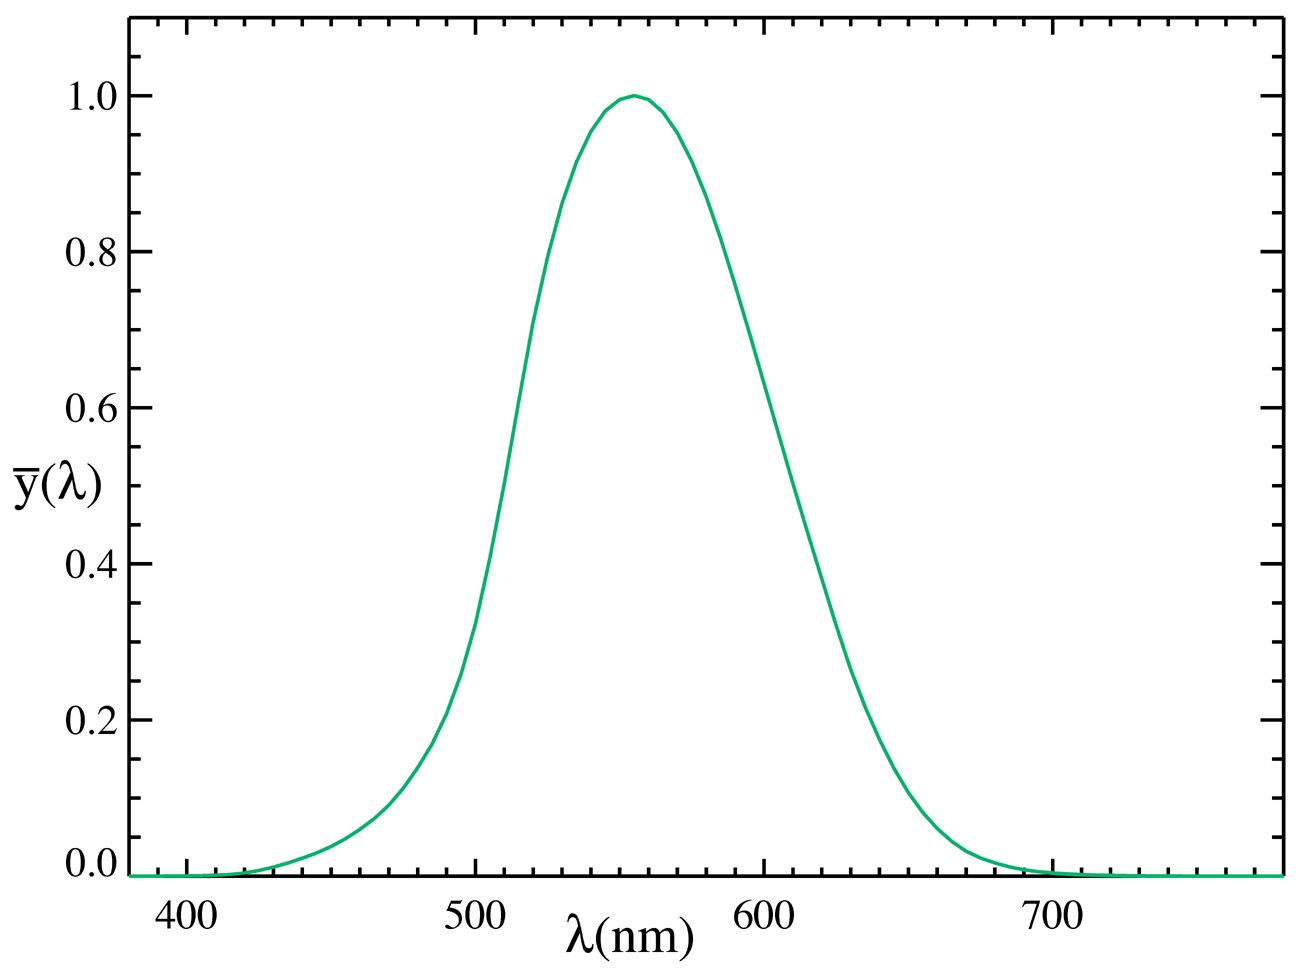
\includegraphics[width=7cm]{CIELuminosity}
  \end{center}
  \caption{Luminosity function $\bar{y}(\lambda)$: relation between the eye's sensitivity and the wavelength of light. The luminosity function is dimensionless, \cite{wiki}.}
  \label{fig:luminosityfunction}
  \end{figure}
\\ \indent The luminous flux corresponding to one Watt of radiation power at any wavelength is given by the product of $683$ $\textrm{lm/W}$ and the luminosity function at the same wavelength,
i.e. $683 \, \bar{y}(\lambda)$. Hence, the total luminous flux $\Phi$ has unit lumen (\textrm{lm}) and it is defined as:
\begin{equation}
\Phi = 683 \int_0^\infty \Phi_\textrm{r}(\lambda) \bar{y}(\lambda)\textrm{d}\lambda,
\end{equation}
where $\Phi_\textrm{r}(\lambda)$ is the spectral radiant flux, i.e. the radiant flux per unit wavelength (unit \textrm{W}/\textrm{m}). 
% Explain while integrals between 0 and infinity
The luminous emittance $M = M(x, \myangle)$ is the total flux emitted in all direction from a unit area. It is measured in lumens pr square meters (\textrm{lm}/$\textrm{m}^2$).
\\ \indent A beam of light can be described as a collection of parallel light rays, where a light ray can be interpreted as a path along which the energy travels. 
The luminous flux $\textrm{d}\Phi$ incident on a surface is called illuminance $E$ (unit $\textrm{lm}/\textrm{m}^2$)
and is defined as:
\begin{equation}
 E=E(x) = \frac{\textrm{d}\Phi}{\textrm{d}A}\;,
 \end{equation}
 where $\textrm{d}A$ is an infinitesimal area receiving radiation. The density of light emitted by a point source in a given direction is determined by the solid angle.\\ \indent
The solid angle in a given direction is expressed by a cone of rays emitted in that particular direction by a point source located at the center of the unit sphere, \cite{koshel2012illumination}. 
Let $\textrm{d}S$ be the area on the unit sphere subtended by the cone,
the infinitesimal solid angle $\textrm{d}\Omega$ is given by:
\begin{equation}\label{solid_angle}
\textrm{d}\Omega = \textrm{d}S= \sin(\theta)\textrm{d}\theta \textrm{d}\phi\,
\end{equation}
 where $\myangle$ and $\phi$ are the polar and the azimuthal angle that the normal $\boldsymbol{\nu}$ to $\textrm{d}A$ makes with the direction of the central line of $\textrm{d}\Omega$, respectively (see Figure \ref{fig:rad}).
The solid angle on the entire sphere is $\Omega = 4\pi$ and its unit is steradian $\textrm{sr}$, \cite{arecchi2007field}.
The luminous intensity $I$ (unit candela $\textrm{cd}=\textrm{lm}/\textrm{sr}$) is defined as the luminous flux $\textrm{d}\Phi$ per solid angle
$\textrm{d}\Omega$ and is given by:
\begin{equation}\label{intensity}
I = I(\myangle, \phi) = \frac{\textrm{d}\Phi}{\textrm{d}\Omega}\;.
\end{equation}
 \begin{figure}[h]
%\label{fig:cup}
  \begin{center}
  \includegraphics[width=6 cm]{SolidAngle}
  \end{center}
  \caption{Solid angle $\textrm{d}\Omega$ in a given direction $\myangle$ with $\myangle$ the angle that the central line forms with the normal to the area $\textrm{d}A$.}
  \label{fig:rad}
  \end{figure}
\\ \indent Let us now consider a finite source $\textrm{d}A$.
The luminance $L = L(\vect{x}, \myangle)$ (unit \textrm{cd} / \textrm{m}^2$) depends both on the position and the direction, it is the luminous flux per unit solid angle $\textrm{d}\Omega$ and  per unit projected area $\cos\myangle \textrm{d}A$.  $L$  is given by:
\begin{equation}\label{luminance1}
  L=L(\vect{x}, \myangle) = \frac{\textrm{d}\Phi}{\cos\myangle\textrm{d}A\textrm{d}\Omega}\,.
\end{equation}
\noindent Note that from ($\ref{intensity}$) and ($\ref{luminance1}$) we can derive a relation between the intensity and the luminance. 
The intensity $I$ emitted by the infinitesimal area $\textrm{d}A$ is given by:
\begin{equation}
I = \frac{\textrm{d}\Phi}{\textrm{d}\Omega}= L(\vect{x},\myangle)\cos\myangle\textrm{d}A \,.
\end{equation}
When the luminance is uniform over a finite area $A$, the luminous intensity emitted in the direction $\myangle$ is:
\begin{equation}
I(\vect{x}, \myangle) = I(\myangle) = L(\myangle) A \cos\myangle\,.
\end{equation}
Thus, when $L(\vect{x},\myangle)$ does not depend on the position and the direction (i.e. $L(\vect{x},\myangle)=L$), we obtain Lambert's cosine law:
\begin{equation}
I(\myangle) = I_0\cos\myangle\,.
\end{equation}
where $I_0 = I(\myangle = 0) = LA$. \\
\indent Finally, the \'{e}tendue $U$ (unit $[\textrm{m sr}]$) describes the ability of a source to emitt light or the capability of an optical system to receive light, \cite{zhu2011etendue}.
The quantity $ \textrm{d}U $ is defined as:
\begin{equation}\label{etendue}
\textrm{d}U = n^2 \cos\myangle\textrm{d}A\textrm{d}\Omega.
\end{equation}
where $n$ is the index of refraction of the medium in which the surface $A$ is immersed. In optics the \'{e}tendue is considered to be a volume in phase space  (or an area for two-dimensional systems). This concept will be clarified in Chapter \ref{chap:PS} in which we treat the phase space in more detail.
An important property of the \'{e}tendue is that it is conserved within an optical system in absence of absorption. We now show, using the approach of Chaves in \cite{chaves2015introduction}, 
how conservation of this quantity can be derived.
Consider a light ray emitted from an infinitesimal area $\textrm{d}A_1$ to the area $\textrm{d}A_2$. Suppose that the centers of $\textrm{d}A_1$ and $\textrm{d}A_2$ 
are located at a distance \variabile{d} to each other,  see Figure \ref{fig:etendue_conservation}.
\begin{figure}[h]
 \label{fig:etendue_conservation}
     \begin{center}
     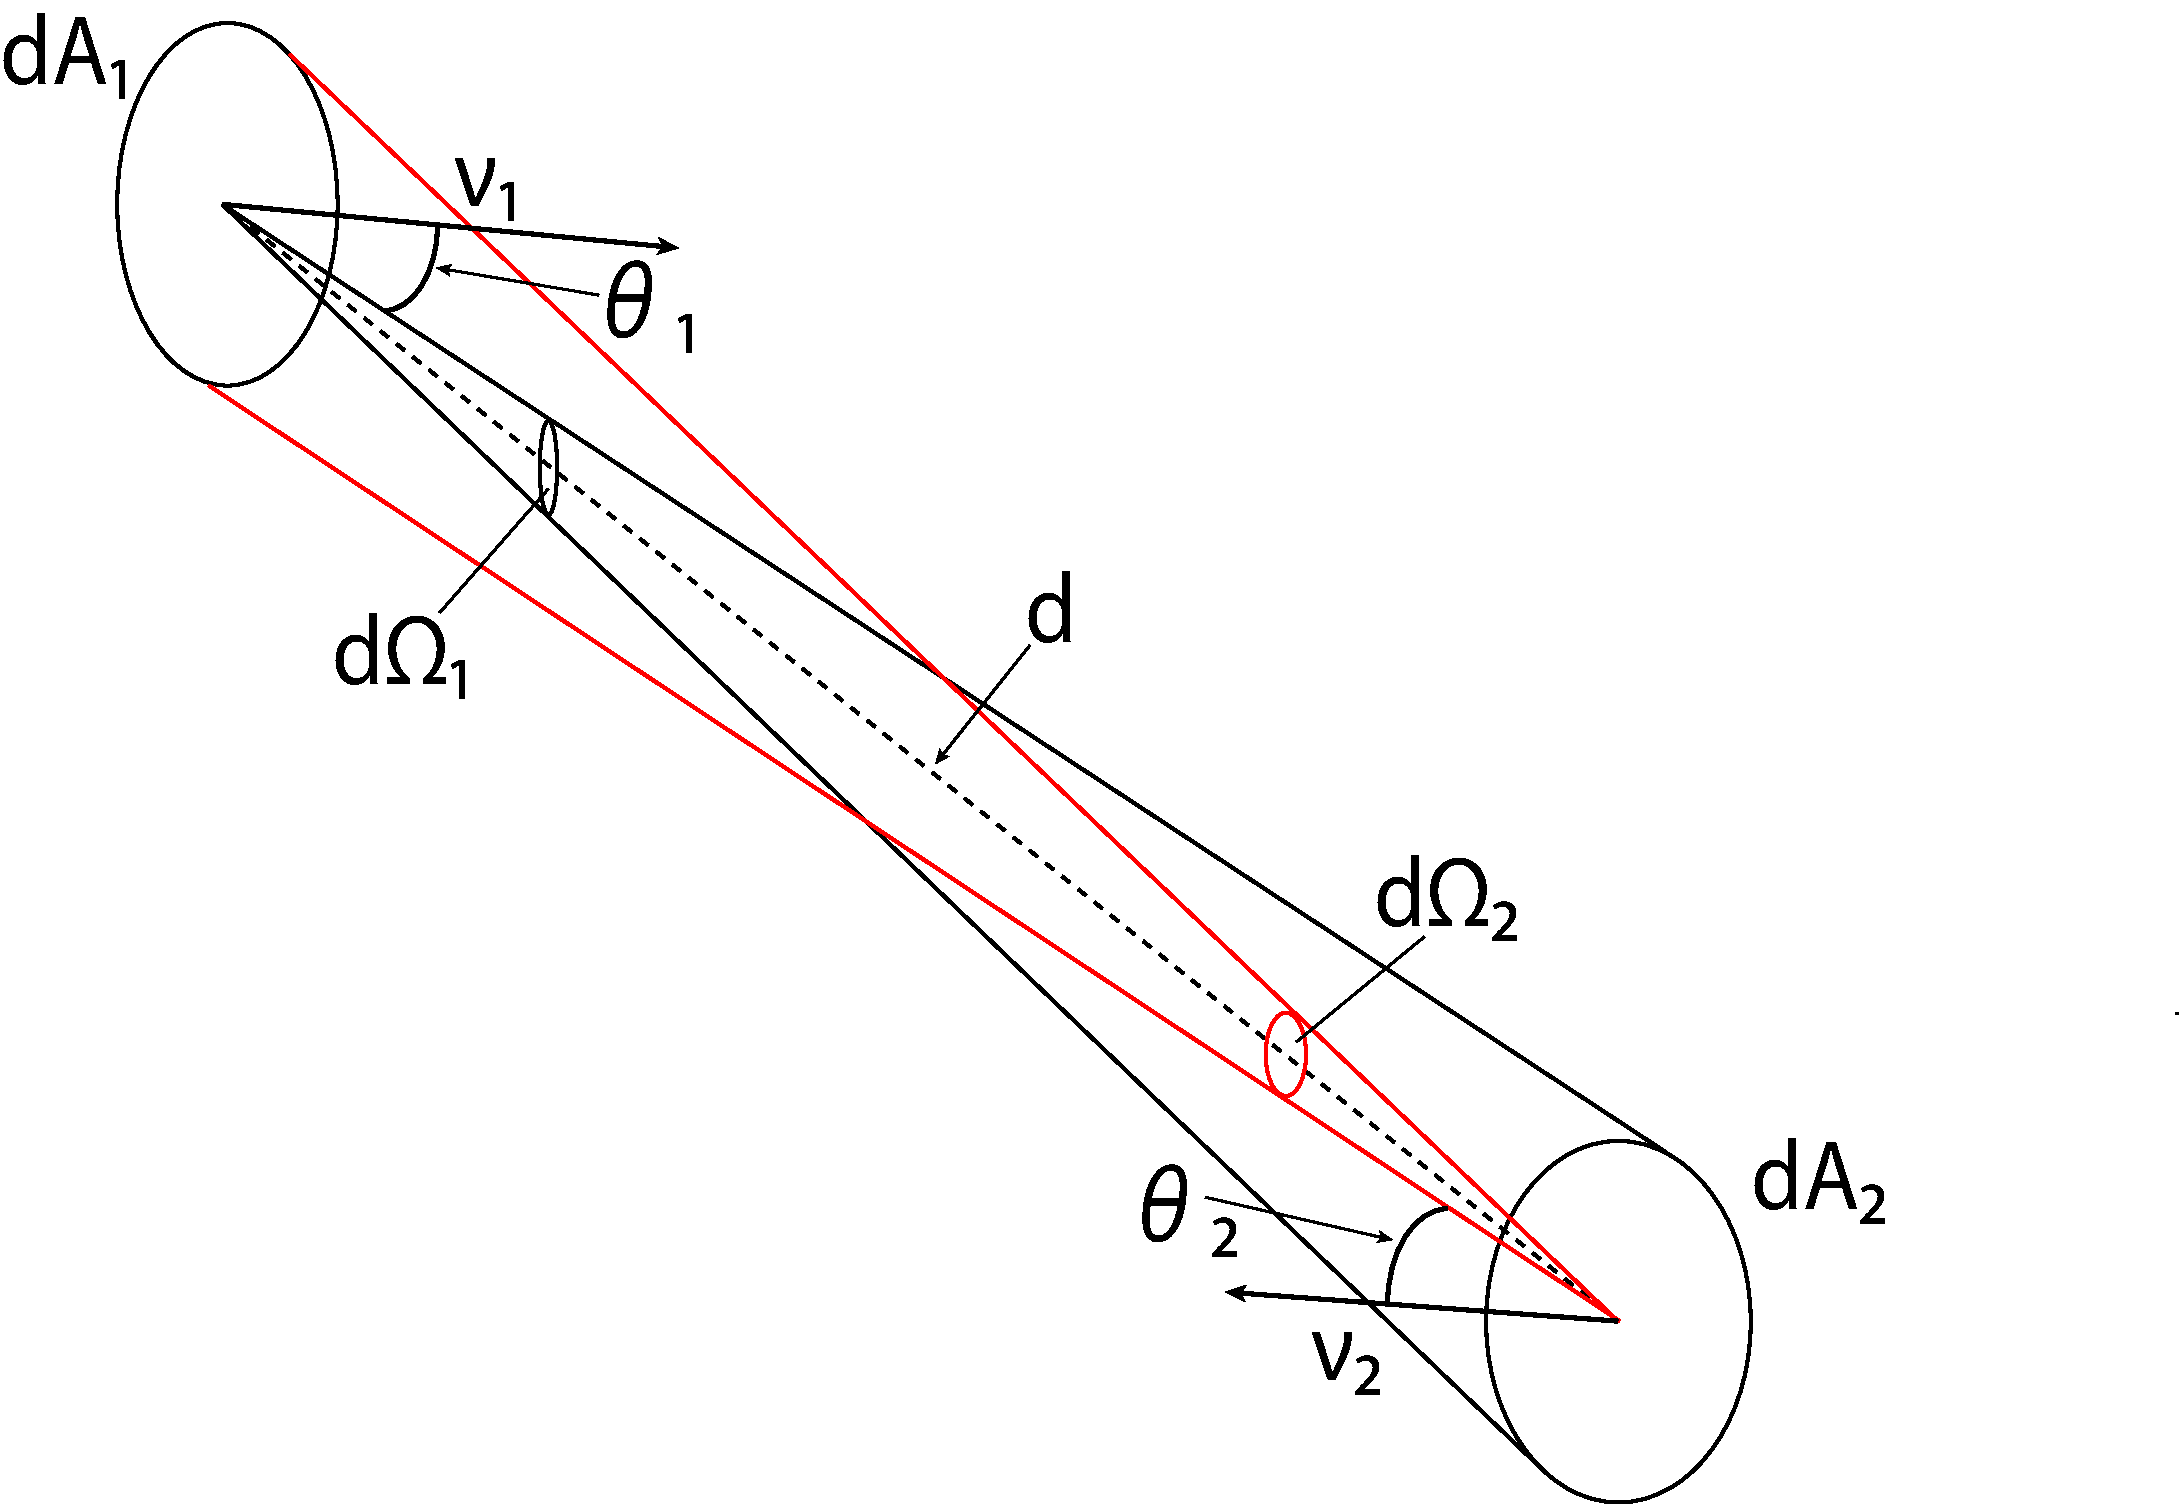
\includegraphics[width=10cm]{areas.pdf}
     \end{center}
     \caption{$\textrm{d}A_1$ and $\textrm{d}A_2$ are two surfaces with normals $\nu_1$ and $\nu_2$, respectively. Their centers are located at a distance \variabile{d}.
$\myangle_1$ and $\myangle_2$ are the angles made by the central ray with the normals $\nu_1$ and $\nu_2$, respectively.}
\label{fig:etendue_conservation}
 \end{figure}
Indicating with $\boldsymbol{\nu}_1$ and $\boldsymbol{\nu}_2$ the normals to the surfaces $\textrm{d}A_1$ and $\textrm{d}A_2$, respectively and with $\myangle_1$ and $\myangle_2$ the angles that the central ray forms with $\boldsymbol{\nu}_1$ and $\boldsymbol{\nu}_2$, respectively,
the flux $\textrm{d}\Phi_1$ passing through $\textrm{d}A_2$ coming from $\textrm{d}A_1$ and the corresponding solid angle $\textrm{d}\Omega_1 $ are defined as:
\begin{equation}
\begin{split}
\textrm{d}\Phi_1 &= L \cos\myangle_1 \textrm{d}A_1 \textrm{d}\Omega_1, \\
\textrm{d}\Omega_1 &= \frac{\textrm{d}A_2\cos(\myangle_2)}{\variabile{d}^2}\,.
\end{split}
\end{equation}
Similarly, the flux $\textrm{d}\Phi_2$ passing through $\textrm{d}A_1$ coming from $\textrm{d}A_2$ is equal to:
\begin{equation}\begin{split}
\textrm{d}\Phi_2 &= L \cos\myangle_2 \textrm{d}A_2 \textrm{d}\Omega_2\\
\textrm{d}\Omega_2 &= \frac{\textrm{d}A_1\cos\myangle_1}{\variabile{d}^2}\,.
\end{split}
\end{equation}
Then from Eq. (\ref{etendue}) we obtain the following relations: \begin{equation}
\begin{split}
\textrm{d}U_1 &= n^2 \textrm{d}A_1\cos\myangle_1\textrm{d}\Omega_1= \frac{n^2 \textrm{d}A_1\cos\myangle_1\textrm{d}A_2\cos\myangle_2}{\variabile{d}^2},\\
\textrm{d}U_2 &= n^2 \textrm{d}A_2\cos\myangle_2\textrm{d}\Omega_2= \frac{ n^2 \textrm{d}A_2\cos\myangle_2\textrm{d}A_1\cos\myangle_1	`}{\variabile{d}^2}
\end{split}
\end{equation}
for $\textrm{d}A_1$ and $\textrm{d}A_2$, respectively.
%From equation ($\ref{etendue1}$) and ($\ref{etendue2}$) 
From the previous equations we can conclude that $\textrm{d}U_1=\textrm{d}U_2$ and therefore the \'{e}tendue $\textrm{d}U$ is conserved along a beam of light. 
Since also the flux through the areas $\textrm{d}A_1$ and $\textrm{d}A_2$ is conserved, the following relation holds:
\begin{equation}\label{basicluminance}
L := n^2 \frac{\textrm{d}\Phi}{\textrm{d}U} = constant\,.
\end{equation}
 In the optical systems we will consider in this work, the source and the target are located in the same medium (air) with $n=1$, so the luminance $L$ equals the basic luminance $L^* = L/n^2$ at the source and the target of the system.\\
\indent In this thesis we consider two-dimensional optical systems. 
 Hence, the definitions of the photometric parameters have to be given in two dimensions. An infinitesimal line segment of length $\textrm{d}\variabile{a}$ that emits a light beam and the ray that makes an angle $\myangle$ with the normal $\boldsymbol{\nu}$ are considered, see Fig. \ref{fig:2Dsolidangle}. 

\begin{figure}[h]
 \label{fig:2Dsolidangle}
     \begin{center}
     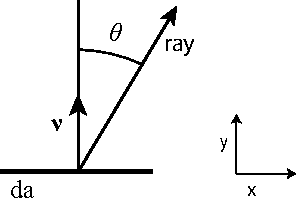
\includegraphics[width=7cm]{solidangle2D.pdf}
     \end{center}
     \caption{Ray emitted by an infinitesimal line segment $\textrm{d}a$ that makes an angle $\myangle$ with respect to the line normal $\boldsymbol{\nu}$.}
\label{fig:2Dsolidangle}
 \end{figure}

 The two-dimensional illuminance \big(unit $\big[\textrm{lm}/\textrm{m}\big]$\big) denotes the luminous flux falling on an infinitesimal line segment of length $\textrm{d}\variabile{a}$ 
and it is given by:
 \begin{equation}
 E=\frac{\textrm{d}\Phi}{\textrm{d}\variabile{a}}\;.
 \end{equation}
 The luminous intensity \big(unit $\big[\textrm{lm}/\textrm{rad}\big]$\big) is the luminous flux per angle $\textrm{d}\myangle$:
 \begin{equation}
 I=\frac{\textrm{d}\Phi}{\textrm{d}\myangle}\;.
 \end{equation}
 The two-dimensional luminance \big(unit $\big[\textrm{lm}/(\textrm{rad}\cdot \textrm{m})\big]$\big) is given by:
 \begin{equation}
 L= \frac{\textrm {d}\Phi}{\cos\myangle\,\textrm{d}\variabile{a} \,\textrm{d}\myangle}.
 \end{equation}
 Thus the following relation holds:
 \begin{equation}
 I = L(x, \myangle)\cos\myangle\,\textrm{d}\variabile{a}
 \end{equation}
where $x$ is a certain position at the light source $\textrm{d}a$.
 Finally, the \'{e}tendue $\textrm{d}U $ (unit $[\textrm{m}\cdot \textrm{rad}]$) in two dimensions is given by:
\begin{equation}\label{etendue2d}
\textrm{d}U = n\cos\myangle\textrm{d}\variabile{a}\,\textrm{d}\myangle.
\end{equation}
In order to determine the light distribution on a surface and to compute the photometric variables on that surface, we need to understand how the light emitted from the source propagates. In the field of geometric optics the light propagation is described by light rays.
The propagation of a light ray traveling through  different media is determined by the reflection and refraction law.
In the following we introduce these two laws and we explain the total internal reflection phenomenon.
\section{Reflection and refraction law}\label{sec:reflection}
A light ray is described by a position vector \vect{x} on a surface and a direction vector \vect{t} and can be parameterized by the arc length \variabile{s}.
Light rays travel in a homogeneous medium along straight lines, once they hit a reflective surface their direction changes.
 Denoting with $\vect{t}_\textrm{i}$ the direction of the incident ray and with $\boldsymbol{\nu}$ the unit normal to the surface at the location of incidence, the direction $\vect{t}_\textrm{r}$ of the reflected ray is given by:
 \begin{equation}\label{Reflection}
  \vect{t}_\textrm{r} = \vect{t}_\textrm{i}-2 (\vect{t}_\textrm{i}\boldsymbol{\cdot}\boldsymbol{\nu})\boldsymbol{\nu}\,,
\end{equation}
where the vectors $\vect{t}_\textrm{i}$ and $\boldsymbol{\nu}$ are unit vectors and $\vect{t}_\textrm{i}\boldsymbol{\cdot}\boldsymbol{\nu}$ indicates the scalar product between 
$\vect{t}_\textrm{i}$ and $\boldsymbol{\nu}$. 
From Eq. (\ref{Reflection}) it follows that the vector  $\vect{t}_\textrm{r}$ is a unit vector too, indeed considering the scalar product $(\vect{t}_\textrm{r},\vect{t}_\textrm{r})$ we conclude:
\begin{equation}\label{unit_vector}
\vect{t}_\textrm{r}\boldsymbol{\cdot}\vect{t}_\textrm{r} = \vect{t}_\textrm{i}\boldsymbol{\cdot}\vect{t}_\textrm{i} 
- 4(\vect{t}_\textrm{i}\boldsymbol{\cdot}\boldsymbol{\nu})(\vect{t}_\textrm{i}\boldsymbol{\cdot}\boldsymbol{\nu})+
4(\vect{t}_\textrm{i}\boldsymbol{\cdot}\boldsymbol{\nu})^2(\boldsymbol{\nu}\boldsymbol{\cdot}\boldsymbol{\nu})=1 .
\end{equation} 
The vectors $\vect{t}_\textrm{i}$, $\vect{t}_\textrm{r}$ and $\boldsymbol{\nu}$ live all in the same plane.
Defining the incident angle $\myangle_\textrm{i}$ and the reflective angle $\myangle_\textrm{r}$ such that $\myangle_\textrm{i}$, $\myangle_\textrm{r} \in[0, \pi/2)$.
%\begin{equation}
%\cos{\myangle_\textrm{i}} = -\vect{t}_\textrm{i}\cdot \boldsymbol{\nu} \qquad \mbox{and} \qquad \cos{\myangle_\textrm{r}} = \vect{t}_\textrm{r} \cdot\boldsymbol{\nu}\,,
%\end{equation}
the reflection law states that $\myangle_\textrm{i}=\myangle_\textrm{r}$, see Fig. \ref{fig:Snell}.
\begin{figure}[h]
 \label{fig:Snell}
     \begin{center}
     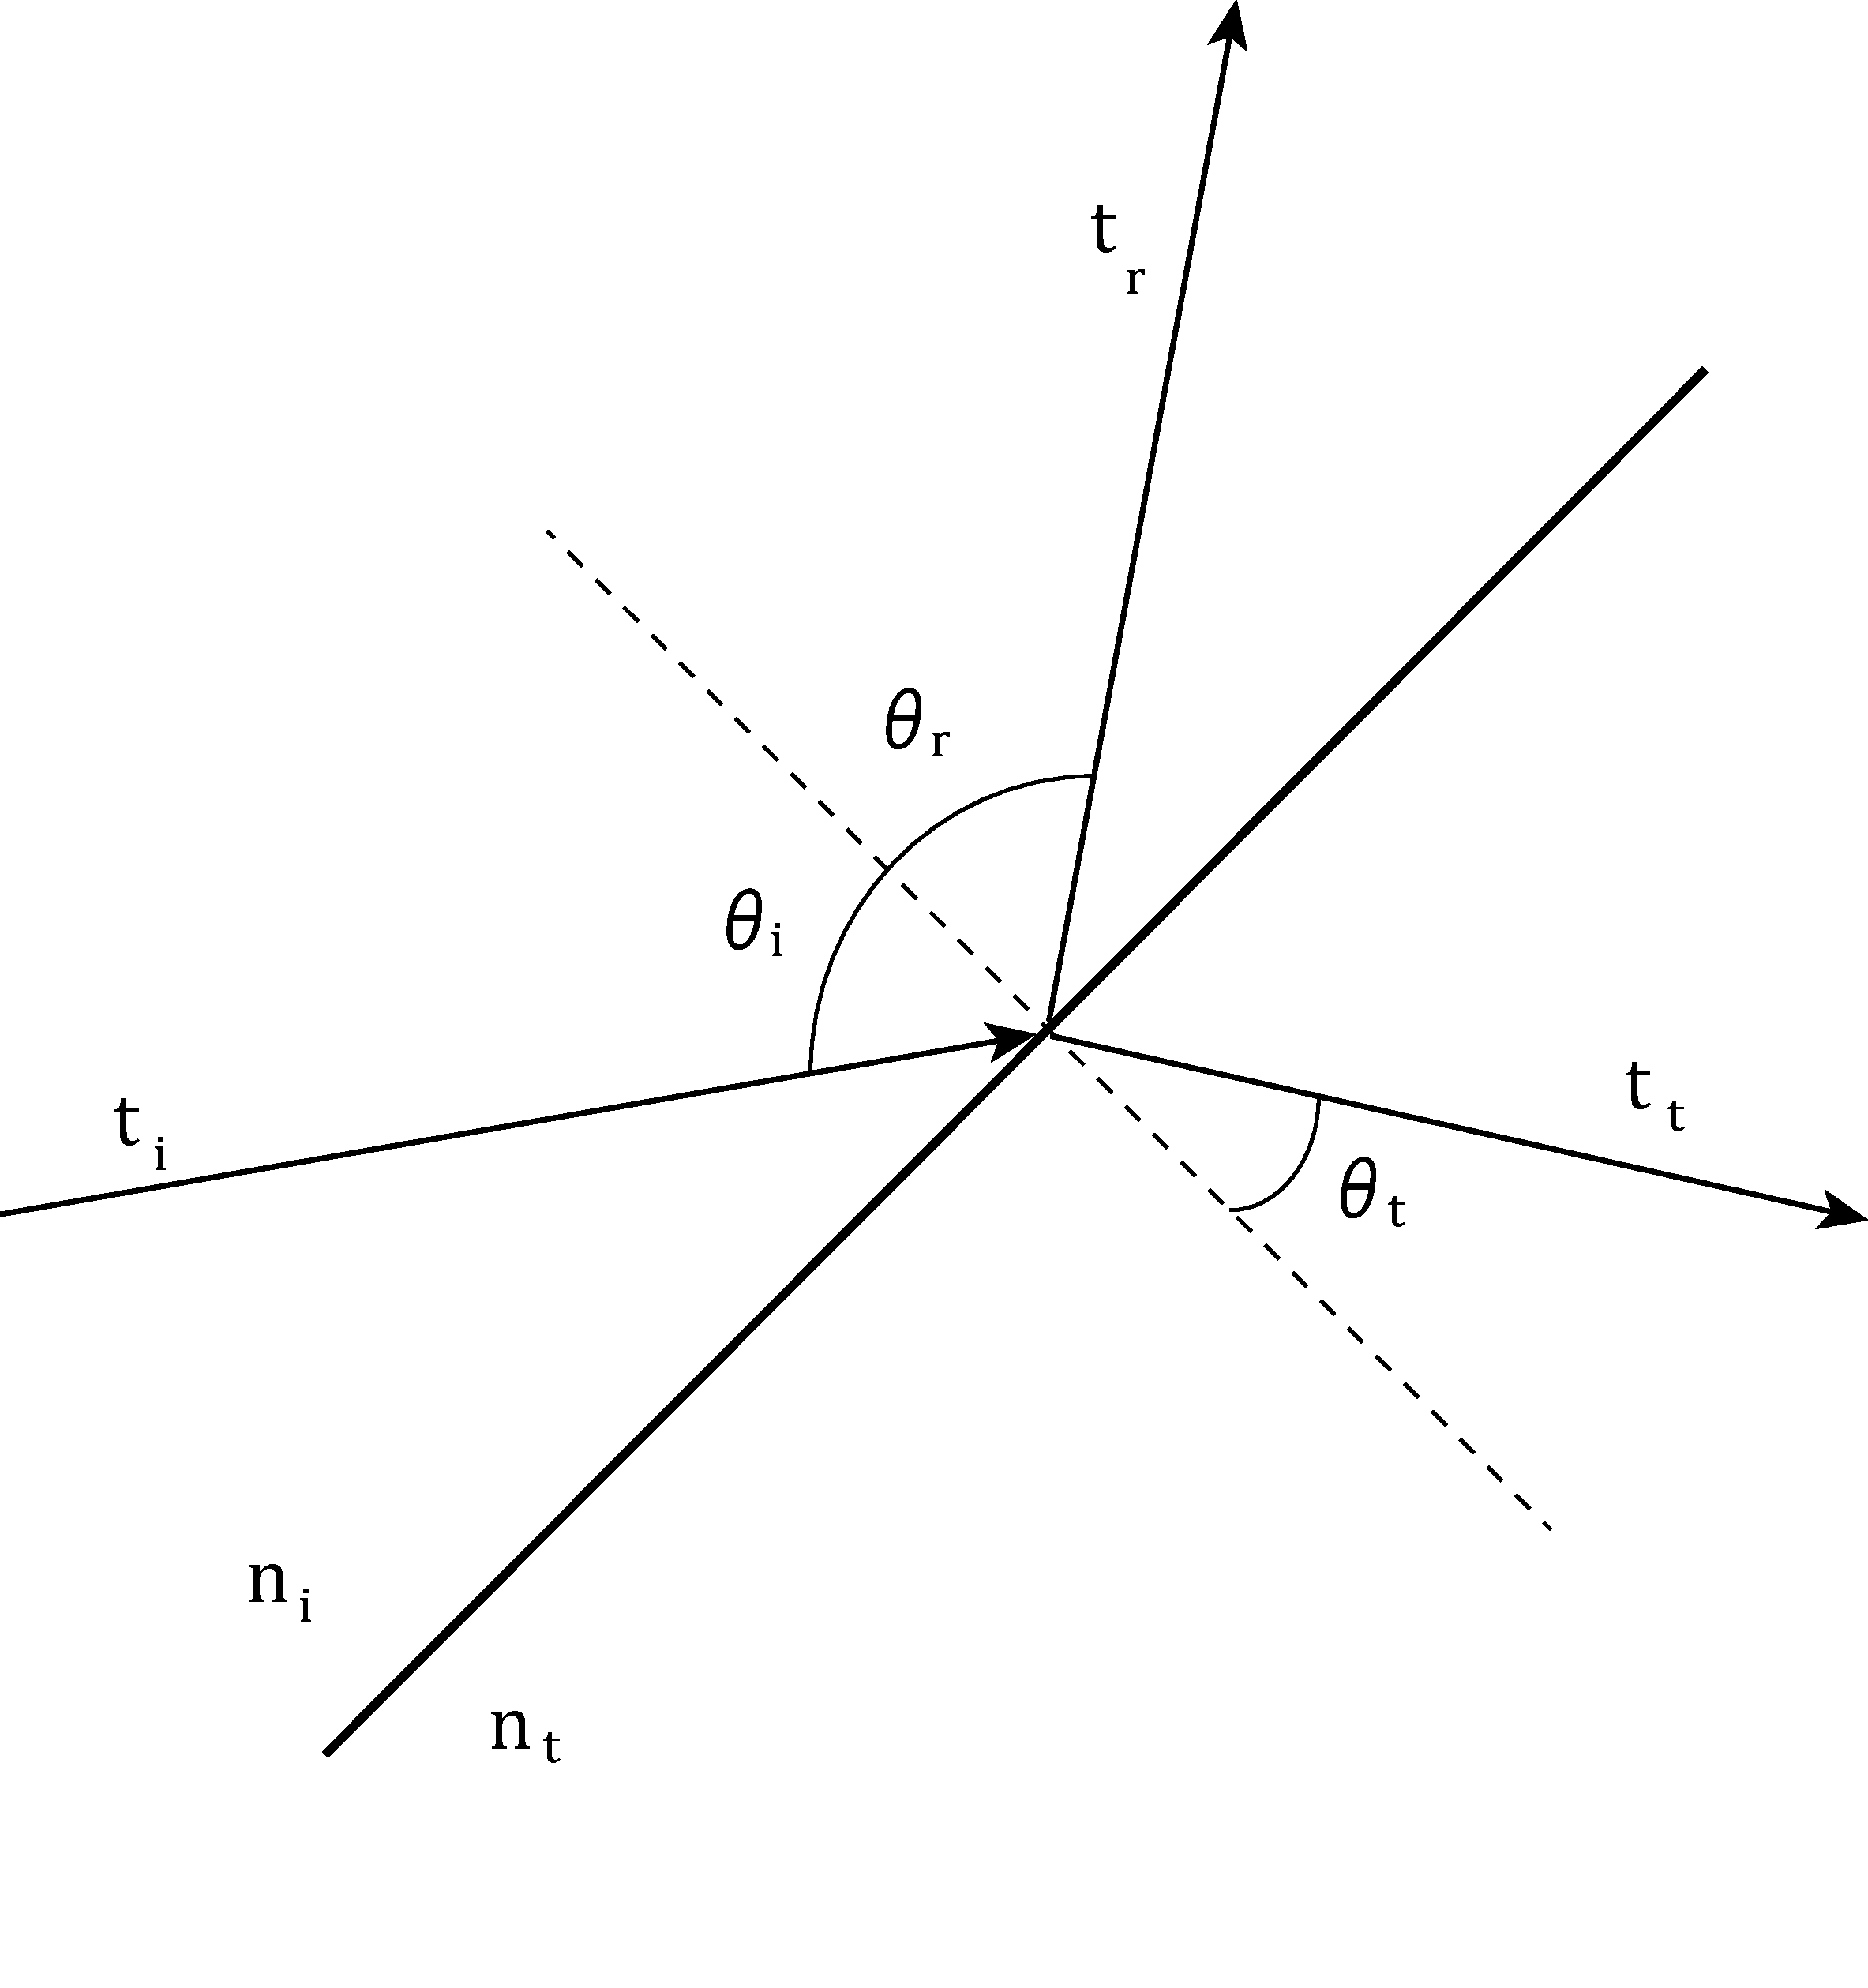
\includegraphics[width=8cm]{reflection}
     \end{center}
     \caption{Propagation of a ray through two different media with index of refraction $n_\textrm{i}$ and $n_\textrm{t}$.}% \bolsymbol{$\nu$} is the normal to the surface $A$ that the incident ray hits.
%$\vect{t}_i$, $\vect{t}_r$ and $\vect{t}_t$ are the direction vectors of the incident, reflected and refracted (or transmitted) ray, respectively. }}
%\myangle$_{i}$, \myangle$_{r}$ and \myangle$_{t}$ are the angles between \bolsymbol{$\nu$} and the incident, reflected and transmitted ray, respectively.}}
\label{fig:Snell}
 \end{figure}
\\ When a ray propagates through two different media, its direction changes according to the law of refraction. 
Indicating with $n_\textrm{i}$ the index of refraction of the medium in which the incident ray travels and with 
$n_\textrm{t}$ the index of refraction of the medium of the transmitted ray, the direction $\vect{t}_\textrm{t}$ of the transmitted ray is given by:
\begin{equation}\label{Refraction}
\vect{t}_\textrm{t} = n_{\textrm{i},\textrm{t}}\,\vect{t}_\textrm{i}+
\Big[\sqrt{1-n_{\textrm{i},\textrm{t}}^2+
n_{\textrm{i},\textrm{t}}^2(\boldsymbol{\nu}\boldsymbol{\cdot}\vect{t}_\textrm{i})^2}
-n_{\textrm{i},\textrm{t}}(\boldsymbol{\nu}\boldsymbol{\cdot}\vect{t}_\textrm{i}) \Big]\boldsymbol{\nu}\,,
\end{equation}
where $n_{\textrm{i},\textrm{t}}=n_\textrm{i}/n_\textrm{t}$, \cite{chaves2015introduction}.
 Note that in Eq. (\ref{Reflection}) the direction of the normal $\boldsymbol{\nu}$ to the surface is not relevant for the computation of the direction of the reflective ray, since:
\begin{equation}
\vect{t}_\textrm{r} = \vect{t}_\textrm{i}-2(\vect{t}_\textrm{i}\boldsymbol{\cdot}\boldsymbol{\nu})\boldsymbol{\nu}= \vect{t}_\textrm{i}-2(\vect{t}_\textrm{i}\boldsymbol{\cdot}-\boldsymbol{\nu})(-\boldsymbol{\nu}) ,
\end{equation}
however, this is not the case for Eq. (\ref{Refraction}), therefore in the latter case we need to specify the direction of $\boldsymbol{\nu}$ which is usually chosen in such a way that the angle that it forms with the incident ray $\vect{t}_\textrm{i}$ is smaller than or equal to $\pi/2$. Hence, if $(\vect{t}_\textrm{i}, \boldsymbol{\nu})\leq0$ the normal $\boldsymbol{\nu}$ directed inside the same medium in which travels the incident ray is taken as in Fig. \ref{fig:Snell}, 
otherwise the normal $-\boldsymbol{\nu}$ directed inside the same medium in which the transmitted ray will travel has to be considered.
\\\indent
Eq. (\ref{Refraction}) is only valid for 
\begin{equation}\label{tir}
1-n_{\textrm{i},\textrm{t}}^2+n_{\textrm{i},\textrm{t}}^2(\boldsymbol{\nu}\boldsymbol{\cdot}\vect{t}_\textrm{i})^2\geq 0 
\end{equation} which implies that
\begin{equation}
\frac{n_\textrm{t}}{n_\textrm{i}}\geq \sqrt{1-(\boldsymbol{\nu}\boldsymbol{\cdot}\vect{t}_\textrm{i})^2}
\end{equation}
from which we obtain:
\begin{equation}
 %n_\textrm{t}\geq n_\textrm{i}\sqrt{1-\cos^2\myangle_\textrm{i}}= 
 n_\textrm{t}\geq n_\textrm{i} \sin\myangle_\textrm{i}\,.
\end{equation}
 The angle $\myangle_{\textrm{c}}$ for which the equality holds is
\begin{equation}\label{critical}
\myangle_{\textrm{c}} = \arcsin\Big(\frac{n_\textrm{t}}{n_\textrm{i}}\Big)
\end{equation} and it is called the critical angle, \cite{chaves2015introduction}.
%Note that the condition $\frac{n_t}{n_i}<1$ is verified as in this case $\sin(\myangle_\textrm{i})<1$.
When the incident angle $\myangle_{\textrm{i}}$ is exactly equal to the critical angle $\myangle_{\textrm{c}}$, the square root in Eq. (\ref{Refraction}) is zero and the inner product $(\vect{t}_\textrm{t},\boldsymbol{\nu})=0$, hence the transmitted ray propagates parallel to the refractive surface. 
When $\myangle_{\textrm{i}}>\myangle_{\textrm{c}}$ the light ray is no longer refracted but is only reflected by the surface. This phenomenon is called total internal reflection (TIR). When TIR occurs, $100\%$ of light is reflected and there is no loss of energy. Therefore, optical systems designed such that rays are reflected by TIR are very efficient. Lght that hits an ordinary refractive surface can be reflected and refracted. The energy that is reflected and refracted is determined by the Fresnel's coefficients.
In the next paragraph an overview of the Fresnel coefficients is given.

\section{Fresnel's equations}\label{sec:fresnel}
In order to derive Fresnel's equations we need to describe light as an electromagnetic wave. 
It is therefore useful to study the light propagation from the perspective of electromagnetic theory which gives information about the incident, reflected and transmitted radiant flux density that are denoted with $E_i$, $E_r$ and $E_t$, respectively.  
Any component of the electric field $\boldsymbol{\mathcal{E}}$ can be written as
\begin{equation}\label{electric_field}
\boldsymbol{\mathcal{E}}(\vect{x}, \mytime) = \boldsymbol{\mathcal{E}}_0(\vect{x} )e^{i( \vect{k}\boldsymbol{\cdot}\vect{x}-\omega \mytime )}
\end{equation}
where \vect{x} is the position vector and $T$ is the time. The amplitude $\boldsymbol{\mathcal{E}}_0(\vect{x})$ is constant in time and $\omega = \frac{c k}{n}$ is the value of the angular frequency with $c$ the velocity of light and $n$ the index of refraction in which the wave is traveling, which is the ratio of the speed of light $c$ in vacuum and the speed of light $v$ in the material. Note that the angular frequency can be also written as $\omega = vk$, in particular when a wave travels in vacuum $n=1$ and $\omega=ck$. The vector \vect{k} has the same direction of the wave and its absolute value 
$|\vect{k}| = k = \frac{2\pi}{\lambda}$ is the wave number in vacuum, with $\lambda$ the wavelength. Similarly, the magnetic field has the form:
\begin{equation}
\boldsymbol{\mathcal{B}}(\vect{x}, \mytime) = \boldsymbol{\mathcal{B}}_0(\vect{x}) e^{i( \vect{k}\boldsymbol{\cdot} \vect{x}-\omega \mytime )}\,.
\end{equation}
Light can be seen as an electromagnetic wave, that is an oscillating electric field $\boldsymbol{\mathcal{E}}$ and an oscillating magnetic filed $\boldsymbol{\mathcal{B}}$ which propagates  always perpendicular to $\boldsymbol{\mathcal{E}}$. Th eelectric field oscillates perpendicular to the wave propagation.
Light is said to be polarized if the direction of the electic field is well defined. When the electric field propagates in different directions we talk about unpolarized light. 
By convention, we refer to the light's polarization as the direction of the electric field $\boldsymbol{\mathcal{E}}$, \cite{feynman1964feynman} with respect to the incident plane that is defined by the incident and reflected rays as is shown in Fig. \ref{fig:planeofincidence}. 
\begin{figure}[h]
 \label{fig:planeofincidence}
     \begin{center}
     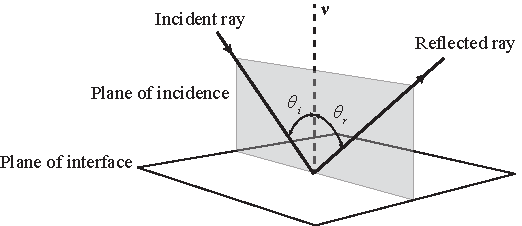
\includegraphics[width=10cm]{plane_of_incidence1}
     \end{center}
     \caption{Light ray that hits a mirror located on the reflecting plane. The incident and the reflected ray leave in the same plane of the normal to the mirror that is called plane of incident.}
\label{fig:planeofincidence}
 \end{figure}
\\ \indent In order to derive the Fresnel's coefficients the polarization of light must to be taken into account.
Those coefficients are obtained considering Maxwell's equations and the boundary conditions due to the conservation of energy.
The details of Fresnel's equations are widely explained in the literature. 
In the following we provide Fresnel coefficients and we briefly explain their physical interpretation. We refer the reader to \cite{born2013principles, hecht1998hecht} for more details. 
Fresnel's coefficients can also be derived using a different approach that does not involve Maxwell's equations, this method is explained in \cite{feynman2011feynman}.  
The following particular cases of light's polarization need are considered. 
\begin{enumerate}
\item $\boldsymbol{\mathcal{E}}$ is perpendicular to the plane of incidence (see Fig. \ref{fig:electric_field}). In this case light is said to be $s$-polarized.
\item $\boldsymbol{\mathcal{E}}$ is parallel to the plane of incidence (see Fig. \ref{fig:electric_field_p}). In this case light is said to be $p$-polarized.
\end{enumerate}
\begin{figure}[h]
 \label{fig:electric_field}
     \begin{center}
     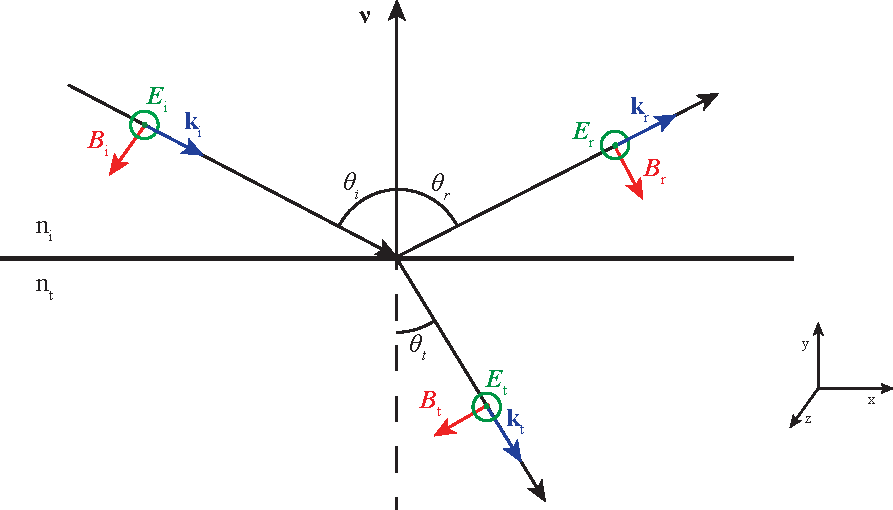
\includegraphics[width=8cm]{electric_field}
     \end{center}
     \caption{Propagation of an electromagnetic wave where $\boldsymbol{\mathcal{E}}$ is perpendicular to the incident plane. The components of $\boldsymbol{\mathcal{E}}$ are is indicated with the green circles.
%, they live in the $(\variabile{x},\variabile{z})$ plane and they are oriented in the positive direction of $\variabile{z}$. 
The components of $\boldsymbol{\mathcal{B}}$ are indicated with red arrows.}
% and they are located in the $(\variabile{x}, \variabile{z})$ plane.}
\label{fig:electric_field}
 \end{figure}
\begin{figure}[h]
 \label{fig:electric_field_p}
     \begin{center}
     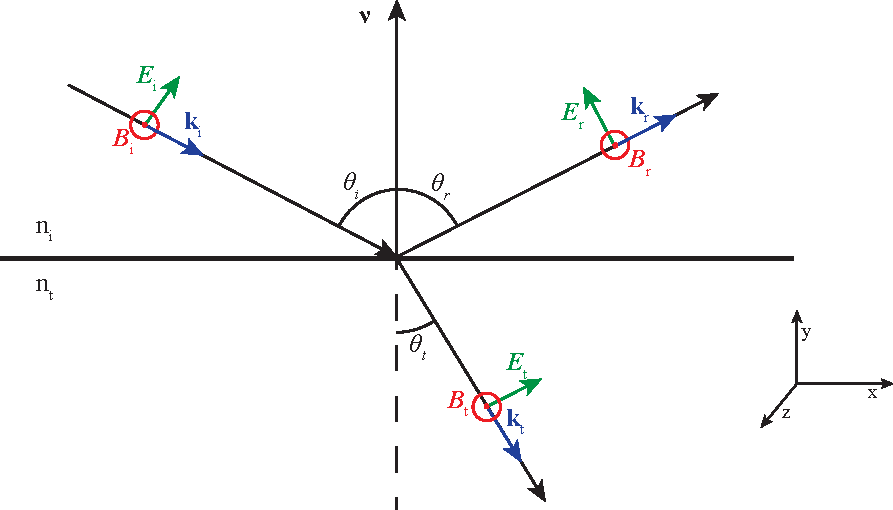
\includegraphics[width=8cm]{electric_field_p}
     \end{center}
 \caption{Propagation of an electromagnetic wave where $\boldsymbol{\mathcal{E}}$ is parallel to the incident plane. The components of $\boldsymbol{\mathcal{B}}$ are indicated with the red circle.
%, they are in the $(\variabile{x},\variabile{z})$ plane and they are oriented in the positive direction of $\variabile{z}$. 
The components of $\boldsymbol{\mathcal{E}}$ are indicated with greed arrows.}
%and they are located in the $(\variabile{x}, \variabile{z})$ plane.}
\label{fig:electric_field_p}
 \end{figure}
Energy conservation gives the boundary conditions of the electromagnetic field at the plane of the interface (which is perpendicular to the incident plane). In the following we derive Fresnel's coefficients for case $1$. Similarly, the Fresnel's coefficients can be derived for the second case.\\ 
\indent For $s$-polarized light the tangential components of $\boldsymbol{\mathcal{E}}$ and $\boldsymbol{\mathcal{B}}/\mu$ across the boundary between the two different media must be continuous. The continuity of the tangential component of $\boldsymbol{\mathcal{E}}$ leads to:
\begin{equation}\label{Econservation}
|\boldsymbol{\mathcal{E}}_{0\textrm{i}}|+|\boldsymbol{\mathcal{E}}_{0\textrm{r}}|= |\boldsymbol{\mathcal{E}}_{0\textrm{t}}|,
\end{equation} 
%where we have indicated with $\mathcal{E}_{0\textrm{i}}$, $\mathcal{E}_{0\textrm{r}}$ and $\mathcal{E}_{0\textrm{t}}$
%the magnitudes of $\boldsymbol{\mathcal{E}}_{0\textrm{i}}$, $\boldsymbol{\mathcal{E}}_{0\textrm{r}}$ and $\boldsymbol{\mathcal{E}}_{0\textrm{t}}$, respectively.
while the continuity of the tangential component of $\boldsymbol{\mathcal{B}}/\mu$ gives:
\begin{equation}\label{Bconservation}
-\frac{|\boldsymbol{\mathcal{B}}_{0,\textrm{i}}|}{\mu_\textrm{i}}\cos\myangle_{\textrm{i}}+\frac{|\boldsymbol{\mathcal{B}}_{0,\textrm{r}}|}{\mu_\textrm{r}}\cos\myangle_{\textrm{r}} = 
-\frac{|\boldsymbol{\mathcal{B}}_{0,\textrm{t}}|}{\mu_\textrm{t}}\cos\myangle_{\textrm{t}},
\end{equation}
where the negative sign in front of $|\boldsymbol{\mathcal{B}}_{0,\textrm{i}}|$ and $|\boldsymbol{\mathcal{B}}_{0,\textrm{t}}|$ is due to the convention that a positive direction is considered with increasing $\variabile{x}$.
%where we have indicated with $\mathcal{B}_{\textrm{i}}$, $\mathcal{B}_{\textrm{r}}$ and $\mathcal{B}_{\textrm{t}}$
%the absolute values of $\boldsymbol{\mathcal{B}}_{\textrm{i}}$,$\boldsymbol{\mathcal{B}}_{\textrm{r}}$ and $\boldsymbol{\mathcal{B}}_{\textrm{t}}$, respectively.
Since $\boldsymbol{\mathcal{B}} = \boldsymbol{\mathcal{E}}/v$, Eq. (\ref{Bconservation}) can be written as 
\begin{equation}
\frac{1}{\mu_{\textrm{i}}v_{\textrm{i}}}(|\boldsymbol{\mathcal{E}}_{0,\textrm{i}}|-|\boldsymbol{\mathcal{E}}_{0,\textrm{r}}|)\cos\myangle_{\textrm{i}} = \frac{1}{\mu_{\textrm{t}}v_{\textrm{t}}}|\boldsymbol{\mathcal{E}}_{0,\textrm{t}}|\cos\myangle_{\textrm{t}},
\end{equation}
where we employed the fact that $v_{\textrm{i}}= v_{\textrm{r}}$, and $\myangle_{\textrm{i}}= \myangle_{\textrm{r}}$. 
Using Eq. (\ref{electric_field}) and $n = c/v$, the previous equation becomes:
\begin{equation}
\frac{n_{\textrm{i}}}{\mu_{\textrm{i}}}(|\boldsymbol{\mathcal{E}}_{0\textrm{i}}|-|\boldsymbol{\mathcal{E}}_{0\textrm{r}}|)\cos\myangle_{\textrm{i}} = \frac{n_{\textrm{t}}}{\mu_{\textrm{i}}}|\boldsymbol{\mathcal{E}}_{0\textrm{t}}|\cos\myangle_{\textrm{t}}
\end{equation}
Finally,  assuming that $\mu_{\textrm{i}}=\mu_{\textrm{t}}=\mu_{0}$ and employing Eq. (\ref{Econservation}) we obtain:
\begin{equation} \label{Fresnel_perpendicular}
\begin{split}
r_{s} & =\frac{|\boldsymbol{\mathcal{E}}_{0 \textrm{r}}|_{s}}{|\boldsymbol{\mathcal{E}}_{0\textrm{i}}|_s} = 
\frac{n_\textrm{i}\cos\myangle_\textrm{i}-n_\textrm{t} \cos\myangle_\textrm{t}}{n_\textrm{i}
\cos\myangle_\textrm{i}+n_\textrm{t}\cos\myangle_\textrm{t}},\\
t_{s} & = \frac{|\boldsymbol{\mathcal{E}}_{0 \textrm{t}}|_s}{|\boldsymbol{\mathcal{E}}_{0\textrm{i}}|_s} 
=\frac{2n_\textrm{i}\cos\myangle_\textrm{i}}{n_\textrm{i}\cos\myangle_\textrm{i}+n_\textrm{t}\cos\myangle_\textrm{t}}.\\
\end{split}
\end{equation}
The coefficients $r_s$ and $t_s$ are amplitude coefficients for the reflected and transmitted light.
They are the perpendicular components of $r$ and $t$ for $s$-polarized light.
Using Snell's law, that is $n_{\textrm{i}}\sin\myangle_{\textrm{i}} = n_{\textrm{t}}\sin\myangle_{\textrm{t}}$, the relations for $r_s$ and $t_s$ are simplified as follows:
\begin{equation} \label{simple_Fresnel}
\begin{split}
r_{s} & = -\frac{\sin(\myangle_i-\myangle_t)}{\sin(\myangle_i+\myangle_t)},\\
t_{s} & = -\frac{2\sin \myangle_t \cos \myangle_i}{\sin(\myangle_i+\myangle_t)}\,.
\end{split}
\end{equation}
\indent A similar argument for the $p$-polarized light leads to the calculation of the parallel components $r_p$ and $t_p$ of $r$ and $t$. 
In case $\boldsymbol{\mathcal{E}}$ is parallel to the plane of incidence the amplitude coefficients are:
\begin{equation}\label{Fresnel_parallel}
\begin{split}
r_{p} & = \frac{n_t\cos\myangle_i-n_i \cos\myangle_t}{n_i \cos\myangle_t+n_t\cos\myangle_i},\\
t_{p} & =  \frac{2n_i\cos\myangle_i}{n_i\cos\myangle_t+n_t\cos\myangle_i}\,,
\end{split}
\end{equation}
and their simplified relations are:
\begin{equation} \label{simple_Fresnel}
\begin{split}
r_{p} & =  \frac{\tan(\myangle_i-\myangle_t)}{\myangle_i+\myangle_t},\\
t_{p} & = \frac{2\sin \myangle_t \cos \myangle_i}{\sin(\myangle_i+\myangle_t)\cos(\myangle_i- \myangle_t)}.
\end{split}
\end{equation}
Furthermore, it can be checked that
 \begin{equation}
\begin{split}
t_s-r_s &= 1, \\
t_p+r_p &=  1.
\end{split}
\end{equation}
The amplitude coefficients are shown in Fig. \ref{fig:coefficients} for the case in which light travels from a less dense to a more dense medium ($n_i<n_t$), that is external reflection. 
In Fig. \ref{fig:coefficients2} the reflection coefficients are shown for the case in which $n_i>n_t$, that is internal reflection. Note from Fig. \ref{fig:coefficients} that $r_p$ approaches to $0$ when $\myangle_i$ approaches to $\myangle_p$ and it gradually decreases reaching $-1$ for an incident angle $\myangle_i=90^\circ$. The angle $\myangle_p$ is called Brewster's angle or polarization angle as only the component perpendicular to the incident plane is reflected at that angle and therefore light is perfectly polarized. Similarly, Fig. \ref{fig:coefficients2} shows that $r_p=0$ for $\myangle_i= \myangle_{p\prime}$. It can be show that $\myangle_p+ \myangle_{p\prime}= 90^\circ$. Both $r_p$ and $r_s$ reach $1$ when $\myangle_i= $ $\myangle_c$. $\myangle_c$ is called the critical angle. Light that hits the incident plane with an incident angle equal to or greater than the critical angle is totally reflected back and no transmitted light is observed. This phenomenon is called total internal reflection. 
\begin{figure}[h]
  \begin{minipage}[h]{0.4\textwidth}
    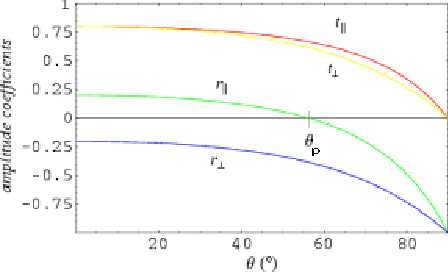
\includegraphics[width=\textwidth]{amplitude_coefficients2.pdf}
    \caption{Amplitude coefficients of reflection and transmission as a function of the incident angle $\myangle_i$  in the case of external reflection, i.e. $n_t<n_i$
($n_t = 1$ and $n_i=1.5$). $\myangle_p$ is the polarization angle, \cite{hecht1998hecht}.}
    \label{fig:coefficients}
  \end{minipage} \hspace{2.5cm}
  \begin{minipage}[h]{0.4\textwidth}
    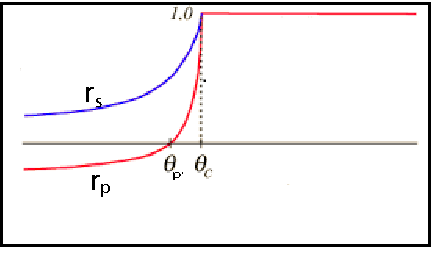
\includegraphics[width=\textwidth]{rprs.pdf}
    \caption{Reflection coefficients as a function of the incident angle $\myangle_i$ in the case of internal reflection, i.e. $n_t>n_i$
($n_t = 1.5$ and $n_i=1$). $\myangle_{p\prime}$ is the polarization angle and $\myangle_c$ is the critical angle, \cite{hecht1998hecht}.}
   \label{fig:coefficients2}
 \end{minipage}
\end{figure}\\
\indent The  we introduce the Poynting vector \vect{P} that defines the energy flux of an electromagnetic field. 
It is measured in $[\textrm{W}/\textrm{m}^2]$, and it is given by:
\begin{equation}
\vect{P} = \frac{1}{\mu}\Big(\boldsymbol{\mathcal{E}}\boldsymbol{\times} \boldsymbol{\mathcal{B}}\Big),
\end{equation}
where $\mu = \frac{1}{\varepsilon v^2}$ is the permeability and $\varepsilon$ the permittivity of the medium.
 In the following, the parameters for vacuum are indicated with the subscript $0$. All quantities defined in the media of the incident, reflective and transmitted light are indicated with the subscripts \textrm{i}, \textrm{r} and \textrm{t}, respectively. Optical rays are perpendicular to the wave front of an electromagnetic wave and parallel to the Poynting vector, \cite{jones2015optical}.
The irradiance $E$ is defined as the average energy that crosses in unit time a unit area $A$ perpedicular to the direction of the energy flow.
Therefore, defining the average of the vector \vect{P} over the time as:
\begin{equation}
\langle \vect{P} \rangle_T = \frac{1}{T}\int_0^T \vect{P}\textrm{d}T
\end{equation}
we can write the irradiance $E$ as:
\begin{equation}
\vect{E} = \langle\vect{P}\rangle_{\mytime} = v\varepsilon|\boldsymbol{\mathcal{E}}|^2 \,.
\end{equation}
Considering a beam of light that hits a surface such that an area $A$ is illuminated, the incident, reflected and transmitted beams are 
$\vect{E}_\textrm{
i} A\cos\myangle_\textrm{i}$ $\vect{E}_\textrm{r} A\cos\myangle_\textrm{r}$ and 
$\vect{E}_\textrm{t} A\cos\myangle_\textrm{t}$, respectively. % as is shown in Fig. \ref{}
The reflectance $\mathcal{R}$ is the ratio of the reflected power to the incident power:
\begin{equation}\label{reflectance}
\mathcal{R} = \frac{|\vect{E}_\textrm{r}|\cos\myangle_r}{|\vect{E}_\textrm{i}|\cos\myangle_\textrm{i}} = \frac{|\boldsymbol{\mathcal{E}}_{0 \textrm{r}}|^2}{|\boldsymbol{\mathcal{E}}_{0 \textrm{i}}|^2} = r^2
\end{equation}
where the second equality holds because $v_{\textrm{i}}= v_{\textrm{t}}$, $\varepsilon_{\textrm{i}} = \varepsilon_{\textrm{t}}$ and $\myangle_{\textrm{i}} = \myangle_{\textrm{t}}$.
Similarly, the transmittance $\mathcal{T}$ is the ratio between the transmitted to the incident power:
\begin{equation}\label{transmittance}
\mathcal{T} = \frac{|\vect{E}_\textrm{t}| \cos\myangle_\textrm{t}}{|\vect{E}_\textrm{r}|\cos\myangle_\textrm{r}} = \frac{n_\textrm{t} \cos\myangle_\textrm{t}}{n_\textrm{t} \cos\myangle_\textrm{i}}\frac{|\boldsymbol{\mathcal{E}}_{0 \textrm{t}}|^2}{\boldsymbol{|\mathcal{E}}_{0 \textrm{i}}|^2} = \frac{n_\textrm{t} \cos\myangle_\textrm{t}}{n_\textrm{t} \cos\myangle_\textrm{i}} t^2\,.
\end{equation}
Employing total energy conservation, that is:
\begin{equation}
\vect{E}_\textrm{i} A\cos\myangle_\textrm{i} = \vect{E}_\textrm{r} A\cos\myangle_\textrm{r}+\vect{E}_\textrm{t} A\cos\myangle_\textrm{t},
\end{equation}
we can easily prove that:
\begin{equation}
\mathcal{R}+\mathcal{T}=1\,.
\end{equation}
 The parallel and perpendicular components of $\mathcal{R}$ and $\mathcal{T}$ are:
\begin{equation}\label{Fresnel_pands}
\begin{split}
\mathcal{R}_p& =  {r_p^2},\\
\mathcal{T}_p &=  \frac{n_t \cos\myangle_t}{n_t \cos\myangle_i}t_p^2,\\
\mathcal{R}_s &=  r_s^2,\\
\mathcal{T}_s &= \frac{n_t \cos\myangle_t}{n_t \cos\myangle_i}t_s^2.\\
\end{split}
\end{equation}
it can be show that
\begin{equation}
\begin{split}
\mathcal{R}_s+\mathcal{R}_p &= 1,\\
\mathcal{T}_s+\mathcal{T}_p &=1\,.
\end{split}
\end{equation}
For normal incidence, i.e. $\myangle_i = 0$, there is no polarization and Eqs. (\ref{Fresnel_pands}) lead to:
\begin{equation}
\begin{split}
\mathcal{R} &= \mathcal{R}_p = \mathcal{R}_s = \Bigg(\frac{n_i-n_t}{n_t+n_i}\Bigg)^2, \\
\mathcal{T} &= \mathcal{T}_p = \mathcal{T}_s = \frac{4n_i n_t}{(n_t+n_i)^2}\,.
\end{split}
\end{equation}
\indent %In two dimensions light hits lines instead of surfaces. Therefore only the plane of incidence is defined and it has no sense to consider separately the parallel and the perpendicular polarization. 
Many common light sources such as sunlight, halogen lighting, LED spotlights, and incandescent bulbs produce unpolarized light. 
In case of unpolarized light the amount of reflected and transmitted light is given by the average of reflectance $\mathcal{R}$ and transmittance $\mathcal{T}$ calculated considering first $p$-polarized light and then $s$-polarization, that is:
\begin{equation}\begin{split}
\mathcal{R} &= \frac{\mathcal{R}_p+ \mathcal{R}_s}{2},\\
\mathcal{T} &= \frac{\mathcal{T}_p+ \mathcal{T}_s}{2}, 
\end{split}
\label{eq:RandTin2D}
\end{equation}
 where $\mathcal{R}_p$, $\mathcal{R}_s$, $\mathcal{T}_p$ and $\mathcal{T}_s$ are given in Eqs. (\ref{Fresnel_pands}). \\
\indent With this overview we conclude this chapter. The notions given in Section \ref{sec:photometry} will be used in the entire thesis as our goal is to study the distribution of light at the target of some optical systems. In particular we will focus on the computation of the output intensity distribution. The reflection and refraction laws explained in Section \ref{sec:reflection} are needed to determine how the optical system changes the ray's direction every time that it hits a surfaces (or a line in the two-dimensional case). In Chapters \ref{chap:raytracing}, \ref{chap:PS}, \ref{chap:triangulation}, \ref{chap:raymapping1} and \ref{chap:raymapping2} only systems where the reflection and refraction laws play a role are considered. Systems with Fresnel reflection are treated in the last chapter. The amount of reflected and transmitted light is calculated using the Fresnel's equation (introduced in the last paragraph of this chapter). Since, we restrict ourselves to two-dimensional systems, the value of reflectance and transmittance will be computed using Eqs. (\ref{eq:RandTin2D}).

\chapter{Ray tracing}\label{chap:raytracing}
Ray tracing is a geometric problem that describes the transport of light within optical systems.
It uses single rays to describe the propagation of light through an optical system.
The influence of diffraction on the transport of a ray is neglected and geometrical modeling of an optical system is considered.
Generally, the method can be implemented for two or more dimensions and for any optical system.
In this thesis we restrict outself to two dimensional systems, therefore in the following a description of the ray tracing method  $2$D.
\section{Ray tracing for two-dimensional optical systems}
The ray tracing process consists of tracing each ray, which is considered to be a broken line, through a non-imaging system.
Given a Cartesian coordinate system $(\variabile{x}, \variabile{z})$, a two-dimensional optical system symmetric with respect to the $\variabile{z}$-axis is defined.
One of the simplest optical systems tha twe can image is the two-faceted cup, the profile of which is depicted in Fig. \ref{figure:cup}.
\begin{figure}[h]
\label{figure:cup}
  \begin{center}
  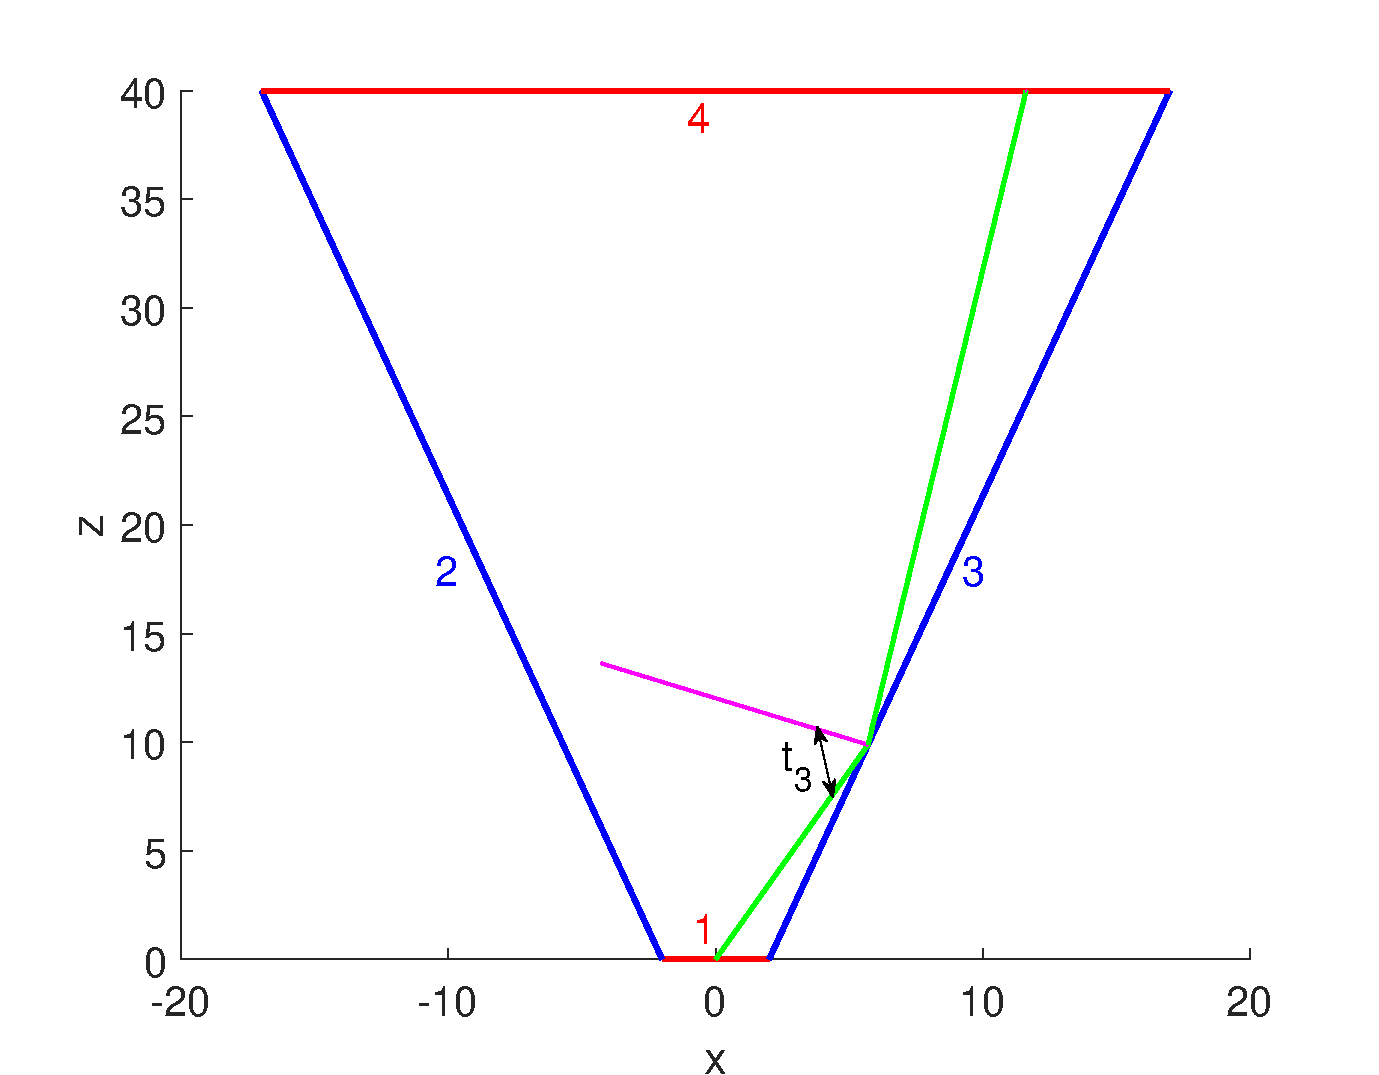
\includegraphics[width=6.7cm]{cup.pdf}
  \end{center}
  \caption{\footnotesize{Shape of the two-faceted cup.  Each line of the system is labeled with a number.
   The source \point{S}$= [-2,2]$ (line number $1$) is located on the $x$-axis.
   The target \point{T}$= [-17, 17]$ (line $4$) is parallel to the source and is located at a height $ z= 40$.
   The left and right reflectors (line $2$ and $3$) connect the source with the target.}}
  \label{figure:cup}
\end{figure}
\\ \indent The light source \point{S}$= [-\variabile{a}, \variabile{a}]$ (line $1$) and the target \point{T}$~=~ [-\variabile{b}, \variabile{b}]$ (line $4$) are two segments normal to the \variabile{z}-axis, where $\variabile{a}=2$ and $\variabile{b}=17$.
The left and right reflectors (line $2$ and $3$) are oblique segments that connect the source and the target.
All the optical lines \variabile{i} with $\variabile{i} \in \{1, \cdots, 4\}$ are located in air, therefore the refractive index $\variabile{n}_{\variabile{i}}=1$ for every \variabile{i}.
From now on, the coordinates $(\variabile{x}_{\variabile{i}}, \variabile{z}_{\variabile{i}})_{\variabile{i} =1, \cdots, 4}$ denote the intersection of the rays with line $\variabile{i}$ and,
$\vect{s}_\variabile{i}= (-\sin \variabile{t}_\variabile{i}, \cos \variabile{t}_\variabile{i})$ is the direction vector of the rays that leave $\variabile{i}$,
 with $\variabile{t}_\variabile{i}$ the angle that the ray forms with respect to the \variabile{z}-axis measured counterclockwise. As we consider only forward rays, the angles $\variabile{t}_\variabile{i}\in (-\pi/2, \pi/2)$.
 Therefore, a ray segment between $(\variabile{x}_\variabile{i}, \variabile{z}_\variabile{i})$ and $(\variabile{x}_\variabile{j}, \variabile{z}_\variabile{j})$ 
 with $\variabile{j}\neq\textit{i}$ is parameterized in real space by:
\begin{equation}
\label{parametrization}
\vect{r}(\variabile{s})=
\left( \begin{array}{cc}
\variabile{x}_\variabile{i}-\variabile{s}\sin(\variabile{t}_\variabile{i}) \\
\variabile{z}_\variabile{i}+\variabile{s}\cos(\variabile{t}_\variabile{i})\end{array} \right) \qquad \quad 0\leq \variabile{s}\leq \variabile{s}_{\textrm{max}}\,,
\end{equation}
where \variabile{s} denotes the arc-length and $\variabile{s}_{\textrm{max}}$ is the maximum value that it can assume.
\section{Monte Carlo ray tracing}


Assuming a Lambertian source, the input intensity at $\point{S}$ emitted in the direction $\variabile{t}_1$ is given by:
\begin{equation}\label{lambertian_source}
I(\variabile{t}_1) = 2\const{a}L\cos(\variabile{t}_1),
\end{equation}
where $L$ is the luminance and \variabile{a} is the half width of \point{S}.
In order to compute the target intensity, we need to find a relation between the intensities at \point{S} and \point{T}.
 Hence, we need to know how the optical system influences the direction of the rays when they hit an optical line.
 To this purpose, the ray tracing procedure is often used in optics.
Ray tracing relates the position coordinates
 $ (\variabile{x}_1, \variabile{z}_1)$ and the direction vector $\vect{s}_1$ of every ray at the source $\point{S}$ with the corresponding position $(\variabile{x}_4, \variabile{z}_4)$ and direction $\vect{s}_4$ at the target $\point{T}$. As in the following we will use often the target coordinates of the rays, from now on, to simplify the notation, we write $\variabile{t}$ instead of $\variabile{t}_4$ and $(\variabile{x}, \variabile{z})$ instead of $(\variabile{x}_4, \variabile{z}_4)$ for the target coordinates.\\ \indent The ray tracing algorithm can be schematized as follows.
 For every ray that leaves $\point{S}$ with initial position $(\variabile{x}_1, \variabile{z}_1)$ and initial angle $\variabile{t}_1$, its ray parametrization is implemented according to Eq. ($\ref{parametrization}$). Then, the coordinates $(\variabile{x}_\variabile{i}, \variabile{z}_\variabile{i})$ of the intersection point between the ray and the line $\variabile{i}$ that it hits are computed. The unit normal $\boldsymbol{\nu}_\variabile{i}$ to the line $\variabile{i}$ at the point $(\variabile{x}_{\variabile{i}}, \variabile{z}_{\variabile{i}})$ is calculated to compute the change of direction of the ray.
 Since all the lines of the system are located in air, only the reflection law plays a role, \cite{Hecht}.
 Therefore, denoting with $\vect{t}_1$ the direction of the incident ray, the direction $\vect{t}_2$ of the reflected ray is given by:
 \begin{equation}\label{reflection}
  \vect{t}_{2} = \vect{t}_1-2(\vect{t}_1,\boldsymbol{\nu}_{\variabile{i}})\boldsymbol{\nu}_{\variabile{i}}\,,
\end{equation}
where the vectors $\vect{t}_{1}$ and $\vect{t}_{2}$ are unit vectors, \cite{Chaves}.
The procedure explained above is repeated for every line that the ray encounters until it reaches the target and for every ray traced through the system. \\ \indent
There are different ways to implement the ray tracing procedure.
An often used method is MC ray tracing which calculates the target photometric variables considering a sample of many rays that are traced randomly from $\point{S}$ to $\point{T}$. The output intensity is computed as a function of the angular coordinate $\variabile{t}$ and is calculated dividing the target into intervals of the same length, the so-called bins. A partitioning $P_1: -\pi/2 = \variabile{t}_{0}<\variabile{t}_{1}<\cdots <\variabile{t}_{\const{Nb}}=\pi/2$ of the interval $[-\pi/2, \pi/2]$ is defined where $\const{Nb}$ is the number of bins in $P_1$.
We remark that, with a slight abuse of notation, we indicated the angular coordinates of the rays at the target with $\variabile{t}_{\variabile{j}}$ instead of $\variabile{t}_{4,\variabile{j}}$ for every $\variabile{j}\in\{0, \cdots, \const{Nb}\}$.
The normalized approximated intensity $g_{\const{MC}}(\variabile{t})$ is a piecewise constant function and its value over the $\variabile{j}$-th bin is the ratio between the number of rays that fall into that bin
$\const{Nr}[\variabile{t}_{\variabile{j}-1},\variabile{t}_{\variabile{j}})$ and the total number of rays traced $\const{Nr}[-\pi/2, \pi/2]$.
Hence, $g_{\const{MC}}$ is defined by:
\begin{equation} \label{g_mc}
g_{\const{MC}}(\variabile{t}) = \frac{\const{Nr}[\variabile{t}_{\variabile{j}-1},\variabile{t}_{\variabile{j}})}{\const{Nr}[-\pi/2, \pi/2]} \qquad \mbox{ for } \variabile{t}\in[\variabile{t}_{\variabile{j}-1}, \variabile{t}_{\variabile{j}}).
\end{equation}
Furthermore, the output intensity is computed from the value of the intensity $g_{\const{MC}}(\variabile{t}_{\variabile{j}-1/2})$ along the direction $\variabile{t}_{\variabile{j}-1/2}=(\variabile{t}_{\variabile{j}-1}+\variabile{t}_{\variabile{j}})/2$ for every bin $[\variabile{t}_{\variabile{j}-1},\variabile{t}_{\variabile{j}})_{\variabile{j} = 1, \cdots, \const{Nb}}$.
 The intensity $g_{\const{MC}}(\variabile{t}_{\variabile{j}-1/2})$ gives an estimate of the probability that a ray reaches the target with an angle in the $\variabile{j}$-th interval $[\variabile{t}_{\variabile{j}-1}, \variabile{t}_{\variabile{j}})$ of the partitioning $P_1$. This probability $\const{P}_{\variabile{j}, \Delta\variabile{t}}$ is given by:
\begin{equation}\label{eq:probability}
\const{P}_{\variabile{j}, \Delta\variabile{t}} = \Pr(\variabile{t}_{\variabile{j}-1}\leq\variabile{t}<\variabile{t}_{\variabile{j}})= \frac{\int_{\variabile{t}_{\variabile{j}-1}}^{\variabile{t}_{\variabile{j}}} G(\variabile{t}) \textrm{d}\variabile{t}}{\int_{-\pi/2}^{\pi/2}G(\variabile{t}) \textrm{d}\variabile{t}}\,,
\end{equation}
where $G(\variabile{t})$ is the output intensity (not normalized) and it is measured in lumen per radian $[lm/rad]$.
Note that $\sum_{\variabile{j}=1}^{\const{Nb}}\const{P}_{\variabile{j}, \Delta\variabile{t}}=1$. Using the mean value theorem for the function $G(\variabile{t})$ continuous in $[\variabile{t}_{\variabile{j}-1}, \variabile{t}_{\variabile{j}}]$, the integral at the numerator of the previous equation can be written as: \begin{equation}
\int_{\variabile{t}_{\variabile{j}-1}}^{\variabile{t}_{\variabile{j}}} G(\variabile{t}) \textrm{d}\variabile{t} = \Delta \variabile{t}\;G(\variabile{t}_{j-1/2}).
\end{equation}
Hence, $\const{P}_{\variabile{j}, \Delta\variabile{t}}$ is proportional to the size $\Delta\variabile{t}= (\variabile{t}_{\const{Nb}}-\variabile{t}_{0})/{\const{Nb}}$ of the intervals, i.e., inversely proportional to the number of bins $\const{Nb}$ of the partitioning $P_1$.
Indicating with $\Phi = \int_{-\pi/2}^{\pi/2}G(\variabile{t}) \textrm{d}\variabile{t}$ the total flux (measured in lumen $[lm]$),
the error between the intensity $G(\variabile{t}_{\variabile{j}-1/2})$
 and the averaged \const{MC} intensity $\Phi g_{\const{MC}}(\variabile{t}_{\variabile{j}-1/2})/\Delta\variabile{t}$ is given by:
\begin{equation}\label{eq:error_int}
\begin{aligned}
\Big|G(\variabile{t}_{\variabile{j}-1/2})&-\frac{\Phi}
{\Delta\variabile{t}}g_{\const{MC}}(\variabile{t}_{\variabile{j}-1/2})\Big| \leq\\
 &\Big|G(\variabile{t}_{\variabile{j}-1/2})-\frac{1}{\Delta \variabile{t}}\int_{\variabile{t}_{\variabile{j}-1}}^{\variabile{t}_{\variabile{j}}} G(\variabile{t})\textrm{d}\variabile{t}\Big|+\\
&\frac{1}{\Delta \variabile{t}}\Big|\int_{\variabile{t}_{\variabile{j}-1}}^{\variabile{t}_{\variabile{j}}} G(\variabile{t})\textrm{d}\variabile{t}-
\Phi\, g_{\const{MC}}(\variabile{t}_{\variabile{j}-1/2})\Big| \,.
\end{aligned}
\end{equation}
\indent The first term of the right hand side of inequality (\ref{eq:error_int}) gives an estimate of how much the averaged intensity $\frac{1}{\Delta \variabile{t}}\int_{\variabile{t}_{\variabile{j}-1}}^{\variabile{t}_{\variabile{j}}} G(\variabile{t})\textrm{d}\variabile{t}$ differs from the exact intensity $G(\variabile{t}_{\variabile{j}-1/2})$.
This term is due to the discretization of the target and therefore it depends on the number of bins $\const{Nb}$ considered.
  Substituting $G(\variabile{t})$ with its Taylor expansion around the point $\variabile{t}_{\variabile{j}-1/2}$ we obtain that this term is proportional to the square of the size of the bins, therefore the following equality holds:
\begin{equation}\Big|G(\variabile{t}_{\variabile{j}-1/2})-\frac{1}{\Delta \variabile{t}}\int_{\variabile{t}_{\variabile{j}-1}}^{\variabile{t}_{\variabile{j}}} G(\variabile{t})\textrm{d}\variabile{t}\Big| = \const{C}_1/\const{Nb}^2\end{equation}
with $C_1>0$ a certain constant. \\
\indent
The second part of the right hand side of inequality (\ref{eq:error_int}) gives an estimate of the MC error and therefore it depends also on the
number of rays traced.
In order to show how this term decreases as a function of the number of rays traced,
we define the random variable $\variabile{X}_\variabile{j}(\variabile{t})$ as the variable that is equal to $1$ if the ray with angular coordinate $\variabile{t}$
is inside the interval $[\variabile{t}_{\variabile{j}-1}, \variabile{t}_{\variabile{j}})$ and equal to $0$ otherwise,
\begin{equation}
\label{radom_variable}
\variabile{X}_{\variabile{j}}(\variabile{t}) = \begin{cases} \begin{aligned}
1& \qquad \mbox{if} \quad \variabile{t}\in [\variabile{t}_{\variabile{j}-1}, \variabile{t}_{\variabile{j}}),\\
0 & \qquad \mbox{otherwise}.
\end{aligned}\end{cases}
\end{equation}
The Bernoulli trial $ \variabile{X}_{\variabile{j}}$ follows a binomial distribution $B(1,\const{P}_{\variabile{j}, \Delta\variabile{t}})$.
Considering a sample of $\const{Nr}$ rays, the variable $\variabile{Y}_{\variabile{j}} = \sum_{\variabile{k}=1}^{\const{Nr}} \variabile{X}_{\variabile{j}}(\variabile{t}_{\variabile{k}})$
follows a binomial distribution $B(\const{Nr}, \const{P}_{\variabile{j},\Delta \variabile{t}})$, where $\variabile{t}_{\variabile{k}}$ is the angle that the $\variabile{k}$-th ray forms with the optical axis. Then, using the de Moivre-Laplace theorem, we conclude that the variable $\variabile{Y}_{\variabile{j}}$ is approximated by a normal distribution with mean value $\variabile{E}[\variabile{Y}_{\variabile{j}}] = \const{Nr}\const{P}_{\variabile{j}, \Delta\variabile{t}}$ and variance $\sigma^2[\variabile{Y}_{\variabile{j}}] = \const{Nr}\const{P}_{\variabile{j}, \Delta\variabile{t}}(1~-~\const{P}_{\variabile{j}, \Delta\variabile{t}})$ when a large number of rays is considered, see \cite{Rubinstein, deMoivre}.
Thus, the normalized intensity along the direction $\variabile{t}_{\variabile{j}-1/2}$ is given by:
\begin{equation}\variabile{g}_{\const{MC}}(\variabile{t}_{\variabile{j}-1/2}) = \sum_{\variabile{k}=1}^{\const{Nr}}\variabile{X}_{\variabile{j}}(\variabile{t}_{\variabile{k}})/\const{Nr}.\end{equation}
The mean value $E[\variabile{g}_{\const{MC}}(\variabile{t}_{\variabile{j}-1/2})]=\const{P}_{\variabile{j}, \Delta\variabile{t}}$
and the variance $\sigma^2[\variabile{g}_{\const{MC}}(\variabile{t}_{\variabile{j}-1/2})] ~=~ \const{P}_{\variabile{j}, \Delta\variabile{t}}(1-\const{P}_{\variabile{j}, \Delta\variabile{t}})/\const{Nr}$.
Note that the standard deviation $\sigma_\variabile{j}:=\sigma[\variabile{g}_{\const{MC}}(\variabile{t}_{\variabile{j}-1/2})]$ equals:
\begin{equation}\label{sigma}
\sigma_\variabile{j}= \sqrt{\const{P}_{\variabile{j}, \Delta\variabile{t}}(1-\const{P}_{\variabile{j}, \Delta\variabile{t}})/\const{Nr}}= \frac{\const{C}_2}{\sqrt{\const{Nb}\const{Nr}}}\,, \end{equation}
 for some $\const{C}_{2}>0$. $\sigma_\variabile{j}$ can be used to give an estimate of the difference between the intensity $\variabile{g}_{\const{MC}}(\variabile{t}_{\variabile{j}-1/2})$ and its mean value $\const{P}_{\variabile{j}, \Delta\variabile{t}}$.
Therefore, the second term of the right hand side of relation ($\ref{eq:error_int}$) becomes:
\begin{equation}\begin{aligned}
\frac{1}{\Delta \variabile{t}}\Big|\int_{\variabile{t}_{\variabile{j}-1}}^{\variabile{t}_{\variabile{j}}} G(\variabile{t})\textrm{d}\variabile{t} -
\Phi\, g_{\const{MC}}(\variabile{t}_{\variabile{j}-1/2})\Big| &=  \\
\frac{\Phi}{\Delta \variabile{t}}\Big|\const{P}_{\variabile{j}, \Delta\variabile{t}} -g_{\const{MC}}(\variabile{t}_{\variabile{j}-1/2})\Big| &\propto  \\
  \frac{\Phi}{\Delta \variabile{t}}
\sigma_{\variabile{j}}[\variabile{g}_{\const{MC}}(\variabile{t}_{\variabile{j}-1/2})]=\const{C}_3\frac{\const{Nb}}{\sqrt{\const{Nb}\const{Nr}}} & = \const{C}_3\sqrt{\frac{\const{Nb}}{\const{Nr}}}\,,
\end{aligned}
\end{equation}
for some $\const{C}_3>0$, where the approximation holds because $\sigma_{\variabile{j}}$ gives a measure for the error between $g_{\const{MC}}(\variabile{t}_{\variabile{j}-1/2})$ and the probability $\const{P}_{\variabile{j}, \Delta\variabile{t}}$, \cite{Diez}. The second equality follows from Eq. (\ref{sigma}). To conclude, the MC error over the $\variabile{j}$-th bin is estimated by:
\begin{equation} \begin{aligned}
\Big|G(\variabile{t}_{\variabile{j}-1/2})&-\frac{\Phi}
{\Delta\variabile{t}}g_{\const{MC}}(\variabile{t}_{\variabile{j}-1/2})\Big| =
\frac{\const{C}_1}{\const{Nb}^2} + \const{C}_4\sqrt{\frac{\const{Nb}}{\const{Nr}}},
\end{aligned}
\end{equation}
for $\const{C}_4>0$.
Considering a fixed number of rays, we obtain that the minimal error is reached when $\const{Nb}\approx \const{Nr}^{1/5}$.
Hence, if $10^{10}$ rays are considered the target has to be divided into $10^2$ bins to minimize the MC error.
This leads to computational efforts resulting in a very slow procedure.





To obtain the photometric variables at the target, the propagation of light from the source $\mathcal{S}$ to the target $\mathcal{T}$ is computed.
In this work, we calculate the output intensity for the TIR-collimator, the profile of which is depicted in Figure $\ref{fig:analyticlens}$.
\begin{figure}[t]
  \begin{center}
  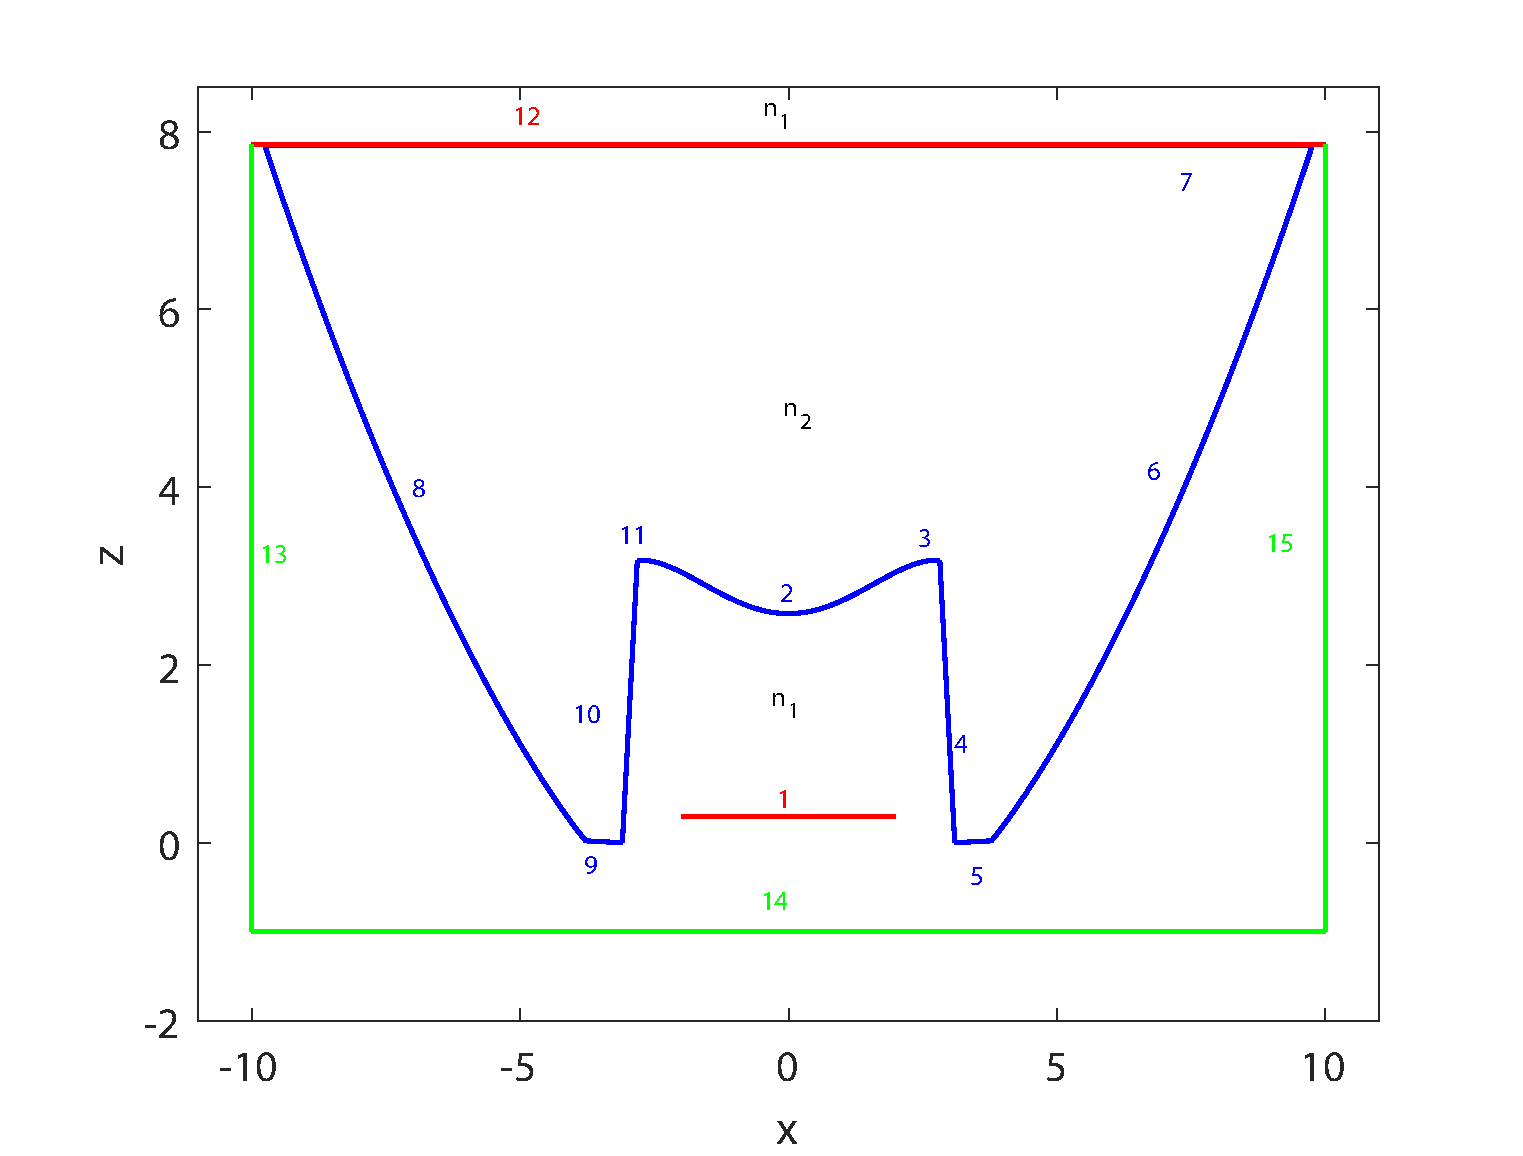
\includegraphics[width=6.5cm]{tir_analytic2.pdf}
   \end{center}
    \caption{\footnotesize{Shape of the TIR-collimator. Each line of the system is labeled with a number.
       The source $\mathcal{S}= [-2,2]$ (line number $1$) is located at an height $z_{\textrm{s}} = 0.3$ from the $x$-axis.
       The target $\mathcal{T}= [-9.7, 9.7]$ (line $12$) is parallel to the source and is located at an height $ z_{\textrm{t}}= 7.85$.
       The shape of the collimator is shown as a blue line.
       Three detectors depicted with green lines (lines $13$, $14$, and $15$) are located at the left, the right and the bottom of the optical system.
       $n_1 = 1$ is the refraction index of the medium (air) where the source and the target are located, and
       $n_2 = 1.5 $ the refraction index of the medium (glass) inside the optical system. The sagitta of the lens is equal to $0.6$.}}
 \label{fig:analyticlens}
\end{figure}
\\
The TIR-collimator we analyze is an optical system rotationally symmetric with respect to the $z$-axis and consists of a lens (line $2$), two broken lines adjacent to the lens (formed by the collection of the segments $3, 4, \mbox{ and } 5$ and $9, 10 \mbox{ and } 11$),
two curved lines (labeled with $6$ and $8$) and the top formed by a horizontal segment (line $7$). The lens and the broken lines are refractive lines while, the curved lines are designed in such a way that light is internally reflected (which explains the name TIR).
The light source $\mathcal{S}$ (line $1$) and the target $\mathcal{T}$ (line $12$) are two straight segments normal to the optical axis and are located in air ($n_1=1$) while
the volume inside the collimator is filled with a material with index of refraction $n_2=1.5$ (e.g. glass).
The collimator is surrounded by two vertical and two horizontal lines (lines $13$, $15$, $12$ and $14$, respectively) that receive the light exiting from the optical system; among these, the horizontal one at the top is assumed to be the light target and, it is located at a small distance from the top. \\
\indent From now on, the coordinates $(x_{\textit{i}}, z_{\textit{i}})_{(i =1, \cdots, 15)}$ denote the intersection of the rays with the line $\textit{i}$ and, $\textbf{s}_\textit{i}= (-\sin t_\textit{i}, \cos t_\textit{i})$ is the direction vector of the rays that leave the line $\textit{i}$, where $t_\textit{i}~\in~ (-\pi/2, \pi/2)$ is the angle
 that the ray forms with the $z$-axis, measured counterclockwise.
 Therefore, a ray segment between $(x_\textit{i}, z_\textit{i})$ and $(x_\textit{i+1}, z_\textit{i+1})$ is parameterized by:
\begin{equation}
\label{parametrization}
\textbf{r}(s)=\begin{pmatrix}x_\textit{i}-s\sin(t_\textit{i})\\ z_\textit{i}+s\cos(t_\textit{i})\end{pmatrix}  \qquad \quad s\geq 0\,,
\end{equation}
where $s$ denotes the arc-length.
\\  \indent A Lambertian optical source is considered; hence, the intensity over an interval $J ~=~ [-a, a]$ emitted in the direction $t$ is given by:
\begin{equation}
\label{lambertian_source}
I(t) = I_0\cos(t),
\end{equation}
where $I_0= 2aL$, $L$ is the luminance, and $t$ is the angle that the ray forms with respect to the optical axis, measured counterclockwise.
As a result, in the case where $L=1$, $I_0$ coincides with the source length; from Equation ($\ref{lambertian_source}$), the intensity at the source is deduced. \\
\indent To compute the target intensity, we need to know how the optical system changes the direction of the rays during their propagation from the source to the target.
To do this, we employ the ray tracing technique which can be summarized as follows: first, a ray from the source with initial position given by the coordinates $(x_1, z_1)$ and initial angle $t_1$ with respect to the $z$- axis is traced and, the ray parametrization is implemented according to Equation ($\ref{parametrization}$). Second, the intersection point $(x_\textit{i}, z_\textit{i})$ between the ray and the line $\textit{i}$ that it hits first is computed. Third, the normal to the line hit at the point $(x_{\textit{i}}, z_{\textrm{i}})$ is calculated to compute the change of direction of the ray.
For the last step, the laws of reflection and refraction are implemented.
The direction of the refractive ray is given by:
\begin{equation}\label{refraction}
\textbf{t}=n_{1,2}\,\textbf{i}+\Big[\sqrt{1-n_{1,2}^2+n_{1,2}^2(\textbf{n},\textbf{i})^2}-n_{1,2}(\textbf{n},\textbf{i}) \Big]\textbf{n}\,,
\end{equation}
where $n_{1,2}=n_1/n_2$ with $n_1$ and $n_2$ the refraction indexes of air and of glass, respectively.
The unit vectors $\textbf{i}$ and $\textbf{t}$ describe the directions of the incident and refracted ray, respectively; $\textbf{n}$ is the normal to the line; it is also a unit vector and it is directed towards the interior of the optical system.
Note that the positive sign before the square root is due to the convention to take the inward direction of the normal $\textbf{n}$ (see \cite{hecht1998hecht}, chapter 4, p. 95-106, and, \cite{chaves2008introduction}, chapter 12 p. 403-409).
In the case where $n_1 = -n_2$, Equation (\ref{refraction}) can be rewritten as the law of reflection:
\begin{equation}\label{reflection}
\textbf{t} = \textbf{i}-2(\textbf{i}, \textbf{n})\textbf{n}.
\end{equation}
Equation ($\ref{reflection}$) is used when the total internal reflection condition holds, that is when the following inequality is true:
\begin{equation}\label{eq: Tir-condition}
1-n_{1,2}^2+(\textbf{n},\textbf{i})^2<0\,.
\end{equation}
For the TIR-collimator the previous condition occurs for the curved lines (lines $6$ and $8$ in Figure \ref{fig:analyticlens}).
Finally, the new parametrization of the ray is described by:
\begin{equation}
\textbf{r}(s)=
\begin{pmatrix}
x_i+s\,t_{x} \\ z_i+s\,t_{z}
\end{pmatrix}\,,
\end{equation}
where
$t_{x}$ and $t_{z}$ are the $x$ and $z$-components of the new ray direction and are calculated from Equations ($\ref{refraction}$) or ($\ref{reflection}$).
The points $(x_\textit{i}, z_\textit{i})$ and the new direction $\textbf{t}$ are computed until the ray hits the target and the previous procedure is repeated for each ray traced. \\
\indent To obtain a reasonable approximation of the target intensity, a large number of rays has to be traced; the more rays are traced, the more accurate the target intensity is.
Moreover, for the TIR-collimator shown in Figure $\ref{fig:analyticlens}$, we do not have an explicit equation to describe the reflectors. Only the positions of a discrete set of points located on their curves are known.
Therefore, we use spline interpolation to obtain a good approximation of the curved lines. In addition, to calculate the intersection points between the rays and these lines, the Newton-Raphson procedure is employed. Due to all these reasons, the ray-tracing method is a very slow procedure.\\
\indent A frequently used ray tracing method in non-imaging optics is MC ray tracing \cite{Ting:1} in which the rays are emitted from a random location and at random angle. They are traced through the system until they reach the target receiver. To calculate the output intensity, the target screen is divided into bins and the frequency of the rays that arrive at each bin is considered. The intensity restricted to a certain bin is obtained by dividing the number of rays that fall into that bin by the total number of rays traced.
Although MC ray tracing is highly robust and does not require difficult calculations, it has two main disadvantages.
First, some information is lost because the flux of a ray is averaged over a bin.
Second, some parts of the target are reached by a very small fraction of rays and, consequently, the intensity is unreliable in those parts.
As a consequence, a large number of rays needs to be traced to obtain an accurate intensity making the MC method computationally expensive.
\\
\indent We provide a new method that employs the phase space representation of the optical system to avoid tracing rays where the luminance does not present any discontinuities.
Phase space ray tracing is explained in the next section.

In phase space each ray is described by its intersection point with the line it hits and the sine of the angle it forms with respect to the optical axis multiplied by the refractive index (see \cite{wolf2004geometric} chapter 2.1-2.3, \cite{rausch2014phase}, and \cite{torre2005linear} chapter 1 for details).
In the following, the phase space is considered only for the source $\mathcal{S}$ and the target $\mathcal{T}$ and for no other line of the optical system.
The rays in a two-dimensional system correspond to points with coordinates $(x,\tau)$ and $(q,\eta)$ in $\mathcal{S}$ and $\mathcal{T}$ phase space, respectively.
We have indicated the ray positions with $x$ and $q$, the angles formed with the normal with $t$ and $\theta$, the refractive indexes with $n_{\textrm{s}}$ and $n_{\textrm{t}}$, for $\mathcal{S}$ and $\mathcal{T}$, respectively and, with $\tau = n_{\textrm{s}}\sin(t)$ and $\eta = n_{\textrm{t}}\sin(\theta)$ the directions of the rays.

The rays are represented by a unique point in phase space, both for $\mathcal{S}$ and $\mathcal{T}$.
More formally, the optical phase space for the light source is defined as: \begin{equation}
\mathcal{P}_\textrm{s}=\mathcal{S}\times[-n_\textrm{s},n_\textrm{s}] .\end{equation}
The target phase space is defined as \begin{equation}\mathcal{P}_\textrm{t}=\mathcal{T}\times[-n_\textrm{t},n_\textrm{t}] .\end{equation}
The map $\mathcal{M}:\mathcal{P}_{\textrm{s}}\rightarrow\mathcal{P}_{\textrm{t}}$ which describes how the optical system changes the rays is defined as:
\begin{equation}\label{M}
\mathcal{M}(x,\tau)=(q,\eta).
\end{equation}
For most optical systems, there is no way to determine an explicit expression for the map $\mathcal{M}$ defined above.
The idea is to apply the edge-ray principle \cite{Ries:2} to a given set of rays at the source.
The principle states that to map one region from the source to the target phase space it is sufficient to map the boundaries of those regions.
Therefore, the boundaries of the source are mapped to the boundaries of the target and the regions where the luminance is different from zero are calculated.
The intensity in target phase space is defined as a function of the output luminance:
\begin{equation}\label{I(eta)}
I_{PS}(\eta) = \int_{\mathcal{T}_{\eta}} L_{\textrm{t}}(q, \eta) dq  \,,
\end{equation}
where, for a given constant $\eta_0 \in [-1,1]$, the set $\mathcal{T}_{\eta_0}~=~\{(q, \eta)~\in~ \mathcal{T}\:|\: \eta ~=~ \eta_0 \}$ and $L_{\textrm{t}}(q, \eta)$ indicates the luminance at the target.
As we use the target phase space to compute the output intensity, it is convenient to define it as a function of $\sin(\theta)$ instead of $\theta$.
Note that the luminance is positive in the entire $\mathcal{P}_\textrm{s}$, but not all parts of $\mathcal{P}_\textrm{t}$ receive light emitted by the source.
As a result, $L_\textrm{t}$ has jump discontinuities where it changes from zero to positive values.
To understand where these discontinuities occur, further information about the rays is required.
Because of this, for PS ray tracing not only the initial positions and the initial angles of the rays are stored,
 but also the optical lines they hit when they propagate through the system.
A ray path $\Pi$ is defined as the collection of lines hit by the ray. %that the rays hit when propagate through the optical system.
Rays that are close to each other at the source and leave the source at close angles follow the same path and hit the target at close positions and under close angles.
All the rays that follow the same path are grouped together into the same subset of phase space.
 From now on, we indicate with $p$ the number of all the possible paths $(\Pi_{j})_{j = 1, \cdots, p}$ encountered by the rays
  and, with $R_{\textrm{s}, \Pi_j}$ and $R_{\textrm{t}, \Pi_j}$ the regions corresponding to the rays that follow the path $\Pi_j$ for the source and the target, respectively.
  The map $\mathcal{M}$ defined in Equation (\ref{M}) relates the regions $R_{\textrm{s}, \Pi_j}$ to the regions $R_{\textrm{t}, \Pi_j}$ for every $j \in \{1, \cdots,p \}$.
The edge-ray principle guarantees that the boundaries $\partial R_{\textrm{s}, \Pi_j}$ and $\partial R_{\textrm{t}, \Pi_j}$ are connected by the same map $\mathcal{M}$.
Given two different paths $\Pi_1$ and $\Pi_2$, the regions $R_{\textrm{t}, \Pi_1}$ and $R_{\textrm{t}, \Pi_2}$ do not overlap; they can have at most a common boundary.
As a result, the discontinuities of the luminance occur exactly at the boundaries $(\partial R_{\textrm{t}, \Pi_j})_{j = 1,\cdots, p}$.
Finally, the luminance at the target satisfies the following relations:
\begin{equation}
\begin{array}{cc}
\begin{aligned}
 \label{luminance}
L_\textrm{t}(q, \eta) &> 0  &\qquad \mbox{ for } (q, \eta)\in (R_{\textrm{t}, \Pi_j})_{j = 1, \cdots, p}, \\
L_\textrm{t}(q, \eta) &= 0 &\mbox{otherwise}. \qquad \qquad \qquad \;\;\,
\end{aligned}
\end{array}
\end{equation}
In addition, the luminance is conserved along a ray, so it remains constant inside every region $ (R_{\textrm{t}, \Pi_j})_{j  =1, \cdots, p }$, (see \cite{chaves2008introduction}, chapter 16).
The output intensity is obtained from Equation ($\ref{I(eta)}$).
Therefore, the problem to compute the target intensity can be interpreted as the calculation of the boundaries $(\partial R_{\textrm{t}, \Pi_j})_{j = 1,\cdots, p}$.
To this end, we define a triangulation on source phase space in such a way that more rays close to the boundaries are traced.
The details of these procedures are explained in the next section.

\subsection{Triangulation refinement of source phase space} \label{subsec:triangulation1}
The regions $(R_{\textrm{t}, \Pi_j})_{j =1, \cdots, p}$ can be defined only when some rays are traced.
Given an initial set of rays, the rays closest to the boundaries $(\partial R_{\textrm{t}, \Pi_j})_{j = 1, \cdots, p}$ are selected and more rays in their vicinity are created to get progressively better estimates of the boundaries. A more detailed description is provided below.
A triangulation in $\mathcal{P}_\textrm{s}$ is defined and a ray from every vertex $(x_k, \tau_k)$ of the triangle is traced.
The procedure starts tracing four rays with coordinates $(x_k,\tau_k)_{k=1, \cdots, 4}$ that are located exactly at the corners of $\mathcal{P}_\textrm{s}$ and, for each of them, the paths $(\Pi_{j})_{j = 1, \cdots, 4}$, are stored. Next, for some $j \in\{1, \cdots, 4\}$, the grid is divided into two equal triangles joining two opposite vertices. For each triangle the rays located at its corners are traced. If the paths corresponding to
those rays are different, one or more boundaries
$(\partial R_{\textrm{t}, \Pi_j})_{j =1, \cdots, 4}$ are expected to cross the triangle.
In that case, the middle points $(x_k, \tau_k)_{k = 5, 6, 7}$ of each side of the triangle are added and
three more rays with coordinates $(x_k, \tau_k)_{k = 5, 6,7}$ are traced. Each refinement step leads to four new triangles (see Figure \ref{fig:refinement}).
 \begin{figure}[t]
  \begin{center}
  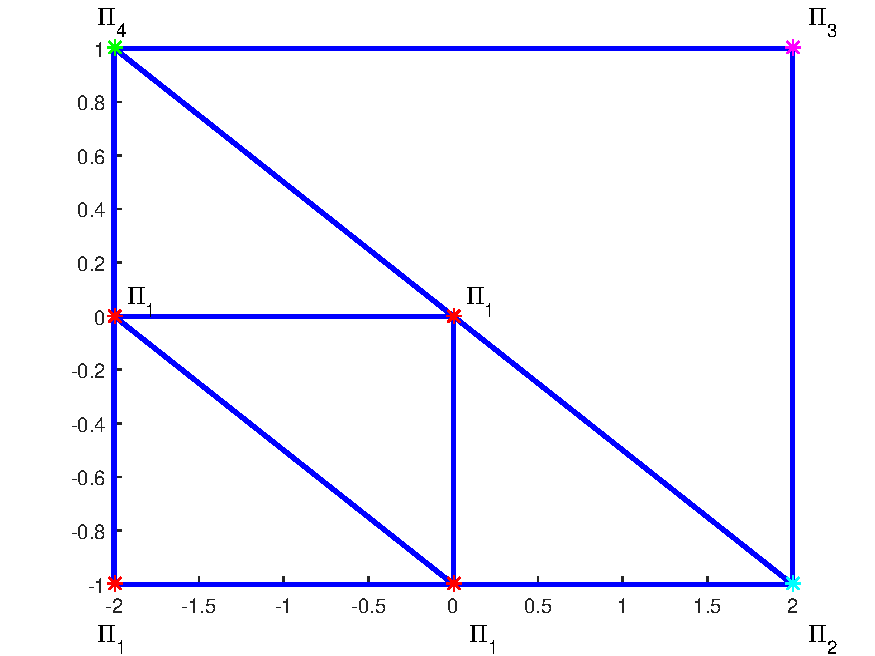
\includegraphics[width=5.7cm]{grid.pdf}
  \end{center}
  \caption{\footnotesize{Triangulation refinement:
  when the rays related to the vertices of the triangles follow a different path a new refinement step is required.
   Each refinement step leads to four new triangles.
   The parameters values are $\epsilon_{x_{max}}~=~ 2$, $\epsilon_{\tau_{max}}= 1$, $\epsilon_{x_{min}}= 4$ and $\epsilon_{\tau_{min}}=2$.   }}
  \label{fig:refinement}
\end{figure}
  \\
 \indent
When all the rays in the corners of each triangle have the same path, it is not necessary to refine the triangles anymore.
\noindent Note that it can happen that a region formed by rays that follow a path $\Pi_j$ is located completely inside a triangle whose vertices are related to the same path $\Pi_i$ with $j \neq i$. In that case the algorithm is not able to detect that region, see Figure \ref{fig:region inside}. To avoid this, two parameters $\epsilon_{x_{min}}$ and $\epsilon_{\tau_{min}}$ are defined for the $x$-axis and the $\tau$-axis, respectively. When the length of the sides of the triangle are greater than these parameters, a new triangle is defined even if its vertices correspond to the same path. Furthermore, two other parameters $\epsilon_{x_{max}}$ and $\epsilon_{\tau_{max}}$ are introduced to defined a stopping criterion.
The algorithm stops when the length of the sides of the triangles is smaller than $\epsilon_{x_{max}}$ and $\epsilon_{\tau_{max}}$.
\begin{figure}[t]
  \begin{center}
  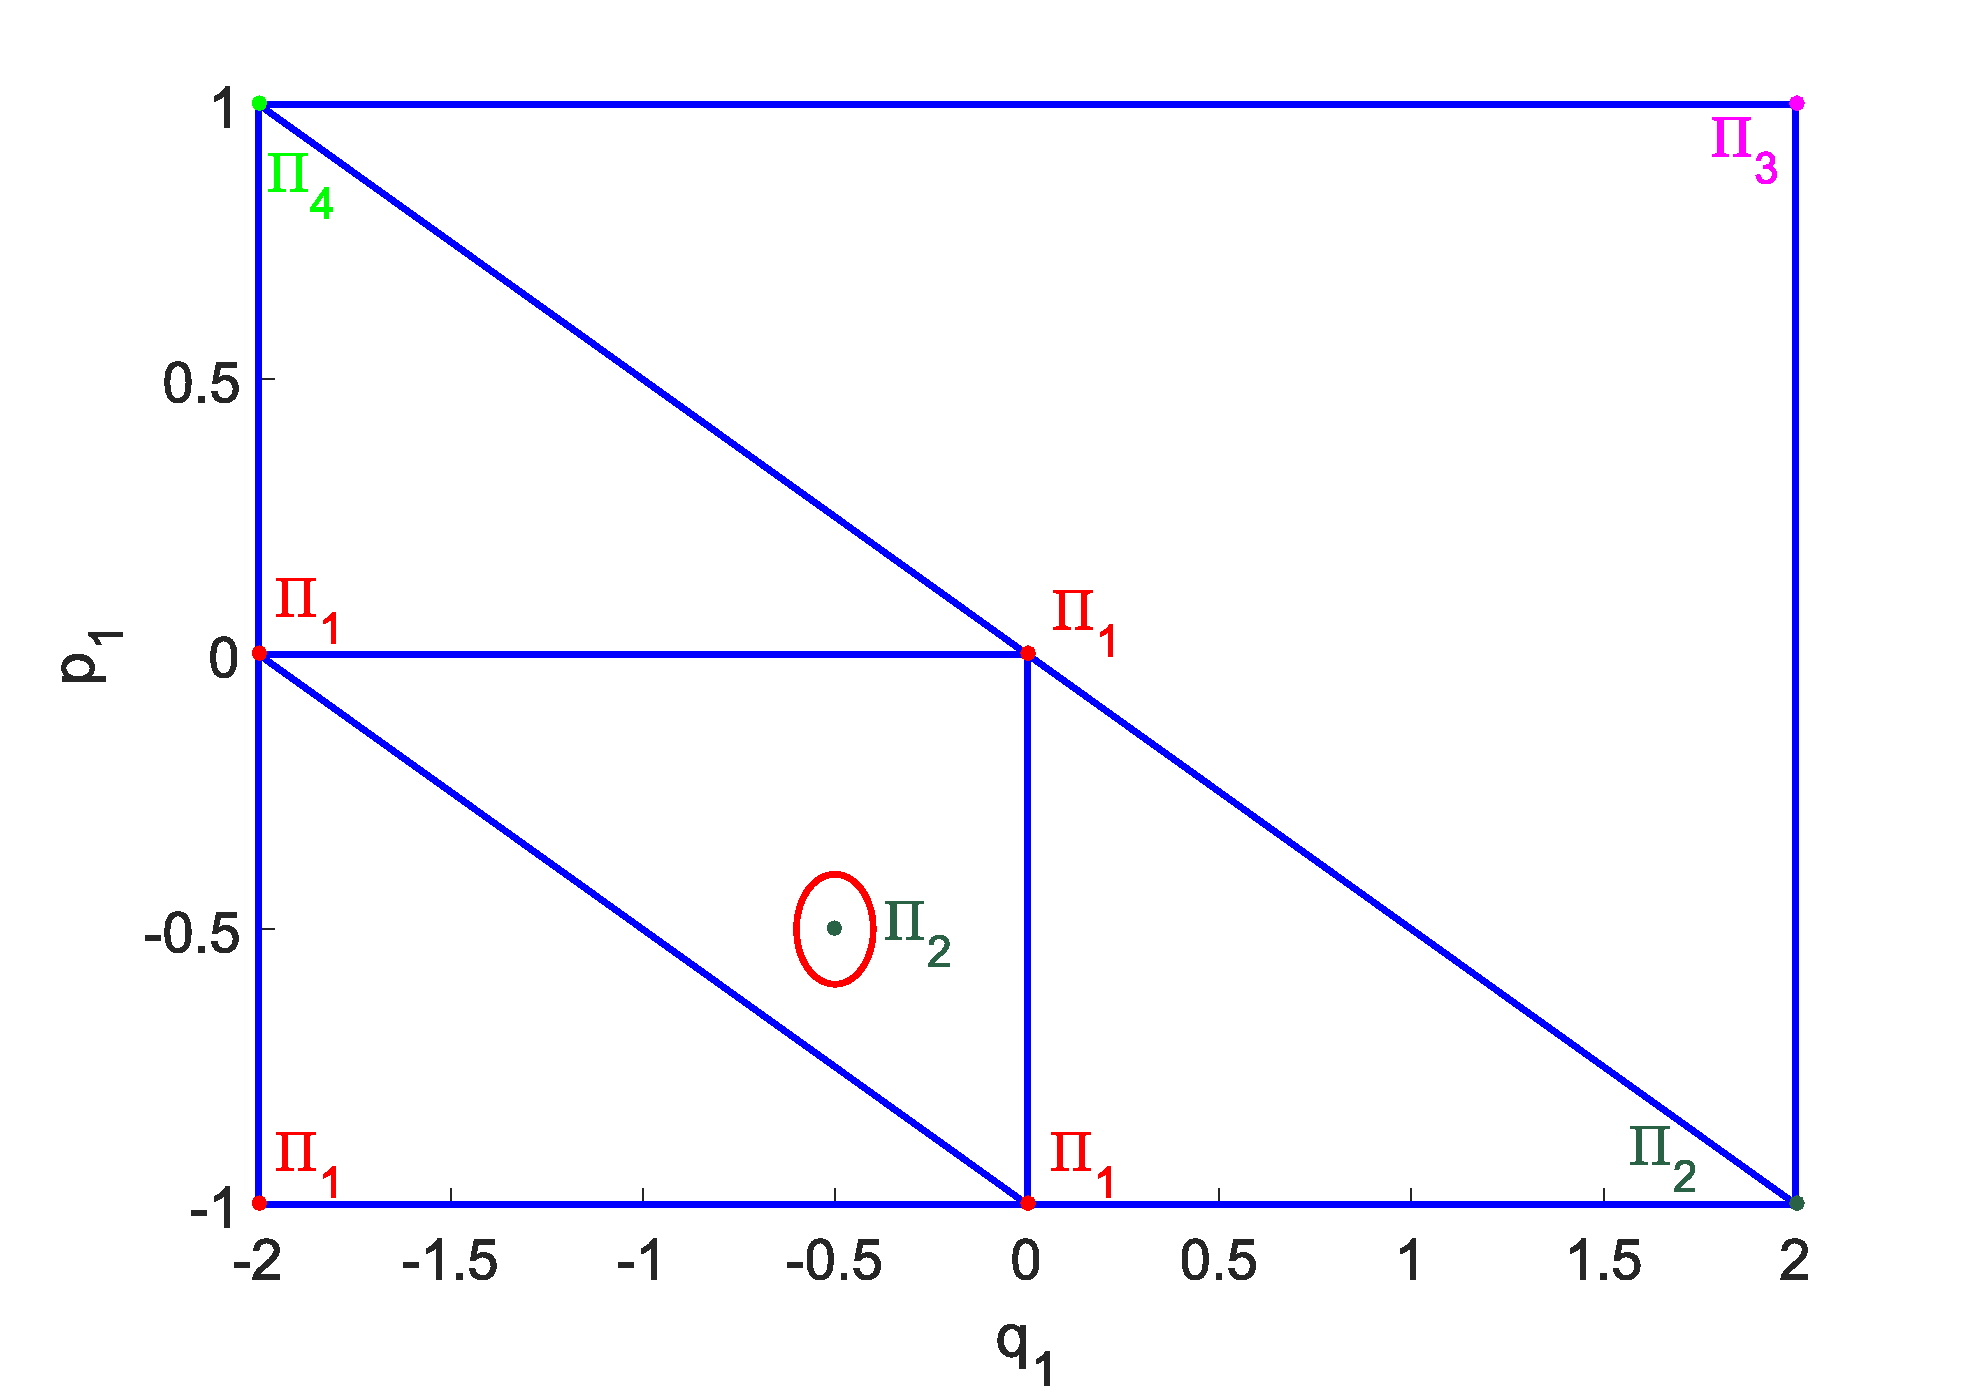
\includegraphics[width=5.5cm]{region_inside.pdf}
  \end{center}
  \caption{\footnotesize{The red line encloses a region of rays that follow the path $\Pi_2$ and is completely located inside a triangle.
  The algorithm is not able to detect that region and, a further refinement is required.
    The parameters values are $\epsilon_{x_{max}}~=~ 2$, $\epsilon_{\tau_{max}}= 1$, $\epsilon_{x_{min}}= 4$ and $\epsilon_{\tau_{min}}=2$. }}
   \label{fig:region inside}
  \end{figure}
The values of the parameters $\epsilon_{x_{max}}$, $\epsilon_{\tau_{max}}$, $\epsilon_{x_{min}}$ and $\epsilon_{\tau_{min}}$ determine the number of rays traced.
Indeed, on the one hand, $\epsilon_{x_{max}}$ and $\epsilon_{\tau_{max}}$ can be decreased to obtain more rays close to the boundaries;
on the other hand, a large number of rays in the interior of the regions can be traced decreasing the values of $\epsilon_{x_{min}}$ and $\epsilon_{\tau_{min}}$. %
\newline
\indent Using the above procedure, rays increasingly closer to the boundaries are traced.
For our optical system, the width of the $x$-axis in source phase space is two times the width of the $\tau$-axis.
Thus, our choice is $\epsilon_{\tau_{min}}=\frac{1}{2}\epsilon_{x_{min}}$ and $\epsilon_{\tau_{max}} = \frac{1}{2}\epsilon_{x_{max}}$.
Figure \ref{fig:triangulation_refinement} shows an example of a triangulation refinement of the source phase space with $\epsilon_{x_{max}}=0.1$ and $\epsilon_{x_{min}}=1$.
The triangulation refinement provides more triangles close to the boundaries $\partial R_{\textrm{s}, \Pi_j}$ than those inside the regions $R_{\textrm{s}, \Pi_j}$.
\begin{figure}[h]
  \begin{center}
  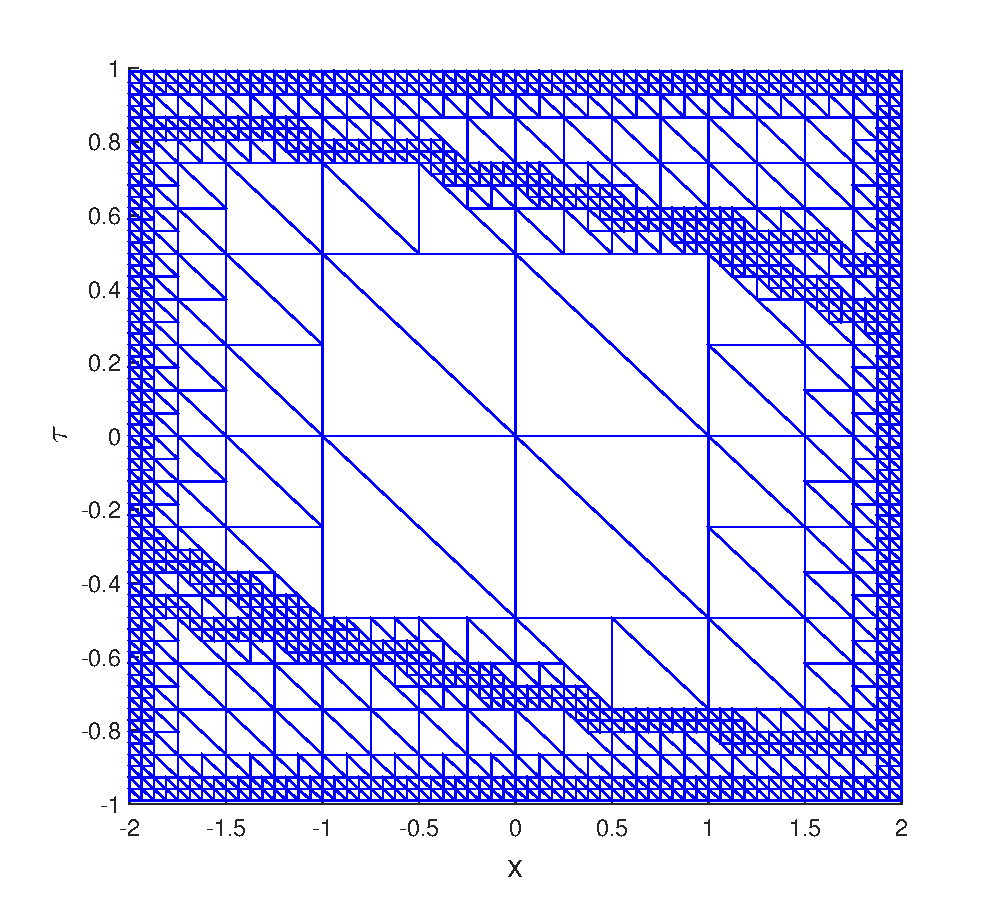
\includegraphics[width=5.7cm]{triangulation_refinement1.pdf}
  \end{center}
  \caption{\footnotesize{Triangulation refinement of source phase space:
  near the boundaries more rays are traced.
    The values of the parameters are $\epsilon_{x_{max}}~=~ 0.1$ and $\epsilon_{x_{min}}~=~1$.}}
   \label{fig:triangulation_refinement}
  \end{figure}
 \\ \indent The paths $(\Pi_j)_{j = 1, \cdots, p}$ followed by the rays located at the corner of the triangles are computed during the procedure and, the regions
 $R_{\textrm{s}, \Pi_j}$ and $R_{\textrm{t}, \Pi_j}$ are defined for each $\Pi_j$.
Next, a criterion to select the values of the parameters $\epsilon_{x_{min}}$ and $\epsilon_{x_{max}}$ and a method to compute the boundaries $\partial{R_{t, \Pi_j}}$ is provided.
Furthermore, the output photometric variables are computed, the details are explained in the next section.
As mentioned in Section \ref{sec:method}\ref{subsec:phasespace}, the boundaries $(\partial R_{\textrm{t}, \Pi_j})_{j = 1,\cdots, p}$ have to be calculated to compute the photometric variables at the target. Our method is based on the triangulation refinement of the source phase space.
More rays close to the boundaries can be traced selecting increasingly smaller values for the parameters $\epsilon_{x_{max}}$ and $\epsilon_{\tau_{max}}$. Once the algorithm stops, only the triangles that are expected to be crossed by a boundary are taken into account.
By construction, each of these triangles has two vertices that follow the same path and one vertex that follows another path.
The triangles are ordered in such a way that two of them are neighbors if they have a side in common. Given a path $\Pi_j$ with $j \in \{1, \cdots, p\}$ the boundary $\partial R_{\textrm{s}, \Pi_j}$ of the region corresponding to $\Pi_j$ is approximated by those vertices of the triangles corresponding to the path $\Pi_j$.
The boundaries $\partial R_{t, \Pi_j}$ at the target are given by $\mathcal{M}(\partial R_{s, \Pi_j})$ for every $j \in \{1, \cdots, p \}$.
To establish the minimum value of the parameter $\epsilon_{x_{max}}$ that gives a good approximation of the boundaries $\partial R_{\textrm{t}, \Pi_j}$,
a technique that exploits the conservation of the \'{e}tendue in phase space is provided, (see \cite{chaves2008introduction}, chapter 16). The essence of our approach is as follows.\\
\indent We consider the \'{e}tendue for the whole $\mathcal{P}_\textrm{s}$ which is given by:
\begin{equation}\label{etenduesource}
E_{\textrm{s}} = 2n_{\textrm{s}} a \sin(t_{max})\,,
\end{equation}
 where $a$ is the length of the source  and $t_{max}$ is the maximum value of the angle that the rays make with the $z$-axis.
 The \'{e}tendue of a set of rays is defined by the area they occupy in phase space.
 For the TIR-collimator we considered (Figure \ref{fig:analyticlens}), the area of $\mathcal{P}_\textrm{s}$ is equal to $7.92$, as $a = 4$ and $\sin(t_{max}) ~=~ 0.99$.
 The rays traced are uniformly distributed over $\mathcal{P}_\textrm{s}$, and they cover it entirely.
 \begin{figure}[h]
  \begin{center}
  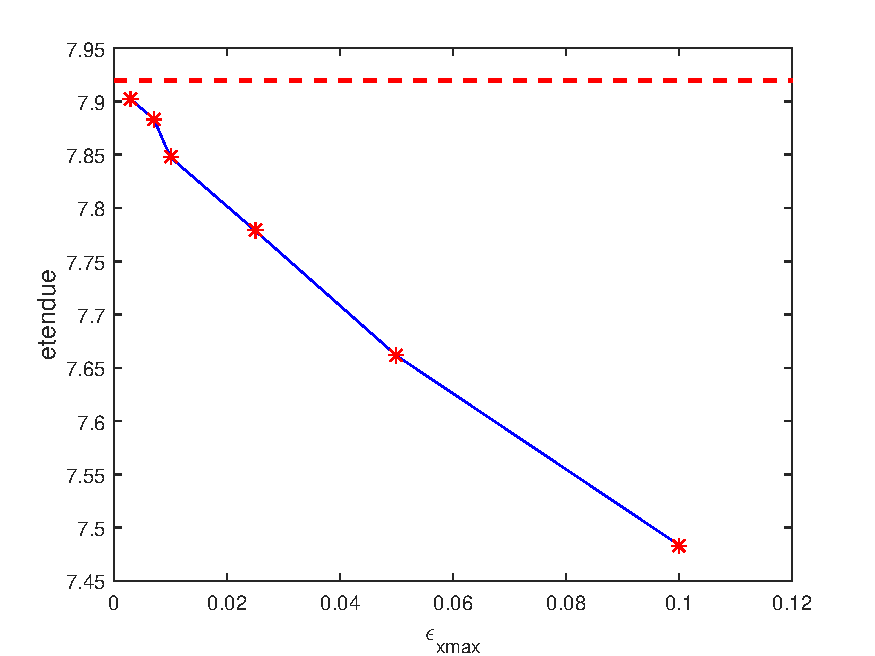
\includegraphics[width=7.7cm]{etendue.pdf}
  \end{center}
  \caption{\footnotesize{The total \'{e}tendue as an area in PS is depicted with the dotted red line. The approximated \'{e}tendue is computed for a range of values of $\epsilon_{x_{max}}$. Decreasing the value of the parameter the $\epsilon_{x_{max}}$, the \'{e}tendue increases and reaches a good approximation of the exact \'{e}tendue for $\epsilon_{x_{max}} = 3\cdot 10^{-3}$.
  }}
  \label{fig:etendueTS}
\end{figure}

 The total \'{e}tendue at the target $E_{\textrm{t}}$ is given by the sum of the \'{e}tendues related to each region $R_{\textrm{t}, \Pi_{j}}$:
 \begin{equation}
 \label{eq:etenduetarget}
 E_{\textrm{t}} = \sum_{j = 1}^p E(R_{\textrm{t}, \Pi_j})\,,
 \end{equation}
 where $E(R_{\textrm{t}, \Pi_j})$ is the contribution to the \'{e}tendue at the target given by the rays inside the region $R_{\textrm{t}, \Pi_j}$. Note that $E_{\textrm{t}}$ is computed by also considering the area of the regions formed by the rays that hit the left and the right detectors (lines $13$ and $14$ in Figure \ref{fig:analyticlens}). $E(R_{\textrm{t}, \Pi_j})$ is defined by:
  \begin{equation}\label{etenduepartial}
 E(R_{\textrm{t}, \Pi_j}) = {\int\!\!\int}_{R_{\textrm{t}, \Pi_j}} \textrm{d}q\textrm{d}\eta \,.
 \end{equation}
 To calculate the previous integral the triangulation refinement method is applied to the regions $R_{\textrm{s}, \Pi_j}$ for a range of values of $\epsilon_{x_{max}}$, with an approximation of the boundaries $\partial{R_{\textrm{s}, \Pi_j}}$ obtained for each of them.
 Therefore, the boundaries $\partial{R_{\textrm{t}, \Pi_j}}$ are also computed and the intersection points $(q_{\Pi_j,i}( \eta))_{i = 1, \cdots, r}$ between $\partial R_{\textrm{t},\Pi_j}$
and the horizontal line $\eta ~=~ const$ are calculated for each $j \in \{1, \cdots, p\}$ , with $\eta~\in~[-1,1]$. Ordering the points $(q_{\Pi_j,i}( \eta))_{i = 1, \cdots, r}$ in ascending order,
 Equation ($\ref{etenduepartial}$) becomes:
\begin{equation}
\label{eq:etenduetarg2}
 E(R_{\textrm{t}, \Pi_j}) =\sum_{i = 1}^{m} \int_{-1}^{1}{(q_{\Pi_j, 2i}( \eta)}-{q_{\Pi_j,2i-1} ( \eta) )} \textrm{d}\eta \,,
\end{equation}
where $m$ is the integer part of $r/2$ and $r$ is the number of the intersection points between $\partial R_{t,\Pi_j}$
and the horizontal lines $\eta ~=~ const$. The integral in Equation (\ref{eq:etenduetarg2}) is calculated by discretizing the interval $[-1, 1]$ into $Nb=100$ sub-intervals of equal width and using the trapezoidal rule.
Figure \ref{fig:etendueTS} shows that decreasing the value of the parameter $\epsilon_{x_{max}}$ increases the values of the \'{e}tendue at the target $E_{\textrm{t}}$, which reaches $7.9$  when $\epsilon_{x_{max}}= 0.3\cdot 10^{-3}$. We decide to stop the phase space refinement procedure when a good approximation of the \'{e}tendue is obtained.
Moreover, a criterion to establish the values of $\epsilon_{x_{min}}$ is provided.
For each value of $\epsilon_{x_{max}}$ the  \'{e}tendue for a range of values of $\epsilon_{x_{min}}$ is computed.
As the computation of the boundaries does not depend on the number of rays inside the regions, the \'{e}tendue remains constant when the value of $\epsilon_{x_{min}}$ changes. We choose $\epsilon_{x_{min}}$ as large as possible avoiding to trace rays that do not significantly contribute to the computation of the photometric variables at the target.
The value of $\epsilon_{x_{min}}$ depends on the distribution of the rays in phase space. For our optical system the parameter $\epsilon_{x_{min}}=1$.
Figure \ref{fig:sourcePS} and \ref{fig:targetPS} show the approximation of the boundaries obtained for a set of $ 6.9\cdot 10^4$ rays. Five different paths are found and rays that follow the same path are depicted with the same color. Figure \ref{fig:sourcePS} shows that, choosing the values of the parameters as explained above, the regions $R_{\textrm{s}, \Pi_j}$ almost completely cover the source phase space. As a consequence, the dark areas in Figure \ref{fig:targetPS} correspond to parts of target phase space that are not reached by any ray that leaves the source and propagates though the meridional plane of the optical system. Note that, using the triangulation procedure explained in the previous section, more rays close to the boundaries are traced.

\begin{figure}[h]
  \begin{center}
  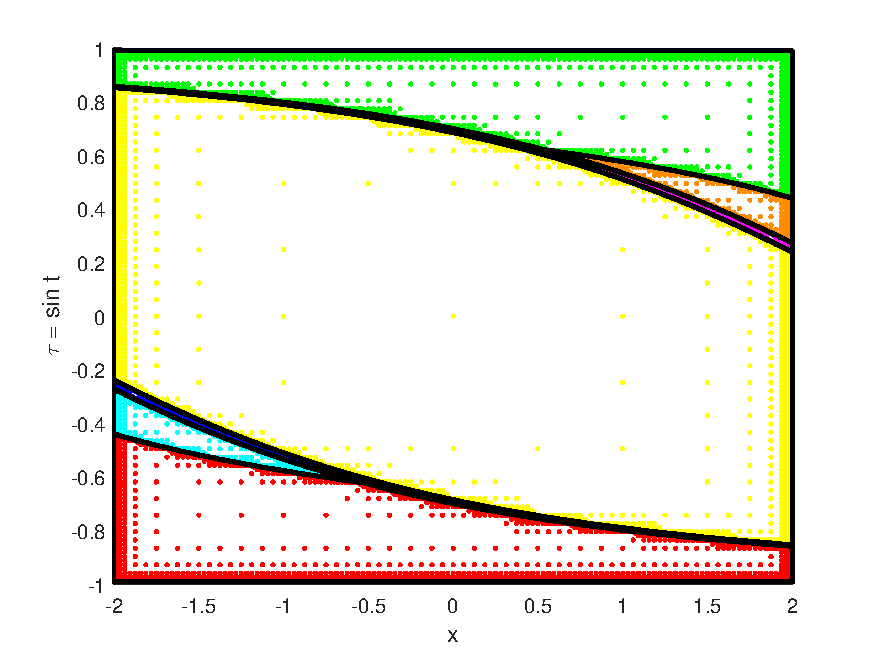
\includegraphics[width=7.7cm]{source1.pdf}
  \end{center}
  \caption{\footnotesize{Distribution of the rays on source phase space. Around $6.9 \cdot 10^4$ rays are traced using the triangulation refinement with parameters:
  $\epsilon_{x_{min}} ~=~ 1 ,$ $ \epsilon_{\tau_{min}} ~=~ 0.5, $ $\epsilon_{x_{max}} ~=~ 3\cdot 10^{-3}, \epsilon_{\tau_{max}} ~=~ 1.5 \cdot 10^{-3}$. Rays that belong to the same region are depicted with the same color. The yellow rays follow the path $\Pi_1 = (1, 2, 7, 12)$;
   the red rays follow the path $\Pi_2 ~= ~(1, 10, 8, 7, 12)$; the green rays follow the path $\Pi_3 = (1, 4, 6, 7, 12)$;
   the blue rays follow the path $\Pi_4= (1, 11, 7, 12)$; the magenta rays follow the path $\Pi_5= (1, 3, 7, 12)$, the cyan rays hit the left detector (line $13$) and follow the path
   $\Pi_6= (1, 10, 7, 8, 13)$ and, the orange rays hit the right detector (line $15$) and follow the path $\Pi_7= (1, 4, 7, 6, 15)$. Each number corresponds to a line of the TIR-collimator as shown in Figure $\ref{fig:analyticlens}$.
  The boundaries are depicted with the black lines.}}
  \label{fig:sourcePS}
\end{figure}


 \begin{figure}[h]
  \begin{center}
  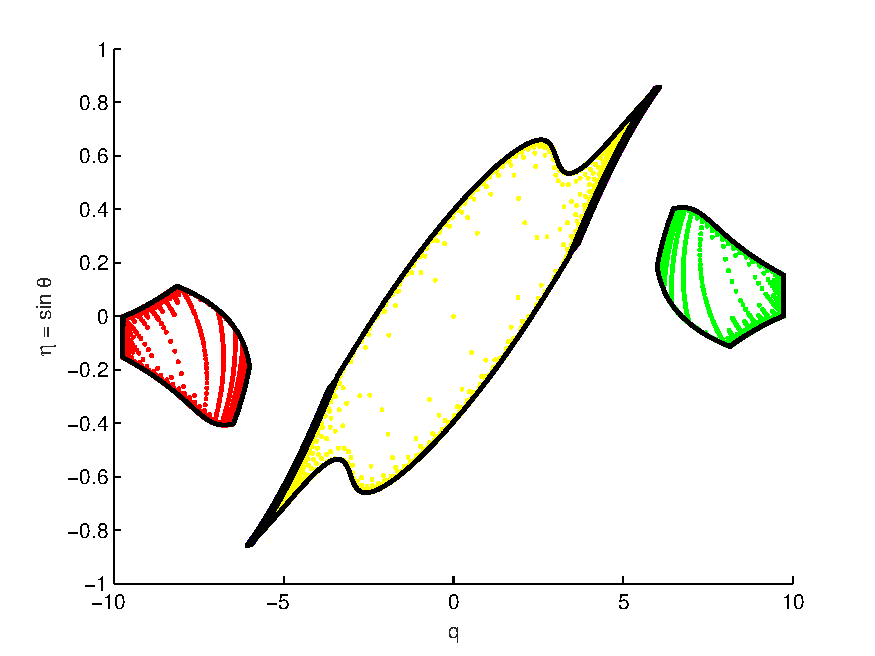
\includegraphics[width=7.7cm]{target.pdf}
  \end{center}
  \caption{\footnotesize{Target phase space representation of a set of $6.9 \cdot 10^4$ rays. Only the rays that hit the target (line $12$) are considered.
  The values of the parameters $\epsilon_{x_{min}}, \epsilon_{x_{max}}, \epsilon_{\tau_{min}}, \epsilon_{\tau_{max}}$ and the choice of the colors for each path are the same as in Figure $\ref{fig:sourcePS}$.
 The boundaries $(\partial R_{\textrm{t}, \Pi_j})_{j = 1, \cdots, p}$ are computed through the triangulation method. The dark areas correspond to areas that are not hit by any meridional plane.}}
  \label{fig:targetPS}
\end{figure}

\indent To conclude, we compute the target intensity which is defined in $\mathcal{P}_{\textrm{t}}$ by Equation (\ref{I(eta)}).
From Equation (\ref{luminance}), we obtain:
\begin{equation}
I_{PS}(\eta) = \sum_{ i, j }\int_{q_{\Pi_j,2i-1}( \eta)}^{q_{\Pi_j, 2i}( \eta)}L_\textrm{t}(q, \eta)\textrm{d}q\,,
\label{eq:Ips}
\end{equation}
where the summation for the indices $i$ is over all $i = 1,2, \cdots, m$, and the summation for the $j$ indices is over all $j$ for which the intersection between $\eta = const$ and $R_{t, \Pi_j}$ is not empty. The intensity is expressed as a function of the angular parameter $\eta~ = ~n_{t}\sin(\theta)$.
In the case of a Lambertian source with $L_{s}(x, \tau) = 1$,
 the following relation for the intensity at the target holds:
\begin{equation}
I_{PS}(\eta) =
\sum_{i,j}(q_{\Pi_j, 2i}(\eta)-q_{\Pi_j,2i-1}(\eta))\,, \label{intensity_eta}
\end{equation}
where the relation  $n_{\textrm{t}}=1$ and conservation of luminance along a ray are exploited, (see \cite{chaves2008introduction}, chapter 16).
We again notice that Equation ($\ref{eq:Ips})$ and (\ref{intensity_eta}) are valid when only two intersection points are found.
If $r>2$ intersection points occur the sum of the distances $(q_{2i}-q_{2i-1})_{i=1, \cdots, m} $ needs to be computed. To calculate the intensity for all the possible directions, a uniform partitioning
$P ~:~ -1\leq \eta_0< \eta_1 \cdots < \eta_{Nb}\leq 1$ of the interval $J = [-1,1]$ is considered, where $Nb= 100$. Eventually, the intensity for each $\eta_h$, with $h = 0,1, \cdots, Nb$, is obtained using relation ($\ref{intensity_eta}$).
  We compare the new method with the already existing MC ray tracing to show its efficiency.\\
 \indent The intensity for MC ray tracing is computed as follows.
 The partitioning $P$ of $J = [-1, 1]$, used for the target phase space, is considered and the number of rays that fall into each bin $([\eta_h, \eta_{h+1}])_{h = 0, \cdots, Nb-1}$ is
 calculated for all $ h \in\{0, \cdots, Nb-1\} $. The intensity in the direction $\eta_k \in [\eta_h, \eta_{h+1}]$ is approximated by:
 \begin{equation}
 \hat{I}_{MC}(\eta_k) = \frac{Nr([\eta_h, \eta_{h+1}])}{Nr([-1, 1])}, \end{equation}
 for every $\Big(\eta_k = \frac{1}{2}(\eta_{h+1}+\eta_h)\Big)_{k = 1,2, \cdots, Nb}$, where we have indicated
 the number of rays that fall into the bin $[\eta_h, \eta_{h+1}]$ with $Nr([\eta_h, \eta_{h+1}])$
 and the total number of rays with $Nr([-1, 1])$. As $\hat{I}_{MC}$  is normalized, a normalization
 of $I_{PS}$ is also required to compare the two intensities.
 This normalization is calculated dividing the intensity by the \'{e}tendue $E_{\mathcal{T}}$ at the target:
 \begin{equation}
 \hat{I}_{PS}(\eta_k) = \frac{1}{E_{\mathcal{T}}} \int_{\eta_h}^{\eta_{h+1}}{I}_{PS}(\eta)\textrm{d}\eta \quad \mbox{for} \quad k = 1,2, \cdots, Nb\,,
 \end{equation}
where ${E_{\mathcal{T}}}$ is obtained by removing the \'{e}tendue corresponding to the regions formed by the rays that hit the left and the right detectors from the total \'{e}tendue $E_{\textrm{t}}$, computed in Equation (\ref{eq:etenduetarget}) and shown in Figure \ref{fig:etendueTS},
Note that the intensities are vectors of length $Nb$, and $\hat{I}_{PS}(\eta_k)_{k = 1,2, \cdots, Nb}$ represent the intensities along the directions $(\eta_k)_{k = 1, \cdots, Nb}$.
The accuracy of the intensity also depends on the number of bins considered in the partitioning $P$.
 Choosing $Nb=100$ results in a smooth profile of the intensity;
 hence, we decide to fix that value of $Nb$.
The photometric variables at the target are now determined for MC and PS method.
The numerical results are shown in the next section.

In this section a comparison between the MC and PS methods is presented.
The MC and PS intensities are calculated several times increasing the number of rays $Nr$ to improve the accuracy.
Both approximate intensities are compared with an intensity taken as a reference.
For some optical systems, there is an explicit solution for the target intensity but this is not the case for the TIR-collimator.
Therefore, the reference intensity $\hat{I}_{\mbox{ref}}$ is obtained considering $1,7 \cdot 10^8$ rays in the MC simulation.
We show how the error,
defined as:
\begin{equation}\label{error}
\mbox{error} = \frac{\sum_{h = 1}^{Nb}| \hat{I}_{PS}(\eta_h) - \hat{I}_{\mbox{ref}}(\eta_h)|}{Nb}\,,
\end{equation}
decreases with the increase in the number of rays.
Table \ref{tab:table} describes how the number of rays traced affects the error estimation and shows the correlation between \'{e}tendue and the number of rays, which is
determined by the values of $\epsilon_{x_{min}}$, $\epsilon_{\tau_{min}}$, $\epsilon_{x_{max}}$ and $\epsilon_{\tau_{max}}$ as explained in Section \ref{sec:method}\ref{subsec:triangulation1}.
 Next, the intensity  $\hat{I}_{MC}$ for the MC method is computed.
Replacing $\hat{I}_{PS}$ with $\hat{I}_{MC}$ in Equation (\ref{error}), the error between the reference intensity and the MC intensity is calculated.
Increasing the number of rays traced in MC ray tracing, the error gradually decreases.
In Table $\ref{tab:table2}$ the numerical results are reported.
\begin{table}[htbp] \label{tab:table}
\centering
\caption{\bf Error values of the PS intensity}
\begin{tabular}{lllll}
 \hline  Number \\ of rays\;   & $\epsilon_{x_{max}} $   \;  & $\epsilon_{\tau_{max}}$\; & \'{e}tendue  & $\mbox{error}$\\
  \hline $1\,403$  & $1.0\cdot 10^{-1}$   & $5.00\cdot 10^{-2}$ & $7.4836$ & $3.57\cdot10^{-4}$ \\
$3\,237$    & $5.0\cdot 10^{-2}$    & $2.50\cdot 10^{-2}$ & $7.6614$ & $2.22\cdot10^{-4}$  \\
$7\,299$   & $2.5 \cdot 10^{-2}$    & $1.25\cdot 10^{-2}$ & $7.7787$ & $1.38\cdot 10^{-4}$ \\
 $15\,919$    & $1.0\cdot 10^{-2}$   & $5.00 \cdot 10^{-3}$ & $7.8475$ & $7.31\cdot 10^{-5}$ \\
 $33\,651$   & $7.0\cdot 10^{-3}$   & $3.50 \cdot 10^{-3}$ & $7.8839$ & $3.80\cdot 10^{-5}$ \\
 $69\,330$  & $3.0\cdot 10^{-3}$    & $1.50 \cdot 10^{-3}$ & $7.9017$ & $2.02\cdot 10^{-5}$ \\
 \hline
 \end{tabular}
 \label{tab:table}
 \end{table}

\begin{table}[htbp]
\centering
\caption{\bf Error values of the MC intensity}
\begin{tabular}{ll} \hline   Number of rays\; & $\mbox{error}_{MC}$\\ \hline $970$  & $2.20\cdot10^{-3}$ \\
$9\,702$  & $6.60\cdot 10^{-4}$  \\ $97\,104$  & $1.74\cdot 10^{-4}$ \\ $971\,436$  & $6.34\cdot 10^{-5}$ \\ $9\,715\,391$  & $2.06\cdot 10^{-5}$ \\
 \hline
 \end{tabular}
 \label{tab:table2}
 \end{table}
\indent The results listed in Table $\ref{tab:table}$ and Table $\ref{tab:table2}$ are shown in Figure $\ref{fig:error}$, where the red line depicts the behavior of the error for the PS
intensity, and the blue line indicates the error for the MC simulation.
\begin{figure}[h!]
  \begin{center}
  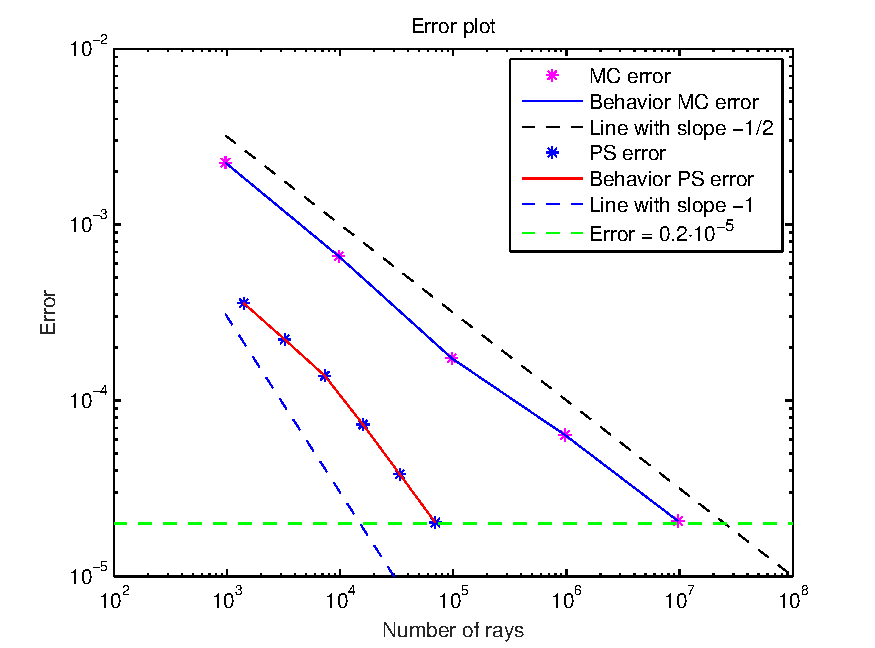
\includegraphics[width=7.7cm]{error.pdf}
  \end{center}
  \caption{\footnotesize{ The red line depicts the error between the intensity on phase space and the reference intensity.
 The blue line shows the error between the Monte Carlo intensity and the reference intensity.
  The dashed black line represents a straight line with the slope equal to $-\frac{1}{2}$.
  The dashed blue line represents a straight line with the slope equal to $-1$.
  The horizontal dotted line shows that an error equal to $2.00 \cdot  10^{-5}$ can be obtained tracing at least $10^2$ times fewer rays in phase space.}}
  \label{fig:error}
\end{figure}
\\
\indent Figure $\ref{fig:error}$ shows that an error equal to $2.00 \cdot  10^{-5}$ is obtained by tracing around $9.7 \cdot 10^{6}$ rays for
MC and only around $6.9 \cdot 10^4$ in PS. The error decreases as $\frac{1}{\sqrt{Nr}}$ for the MC method and as $\frac{1}{Nr}$ for the PS simulation.
  \begin{figure}[h]
    \centering
    \begin{minipage}[]{.40\textwidth}
    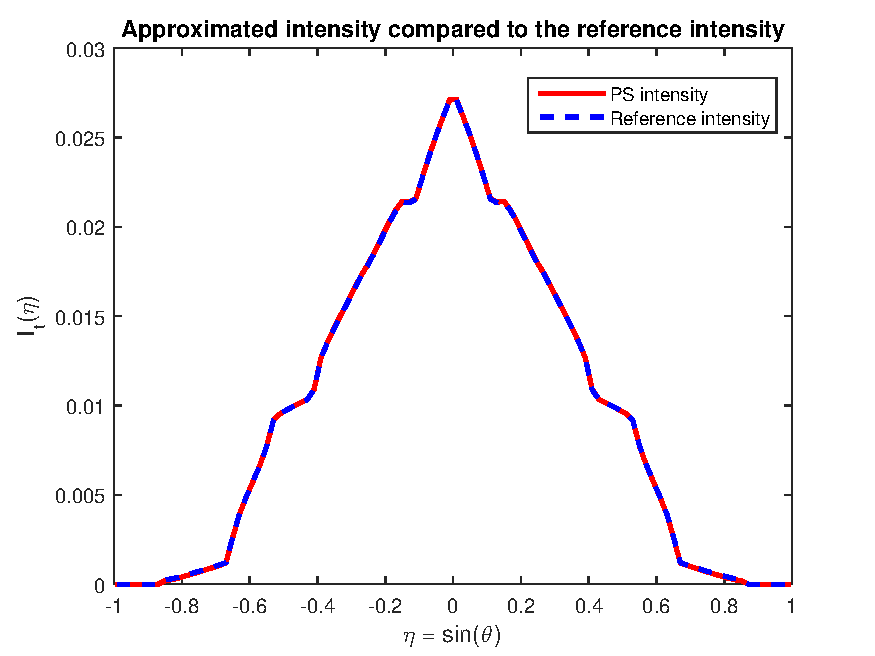
\includegraphics[width=7.7cm]{intensity.pdf}

\caption{\footnotesize{The red line shows the PS intensity at the target of the TIR-collimator. The reference intensity is depicted with the dotted blue line.
The approximate intensity can hardly be distinguished from the exact
intensity. The curves are functions of the angular parameter $\eta = n_{t}\sin(\theta)$. }}
  \label{fig:intensityMCPS}
    \end{minipage} \vspace{2em} \qquad \qquad \qquad
  \end{figure}

\indent The intensity profile $\hat{I}_{PS}(\eta)$ obtained with the phase space method and tracing around $6.9\cdot 10^4$ rays is depicted in Fig. \ref{fig:intensityMCPS} with a red line.
$\hat{I}_{PS}$ is hardly distinguishable from $\hat{I}_{\mbox{ref}}$ (dashed blue line in Figure $\ref{fig:intensityMCPS}$). The intensities are expressed as functions of $\eta$ and thus, the curves in Figure $\ref{fig:intensityMCPS}$ do not depict the spatial intensities.\\
\indent Finally, we claim that PS ray tracing is also more accurate than the ray tracing procedure proposed by Moore (2013), \cite{moore2013methods}.
The novelty of our approach compared to the method used by Moore, is briefly explained below.
First, to compute the output intensity, we employ the phase space of the target. This avoids the use of any interpolation to compute the photometric variables and therefore, more accurate results are obtained.
Second, in \cite{moore2013methods} all rays that leave the source start at the same position and only a sampling angular range is given. In our approach a rectangular source is considered thus, both the angular and spatial coordinates of each ray change. This extra variable can produce very irregular shapes of the regions at target phase space. To overcome this issue, we employ the edge-ray principle and we consider the regions at source phase space where the distribution of the rays is much more regular and the corresponding boundaries are easily computed.
As a consequence, our procedure is suitable to compute the output intensity as function of both the angular or the spatial coordinates.
Third, using the conservation of \'{e}tendue, we provided a criterion to stop the triangulation refinement. In this way we can estimate the number of rays required to obtain the desired accuracy and thus, we avoid tracing more rays than necessary.
\section{Quasi-Monte Carlo method}

\chapter{Ray tracing on phase space} \label{chap:PS}
Ray tracing on phase space is method which employs the phase space (PS) of the source and the target of the optical systems. 
It takes into account of the trajectory that every ray follows during its propagation.
We show through this chapter that this allows to trace only the rays close to the discontinuity of the luminance.
Before explaining the method, we need to introduce the PS concept.
\section{Phase space concept}
The PS of a three-dimensional systems is a four-dimensional space since every ray is described by two position coordinates
and two direction coordinates.
The two position coordinates are given by two of the coordinates of the intersection point of the ray with the surface, while the two direction coordinates are
the momentum coordinates of the vector tangent to the ray projected on the optical surface, see \cite{wolf2004geometric}.
\\ \indent For two-dimensional systems every ray in the PS of a line is given by a point in a two-dimensional space.
The position coordinate in the PS of line $\lineai$ is the \variabile{x}-coordinate of the intersection point between the ray and line $\lineai$.
The direction coordinate is the sine of the angle that the ray forms with respect to the normal of line $\lineai$ multiplied by the index of refraction of the medium in which the ray is located.
We indicate the PS with \set{S}{}{}$=$\set{Q}{}{}$\times$\set{P}{}{},
where \set{Q}{}{} is the set of the position coordinates \variabile{q} and \set{P}{}{} is the set of the direction coordinates $\variabile{p}=\variabile{n}\sin{\myangle}$ with $\myangle$ the angle between the ray and the normal \vect{$\boldsymbol{\nu}$} of the line and \variabile{n} is the index of refraction of the medium in which the line is located.  
The normal \vect{$\boldsymbol{\nu}$} is always directed inside the same medium in which the incident ray travels and, 
the angle $\myangle$ between the ray and \vect{$\boldsymbol{\nu}$} is measured counterclockwise.
In the following, the phase space is considered only for the source $\point{S}$ and the target $\point{T}$ and for no other line of the optical system.
The coordinates of every ray on \set{S}{}{} and \set{T}{}{} are indicated with $(\variabile{p}_1,\variabile{q}_1)$ and $(\variabile{p},\variabile{q})$, respectively. 
\begin{figure}[h]
  \begin{minipage}[h]{0.55\textwidth}
    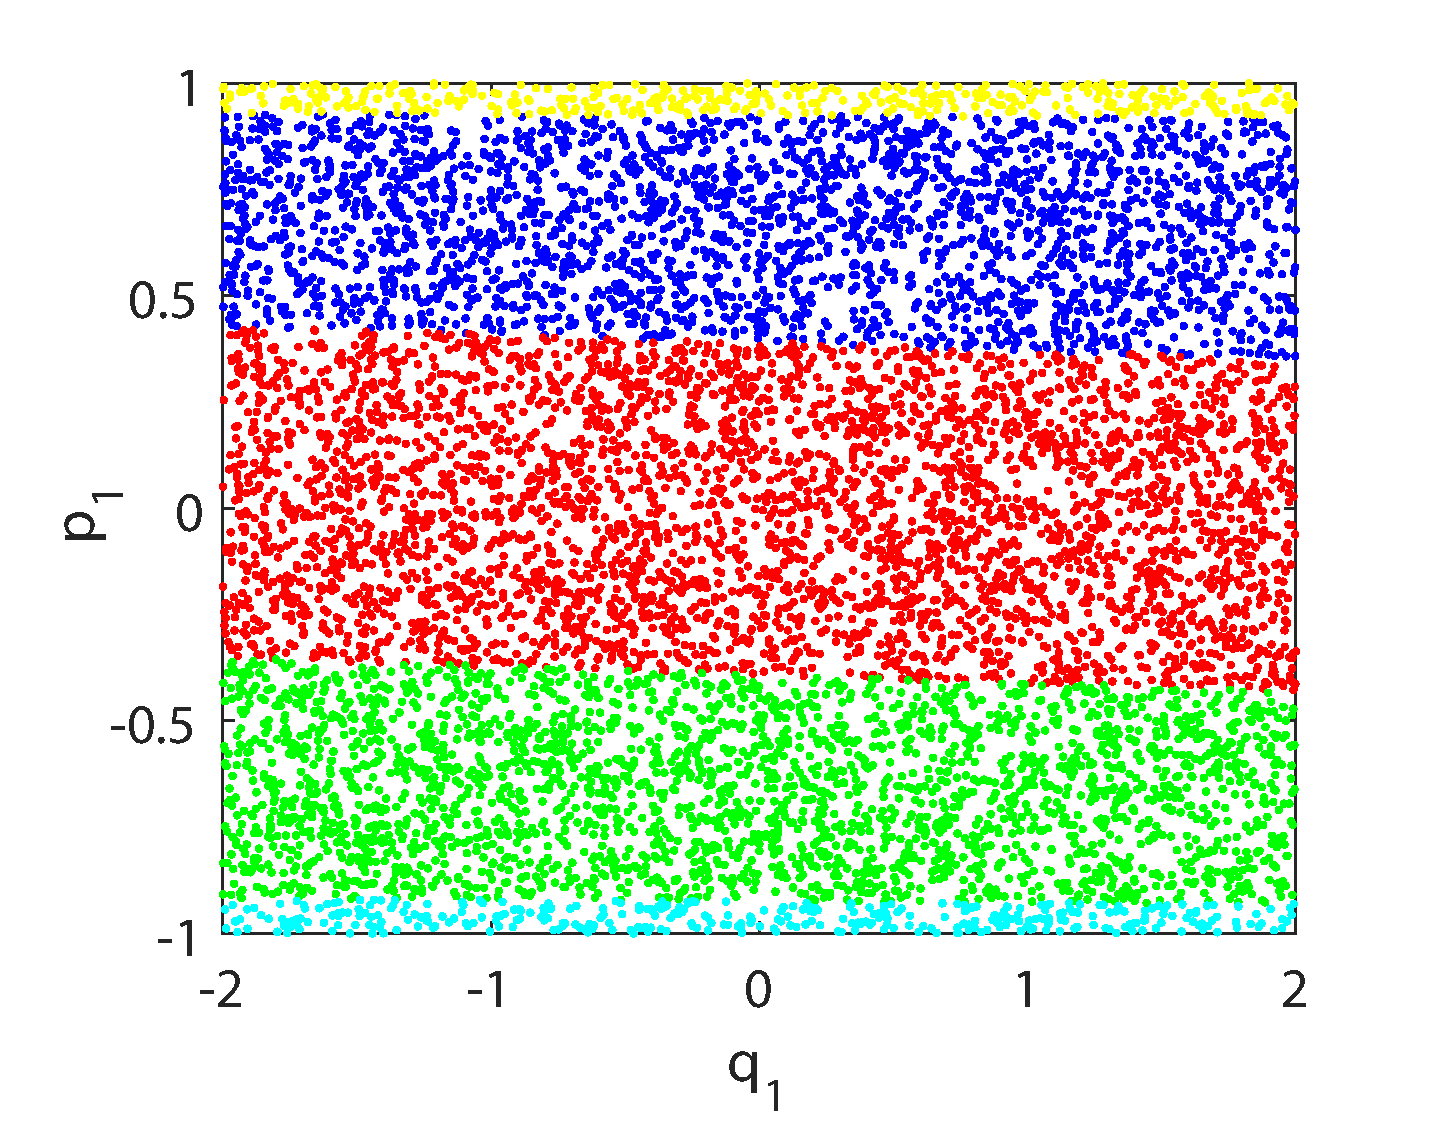
\includegraphics[width=\textwidth]{source_PS_cup.pdf}
    \caption{}
    \label{fig:coefficients}
  \end{minipage} 
  \begin{minipage}[h]{0.55\textwidth}
    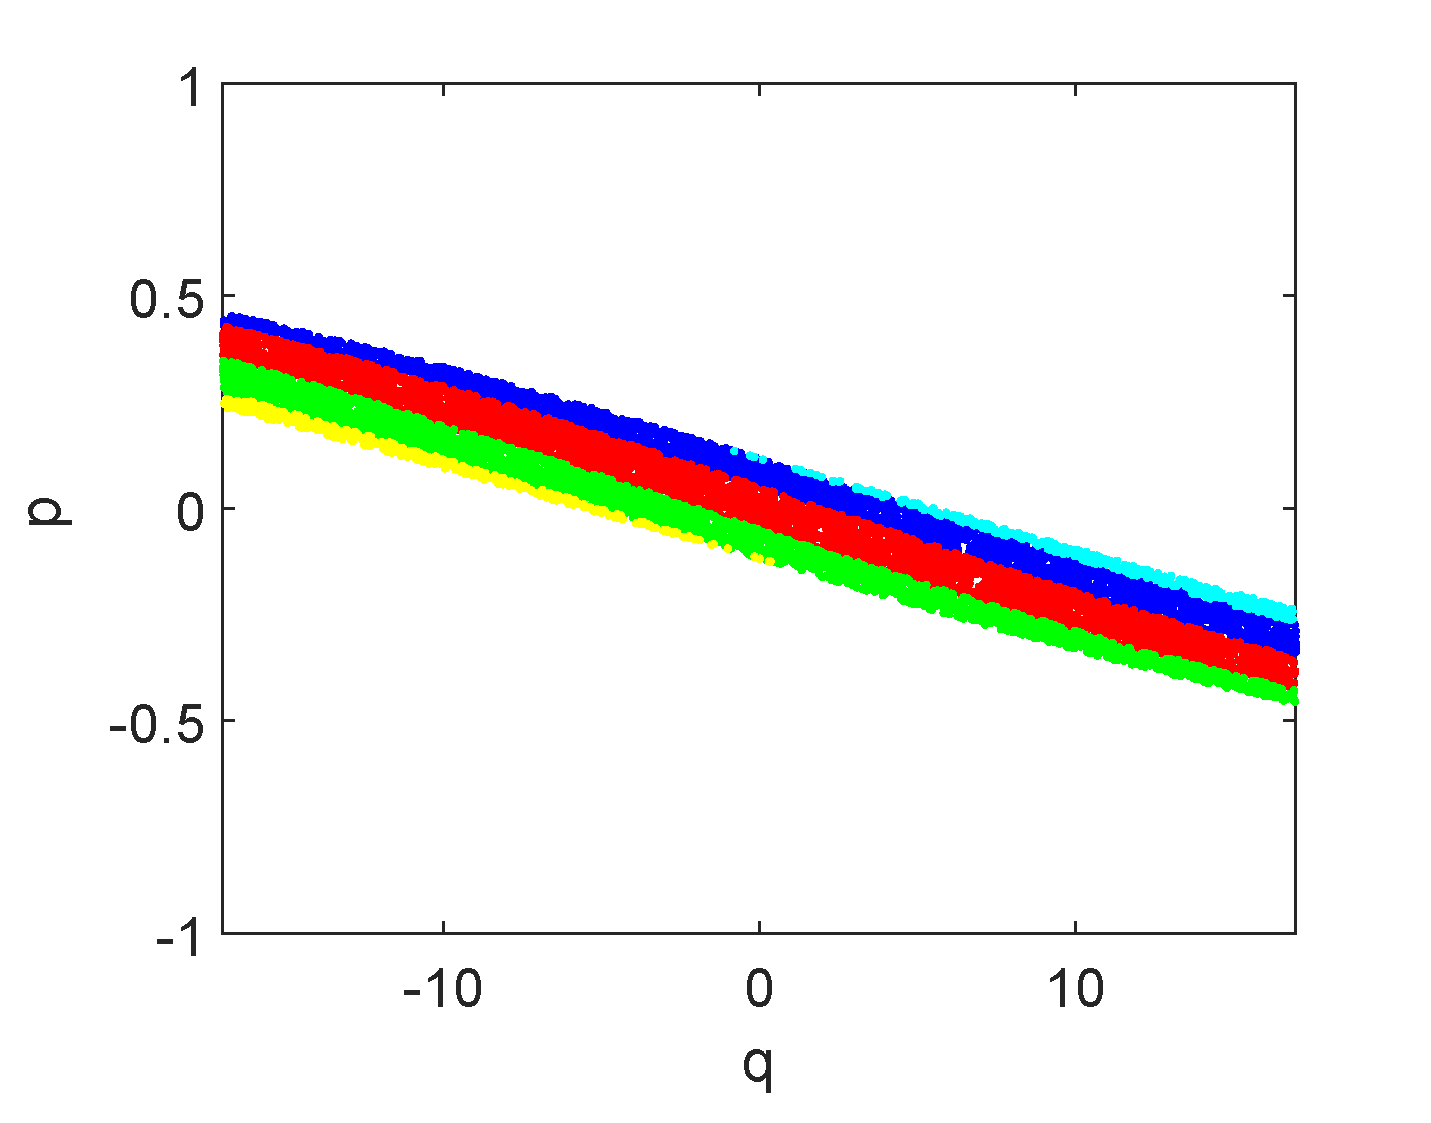
\includegraphics[width=\textwidth]{target_PS_cup.pdf}
    \caption{}
   \label{fig:coefficients2}
 \end{minipage}
\end{figure}
% Show source and target PS
% In fig. \ref{fig:sourcePS} and \ref{fig:targetPS} we show the source and target PS distribution of rays
\\ \indent The source and target phase spaces are partitioned into different regions according to the path $\Pi$ followed by the rays. 
Given a path $\Pi$, the corresponding regions are indicated with \set{R}{$1$}{}$(\Pi)$ and \set{R}{}{}$(\Pi)$ at the source and the target PS, respectively. 
A map $\map{M}{}{}:$\set{S}{}{}$\rightarrow$\set{R}{}{}$(\Pi)\subseteq$\set{T}{}{} which describes how the optical system changes the rays is defined as:
\begin{equation}\label{M}
\map{M}{}{}(\variabile{p}_1,\variabile{q}_1)=(\variabile{p}, \variabile{q}).
\end{equation} 
For very simple systems, as for example the two-faceted cup, it is possible to determine an analytic expression for $\map{M}{}{}$.
This is not the case of most of the optical systems we deal with. 
We can in that case use the edge ray principle, \cite{welford1978problem}.
Ries and Rabl (1994) showed that the boundaries 
$\partial$\set{R}{$1$}{}$(\Pi)$ at the source are mapped into the boundaries $\partial$\set{R}{}{}$(\Pi)$ at the target: all rays that are neighbors at the source PS remain close to each other at the target PS, \cite{Ries:2}. Then, to map one region from the \set{S}{}{} to \set{T}{}{} it is sufficient to map the boundary of this region.
% Say that this is an extended version of the edge-ray principle.
\\ \indent Using the PS concept and the edge-ray principle we develop a new ray-tracing procedure in PS.
\section{Phase space ray tracing}
 
The regions $(R_{\textrm{t}, \Pi_j})_{j =1, \cdots, p}$ can be defined only when some rays are traced.
Given an initial set of rays, the rays closest to the boundaries $(\partial R_{\textrm{t}, \Pi_j})_{j = 1, \cdots, p}$ are selected and more rays in their vicinity are created to get progressively better estimates of the boundaries. A more detailed description is provided below.
A triangulation in $\mathcal{P}_\textrm{s}$ is defined and a ray from every vertex $(x_k, \tau_k)$ of the triangle is traced.
The procedure starts tracing four rays with coordinates $(x_k,\tau_k)_{k=1, \cdots, 4}$ that are located exactly at the corners of $\mathcal{P}_\textrm{s}$ and, for each of them, the paths $(\Pi_{j})_{j = 1, \cdots, 4}$, are stored. Next, for some $j \in\{1, \cdots, 4\}$, the grid is divided into two equal triangles joining two opposite vertices. For each triangle the rays located at its corners are traced. If the paths corresponding to
those rays are different, one or more boundaries
$(\partial R_{\textrm{t}, \Pi_j})_{j =1, \cdots, 4}$ are expected to cross the triangle.
In that case, the middle points $(x_k, \tau_k)_{k = 5, 6, 7}$ of each side of the triangle are added and
three more rays with coordinates $(x_k, \tau_k)_{k = 5, 6,7}$ are traced. Each refinement step leads to four new triangles (see Figure \ref{fig:refinement}).
 \begin{figure}[h]
  \begin{center}
  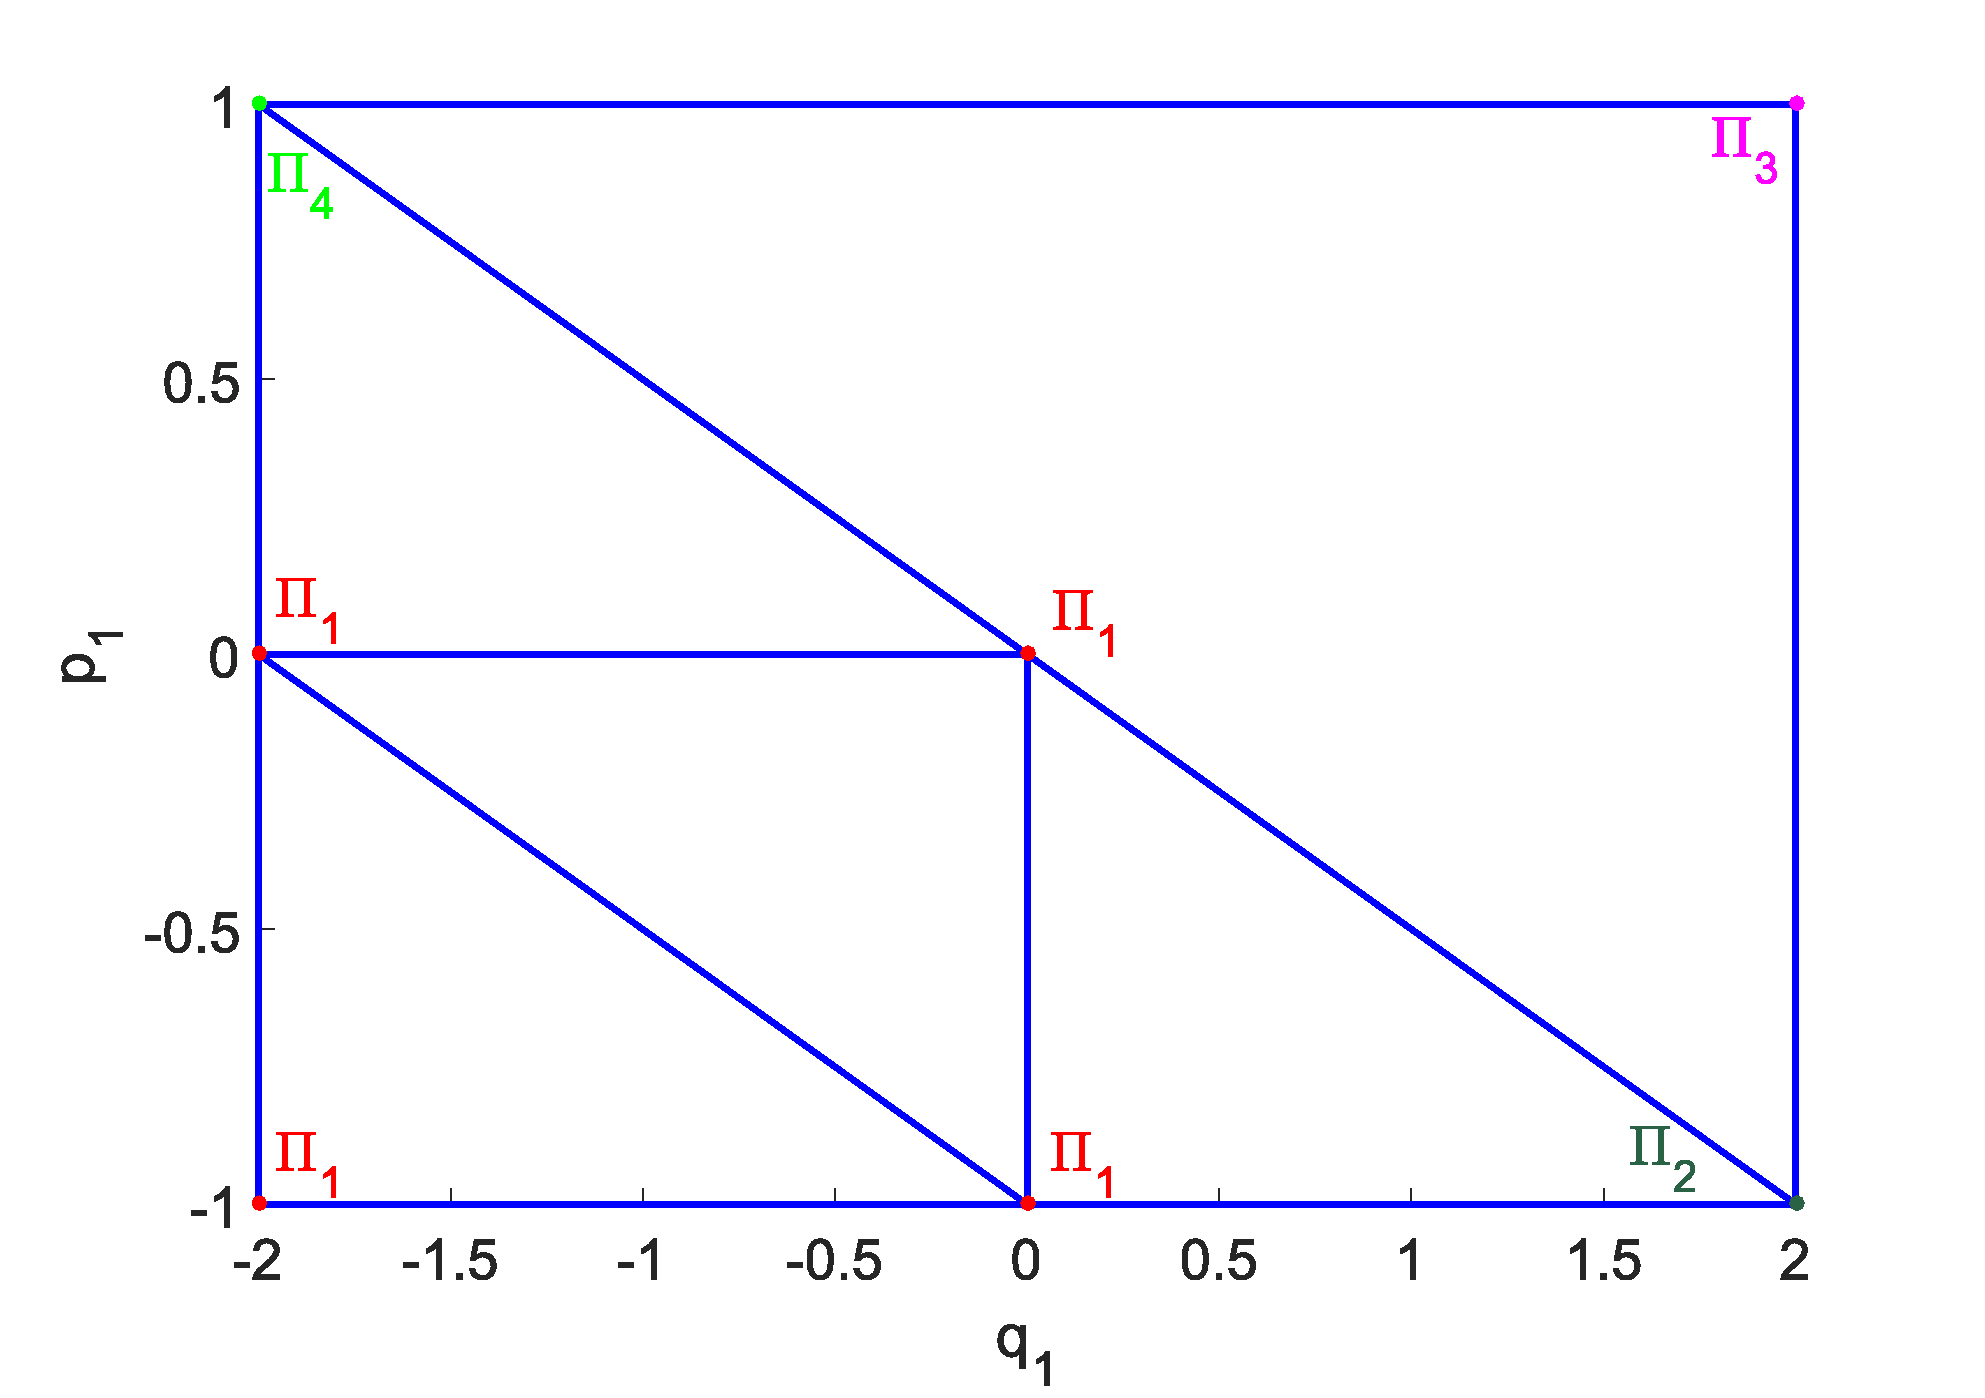
\includegraphics[width=8cm]{region}
  \end{center}
  \caption{Triangulation refinement:
  when the rays related to the vertices of the triangles follow a different path a new refinement step is required.
   Each refinement step leads to four new triangles.
   The parameters values are $\epsilon_{x_{max}}~=~ 2$, $\epsilon_{\tau_{max}}= 1$, $\epsilon_{x_{min}}= 4$ and $\epsilon_{\tau_{min}}=2$.}
  \label{fig:refinement}
\end{figure}
  \\
 \indent
When all the rays in the corners of each triangle have the same path, it is not necessary to refine the triangles anymore.
\noindent Note that it can happen that a region formed by rays that follow a path $\Pi_j$ is located completely inside a triangle whose vertices are related to the same path $\Pi_i$ with $j \neq i$. In that case the algorithm is not able to detect that region, see Figure \ref{fig:region inside}. To avoid this, two parameters $\epsilon_{x_{min}}$ and $\epsilon_{\tau_{min}}$ are defined for the $x$-axis and the $\tau$-axis, respectively. When the length of the sides of the triangle are greater than these parameters, a new triangle is defined even if its vertices correspond to the same path. Furthermore, two other parameters $\epsilon_{x_{max}}$ and $\epsilon_{\tau_{max}}$ are introduced to defined a stopping criterion.
The algorithm stops when the length of the sides of the triangles is smaller than $\epsilon_{x_{max}}$ and $\epsilon_{\tau_{max}}$.
\begin{figure}[h]
  \begin{center}
  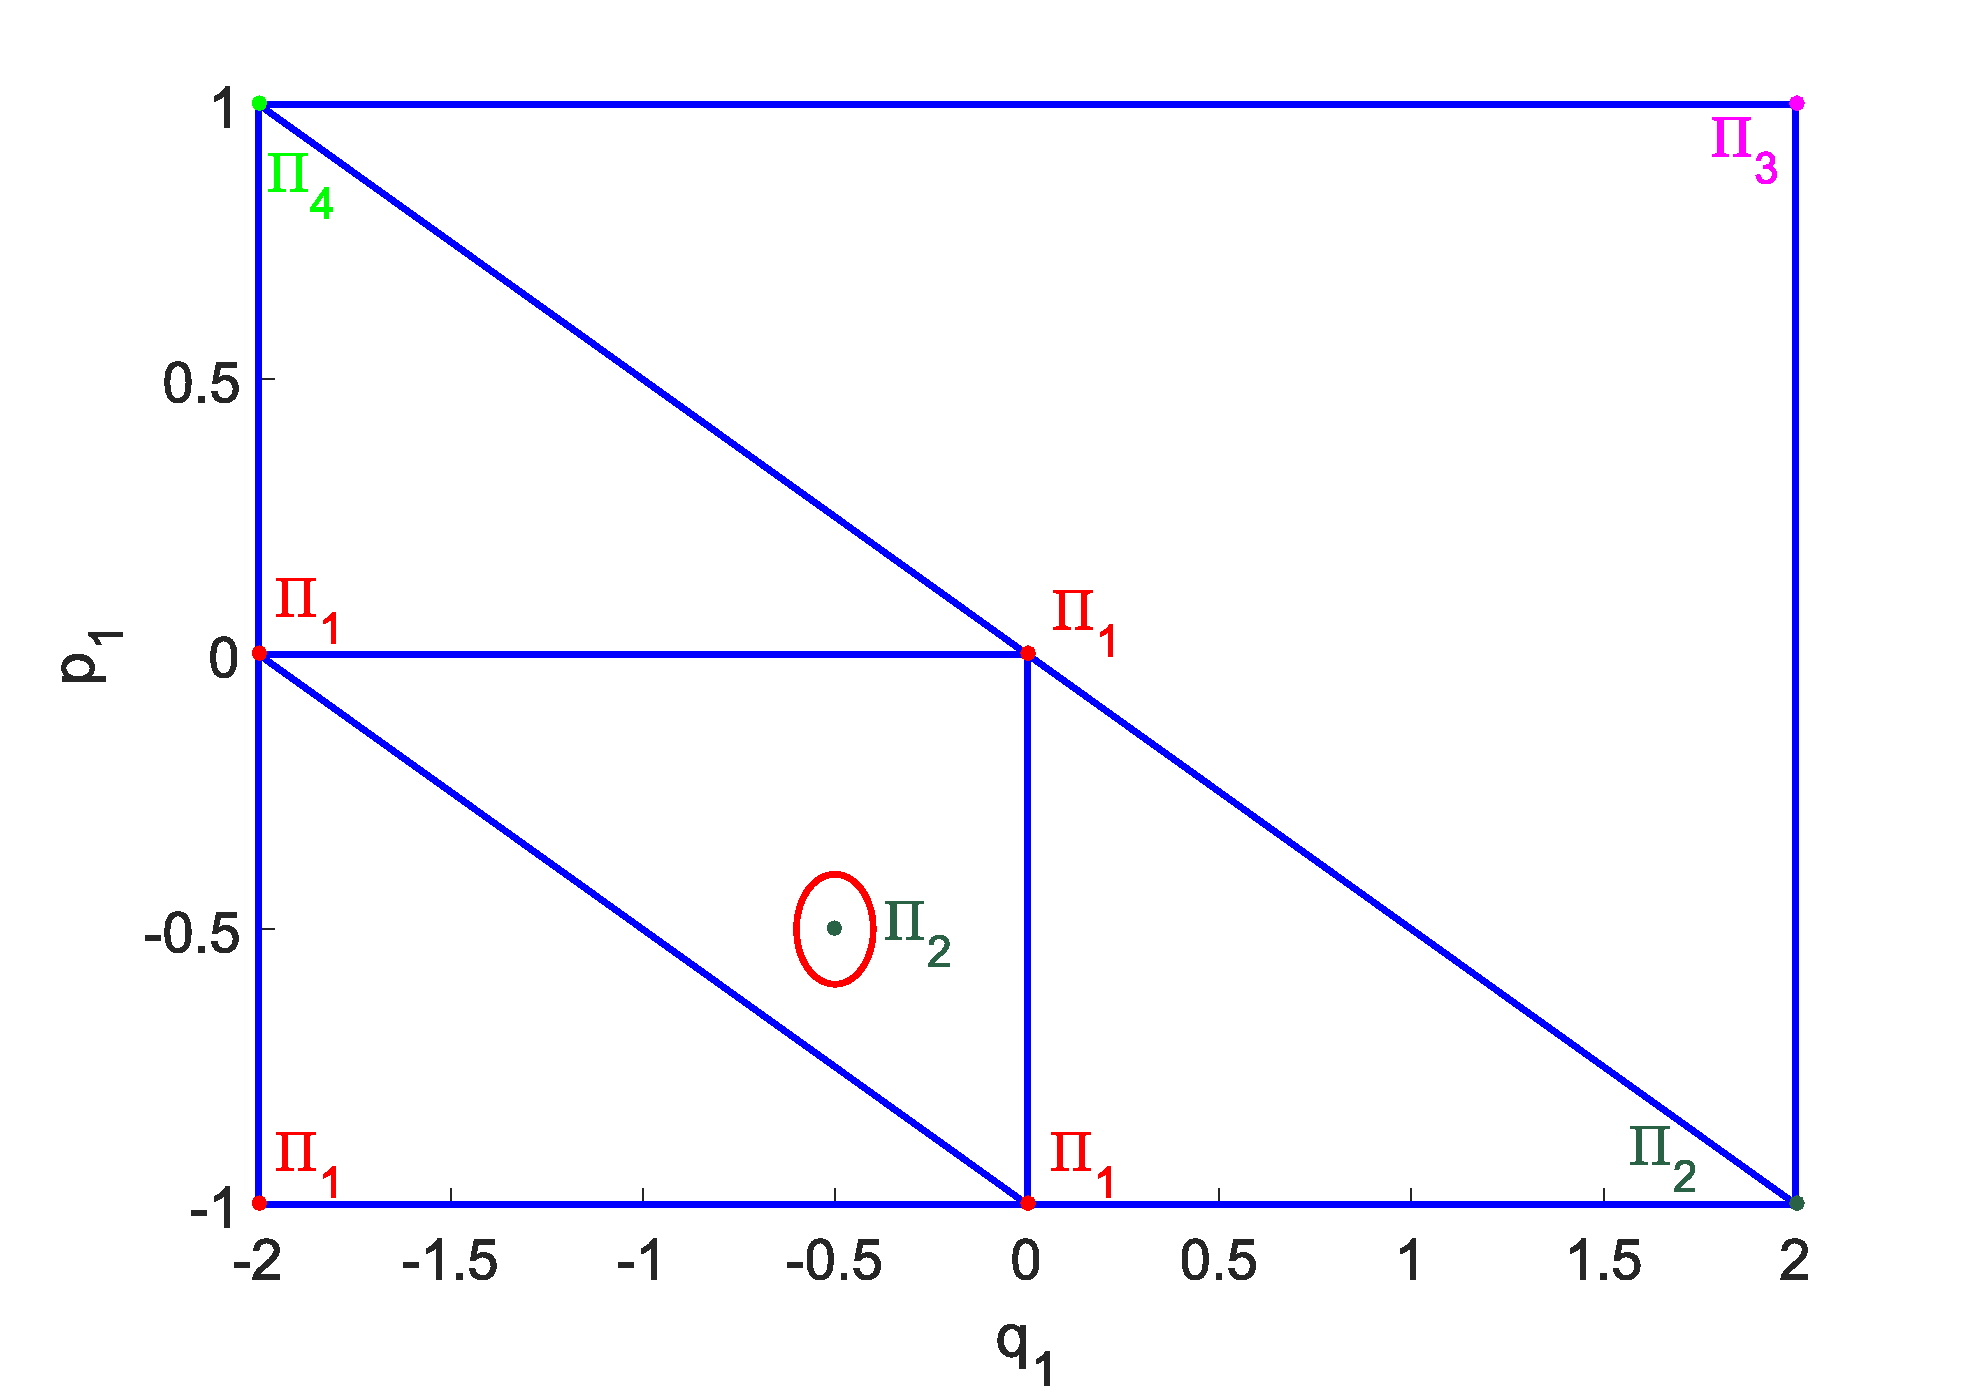
\includegraphics[width=8cm]{region_inside}
  \end{center}
  \caption{The red line encloses a region of rays that follow the path $\Pi_2$ and is completely located inside a triangle.
  The algorithm is not able to detect that region and, a further refinement is required.
    The parameters values are $\epsilon_{x_{max}}~=~ 2$, $\epsilon_{\tau_{max}}= 1$, $\epsilon_{x_{min}}= 4$ and $\epsilon_{\tau_{min}}=2$. }
   \label{fig:region inside}
  \end{figure}
The values of the parameters $\epsilon_{x_{max}}$, $\epsilon_{\tau_{max}}$, $\epsilon_{x_{min}}$ and $\epsilon_{\tau_{min}}$ determine the number of rays traced.
Indeed, on the one hand, $\epsilon_{x_{max}}$ and $\epsilon_{\tau_{max}}$ can be decreased to obtain more rays close to the boundaries;
on the other hand, a large number of rays in the interior of the regions can be traced decreasing the values of $\epsilon_{x_{min}}$ and $\epsilon_{\tau_{min}}$. %
\newline
\indent Using the above procedure, rays increasingly closer to the boundaries are traced.
For our optical system, the width of the $x$-axis in source phase space is two times the width of the $\tau$-axis.
Thus, our choice is $\epsilon_{\tau_{min}}=\frac{1}{2}\epsilon_{x_{min}}$ and $\epsilon_{\tau_{max}} = \frac{1}{2}\epsilon_{x_{max}}$.
Figure \ref{fig:triangulation_refinement} shows an example of a triangulation refinement of the source phase space with $\epsilon_{x_{max}}=0.1$ and $\epsilon_{x_{min}}=1$.
The triangulation refinement provides more triangles close to the boundaries $\partial R_{\textrm{s}, \Pi_j}$ than those inside the regions $R_{\textrm{s}, \Pi_j}$.
\begin{figure}[h]
  \begin{center}
  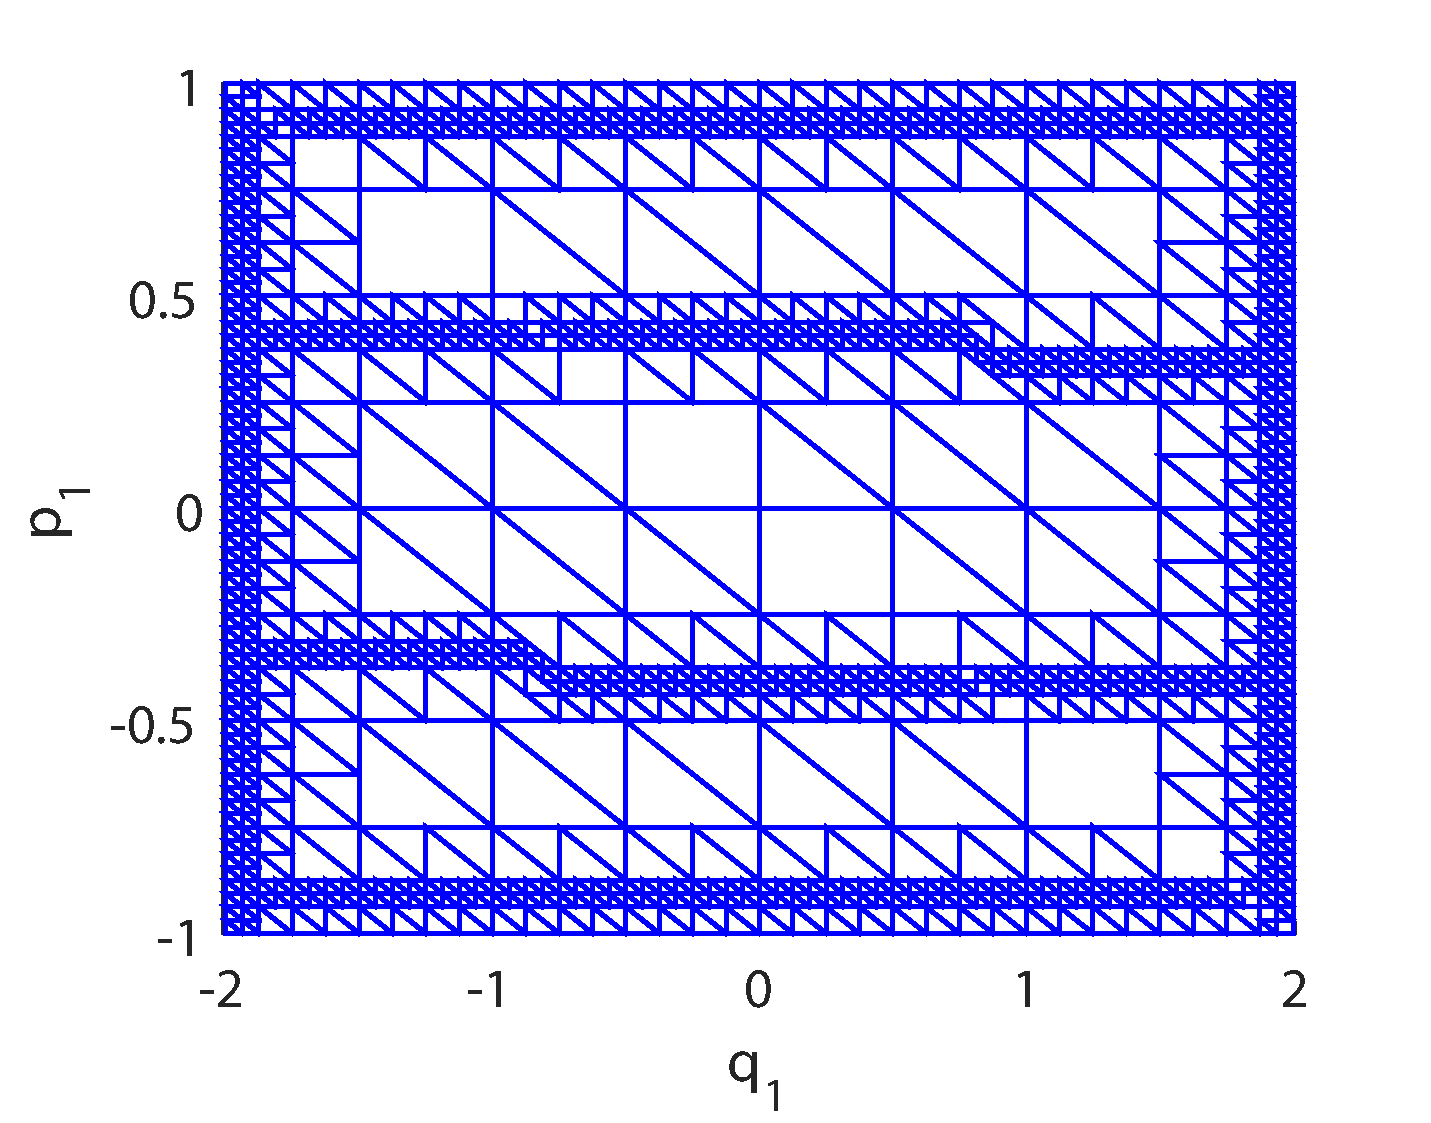
\includegraphics[width=8cm]{triangulation_source}
  \end{center}
  \caption{Triangulation refinement of source phase space:
  near the boundaries more rays are traced.
    The values of the parameters are $\epsilon_{x_{max}}~=~ 0.1$ and $\epsilon_{x_{min}}~=~1$.}
   \label{fig:triangulation_refinement}
  \end{figure}
 \\ \indent The paths $(\Pi_j)_{j = 1, \cdots, p}$ followed by the rays located at the corner of the triangles are computed during the procedure and, the regions
 $R_{\textrm{s}, \Pi_j}$ and $R_{\textrm{t}, \Pi_j}$ are defined for each $\Pi_j$.
Next, a criterion to select the values of the parameters $\epsilon_{x_{min}}$ and $\epsilon_{x_{max}}$ and a method to compute the boundaries $\partial{R_{t, \Pi_j}}$ is provided.
Furthermore, the output photometric variables are computed, the details are explained in the next section.



\section{Comparison between MC, QMC and PS ray tracing}

% Compare all the PS
% Definition of luminance intensity and etendue

\indent A similar method as described in this chapter is presented by Moore, \cite{moore2013methods}. In Moore's method each ray leaves the source at the same position while the angle coordinate changes. The path followed by the rays is taken into account and an interpolation is required to finalize the illumination pattern.
 This interpolation can affect the efficiency of the method. Our method employs the distribution of the rays at the target phase space and avoids using any interpolation. 
Moreover, a criterion to stop the algorithm is provided in such a way that no more rays than necessary are traced. This makes ray tracing in phase space more accurate compared with Moore's procedure.
 Finally, we claim that PS ray tracing is also more accurate than the ray tracing procedure proposed by Moore (2013), \cite{moore2013methods}.
The novelty of our approach compared to the method used by Moore, is briefly explained below.
First, to compute the output intensity, we employ the phase space of the target. This avoids the use of any interpolation to compute the photometric variables and therefore, more accurate results are obtained.
Second, in \cite{moore2013methods} all rays that leave the source start at the same position and only a sampling angular range is given. In our approach a rectangular source is considered thus, both the angular and spatial coordinates of each ray change. This extra variable can produce very irregular shapes of the regions at target phase space. To overcome this issue, we employ the edge-ray principle and we consider the regions at source phase space where the distribution of the rays is much more regular and the corresponding boundaries are easily computed.
As a consequence, our procedure is suitable to compute the output intensity as function of both the angular or the spatial coordinates.


% We need to compute the boundaries, explained in next chapter



\chapter{The $\alpha$-shapes approach to compute the boundaries in target phase space}\label{chap:boundaries_alpha}
In the previous chapter we presented a new ray tracing approach based on PS. We explained that, in order to compute the target photometric variable, it is useful to know the boundaries of the regions with positive luminance in target PS. Ray tracing in PS allows tracing only the rays close to these boundaries. 
\\ \indent To detect the shape formed by those rays, the $\alpha$-shapes approach is employed, \cite{portegies2013fast}. 
Methods based on $\alpha$-shapes are widely used to reconstruct an unknown surface from a set of data points, \cite{guo1997surface}. 
The main disadvantage of such methods is that it can be very hard to chose the suitable value of the parameter $\alpha$ and, in most cases it can be selected only by numerical simulations.\\ \indent
We develop a technique based on $\alpha$-shape that gives a criterion to determine the value of the parameter $\alpha$ for which the better approximation of the boundaries is obtained, \cite{filosa2015new}.\\ \indent This chapter is divided as follows. An overview of the state of art about $\alpha$-shapes methods is provided in Section \ref{sec:alpha-shapes}; the technique used for computing the $\alpha$ value is explained in Section \ref{sec:Tir_alpha}; the results for two different kind of total internal reflection (TIR) collimator are given in the last paragraph of this chapter.
\section{The $\alpha$-shapes approach}\label{sec:alpha-shapes}
Given a finite set $V$ of points, $\alpha$-shapes are geometrical objects that give us an approximation of the shape\footnote{It will become clear through this chapter what we intend with the word \textit{shape}.} formed by the points in $V$.\\ \indent
Before giving a formal definition, we explain an intuitive and nice interpretation of $\alpha$-shapes, \cite{lucieer2004alpha}. 
Let us think to a mass of a stracciatella ice-cream\footnote{Stracciatella ice cream is made with milk-based ice-cream and fine peaces of chocolate, \cite{Wiki3}.}. If we desire to know the shape formed by the chocolate pieces we can start eating the ice cream using a spoon with a spherical shape and trying to do not remove any piece of chocolate. 
We will obtain a shape formed by arcs and points (see Figure \ref{fig:shape2d} for the two-dimensional case).
\begin{figure}[t]\label{fig:shape2d}
\begin{center}
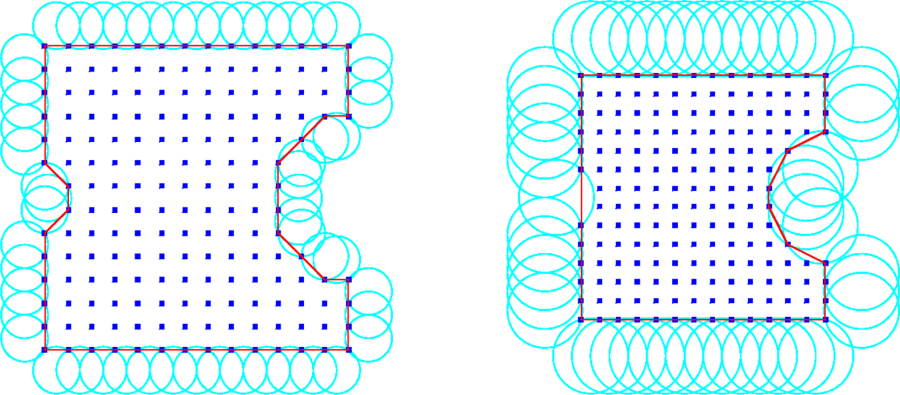
\includegraphics[width=\textwidth]{alpha_shapes2D}
\label{fig:shape}
\caption{Construction of $\alpha$-shape given a set of points (blue dots) in $\mathbb{R}^2$. The boundary of the shape formed by the points cloud (red line) is detected for $\alpha = 1$ (left) and for $\alpha=2$ (right) \cite{sabel2017application}.}
\label{fig:shape2d}
\end{center}
\end{figure}
Straightening the arcs to line segments we obtain broken lines which constitute the boundaries of the so-called $\alpha$-shape formed by the points of the points set $V$. 
A very small spoon will allow us to eat the entire ice cream without eating any piece of chocolate, while with a huge spoon we will not be able to eat any part of the ice cream because at least one chocolate peace will be removed from the ice-cream mass. In this example, the chocolates peaces are the points of $V$ and, the parameter $\alpha$ determines the radius of the carving spoon (the spherical spoon in two-dimension is simply a circle).\\ \indent 
The formal definition of $\alpha$-shape was first given by Edelsbrunner, Kirkpatrick and Seidel in 1983, \cite{edelsbrunner1983shape}. They describe $\alpha$-shape has a generalization of the convex hull of a finite set of point in the plane. Let $\alpha$ be a not negative number $0\leq\alpha<\infty$. 
If $\alpha$ is equal to $0$ the shape degenerates to the point set $V$. On the other hand, when $\alpha\rightarrow\infty$ the $\alpha$-shape is simply the convex hull of $V$. If $0<\alpha<\infty$ the $\alpha$-shape is a polytope of $V$ \cite{edelsbrunner1994three}. The construction of $\alpha$-shape is closely related to Delaunay triangulation of $V$\cite{mucke1993shapes}. Therefore, a formal definition of triangulation and Delanauy triangulation is now required. \\ \indent
Given a set $V$ of not all aligned points, let us consider the set $E$ of all the straight line segments whose endpoints are in $V$. 
A triangulation $T$ of $V$ is the maximum subset of $E$ such that all the line segments of $T$ intersect only at their endpoints \cite{lloyd1977triangulations}. \\ \indent 
The Delaunay triangulation $T^{\prime}$ of the points set $V$ has the property that the circle circumscribed by any triangle of $T$ does not contain any point of $V$. This is called the Delaunay property. A very common used algorithm to construct such triangulation is explained in the following. 
$T^\prime$ is constructed by modifying a general triangulation $T$ such that every point satisfies the Delaunay property. 
Therefore, every triangle (or tetrahedron in three dimensions) that does not satisfy such property is flipped such that the new edge is part of the triangulation (see Figure \ref{fig:Delaunay}). 
Given, for example, an arbitrary triangulation $T$ in two-dimension, for each edge $\overline{\textrm{ab}}$ in $T$ which is not on the boundary of the convex hull the two triangles 
$\Delta_{\textrm{abc}}$ and $\Delta_{\textrm{abd}}$ with the common edge $\overline{\textrm{ab}}$ are found. Then, if either the circumcircle of triangle $\Delta_{\textrm{abc}}$ contains point $d$ or the circumcircle of triangle $\Delta_{\textrm{abd}}$ contains point $c$ the edge $\overline{ab}$ cannot be included in the Delaunay triangulation and, therefore, it is flipped such that the other two possible triangles $\Delta_{\textrm{acd}}$ and $\Delta_{\textrm{bcd}}$ are found. The new edge $\overline{\textrm{cd}}$ locally satisfies the Delaunay property and the triangles $\Delta_{\textrm{acd}}$ and  $\Delta_{\textrm{bcd}}$ are added to the Delaunay triangulation $T^\prime$, see Figure \ref{fig:Delaunay}.  
\begin{figure}[h]\label{fig:Delaunay}
\begin{subfigure}[t]{0.48\textwidth}
\centering
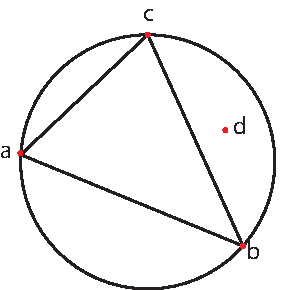
\includegraphics[]{triangle_alpha_shapes}
\label{fig:shape}
\caption{The point $d$ is inside the circle circumscribed by the triangle $\Delta_{\textrm{abc}}$, therefore the edge $\overline{\textrm{ab}}$ cannot be included in the Delaunay triangulation.}
\end{subfigure}
\begin{subfigure}[t]{0.48\textwidth}
\centering
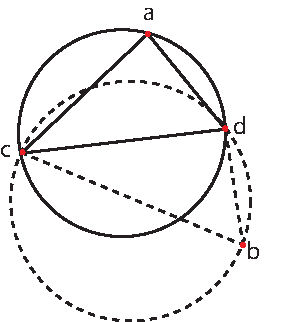
\includegraphics[]{triangle_alpha_shapes_flipped}
\caption{The flipped triangle $\Delta_{\textrm{acd}}$ satisfies the Delaunay property, thus it is included in the Delaunay triangulation.}
\end{subfigure}
\caption{Construction of the Delaunay triangulation in 2D.}
\label{fig:Delaunay}
\end{figure}
\\ \indent Several others algorithm have been developed to construct a Delaunay triangulation, see for example \cite{lee1980two, renka1997algorithm}.
 Given points set $V$ and a triangulation $T$, it can be proved that the corresponding Delaunay triangulation $T^\prime$ is unique. Moreover, it has the property to have the largest minimum angle among all possible triangulation of a point set $V$ \cite{press2007numerical}, and it can be seen as the dual of Voronoi diagram which is defined in the following \cite{fortune1992voronoi}.\\\indent 
Let us consider a finite set of point $V = \{v_1, \cdots, v_N\}\subset \mathbb{R}^2$. For \textit{almost}\footnote{It is needed to specify the word \textit{almost} because some points can have the same distance with two or more points of $V$.} every point $x\in \mathbb{R}^2$, there is a point which is the closest point to $x$. The Voronoi cell of a point $v_\variabile{i}\in V$ contains all points in $\mathbb{R}^2$ which are closer to $v_{\variabile{i}}$, see Figure \ref{fig:Voronoi}. 
The Voronoi diagram of $V\subset \mathbb{R}^2$ is defined as the set of all Voronoi cells, \cite{cazals2005conformal}.  For the definition of Voronoi diagram in higher dimensions see \cite{brown1979voronoi}.
\begin{figure}[h]
\centering
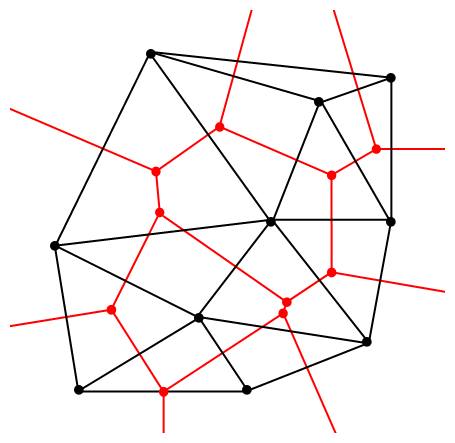
\includegraphics[width = 6cm]{Delaunay_Voronoi}
\caption{Relationship between the Delaunay triangulation (in black) and the Voronoi Diagram (in red), \cite{Wiki4}}
\label{fig:Voronoi}
\end{figure}
%A formal definition of the Voronoi diagram is given in the following.
%\begin{defn}
%Let $X$ be a metric space with a distance $\textrm{d}$ and $V=\{v_1,\cdots,v_N\}$ a set of point in $X$. The Voronoi cell $V_\variabile{i}$ associated with the point $v_\variabile{i}$ with $v_{\variabile{i}}\in\{1,\cdots,N\}$ is defined as:
%\begin{equation}
%V_\variabile{i}=\{x\in X\; | \;\textrm{d}(x,v_\variabile{i})\leq \textrm{d}(x,v_\variabile{j}) \quad \forall \variabile{j}\neq \variabile{i} \}\,,
%\end{equation}
%The Voronoi diagram is defined as the union $U = \bigcup_{\variabile{i}=1}^N V_\variabile{i}$ where $V_{\variabile{i}}\cap V_{\variabile{j}}= \emptyset$ for $\variabile{i}\neq\variabile{j}$.
%\end{defn}
%Figure \ref{fig:Voronoi}
%\begin{figure}[h]\label{fig:Voronoi}
%\begin{center}
%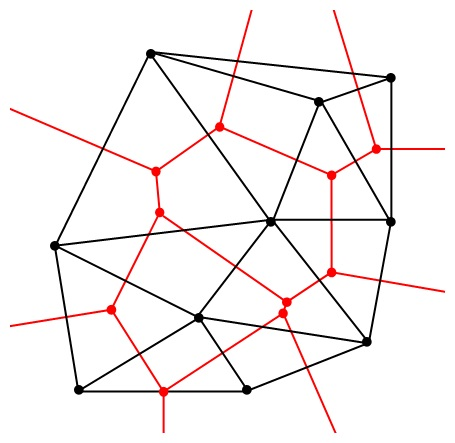
\includegraphics[width=7cm]{Delaunay_Voronoi.jpg}
%\caption{The Delaunay triangulation in black is the dual of the Voronoi diagram in red, \cite{Wiki4}.}
%\label{fig:Voronoi}
%\end{center}
%\end{figure}
Delaunay triangulation triangulates the convex hull of $V$ and, therefore it does not constitutes a suitable method for reconstructing the surface formed by a point cloud. 
\\ \indent Therefore, $\alpha$-shapes methods were developed for surface reconstruction, \cite{edelsbrunner2010alpha, guo1997surface}. Starting from the Delaunay triangulation $T^\prime$ of a point set $V$, the corresponding $\alpha$-shape of $V$ is formed by the only triangles of $T^\prime$ that satisfy the so-called "$\alpha$-test" which is briefly explained in the following.
For each triangle we calculate the radius of the circumcircle. If the radius is larger that $\alpha$ the triangle is removed from the shape. The rule of the parameter $\alpha$ is highly significant in $\alpha$-shapes procedures and, it has to be selected such that the better approximation of the shape formed by the points of $V$ is obtained. 
Therefore, $\alpha$ is closely related to the radius of the circumcircles. A possible strategy is to find the radius of the greater empty circumcircle. Thus $\alpha$ is related to the density $\delta$ of the point sets $V$. It can be chosen, for instance, inversely proportional to $\delta$:
\begin{equation}
\alpha=C\frac{1}{\delta}\;,
\end{equation}
with $C$ a constant and $\delta$:
\begin{equation}
\delta=\frac{N}{\mbox{surface area}}\; ,
\end{equation}
where $N$ is the number of points in $V$ and the surface area is the area inside the boundaries of the region formed by the points cloud. 
For a fixed point set, $\delta$ is given and the value of $C$ needs to be determined by numerical simulations.\\ \indent 
To summarize, $\alpha$-shape procedure can be outlined as follows:
\begin{enumerate}
\item Construct a Delaunay triangulation\footnote{In the simulations we present in this chapter the Matlab function \textit{Delaunay} is used.} $T^\prime$ of the point cloud $V$;
\item For every triangles $T^\prime(i)\in T^\prime$ calculates the radius $r(i)$ of the circle circumscribed by its vertices;
\item If $r(i)\leq\alpha$ keep the triangle $T^\prime(i)$ in the triangulation;
\item If $r(i)>\alpha$ remove the triangle from the triangulation;
\item For every triangle return the edges (facets in $3$D) referred to only one triangle (tetrahedron in $3$D), the so-called \textit{free boundary} edges\footnote{In the simulations we present in this chapter the Matlab function \textit{freeBoundary} is used.}.
\end{enumerate}
%% Insert algorithm
%\begin{algorithm}[h]
%\caption{$\alpha$-shape reconstruction}\label{alg:alphashapes}
%\begin{algorithmic}[1]
%\Procedure{$\alpha$-shape}{$V$, $\alpha$}
%\State Construct a Delaunay triangulation of the point cloud $V$
%\State$T^\prime\gets$ all triangles of the Delaunay triangulation
%\State For every 
%\State Calculates the radius of the circle circumscribed by the vertices of every triangle
%\State $r(i) \gets$
%\State For {every triangle in $T^\prime$}
%\State $(\variabile{q}_1^4, \variabile{p}_1^4) \gets \mbox{left and upper corner of source PS: (-\variabile{a}, 1)} $
%\For{$ \variabile{k}= 1 \to 4 $}
%\State Trace the ray with initial coordinates $(\variabile{q}_1^\variabile{k}, \variabile{p}_1^{\variabile{k}})$ in \set{S}{}{};
%\State Calculate the corresponding path $\Pi^{\variabile{k}}$;
%\State $\mbox{Ray}.\variabile{q}\gets [\mbox{Ray}.\variabile{q}, \variabile{q}_1^\variabile{k}]$;
%\State $\mbox{Ray}.\variabile{p}\gets [\mbox{Ray}.\variabile{p}, \variabile{p}_1^\variabile{k}]$;
%\State Store the corresponding path $\Pi^{\variabile{k}}$.
%\State $\mbox{Ray}.\Pi\gets [\mbox{Ray}.\Pi, \Pi^{\variabile{k}}]$;
%\EndFor
%\State VL $\gets [1, 2, 4]$ \Comment{VL = vertices of the left triangle}
%\State VR $\gets [2,3, 4]$   \Comment{VR = vertices of the right triangle}
%\State \Call{Left Triangle}{VL, Ray, $\varepsilon_{\variabile{q}_1}^{\textrm{min}}, \varepsilon_{\variabile{q}_1}^{\textrm{max}}, \varepsilon_{\variabile{p}_1}^{\textrm{min}}, \varepsilon_{\variabile{p}_1}^{\textrm{max}}$}\Comment{Refine the left triangle} 
%\State \Call{Right Triangle}{VR, Ray, $\varepsilon_{\variabile{q}_1}^{\textrm{min}}, \varepsilon_{\variabile{q}_1}^{\textrm{max}}, \varepsilon_{\variabile{p}_1}^{\textrm{min}}, \varepsilon_{\variabile{p}_1}^{\textrm{max}}$} \Comment{Refine the right triangle} \\
%\Return ;
%\EndProcedure
%\end{algorithmic}
%\end{algorithm}
%\\
%Let us define a Voronoi diagram in a metric space.
%The simplest case that we can have is the two-dimensional case that is the case where $X=\mathbb{R}^2$.
%The tuple $\mathcal{S}=\{1,\cdots,n\}\subset \mathbb{R}^2$ is now a set of points. The Voronoi diagram of $\mathcal{S}$ is a subsection of $\mathbb{R}^2$ such that every other region around a point $p\in \mathcal{S}$ contains all points that are closer to $p$ than to every point in $\mathcal{S}$. A triangulation of the point set $\mathcal{S}$ is a set of edges $\mathcal{E}$ whose extremes are points of $\mathcal{S}$ such that the faces of each triangle are bounded by three edges and any edge that is not in $\mathcal{E}$ intersects one of the existing edges. The Delaunay triangulation is the dual graph of the Voronoi diagram: it consists of vertices (the points in $\mathcal{S}$) and it has an edge between two vertices if the two corresponding faces share an edge. \\
\indent Although $\alpha$-shapes are a powerful tool for surfaces reconstruction, there exist surfaces that are not described well by classical $ \alpha $-shapes. Indeed for some surfaces there is no value of $\alpha$ that includes all desired triangles and deletes all undesired triangles. If the parameter $\alpha$ is determined according to the density of the point cloud, it can be difficult to obtain a good approximation of a shape formed by a non-uniform points set. Furthermore, the $\alpha$-shape method does not work well when the shape we need to approximate has a sharp turn or a joint. 
%In this case $\alpha$-shapes often give a "webbed-foot" appearance at such joints since they improperly connect the adjacent surfaces. 
To overcome these issues, Teichmann and Capps presented alternatives approaches to establish the value of $\alpha$, \cite{teichmann1998surface}. Their anisotropic density-scaled $\alpha$-shapes method constitutes an improvement of  classical $\alpha$-shapes.
\\ \indent There are several ways to determine the value of $\alpha$ \cite{mandal1997selection}; in the next section we provide a technique that exploits the conservation of \'{e}tendue in PS. 
%The first step of this method is to make a triangulation of the point cloud.
%Then the key idea is to compute somehow the point-density of each point and use this to get an approximation of the point density of a triangle. In this way one can reduce the $\alpha$-value in areas where the triangle's point density (see equation \ref{delta_t} for the definition) is higher than average in such a way that is possible to obtain a finer level of detail for areas that have an higher density.
%More precisely, each point $ \textbf{p}\in \mathcal{S} $ has a local point density defined as
%\begin{equation}
%\delta (\textbf{p})= \sum_{\textbf{q}\in \mathcal{S}}\Big( 1-\frac{\textrm{d}(q,p)}{\lambda}\Big) \qquad \forall \textbf{q} \mbox{\;\;such that\;\;} \textrm{d}(\textbf{p},\textbf{q})<\lambda\,,
%\end{equation}
%where $ \lambda $ is the constant radius of the local neighborhood and $\textrm{d}(\textbf{x},\textbf{y})$ is the Euclidean distance.
%When local density is larger than the average, that is when
%\begin{equation}
%\delta (\textbf{p}) >\frac{1}{| \mathcal{S} |}\sum_{\textbf{q}\in \mathcal{S}}\delta (\textbf{q})
%\end{equation}
%we know some properties about the region surrounding $\textbf{p}$.
%For instance, if the point set is uniformly distributed then it is possible to find areas with a high-density in the case where there are two closely separated surfaces.  In point sets of non-uniform distribution, high densities are found when the surface presents a joint discontinuity. The algorithm developed by Teichmann and Capps is structured as follow.
%After computing density information for each point they make a triangulation of the point set. Then they calculate the average density  $\delta(t)$ for each triangle $\Delta_{abc}$ defined as:
%\begin{equation}
%\delta(t)=\frac{\delta(a)+\delta(b)+\delta(c)}{3 \mu}\,,
%\label{delta_t}
%\end{equation}
%where $\mu$ is the global average density of the entire point set $\mathcal{S}$.
%If $\delta(t)$ is greater than $1$ the density of the point cloud is higher. Hence is necessary to define another value of $\alpha$:
%\begin{equation}
%\alpha^{\;\prime} = \frac{\alpha}{\delta(t)^\sigma}
%\end{equation} where $\sigma$ is a value that is adjusted by the user.
%If  $\delta$ is less than $1$ the $\alpha$-value is not modified.
%In this way it is possible to have a finer precision on the shape formed by the point set where the density is higher than the average density. Hence it is possible to distinguish two separated objects with different density.
% We want to determine the boundaries in phase space
% Jorg
% It is useful to understand whether the approximation is correct
\section{Determination of $\alpha$ using \'{e}tendue conservation} \label{sec:Tir_alpha}
As mentioned in Section \ref{sec:PSconcept}, in two-dimensions \'{e}tendue can be seen as an area in PS. 
Therefore, given an optical system with a line segment source $\point{S} = [-\variabile{a}, \variabile{a}]$, the \'{e}tendue at the source coincides with the area of \set{S}{}{}, and it is given by:
\begin{equation}\label{eq:etenduesource}
U = 4\n_1 \variabile{a} \sin(\myangle_1^{\textrm{max}})\,,
\end{equation}
 where $\variabile{a}$ is the half length of the source, $\n_1$ the index of refraction of the medium in which the \point{S} is located and $\myangle_1^{\textrm{max}}$ is the maximum value of the angle that the rays make with the normal $\boldsymbol{\nu}_1$ of the source.\\ \indent 
For some optical systems, all the rays emitted by the source arrive to the target, for some others there are also rays that can end up to other detectors which are located outside the system. 
Indicating with \set{R}{$1$}{}$(\Pi)$ the regions in source PS formed by the rays that reach the target following path $\Pi$ and with \set{R}{}{}$(\Pi)$ the corresponding regions at the target, the \'{e}tendue $U_1$ at source related to the only rays that arrive to the target is:
\begin{equation}\label{eq:etenduesumsource}
U_1 = \sum_\Pi{U\big(\mbox{\set{R}{$1$}{}}(\Pi)\big)},
\end{equation}
where the sum is over all possible paths $\Pi$ and $U\big(\mbox{\set{R}{$1$}{}}(\Pi)\big)$ is the contribution to \'{e}tendue given by the rays inside region 
\set{R}{$1$}{}$(\Pi)$ in source PS obtained by:
\begin{equation}\label{eq:etendueintegralsource}
U_1\big(\mbox{\set{R}{$1$}{}}(\Pi)\big) = {\int\!\!\int}_{\emph{R}_1(\Pi)} \textrm{d}\variabile{q}\,\textrm{d}\variabile{p}.
\end{equation}
Similarly the \'{e}tendue at the target of the rays emitted by the source is:
\begin{equation}
U_\textrm{t}= \sum_\Pi{U\big(\mbox{\set{R}{}{}}(\Pi)\big)},
\end{equation}
with
\begin{equation}\label{eq:etendueintegraltarget}
U\big(\mbox{\set{R}{}{}}(\Pi)\big) = {\int\!\!\int}_{\emph{R}(\Pi)} \textrm{d}\variabile{q}\,\textrm{d}\variabile{p}.
\end{equation}
Note that, since both the source and the target are located in air ($\n_1=1$), in Equations (\ref{eq:etendueintegralsource}) and (\ref{eq:etendueintegraltarget}), and from now on, we omit writing the index of refraction $\n_1$.
\\ \indent In order to determine the value of $\alpha$ in the $\alpha$-shape procedure that better approximates the boundaries $\partial$\set{R}{}{}$(\Pi)$ we use \'{e}tendue conservation ($U_{\textrm{t}}= U_1$). The $\alpha$-shapes method is applied to every region \set{R}{}{}$(\Pi)$ for a range of values of $\alpha$;
   for each value an approximation of the boundaries $\partial$\set{R}{}{}$(\Pi)$ is obtained and
   the intersection points $\variabile{q}^{\textrm{\,max}}(\Pi,\variabile{p})$ and $\variabile{q}^{\textrm{\,min}}(\Pi,\variabile{p})$ between $\partial$\set{R}{}{}$(\Pi)$
and the horizontal lines $\variabile{p}=const$, with $\variabile{p}\in[-1,1]$, are computed for every path $\Pi$.
Therefore Equation (\ref{eq:etendueintegraltarget}) becomes:
\begin{equation}\label{eq:etenduetarg}
 U_\textrm{t}\big(\mbox{\set{R}{}{}}(\Pi)\big)= \int_{-1}^{1}{\Big(\variabile{q}^{\textrm{\,max}}(\Pi,\variabile{p})-\variabile{q}^{\textrm{\,min}}(\Pi,\variabile{p})\Big)} \textrm{d}\variabile{q}\,\textrm{d}\variabile{p}.
\end{equation} In case more than two intersection points between line $\variabile{p}=const$ and $\partial$\set{R}{}{}$(\Pi)$ occur, the previous equation needs to be generalized. Suppose that $\variabile{r}$ intersection points $\big(\variabile{q}^{\,\variabile{i}}(\Pi,\variabile{p}), \variabile{p}\big)_{\variabile{i} = 1, \cdots, \variabile{r}}$ are found. 
Ordering their $\variabile{q}$ coordinates in ascending order, the target \'{e}tendue is calculated by:
\begin{equation}\label{eq:etenduetarg1}
 U_\textrm{t}\big(\mbox{\set{R}{}{}}(\Pi)\big) = \int_{-1}^{1}\sum_{\variabile{i} = 1}^{\variabile{m}}
{(\variabile{q}^{\,2\variabile{i}}(\Pi,\variabile{p})}-{\variabile{q}^{\,2\variabile{i}-1} (\Pi, \variabile{p}) )} \textrm{d}\variabile{q}\,\textrm{d}\variabile{p}\,,
\end{equation}
where $\variabile{m}$ is the integer part of $\variabile{r}/2$. 
The integrals in Equations (\ref{eq:etenduetarg}) and (\ref{eq:etenduetarg1}) are calculated discretizing the interval $[-1, 1]$
   into $\nbin=100$ sub-intervals of equal length, the so-called bins, and using the trapezoidal rule.
\\ \indent Matching the value of the \'{e}tendue at the source $U_1$ with the value of the \'{e}tendue at the target $U_{\textrm{t}}$, a unique value $\alpha_{c}$ of $\alpha$  is determined. Implemented the $\alpha$-shapes procedure with $\alpha = \alpha_c$, the best approximation of the boundaries $\partial$\set{R}{}{}$(\Pi)$ is found and the intensity at the target can be calculated.\\ \indent If two intersection points between $\variabile{p}=const$ and $\partial$\set{R}{}{}$(\Pi)$ are found the target intensity is calculated using Equation ($\ref{eta2}$). If more than two-intersection points are found we use the generalized equation:
\begin{equation}
I_{\textrm{PS}}(\variabile{p}) = \sum_{\Pi, \variabile{i} }\int_{\variabile{q}^{\,2\variabile{i}-1}(\Pi, \variabile{p})}^{\variabile{q}^{\,2\variabile{i}}( \Pi, \variabile{p})}L(\variabile{q}, \variabile{p})\textrm{d}\variabile{q} =
 \sum_{\Pi, \variabile{i}}\variabile{q}^{\,2\variabile{i}}(\Pi, \variabile{p})-
\variabile{q}^{\,2\variabile{i}-1}( \Pi, \variabile{p})\,,
\label{eq:Ips}
\end{equation}
where $\variabile{q}^{\,2\variabile{i}}( \Pi, \variabile{p})>\variabile{q}^{\,2\variabile{i}-1}( \Pi, \variabile{p})$, the summation over $\Pi$ is for all the paths $\Pi$ for which the intersection $\variabile{p} = const$ and \set{R}{}{}$(\Pi)$ is not empty, and the summation over $\variabile{i}$ is for all $\variabile{i} = 1,2, \cdots, \variabile{m}$. The second equation holds as we assume $L(\variabile{q}, \variabile{p})=1$.\\ \indent
To clarify our idea we apply the method to two different optical system, the results are presented next.
%\\ \indent Let us consider the two-faceted cup introduced in Chapter \ref{chap:raytracing} and depicted in Figure \ref{fig:cup}. The half length of the source is $\variabile{a}=2$, the maximum angle is $\myangle_1^{\textrm{max}} = \pi/2$ and \point{S} is located in air, i.e. $\n_1=1$. Therefore, the total \'{e}tendue is $U=8$. For the two-faceted cup all the rays emitted by \point{S} arrive to \point{T}, hence from \'{e}tendue conservation we obtain that $U_{\textrm{t}} =U_1 = 8$.
%For some optical systems, not all the rays emitted by the source arrive to the target.  
% Explain the idea: use etendue conservation
% Do the example for the two faceted cup
% Explain the TIR collimator
\section{Results for a TIR collimator}\label{results-Tir-alpha}
We apply the $\alpha$-shapes method to the set of points in target PS obtained by using PS ray tracing.
In this chapter the procedure is applied to two different kinds of total internal reflection (TIR)-collimators.\\ \indent  
Let us first describe the TIR-collimator depicted in Figure \ref{fig:tir}. It is an optical system symmetric with respect to the $z$-axis, it consists of a lens (central curve), two broken lines adjacent to the lens,
two curved lines on each side and a top formed by a horizontal segment. The lens (line $2$) and the broken lines, formed by a collection of three segments (lines $3, 4, \mbox{ and } 5$ and $9, 10 \mbox{ and } 11$), are refractive line segments while the curved lines (labeled with $6$ and $8$) are designed in such a way that light is totally internal reflected (which explains the name TIR).
The light source $\mathcal{S}$ (line $1$) and the target $\mathcal{T}$ (line $12$) are two straight line segments normal to the optical axis.
The source $\point{S}= [-2,2]$ is located at a height $\variabile{z}_{1} = 0.3$ from the $\variabile{x}$-axis.
 The target $\point{T}= [-9.7, 9.7]$ is parallel to the source and is located at a height $ \variabile{z}= 8.2$. Both \point{S} and \point{T} are located in air ($\n_1=1$).
The volume inside the collimator is filled with a material with index of refraction $\n_2=1.5$ (e.g. glass).
The collimator is surrounded by two vertical lines (lines $13$ and $15$) and two horizontal lines ($12$ and $14$) that receive the light exiting from the optical system; among these the one at the top (line $12$) is assumed to be the target, and it is located at a small distance from the top (line $7$). 
\begin{figure}[h]
  \begin{center}
  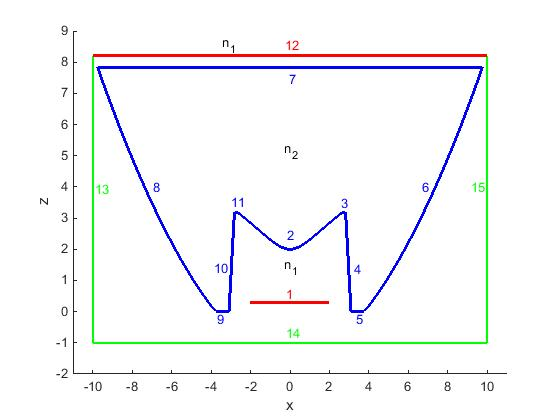
\includegraphics[width=7.7cm]{TIR}
  \end{center}
  \caption{Shape of the TIR-collimator. Each surface of the system is labeled with a number.
   The shape of the collimator is shown with a blue line.
   Three detectors depicted with green lines (surfaces $13$, $14$, and $15$) are located at the left, the right and the bottom of the optical system.
The sagitta of the lens is approximately $1.17$}
  \label{fig:tir}
\end{figure}
\\ \indent
Using PS ray tracing explained in Section \ref{sec:PS_raytracing} with parameters $\varepsilon_{\variabile{q}_1}^{\textrm{max}} = 0.1$, $ \varepsilon_{\variabile{p}}^\textrm{max} = 5\cdot 10^{-2}, $ $\varepsilon_{\variabile{q}}^\textrm{min} = 9\cdot 10^{-3}$ and $\varepsilon_\variabile{p}^\textrm{min} = 4.5 \cdot 10^{-3}$, around $1.9 \cdot 10^4$ rays are traced. 
We discard rays with direction parallel to the source, therefore $\variabile{p}_1 \in [-0.99, 0.99]$. The ray distribution at the source PS \set{S}{}{} is shown in Figure \ref{fig:sourcePS}, where we depicted with the same color the rays that follow the same path. Seven different paths are found. The yellow rays follow path $\Pi_1 = (1, 2, 7, 12)$;
   the red rays follow path $\Pi_2 ~= ~(1, 10, 8, 7, 12)$; the green rays follow path $\Pi_3 = (1, 4, 6, 7, 12)$;
   the blue rays follow path $\Pi_4= (1, 11, 7, 12)$ and the magenta rays follow path $\Pi_5= (1, 3, 7, 12)$. The rays located inside the white areas correspond to rays that do not reach the target, they follow either path $\Pi_6 = (1, 10, 7, 8, 13)$ or path $\Pi_7 = (1,4,7,6,15)$ and they do not give any contribution to the target intensity.
\begin{figure}[h]
  \begin{center}
  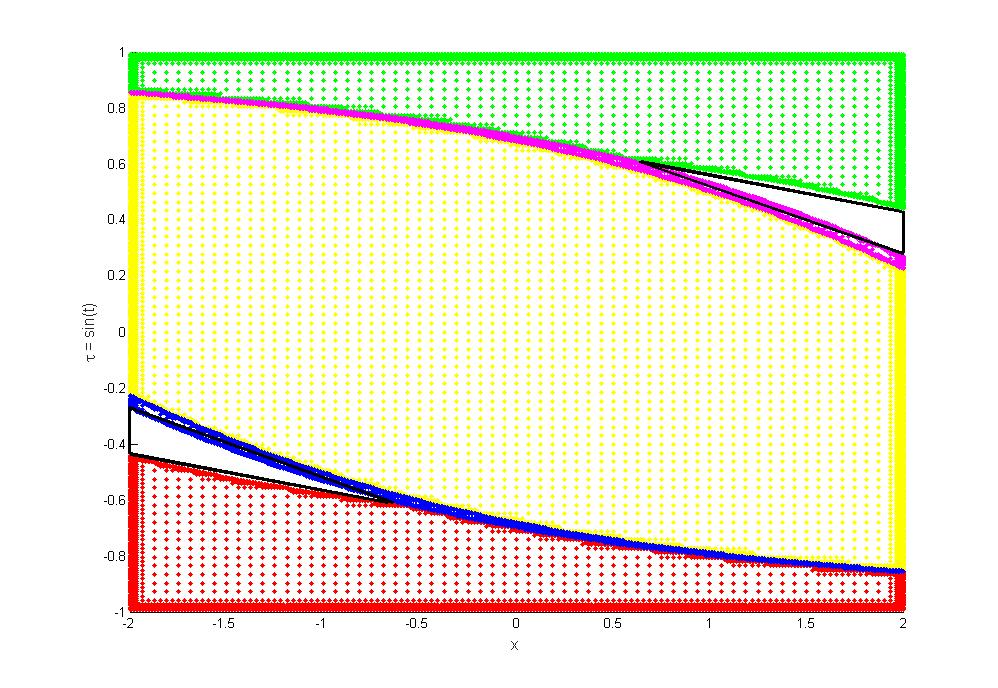
\includegraphics[width=7.7cm]{source1}
  \end{center}
  \caption{Distribution of the rays on \point{S}{}{}. Around $1.9 \cdot 10^4$ rays are traced using the triangulation refinement with parameters:
  $\varepsilon_\variabile{q}^\textrm{max} = 0.1 ,$ $ \varepsilon_{\variabile{p}}^\textrm{max} = 5\cdot 10^{-2}, $ $\varepsilon_{\variabile{q}}^\textrm{min} = 9\cdot 10^{-3}, \varepsilon_\variabile{p}^\textrm{min} = 4.5 \cdot 10^{-3}$. Rays that belong to the same region are depicted with the same color. The rays located inside the white areas do not reach the target. The boundaries of the two white regions are approximated by triangles depicted with black lines.}
  \label{fig:sourcePS}
\end{figure}
Note that, given two adjacent paths the regions $\mbox{\set{R}{$1$}{}}(\Pi)$ in \set{S}{}{} have usually a common boundary. 
Since for this system not all the rays emitted by the source arrive to the target, the target \'{e}tendue $U_{\textrm{t}}$ needs to be compared with the \'{e}tendue $U_1$ at the source given by only those rays that reach the target (the rays that follow paths $\Pi_6=(1,10,8,7,12)$ and 
$\Pi_7 = (1,4,7,6,15)$ are discarded). To this purpose $U_1$ is calculated by removing from the total area $U$ of \set{S}{}{} those areas occupied by the regions formed by the rays that hit the left and the right detector (white regions in Figure $\ref{fig:tir}$).  For the TIR collimator in Figure \ref{fig:tir}, the total source  \'{e}tendue obtained from Equation (\ref{eq:etenduesource}) is
 \begin{equation}U = 4\cdot 1\cdot 2\cdot 0.99 = 7.92.\end{equation} Indicating with $A_{T}$ the area of each white region  in Figure $\ref{fig:tir}$, $U_1$ can be approximated by:
 \begin{equation}\label{eq:Usource}
 U_{1} = 7.92-2A_{T}\approx 7.77,
 \end{equation}
 where $A_{T}$ is the approximated the area of the triangles shown in Fig. \ref{fig:sourcePS} with black lines.\\ \indent  $U_{\textrm{t}}$ is calculated several times from Equation (\ref{eq:etenduetarg}) where every time the boundaries $\partial$\set{R}{}{}$(\Pi)$ are obtained by using $\alpha$-shapes for a different value of $\alpha$. A better approximation of $\partial$\set{R}{}{}$(\Pi)$ gives a value of $U_{\textrm{t}}$ closer to the exact \'{e}tendue. 
Matching $U_1$ with all the approximation of $U_{\textrm{t}}$ we find the best value $\alpha_c$ of $\alpha$ that approximates $\partial$\set{R}{}{}$(\Pi)$ and, therefore, $U_{\textrm{t}}$. \\ \indent In Figure \ref{fig:etendueTS} we represent the approximated value of the source \'{e}tendue $U_1\approx 7.77$ with the dotted red line obtained from Equation (\ref{eq:Usource}). Different approximations of the target \'{e}tendue $U_{\textrm{t}}$ are calculated using Equation (\ref{eq:etenduetarg1}) where every time the boundaries $\partial$\set{R}{}{}$(\Pi)$ are found using $\alpha$-shapes for a different value of $\alpha$. In Figure \ref{fig:etendueTS}, we show how the \'{e}tendue change by increasing the value of $\alpha$. This graph shows that using PS ray tracing with $1.67\cdot 10^4$ rays, the best approximation of the boundaries $\partial$\set{R}{}{}$(\Pi)$ is given considering $\alpha = \alpha_c = 0.139$ in the $\alpha$-shapes procedure.
 \begin{figure}[h]
  \begin{center}
  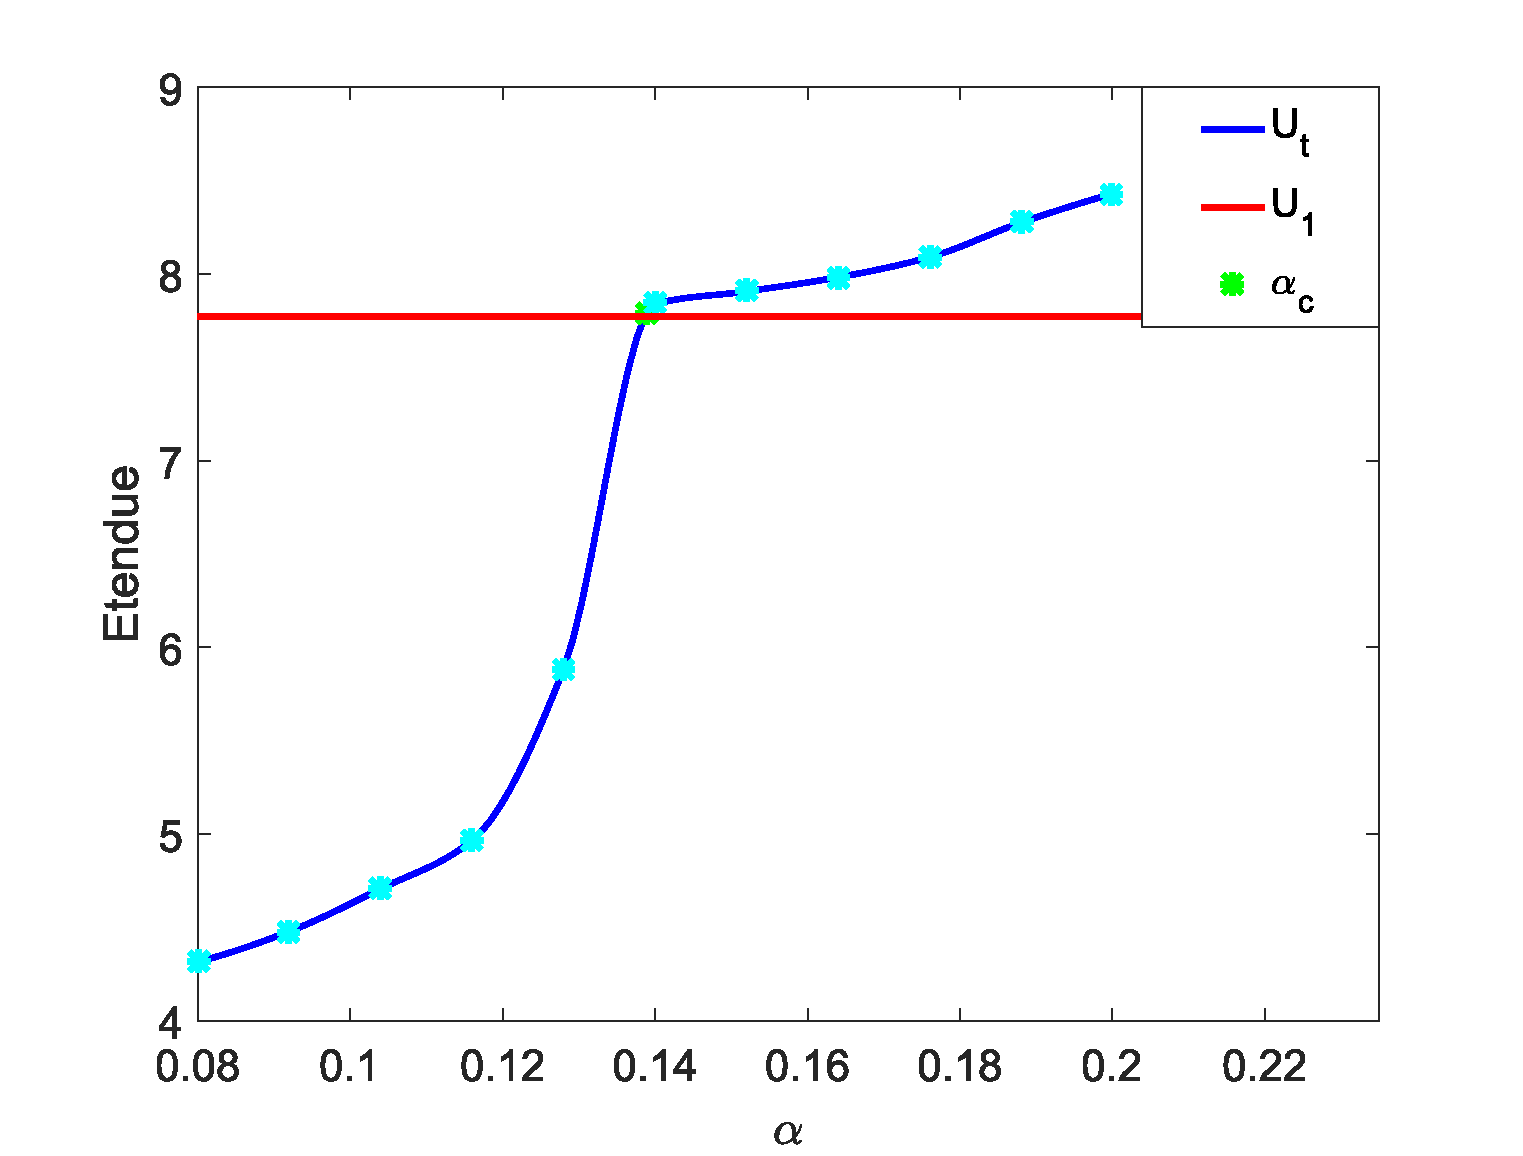
\includegraphics[width=7.7cm]{etendue_alpha}
  \end{center}
  \caption{\footnotesize{The source and the target \'{e}tendue are depicted with the red line and the blue line, respectively.
  $U_\textrm{t}$ is computed for a range of values for $\alpha$. $U_1 \approx 7.77$
   The green dot indicates the value of $\alpha_c = 0.139$ which gives the best approximation of the boundaries $\partial$\set{R}{}{}$(\Pi)$ at the target.
   Around $1.67 \cdot 10^4$ rays have been traced using PS ray tracing.
  }}
  \label{fig:etendueTS}
\end{figure}
Applying $\alpha$-shapes with $\alpha=\alpha_c$, a good approximation of $\partial$\set{R}{}{}$(\Pi)$ is found. In Fugure \ref{fig:targetPS} we show the boundaries 
$\partial$\set{R}{}{}$(\Pi)$ in target PS \set{T}{}{} with $\alpha_c=0.041$ and tracing $1.9\cdot10^4$ rays.
  \begin{figure}[h]
  \begin{center}
  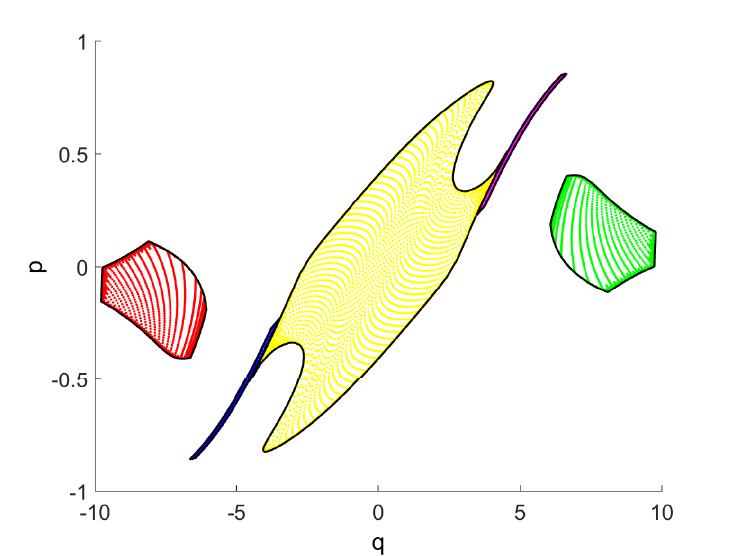
\includegraphics[width=7.7cm]{target_alpha_shapes.png}
  \end{center}
  \caption{\footnotesize{Target PS representation of a set of $1.67 \cdot 10^4$ rays.
  Rays that follow the same path are depicted with the same color. The choice of the colors for each path is the same as in Figure $\ref{fig:sourcePS}$. The boundaries $\partial$\set{R}{}{}$(\Pi)$ are computed through the $\alpha$-shapes method with $\alpha = \alpha_c = 0.139$.}}
  \label{fig:targetPS}
\end{figure}
Once the boundaries are computed, the target intensity $I_{\textrm{PS}}(\variabile{p})$ for every $\variabile{p}\in[-1,1]$ is obtained from Equation (\ref{eta2}). \\ \indent
To validate our method we compare the PS intensity with the MC intensity. 
To this purpose a partitioning $P_2:-1=\variabile{p}_{0}<\variabile{p}_1<\cdots<\variabile{p}_{\nbin}=1$ of the interval $[-1,1]$ into $\nbin=100$ bins is considered. 
The averaged and normalized PS intensity $\hat{I}_{\textrm{PS}}$ is calculated for every 
$\big(\variabile{p}^{\variabile{h}+1/2} = \frac{1}{2}(\variabile{p}^{\variabile{h}+1}+ \variabile{p}^{\variabile{h}})\big)_{\variabile{h}=0, \cdots, \nbin-1}$ dividing the PS averaged intensity by the total \'{e}tendue:
\begin{equation}\label{eq:normalized_PS_intensity}
\hat{I}_{\textrm{PS}}(\variabile{p}^{\variabile{h}+1/2}) = \frac{1}{U_{\textrm{t}}}\int_{\variabile{p}_{\variabile{h}}}^{\variabile{p}_{\variabile{h}+1}} I_{\textrm{PS}}(\variabile{p})\textrm{d}\variabile{p}
\end{equation}
The averaged and normalized MC intensity $\big(\hat{I}_{\textrm{MC}}(\variabile{p}^{\variabile{h}+1/2})\big)_{\variabile{h} = 0, \cdots, \nbin-1}$ intensity is given by
\begin{equation}\label{eq:normalized_MC_intensity}
\hat{I}_{\textrm{MC}}(\variabile{p}^{\variabile{h}+1/2}) = \frac{\nrays[\variabile{p}^{\variabile{h}-1},\variabile{p}^{\variabile{h}})}{\nrays[-1,1)} 
\qquad \mbox{ for } \variabile{p}\in[\variabile{p}^{\variabile{h}-1}, \variabile{p}^{\variabile{h}}).
\end{equation} 
Both the approximate intensities $\hat{I}_{\textrm{A}} (\textrm{A} = \textrm{PS}, \textrm{MC})$ are compared with an intensity $\hat{I}_{\textrm{ref}}$ taken as a reference. For some optical systems, there is an explicit solution for the target intensity but this is not the case of the TIR-collimator.
Therefore, a MC simulation with $1.7 \cdot 10^8$ rays is run to obtain the averaged normalized intensity $\hat{I}_{\mbox{ref}}$ which is used as reference.
The intensity profile $\hat{I}_{\textrm{PS}}
$ obtained using PS ray tracing with $66\,855$ rays and $\alpha= \alpha_c = 0.02$ is depicted in Fig. \ref{fig:intensityMCPS} with a red line.
$\hat{I}_{\textrm{PS}}$ is hardly distinguishable from $\hat{I}_{\mbox{ref}}$ (dashed and blue line in Figure $\ref{fig:intensityMCPS}$).\\ \indent
  \begin{figure}[h]
    \centering
    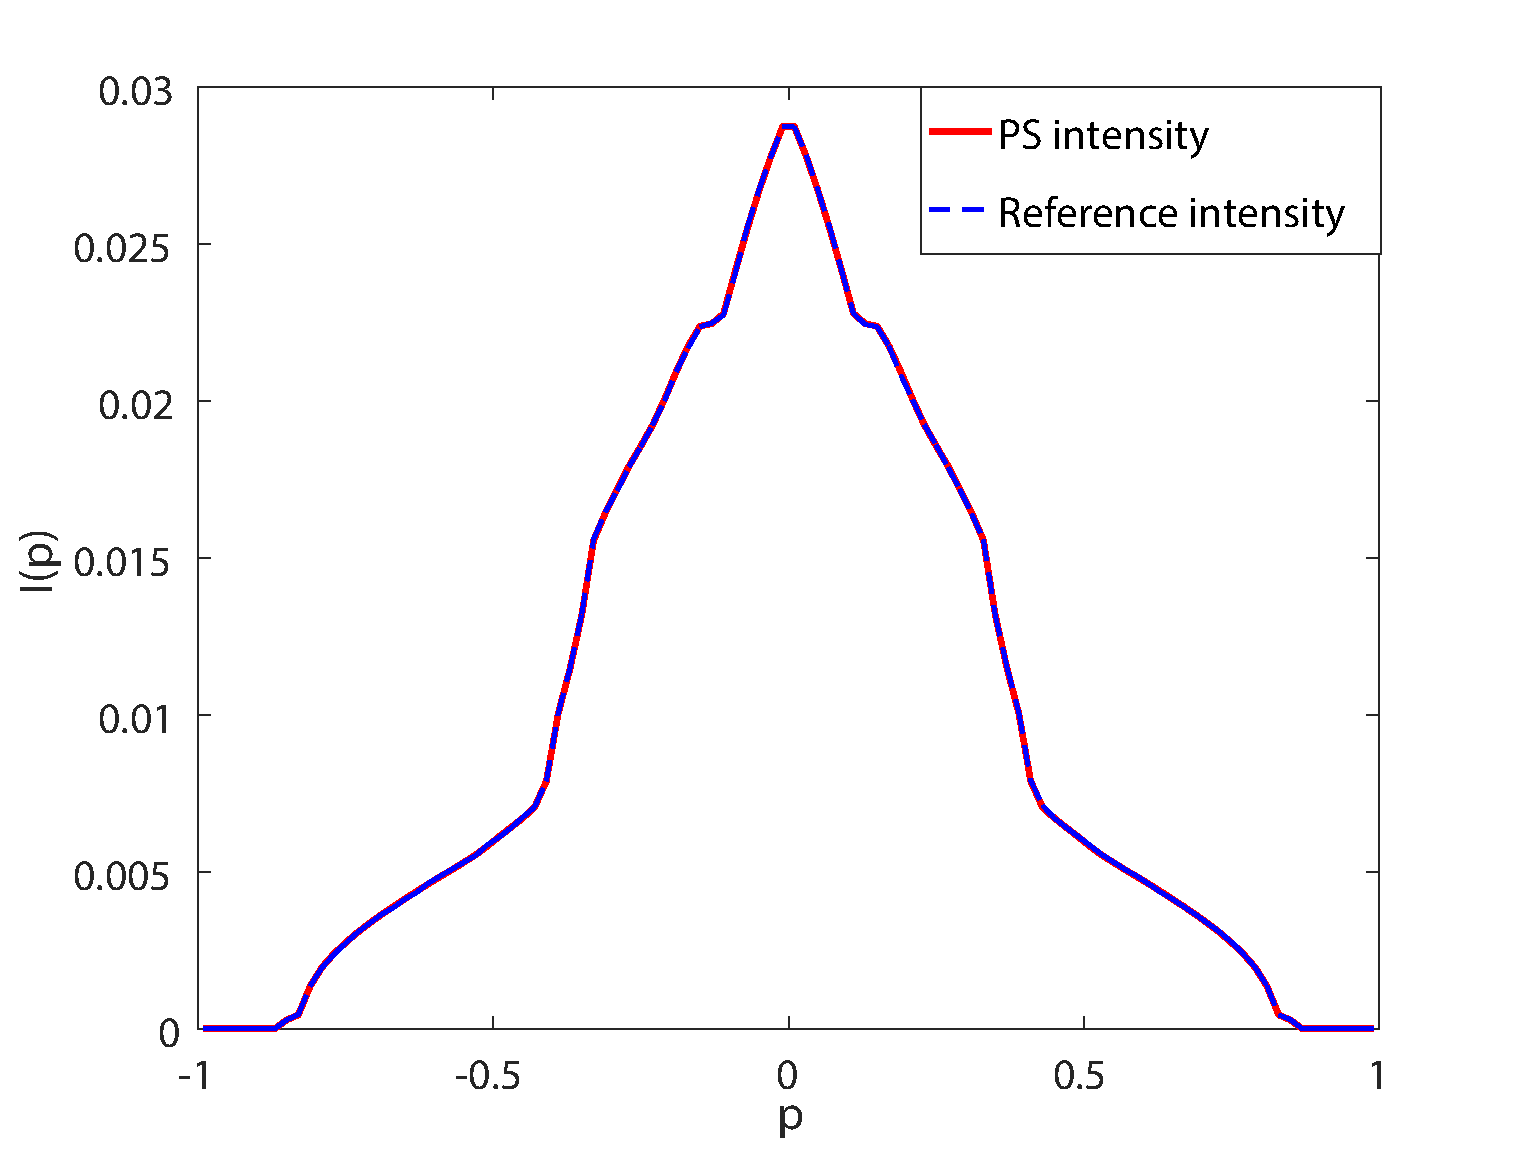
\includegraphics[width=7.7 cm]{intensity_alpha_shapes}
\caption{The red line shows the PS intensity at the target of the TIR-collimator. The exact intensity is depicted with the dotted blue line.
The exact intensity is computed using the MC method for a set of $15$ millions of rays. For the PS intensity a set of $6.6\cdot 10^4$
rays is considered and $\alpha_c = 0.02$ is chosen to compute the boundaries $\partial$\set{R}{}{}$(\Pi)$. The approximate intensity can hardly be distinguished from the reference intensity.}
  \label{fig:intensityMCPS}
\end{figure}
Finally, we calculate the error between $\hat{I}_{\textrm{A}}$ and $\hat{I}_{\textrm{ref}}$, defined as:
\begin{equation}\label{eq:error}
\mbox{error} = \frac{\sum_{\variabile{h}= 1}^{\nbin}| \hat{I}_{A}(\variabile{p}^{\variabile{h}}) - \hat{I}_{\mbox{ref}}(\variabile{p}^{\variabile{h}})|}{\nbin}.
\end{equation}
The MC and PS intensities are calculated several times increasing the number of rays to improve the accuracy.
Tables \ref{tab:table} and \ref{tab:table2} describe how the number of rays traced affects the error. 
In Table \ref{tab:table} a correlation between $\alpha_c$ and the number of rays is shown.
%determined by the values of $\varepsilon^{\textrm{min}}_\variabile{p}$, $\varepsilon^{\textrm{min}}_{\variabile{q}}$, 
%$\varepsilon^{\textrm{max}}_{\variabile{p}}$ and $\varepsilon^{\textrm{max}}_{\variabile{q}}$. 
Note that increasing the number of rays the value of $\alpha_c$ and the corresponding error decrease. 
\begin{table}[htbp] \label{tab:table}
\centering
\caption{\bf Error values of the PS intensity}
\begin{tabular}{lllllll}

 \hline  Number \\ of rays\;  & $\varepsilon^{\textrm{max}}_{\variabile{q}} $  & $\varepsilon^{\textrm{min}}_{\variabile{q}} $   \;     & $\varepsilon^{\textrm{max}}_{\variabile{p}}$\;
  & $\varepsilon^{\textrm{min}}_\variabile{p}$\; & $\alpha_c$  & PS error \\
  \hline 
 $3\,363$ & $0.9$  & $0.1$  & $0.50$  & $0.025$ & $0.119$ & $1.20\cdot10^{-3}$ \\
$6\,949$  & $0.5$  & $0.050$  & $0.25$  & $0.020$ & $0.098$ & $2.50\cdot 10^{-4}$  \\
$15\,870$  & $0.4$  & $0.025$  & $0.02$  & $0.001$ & $0.050$ & $5.49\cdot 10^{-5}$ \\
 $37\,455$  & $0.2$  & $0.020$  & $0.10$ & $0.005$ & $0.037$ & $2.00\cdot 10^{-5}$ \\
 $66\,855$ & $0.1$  & $0.009$  & $0.05$  & $0.004$ & $0.020$ & $1.00\cdot 10^{-5}$ \\
 \hline
 \end{tabular}
 \label{tab:table}
 \end{table}
\\ \indent In Table \ref{tab:table2} the numerical results of MC ray tracing are reported.
Increasing the number of rays traced in MC ray tracing, the error gradually decreases.
\begin{table}[htbp]
\centering
\caption{\bf Error values of the MC intensity}
\begin{tabular}{ll} \hline   Number of rays\; & MC error\\ \hline $972$  & $2.10\cdot10^{-3}$ \\
$9\,714$  & $6.69\cdot 10^{-4}$  \\ $97\,103$  & $2.08\cdot 10^{-4}$ \\ $971\,627$  & $7.00\cdot 10^{-5}$ \\ $9\,716\,519$  & $2.00\cdot 10^{-5}$ \\
 \hline
 \end{tabular}
 \label{tab:table2}
 \end{table}
\noindent In Figure $\ref{fig:error}$, the results listed in Table $\ref{tab:table}$ and Table $\ref{tab:table2}$ are shown. The red line depicts the convergence of the PS error and the blue line indicates the MC error.
\begin{figure}[h!]
  \begin{center}
  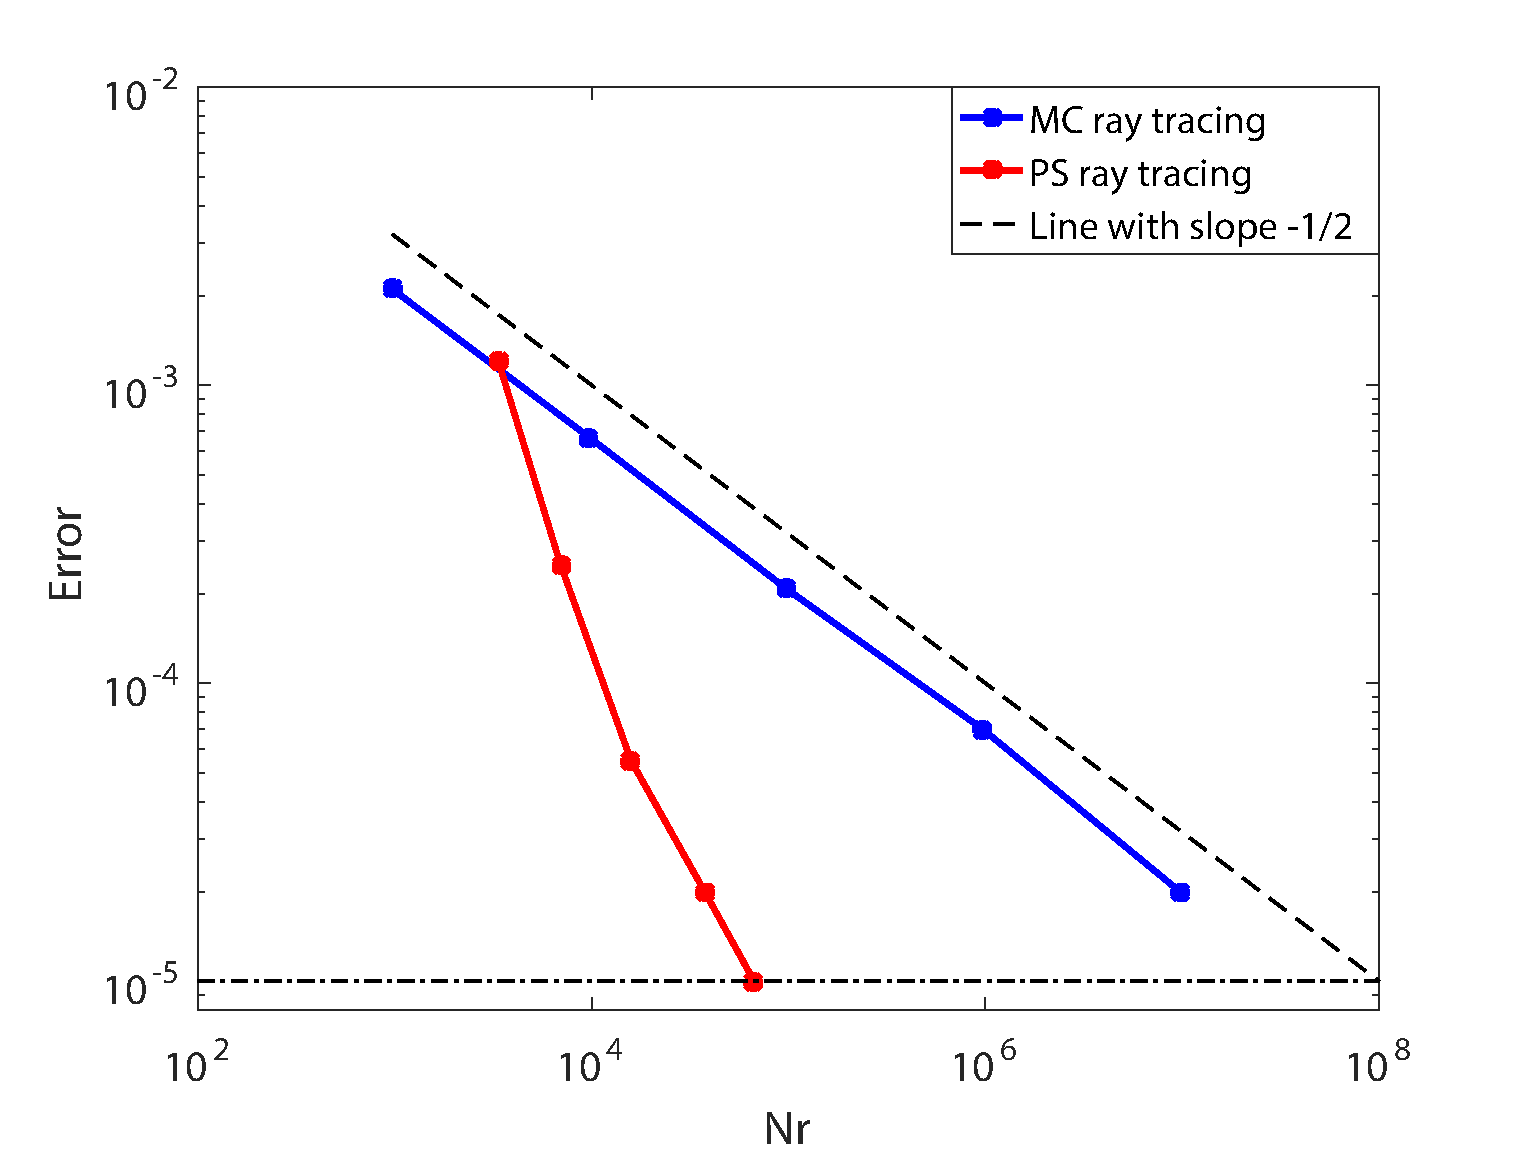
\includegraphics[width=7.7cm]{error_alpha_shapes1}
  \end{center}
  \caption{ The red line depicts the error between the PS intensity and the reference intensity.
 The blue line shows the error between the MC intensity and the reference intensity.
  The dashed line represents a straight line with the slope equal to $-\frac{1}{2}$.
  The horizontal dotted line shows that an error equal to $2.00 \cdot  10^{-5}$ can be obtained tracing at least $10^2$ times fewer rays in phase space.}
  \label{fig:error}
\end{figure}
Note from Figure \ref{fig:error} that the error for the MC method decreases as $\frac{1}{\sqrt{\nrays}}$, while for the PS simulation the speed of convergence is much higher.\\ \indent
We need to emphasize that the PS ray tracing convergence may change according to the design of the optical system.
This is because the approximation of the boundaries in PS depends on the accuracy of the $\alpha$-shapes method.
The $\alpha$-shapes is unable to properly detect the boundaries of regions with a sharp turn if not enough points are given
\cite{teichmann1998surface}. Indeed, on the one hand a low density requires a big values of $\alpha$ to accept the triangles in a region, on the other hand,
 choosing $\alpha$ big, the shape of the region could be destroyed (some rays inside the regions could be taken into account).
\begin{figure}[h]
\centering
\begin{subfigure}{.48\textwidth}
  \centering
  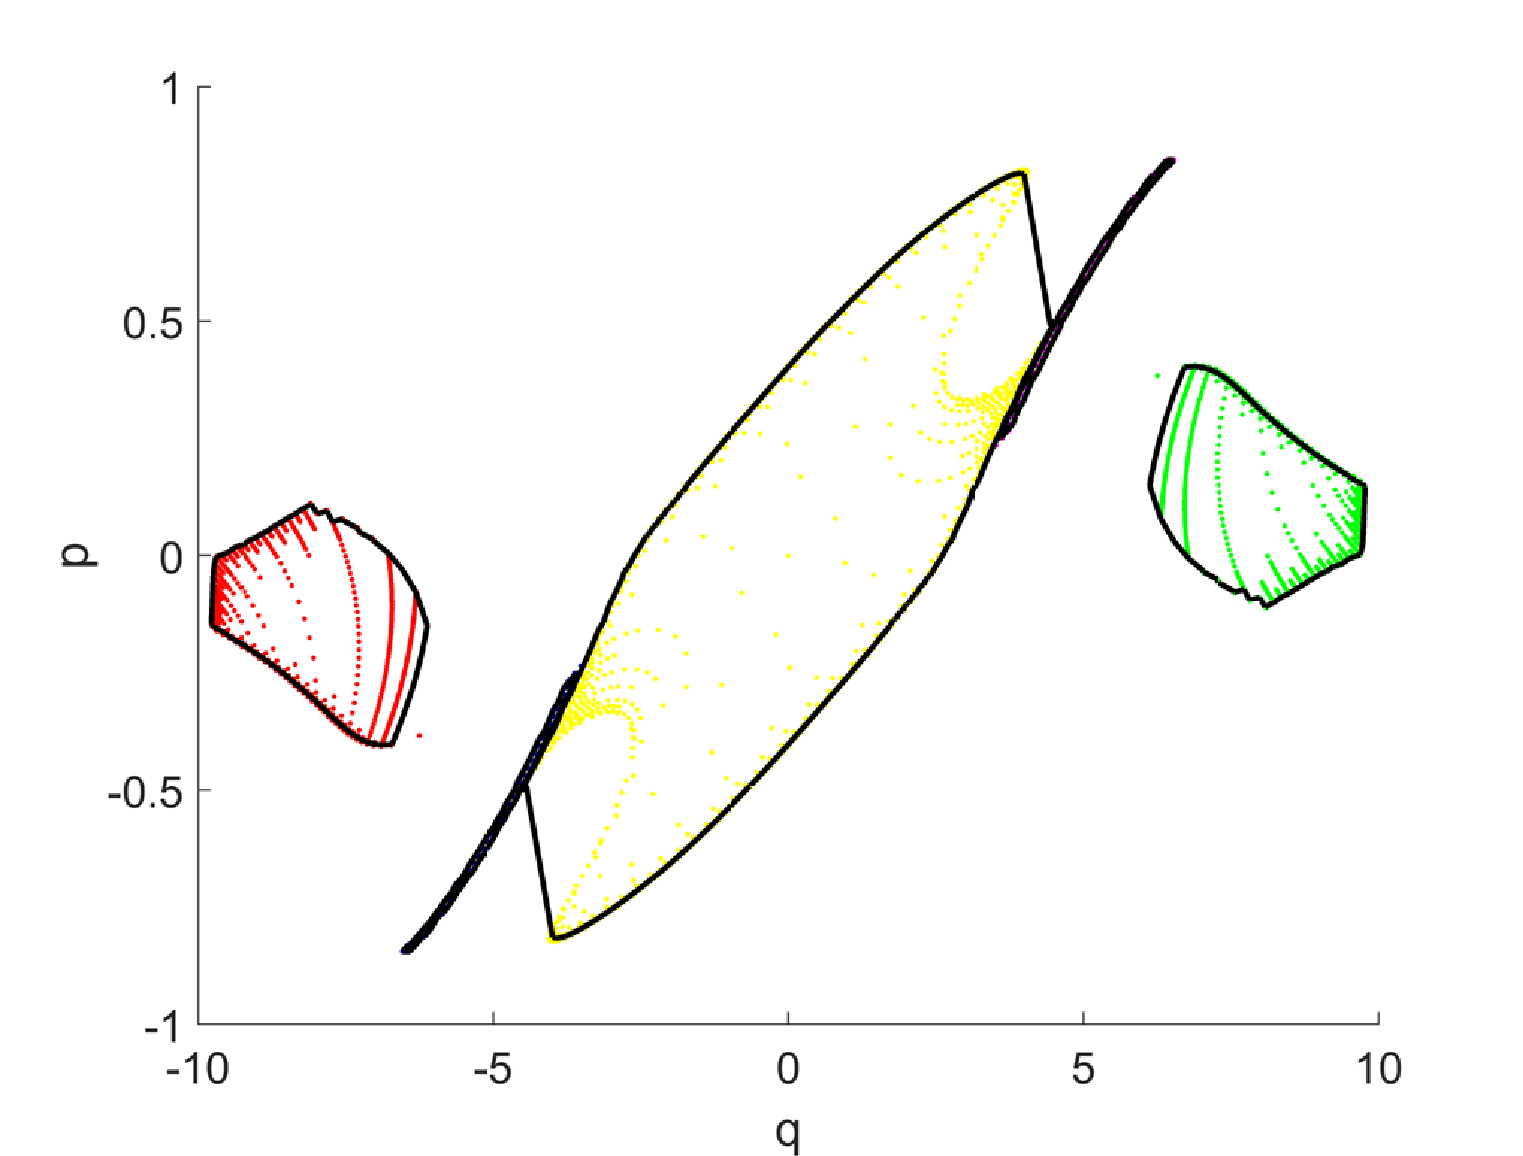
\includegraphics[width=\textwidth]{boundaries_alpha1}
  \caption{Boundaries approximation obtained using the $\alpha$-shapes method with $\alpha_c = 0.3$ (black line).}
\end{subfigure}
\begin{subfigure}{.48\textwidth}
  \centering
  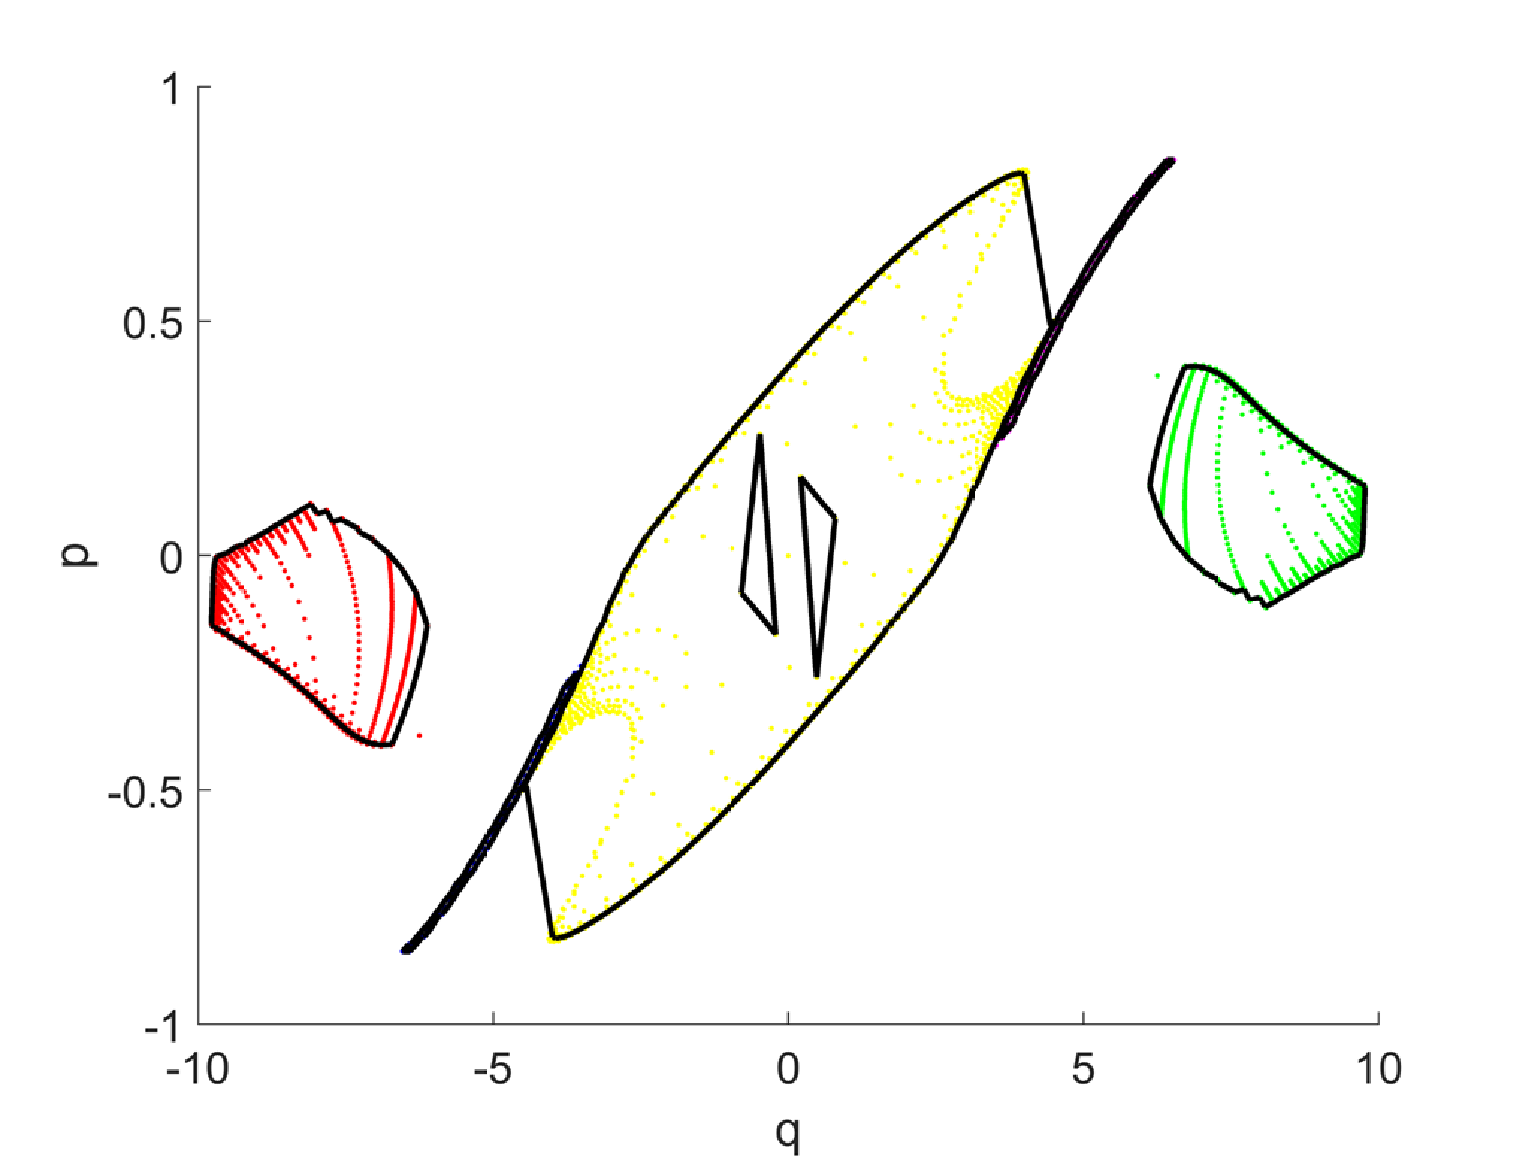
\includegraphics[width=\textwidth]{boundaries_alpha2}
  \caption{Boundaries approximation obtained using the $\alpha$-shapes method with $\alpha_c = 0.31$ (black line).}
\end{subfigure}
\caption{Boundaries approximation of the regions with positive luminance at the target PS. Tracing $3339$ rays and using $\alpha$-shape the boundaries cannot be approximated well. 
A small change of the parameter $\alpha$ leads to a completely different approximation of the boundaries.}
\label{fig:Tir1}
\end{figure}
%\centering
%  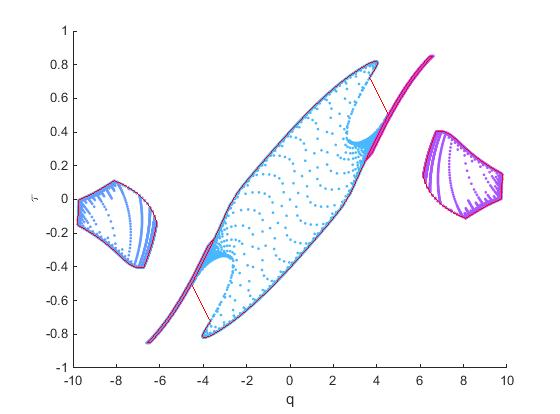
\includegraphics[width=7.7cm]{Tir1}
%    \caption{Target PS for the TIR-collimator depicted in
%    Figure \ref{fig:tir}. The red line depicts the best approximations of $\partial$\set{R}{}{}$(\Pi)$ for $3363$ rays with $\alpha_c = 0.119$.
%    The cyan region in the middle of the target PS is formed by rays that hit the lens, it is hard to approximate that region when there is a small number of rays inside it.}
%     \label{fig:Tir1}
%  \end{figure}
Figure $\ref{fig:Tir1}$ clarifies this concept showing that the region formed by rays that hit the lens is hard to approximate when there is a small number of rays inside the region. Consequently either a region bigger than the area covered by the rays is considered or some triangles which are not part of the boundaries are considered in the triangulation. This results in an inaccurate calculation of the intensity (either too high or to low). To obtain a good approximation of the boundaries of these kind of patches more rays have to be traced. Therefore, the error in the approximate intensity is relatively big for few rays (compared to MC error) and it decreases very fast increasing the number of rays (see Table
 \ref{tab:table} and Figure \ref{fig:error}).
 \\\indent To show how the error plot changes according to the regularity of the shape of the regions $\partial$\set{R}{}{}$(\Pi)$, we consider another example of TIR-collimator.
 Figure $\ref{fig:Tir1}$ shows that the hardest region to approximate is given by those rays that follow path $\Pi_1 ~=~ (1,2,7,12)$.
 We therefore consider a TIR-collimator with a flatter lens and with the target located at a closer distance from the top (see Figure $\ref{fig:analyticlens}$). 
The source $\mathcal{S}= [-2,2]$ (surface number $1$) is located in air at a height $\variabile{z}_1 = 0.3$ from the $x$-axis.
       The target $\mathcal{T}= [-9.7, 9.7]$ (surface $12$) is parallel to the source and is located in air at a height $ \variabile{z}= 7.85$.
       The shape of the collimator is shown as a blue line.
       Three detectors depicted with green lines (surfaces $13$, $14$, and $15$) are located at the left, the right and the bottom of the optical system.
 \\ \indent Tracing around $3363$ rays using PS ray tracing, we obtain the target rays distribution shown in Figure $\ref{fig:Tir2}$. 
Note that a flatter lens removes one of the two spikes of the region formed by the rays that hit the lens.
Moreover a target located very close to the top makes the shape of that region less stretched along the $\variabile{q}$-axis.
Therefore, it is expected that $\alpha$-shapes method performs well, even for a small number of rays.
\begin{figure}[h]
  \begin{center}
  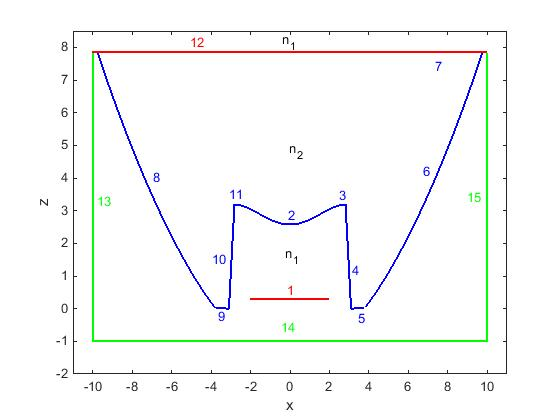
\includegraphics[width=6.5cm]{tir_analytic2}
   \end{center}
    \caption{Shape of the TIR-collimator. Each surface of the system is labeled with a number.
%       The source $\mathcal{S}= [-2,2]$ (surface number $1$) is located at a height $\variabile{z}_1 = 0.3$ from the $x$-axis.
%       The target $\mathcal{T}= [-9.7, 9.7]$ (surface $12$) is parallel to the source and is located at a height $ \variabile{z}= 7.85$.
%       The shape of the collimator is shown as a blue line.
%       Three detectors depicted with green lines (surfaces $13$, $14$, and $15$) are located at the left, the right and the bottom of the optical system.
       $n_1 = 1$ is the refraction index of the medium (air) where the source and the target are located, and
       $n_2 = 1.5 $ the refraction index of the medium (glass) inside the optical system. The sagitta of the lens is equal to $0.6$}
 \label{fig:analyticlens}
\end{figure}
 \begin{figure}[h]
  \begin{center}
       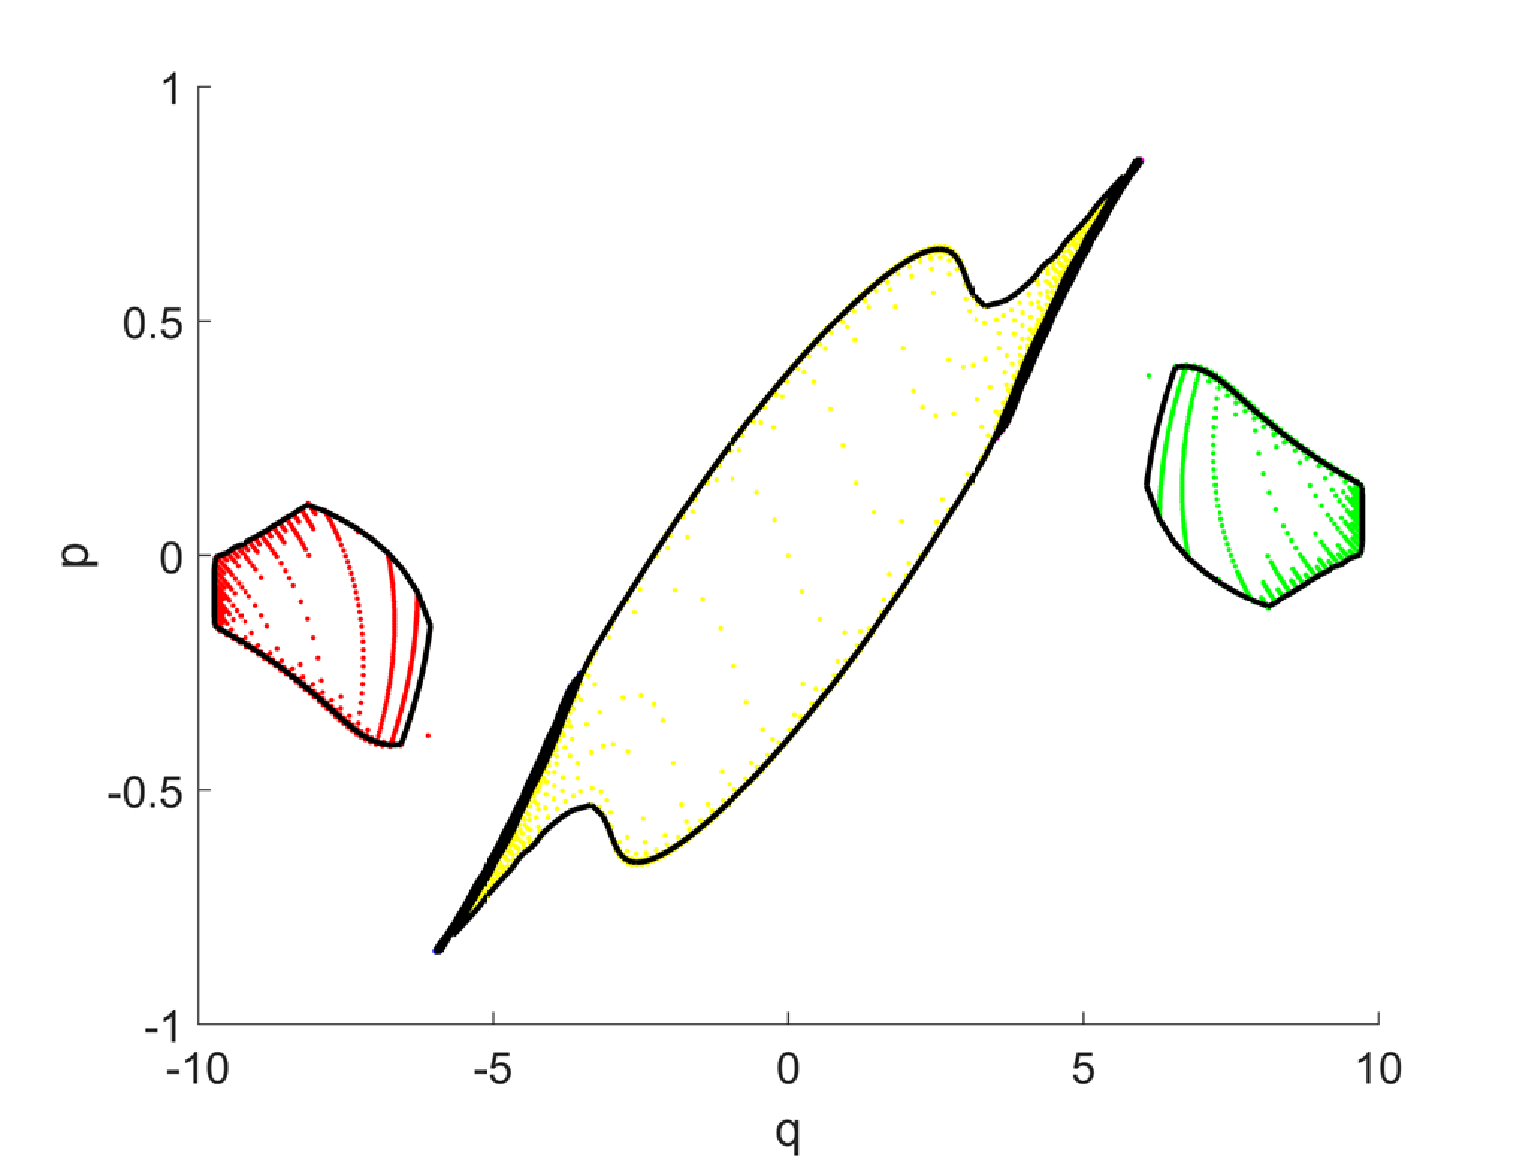
\includegraphics[width=7.7cm]{boundaries_alpha3}
   \end{center}
        \caption{Target phase space for the TIR-collimator depicted in
        Figure \ref{fig:analyticlens}. The black line depicts the best approximation of $\partial$\set{R}{}{}$(\Pi)$ for $3281$ rays. 
The $\alpha$-shapes method gives an accurate approximation of the boundaries for $\alpha_c = 0.9$.}
  \label{fig:Tir2}
\end{figure}
\\ \indent PS and MC ray tracing are implemented for the TIR-collimator in Figure \ref{fig:Tir2}. The approximated intensities $\hat{I}_{\textrm{A}}$ $(\textrm{A} = \textrm{PS}, \textrm{MC})$ are compared with the reference intensity $\hat{I}_{\textrm{ref}}$ (MC ray tracing with $10^7$ rays). The error between $\hat{I}_{\textrm{A}}$ and $\hat{I}_{\textrm{ref}}$ as a function of the number of rays is obtained from Equation (\ref{eq:error}). The convergence of PS and MC ray tracing is shown in Figure \ref{fig:error2}. 
PS error is depicted with the red line and, MC error is depicted with the blue line.\\ \indent
For the TIR-collimator in Figure \ref{fig:analyticlens} we obtained a speed of convergence of the order of $O\big(\frac{1}{\nrays}\big)$ for PS ray tracing versus an order of convergence of $O\big(\frac{1}{\sqrt{\nrays}}\big)$ for MC ray tracing.
\begin{figure}[h!]
 \begin{center}
   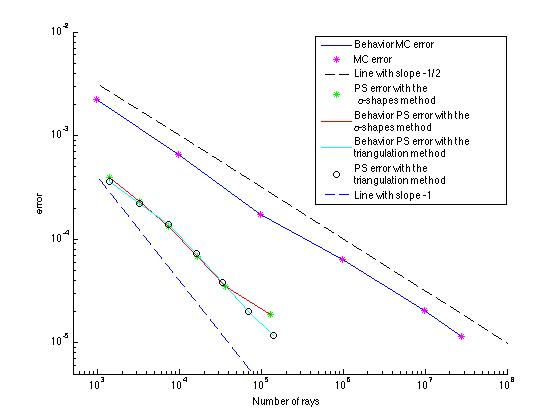
\includegraphics[width=7.7cm]{error_plot}
    \end{center}
     \caption{The red line depicts the error using the $\alpha$-shapes method to compute the boundaries. The cyan line depicts the error using the triangulation refinement to compute the boundaries.
     The blue line shows the error between the Monte Carlo intensity and the exact intensity.
     The dashed black line represents a straight line with slope $-\frac{1}{2}$.
   The dashed blue line represents a straight line with slope $-1$.}
 \label{fig:error2}
\end{figure}
\section{Conclusion}
The aim of this chapter was to detect the boundaries of the regions formed by the rays traced using $\alpha$-shapes.\\
\indent First, we reported some theory about $\alpha$-shapes methods which are common used to approximate the shape formed by a point cloud. 
These methods depend on a parameter $\alpha$ that in most cases can be determined only by several simulations. 
\\ \indent Using \'{e}tendue conservation, we developed a new approach to detect the value of $\alpha$ that better approximates the boundaries in target PS. 
We applied $\alpha$-shapes to two different kinds of TIR-collimators. The target PS intensity was computed for both the systems several times increasing every time the number of rays traced. Finally, the corresponding errors between the intensities found and a reference intensity was calculated. We observed that PS ray tracing leads to trace far less rays compared to MC ray tracing. Numerical results show that using PS ray tracing the desired accuracy can be achieved reducing the number of rays traced by a factor $2$ for both the optical systems analyzed.\\ \indent 
However, we observed that the error convergence for PS ray tracing strongly depends on the design of the optical system (shapes of the region in target PS). Indeed, the intensity accuracy is related to the precision of the $\alpha$-shape, that is, to the choice of the parameter value of $\alpha$. For more complicated shapes in PS, more rays need to be traced for a good boundaries reconstruction.\\ \indent
In order to remove the dependence of PS ray tracing from the parameter $\alpha$, we construct another procedure to detect the boundaries of the regions in target PS. 
The new technique is based on the triangulation refinement explained in Section \ref{sec:PS_raytracing}. The details are explained in the next chapter and numerical results are reported for several optical systems. 












































\chapter{The inverse ray mapping method: analytic approach}\label{chap:raymapping1}
%Employing the source and the target PS of the optical systems an improvement of MC and QMC ray tracing was presented in the previous chapters.
In this chapter a new method that employs not only the source and the target PS but also the PS of \textit{all} the other lines that constitute the optical system is introduced. %Furthermore, instead of starting from the source, the new approach is an inverse method which starts considering rays on target PS.
All lines can be modeled as detectors of the incident light and emitters of the reflected light.
Moreover, we assume that the source can only emit light and the target can only receive light.
Therefore, one PS is taken into account for the source and one for the target while both the source and target phase spaces are considered for the other lines. Every line of the system (except for the source \point{S} and the target \point{T}) constitutes
the target for incident rays and the source for reflected rays. Therefore, two different phase spaces are considered for the reflectors and one PS for
\point{S} and \point{T}. All these phase spaces are connected through a map which relates the rays coordinates on every PS. In order to compute the target photometric variables an inverse ray mapping reconstruction from the target to the source is involved.
\\\indent
In this chapter two different optical systems are investigated.
First, the method is explained for the two-faceted cup. 
Then, it is extended to a more complicated system, the so-called multi-faceted cup, which is formed by only straight lines segments.
\section{Explanation of the method}
%Theonstructing a map from the source to the target of the system. This map can be written as the concatenation of many maps which
%%can be classified as two different kinds of maps, i.e. the map that connects the source and the target PS of two \textit{different} lines and the map that connects the target and the source PS of the \textit{same} line.
%%Employing the inverses of these maps we are able to detect the parts on target PS illuminated by the source.
% All the rays in PS are connected trhough a map
%All the PS considered are divided into regions, the boundaries of which can be determined exactly for systems formed by straight lines.
%We make the assumption of a Lambertian source; hence, the luminance is a positive constant when different from $0$. 
%As a consequence, the output intensity along a given direction is given by the total width of all the patches with positive luminance, measured along that direction.\\ \indent
\section{The two-faceted cup}
A two-faceted cup is

%\section{The multi faceted cup}
%For two-dimensional systems every ray in the PS of a line is given by a two-tuple point. Therefore, the PS of every line is a two-dimensional space.
%The position coordinate in the PS of line \variabile{i} is the \variabile{x}-coordinate of the intersection point between the ray and the line \variabile{i}.
%The direction coordinate is the sine of the angle that the ray forms with respect to the normal of the line \variabile{i} multiplied by the index of refraction of the medium in which the ray is located.
%Let's now introduce some notation before explaining the details of the method. We indicate the PS with $\set{S}{}{}=\set{Q}{}{}\times\set{P}{}{}$,
%where $\set{Q}{}{}$ is the set of the position coordinates \variabile{q} and $\set{P}{}{}$ is the set of the direction coordinates $\variabile{p}=\variabile{n}\sin{\tau}$ with $\tau$ the angle between the ray and the normal \textit{$\boldsymbol{\nu}$} of the line and \variabile{n} is the index of refraction of the medium in which the line is located.  
%The normal \vect{$\boldsymbol{\nu}$} is always directed into the cup and the angle $\tau$ between the ray and \vect{$\boldsymbol{\nu}$} is measured counterclockwise.
%In this paper we analyze only systems located in air ($\variable{n} = 1$), therefore, from now on, we do not write the index \variable{n} anymore.
%The source and the target PS of a line $\variable{i}$ are indicated with \set{S}{i}{} and \set{T}{i}{}, respectively.
The coordinates of every ray that reaches the line $\variable{i}\in\{1, 2, 3\}$ are indicated  with $(\pos{t,}{i}, \dir{t,}{i})$ on \set{T}{i}{}.
%After reflection, the ray leaves line $\variable{i}\in\{1, 2, 3\}$ at the same position and with a new direction, the new coordinates are indicated with $(\pos{s,}{i}, \dir{s,}{i})$ on \set{S}{i}{}.
%Note that $\pos{s,}{i}= \pos{t,}{i}$ while $\dir{s,}{i}$ is obtained applying the reflection law to the direction coordinate $\dir{t,}{i}$ of the incident ray.
%The phase spaces \set{S}{i}{} and  \set{T}{i}{} of each line \variable{i} are partitioned into different regions, (\set{S}{i,}{j})$_{\variable{j}=2, 3, 4}$ and (\set{T}{i,}{k})$_{\variable{k}=1, 2, 3}$, respectively, where \variable{j}$\neq$ \variable{i} is the index of the line that is illuminated by \variable{i} and \variable{k}$\neq$ \variable{i} is the index of the line that illuminates \variable{i}. Hence, we indicate with \set{S}{i,}{j} $\subset$ \set{S}{i}{} the part of \set{S}{i}{} corresponding to rays that illuminate line \variable{j} and with \set{T}{i,}{k} $\subset$ \set{T}{i}{} the part of \set{T}{i}{} corresponding to rays originating from the line \variable{k}. Note that, due to the fact that the source only emits light, we do not define its target phase space \set{T}{$1$}{}. Similarly, since the target only receives light, its source phase space \set{S}{$4$}{} is not defined.
%For the two-faceted cup, six different phase spaces need to be considered which are given by the following expressions:
 %\begin{equation}
 %S_{\textit{i}}= \bigcup_{\begin{array}{cc}\textrm{j}=2\\\textit{j}\neq\textit{i}\end{array}}^4
 %S_{\textit{i,j}}
 %\end{equation}
\begin{equation}
\label{SPS}
\begin{split}
 \mbox{\set{S}{$1$}{}} & = \mbox{\set{S}{$1$,}{$2$}}\cup
 \mbox{\set{S}{$1$,}{$3$}} \cup \mbox{\set{S}{$1$,}{$4$}},\\
\mbox{\set{S}{$2$}{}} & =  \mbox{\set{S}{$2$,}{$3$}} \cup \mbox{\set{S}{$2$,}{$4$}},\\
\mbox{\set{S}{$3$}{}} & =  \mbox{\set{S}{$3$,}{$2$}} \cup \mbox{\set{S}{$3$,}{$4$}},\\
\mbox{\set{T}{$2$}{}} & = \mbox{\set{T}{$2$,}{$1$}} \cup \mbox{\set{T}{$2$,}{$3$}},\\
\mbox{\set{T}{$3$}{}} & = \mbox{\set{T}{$3$,}{$1$}}\cup \mbox{\set{T}{$3$,}{$2$}},\\
\mbox{\set{T}{$4$}{}} & = \mbox{\set{T}{$4$,}{$1$}}\cup \mbox{\set{T}{$4$,}{$2$}}\cup
\mbox{\set{T}{$4$,}{$3$}}.
\end{split}
 \end{equation}
%% \begin{equation}
%% T_{\textit{i}}= \bigcup_{\begin{array}{cc}\textrm{k}=1\\\textit{k}\neq\textit{i}\end{array}}^3 T_{\textit{i,k}}\;.
%% \end{equation}
%We need to note that, as the source cannot receive light and the target cannot emit light,  the regions $(\mbox{\set{S}{i,}{$1$}})_{\variable{i}=2,3}$ and $(\mbox{\set{T}{i,}{$4$}})_{\variable{i}=2, 3}$ are not considered.
%The boundaries $\partial \mbox{\set{S}{i,}{j}}$ are mapped into the boundaries $\partial \mbox{\set{T}{j,}{i}}$ for every $\variable{i}=\{1, 2, 3\}$ 
%and $\variable{j}=\{2, 3,4\}$ with $\variable{j}\neq \variable{i}$ (edge-ray principle \cite{Ries}). For the two-faceted cup and for all systems that are formed by straight lines, they are determined analytically (the details are explained in the next section).
%\subsection{\textbf{Computation of the boundaries of the patches with positive luminance in PS}}
%\label{sec:appendix}
% Given two lines $\variable{i}$ and $\variable{k}$
%with $\variable{i}\neq \variable{k}$, we show how to compute the boundaries of the region formed by the rays that leave line $\variable{i}$ and hit line $\variable{k}$. We do that both on \set{S}{i}{} and on \set{T}{k}{}.
%We indicate with $(\variable{x}_{\variable{i}, \ell}, \variable{z}_{\variable{i}, \ell})$ and with $(\variable{x}_{\variable{i}, \textrm{r}},\variable{z}_{\variable{i}, \textrm{r}})$ the coordinates of the points located at the left and the right extreme of line $\variable{i}$, respectively.
%Similarly, $(\variable{x}_{\variable{k}, \ell}, \variable{z}_{\variable{k}, \ell})$ and $(\variable{x}_{\variable{k}, \textrm{r}},\variable{z}_{\variable{k}, \textrm{r}})$ are the coordinates of the points located at the left and the right extreme of line $\variable{k}$, respectively.
%The boundaries $\partial$\set{S}{i,}{k} and $\partial$\set{T}{k,}{i} are obtained considering all the rays that leave the extremes of line $\variable{i}$ 
%and all the rays that reach the extremes of the target.
%Therefore, given two lines $\variable{i}$ and $\variable{k}$ with $\variable{i}\neq \variable{k}$, $\partial$\set{S}{i,}{k} and $\partial$\set{T}{k,}{i}
%are formed by four different curves,
%two of them are given by all the rays that leave the end points of line $\variable{i}$ and hit line $\variable{k}$ and, the others two are given by the rays
%that leave the extremes of line $\variable{i}$ and hit the extremes of line $\variable{k}$.
%The boundaries $\partial$\set{S}{i,}{k} and $\partial$\set{T}{k,}{i} are given by the following relations:
% \begin{equation}
%\label{eq:analytic_boundaries}
% \begin{split}
% \partial\mbox{\set{S}{i,}{k}} & = \partial\mbox{\setbound{S}{i,}{k}{\,1}}\cup \partial\mbox{\setbound{S}{i,}{k}{\,2}} \cup \partial\mbox{\setbound{S}{i,}{k}{\,3}}\cup \partial\mbox{\setbound{S}{i,}{k}{\,4}},\\
%\partial\mbox{\set{T}{k,}{i}} & = \partial\mbox{\setbound{T}{k,}{i}{\,1}}\cup \partial\mbox{\setbound{T}{k,}{i}{\,2}}\cup \partial\mbox{\setbound{T}{k,}{i}{\,3}}\cup \partial\mbox{\setbound{T}{k,}{i}{\,4}}.
% \end{split}
% \end{equation}
%$\partial$\setbound{S}{i,}{k}{1} and $\partial$\setbound{T}{k,}{i}{1} are obtained tracing out line $\variable{k}$ from
%$\variable{q}_{\variable{k}, \textrm{min}}$ to $\variable{q}_{\variable{k}, \textrm{max}}$
% by rays leaving $\variable{q}_{\variable{i}, \textrm{min}}=\variable{x}_{\variable{i}, \ell}$ with varying $\variable{p}_{\variable{i}}$, 
% $\partial$\setbound{S}{i,}{k}{1} and $\partial$\setbound{T}{k,}{i}{1} are depicted with orange lines in Figs. \ref{fig:S14} and \ref{fig:T411}, respectively;
% $\partial$\setbound{S}{i,}{k}{2} and $\partial$\setbound{T}{k,}{i}{2} are given tracing out line $\variable{i}$ from
% $\variable{q}_{\variable{i}, \textrm{min}}$ to $\variable{q}_{\variable{i}, \textrm{max}}$
% with varying $\variable{p}_{\variable{i}}$, such that all rays hit $\variable{q}_{\variable{k}, \textrm{min}}$, 
% $\partial$\setbound{S}{i,}{k}{2} and $\partial$\setbound{T}{k,}{i}{2} are depicted with green lines in Figs. \ref{fig:S14} and \ref{fig:T411}, respectively;
% $\partial$\setbound{S}{i,}{k}{3} and $\partial$\setbound{T}{k,}{i}{3} are obtained tracing out line $\variable{k}$ from
%$\variable{q}_{\variable{k}, \textrm{min}}$ to $\variable{q}_{\variable{k}, \textrm{max}}$
% by rays leaving $\variable{q}_{\variable{i}, \textrm{max}}=\variable{x}_{\variable{i}, r}$ with varying $\variable{p}_{\variable{i}}$, 
% $\partial$\setbound{S}{i,}{k}{3} and $\partial$\setbound{T}{k,}{i}{3} are depicted with red lines in Figs. \ref{fig:S14} and \ref{fig:T411}, respectively;
%  and $\partial$\setbound{S}{i,}{k}{4} and $\partial$\setbound{T}{k,}{i}{4} are given tracing out line $\variable{i}$ from
% $\variable{q}_{\variable{i}, \textrm{min}}$ to $\variable{q}_{\variable{i}, \textrm{max}}$
% with varying $\variable{p}_{\variable{i}}$, such that all rays hit $\variable{q}_{\variable{k}, \textrm{max}}$, 
% $\partial$\setbound{S}{i,}{k}{4} and $\partial$\setbound{T}{k,}{i}{4} are depicted with blue lines in Figs. \ref{fig:S14} and \ref{fig:T411}, respectively. \\ \indent
% For the two-faceted cup there is an analytic expression for the lines $\partial\mbox{\setbound{S}{i,}{k}{\variable{\,j}}}$ and
% $\partial\mbox{\setbound{T}{k,}{i}{\variable{\,j}}}$ in Eq. (\ref{eq:analytic_boundaries}) for every $\variable{j}\in\{1, \cdots, 4\}$.
% For instance, the rays on the boundaries $\partial\mbox{\setbound{S}{i,}{k}{\,1}}$ and $\partial \mbox{\setbound{T}{k,}{i}{\,1}}$
%  are parameterized in the (\variable{x}, \variable{z})-plane by the following relation:
% \begin{equation}
%\label{extremes_rays}
%\vect{r}(\variable{t})=
%\left( \begin{array}{cc}
%\variable{x}_{\variable{k}, \ell}-\variable{x}_{\variable{i}, \ell}+t(\variable{x}_{\variable{k}, \textrm{r}}-\variable{x}_{\variable{k}, \ell}) \\
%\variable{z}_{\variable{k}, \ell}-\variable{z}_{\variable{i}, \ell}+t(\variable{z}_{\variable{k}, \textrm{r}}-\variable{z}_{\variable{k},\ell})
%\end{array} \right) \qquad \quad 0\leq t\leq 1\,.
%\end{equation}
% These rays are located on a vertical line in \set{S}{i}{} as only the $\mbox{\variable{p}}_{\variable{i}}$-coordinate changes and on a curved line on \set{T}{k}{}
%  as both the target position and direction vary. The analytic expressions of $\partial \mbox{\setbound{S}{i,}{k}{\,1}}$ and $\partial \mbox{\setbound{T}{k,}{i}{\,1}}$ read:
%\begin{equation}
%\label{S_boundary}
%\partial \mbox{\setbound{S}{i,}{k}{1}}(\variable{t})=
%\left( \begin{array}{cc}
%\variable{q}_{\variable{i}, \textrm{min}} \\
%|\nu_{\variable{i}}\times \hat{\vect{r}}(\variable{t})|
%\end{array} \right),
%\end{equation}
%\begin{equation}
%\label{T_boundary}
%\partial\mbox{\setbound{T}{k,}{i}{\,1}}(\variable{t})=
%\left(\begin{array}{cc}
%\variable{q}_{\variable{i}, \textrm{max}}+t(\variable{q}_{\variable{k}, \textrm{max}}-\variable{q}_{\variable{k},\textrm{min}}) \\
%|\nu_{\variable{k}}\times \hat{\vect{r}}(\variable{t})|
%\end{array} \right)\,,
%\end{equation}
%where we have indicated with $\hat{\vect{r}}(\variable{t})$ the normalization of the ray in Eq. ($\ref{extremes_rays}$) and,
% $ \nu_\variable{i}$ and $\nu_\variable{k}$ are the normalized inward normals to lines $\variable{i}$ and $\variable{k}$, respectively.
% Note that, in order to consider the sine direction of the rays $\hat{\vect{r}}(\variable{t})$ with respect to the normal of the line that they hit,
%  we consider the modulus of the cross products $|\nu_{\variable{i}}\times \hat{\vect{r}}(\variable{t})|$ and $|\nu_{\variable{k}}\times \hat{\vect{r}}(\variable{t})|$
%  for lines $\variable{i}$ and $ \variable{k}$, respectively.
% % In Figures the boundaries $\partial$\set{S}{1}{4} and $\partial$ \set{T}{4}{1} are shown.
%  \begin{figure}
% \begin{minipage}[]{.40\textwidth}%[b]{5cm}
%   \centering
%   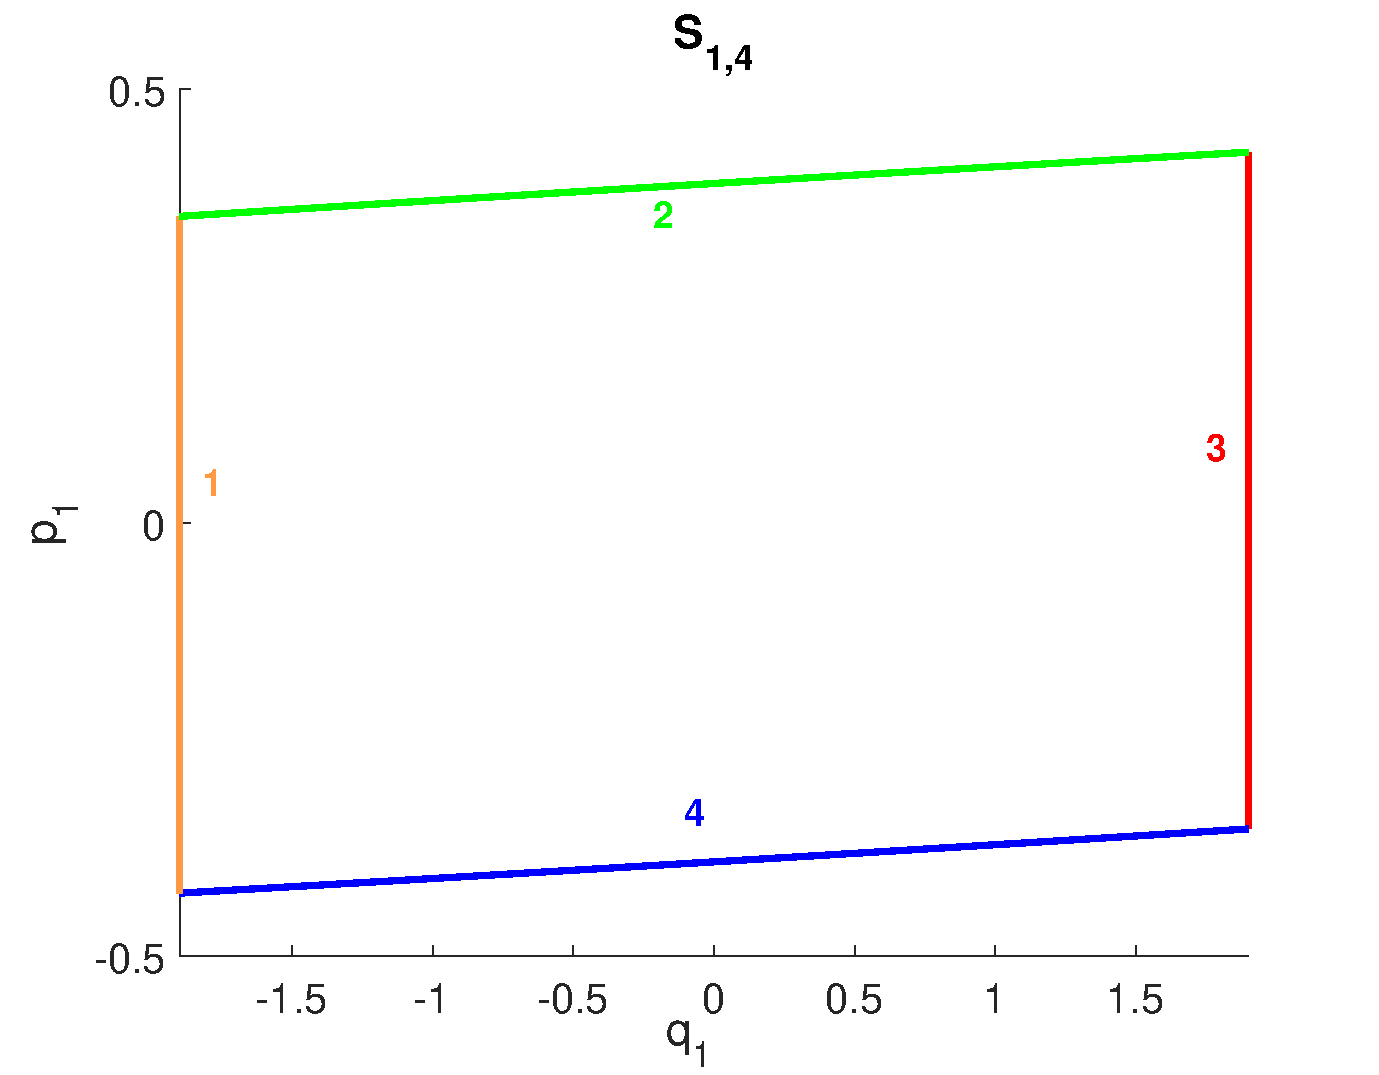
\includegraphics[width=7cm]{S141.pdf}
%   \caption{\footnotesize{Source phase space of line $1$.
%   Boundaries of the region \set{S}{$1$,}{$4$}}.}
%   \label{fig:S14}
% \end{minipage}
% \hspace{2cm}
%  \begin{minipage}[]{.40\textwidth}%[b]{5cm}
%  \centering
%   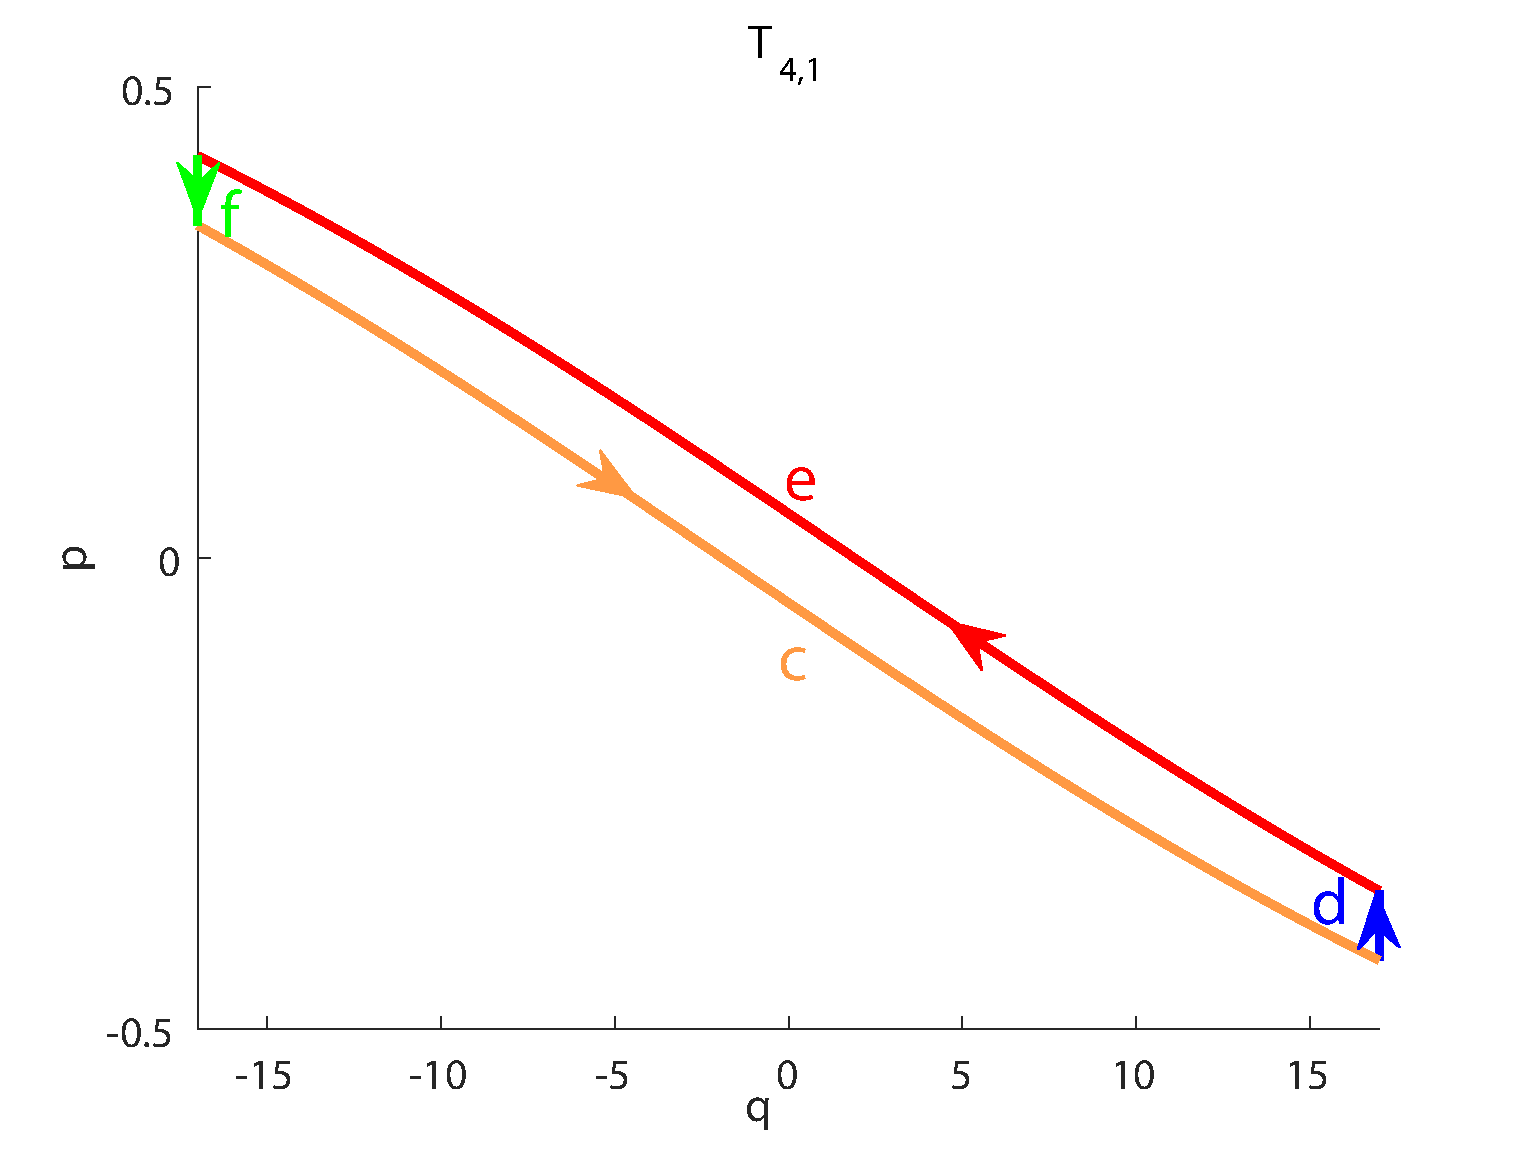
\includegraphics[width=7cm]{T411.pdf}
%   \caption{\footnotesize{Target phase space of line $4$.
%    Boundaries of the region \set{T}{$4$,}{$1$}}.}
%    \label{fig:T411}
% \end{minipage}
% \end{figure}
% Similarly, the boundaries of the lines \setbound{S}{i,}{k}{\variable{j}} and
% \setbound{T}{k,}{i}{\variable{j}} are calculated for every $\variable{j}\in\{2,3,4\}$ and
% the boundaries in Eq. (\ref{eq:analytic_boundaries}) are found. \\
% \begin{figure}
% \begin{minipage}[]{.48\textwidth}% [b]{5cm}
%  % \centering
%   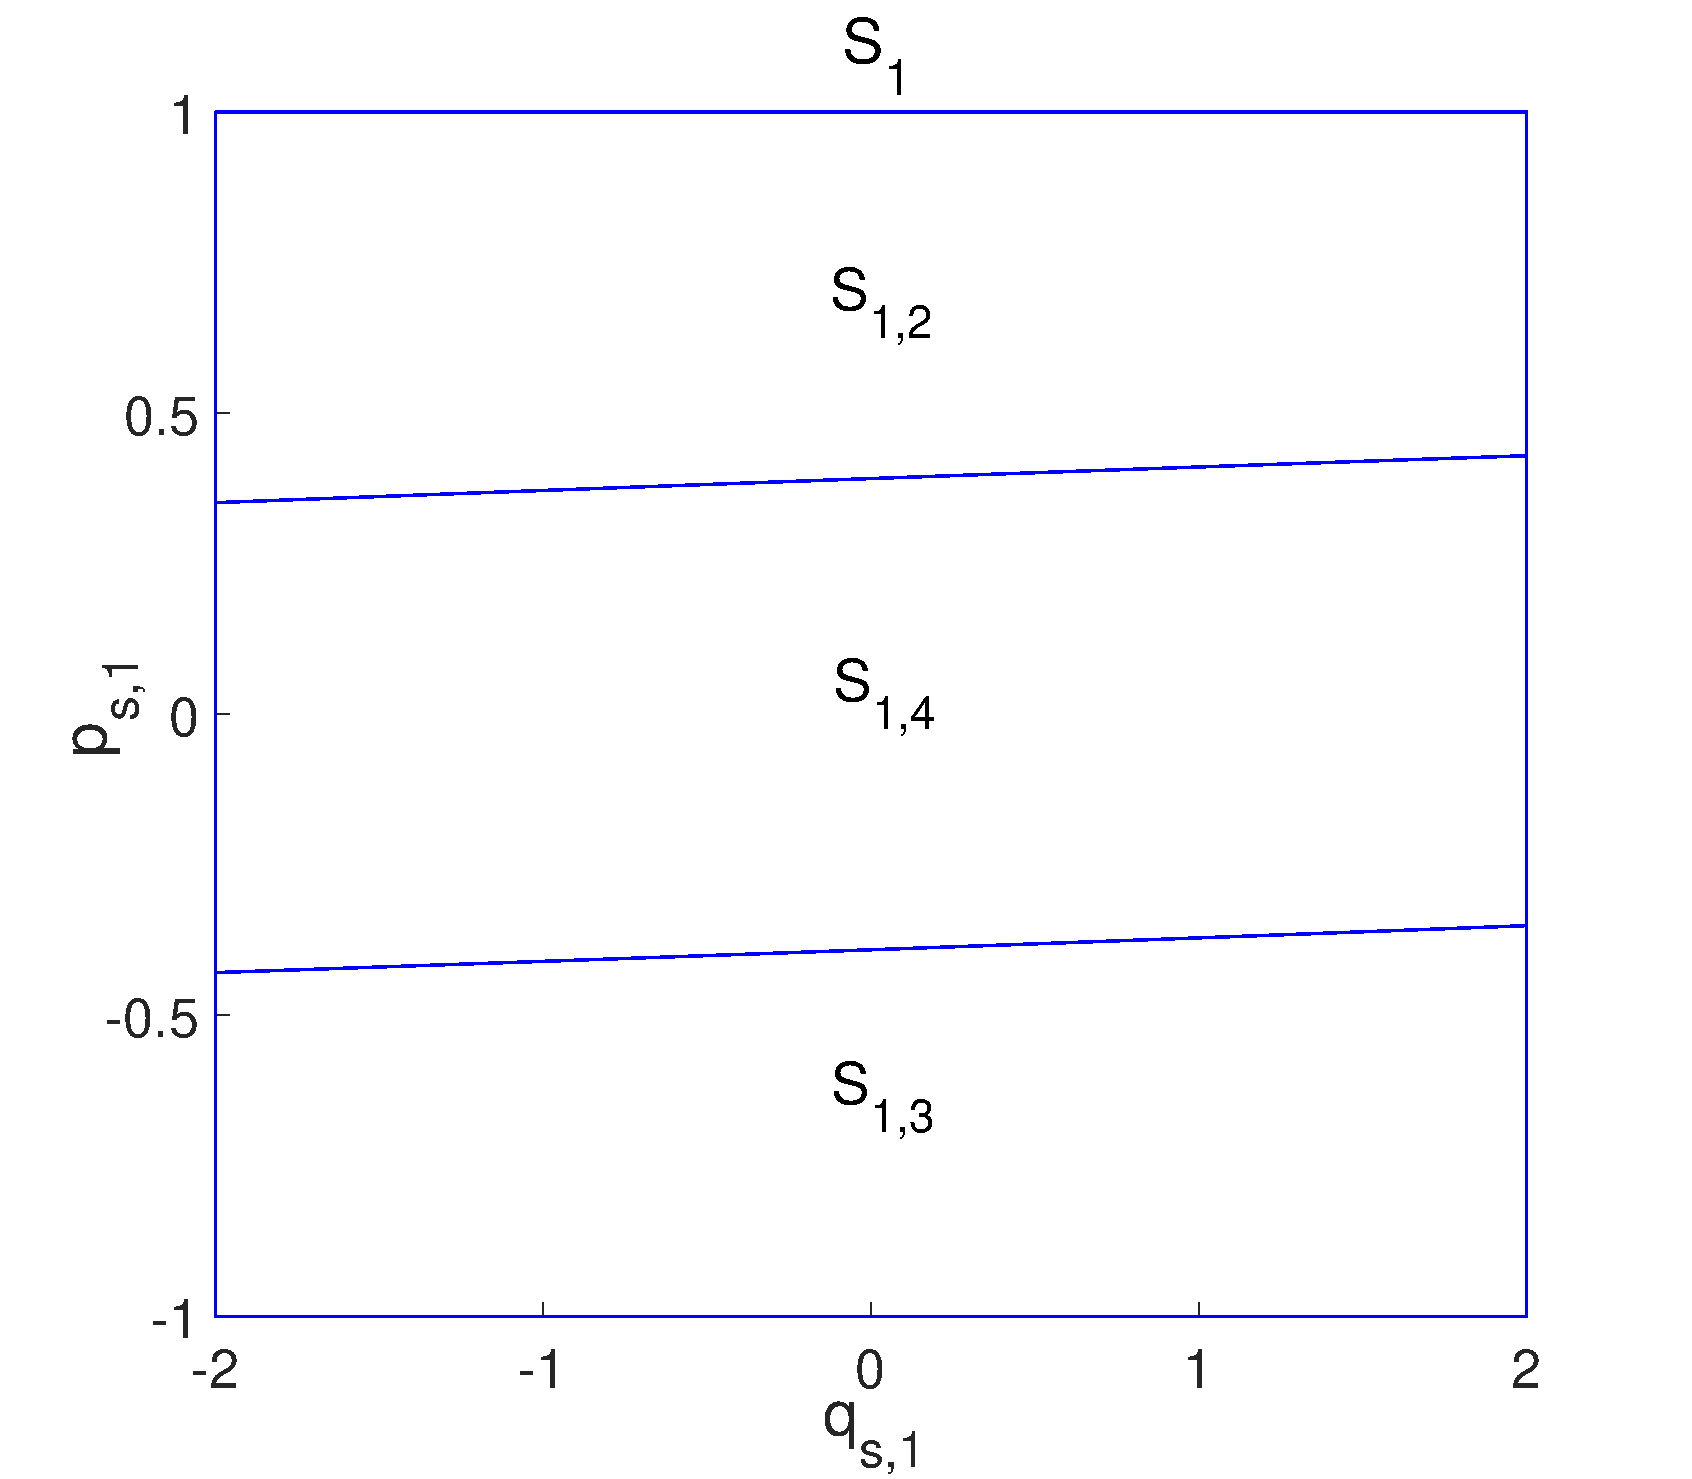
\includegraphics[width=8cm]{S1.pdf}
%\caption{\footnotesize{The PS $\mbox{\set{S}{$1$}{}}$ of line $1$ is partitioned into regions $(\mbox{\set{S}{$1$,}{j}})_{\variable{j} = 2,3,4}$
%   formed by rays that leave line $1$ and hit line $\textit{j}$.}}
%   \label{fig:S1}
% \end{minipage}
%  \begin{minipage}[]{.47\textwidth}% [b]{5cm}
%  \centering
%   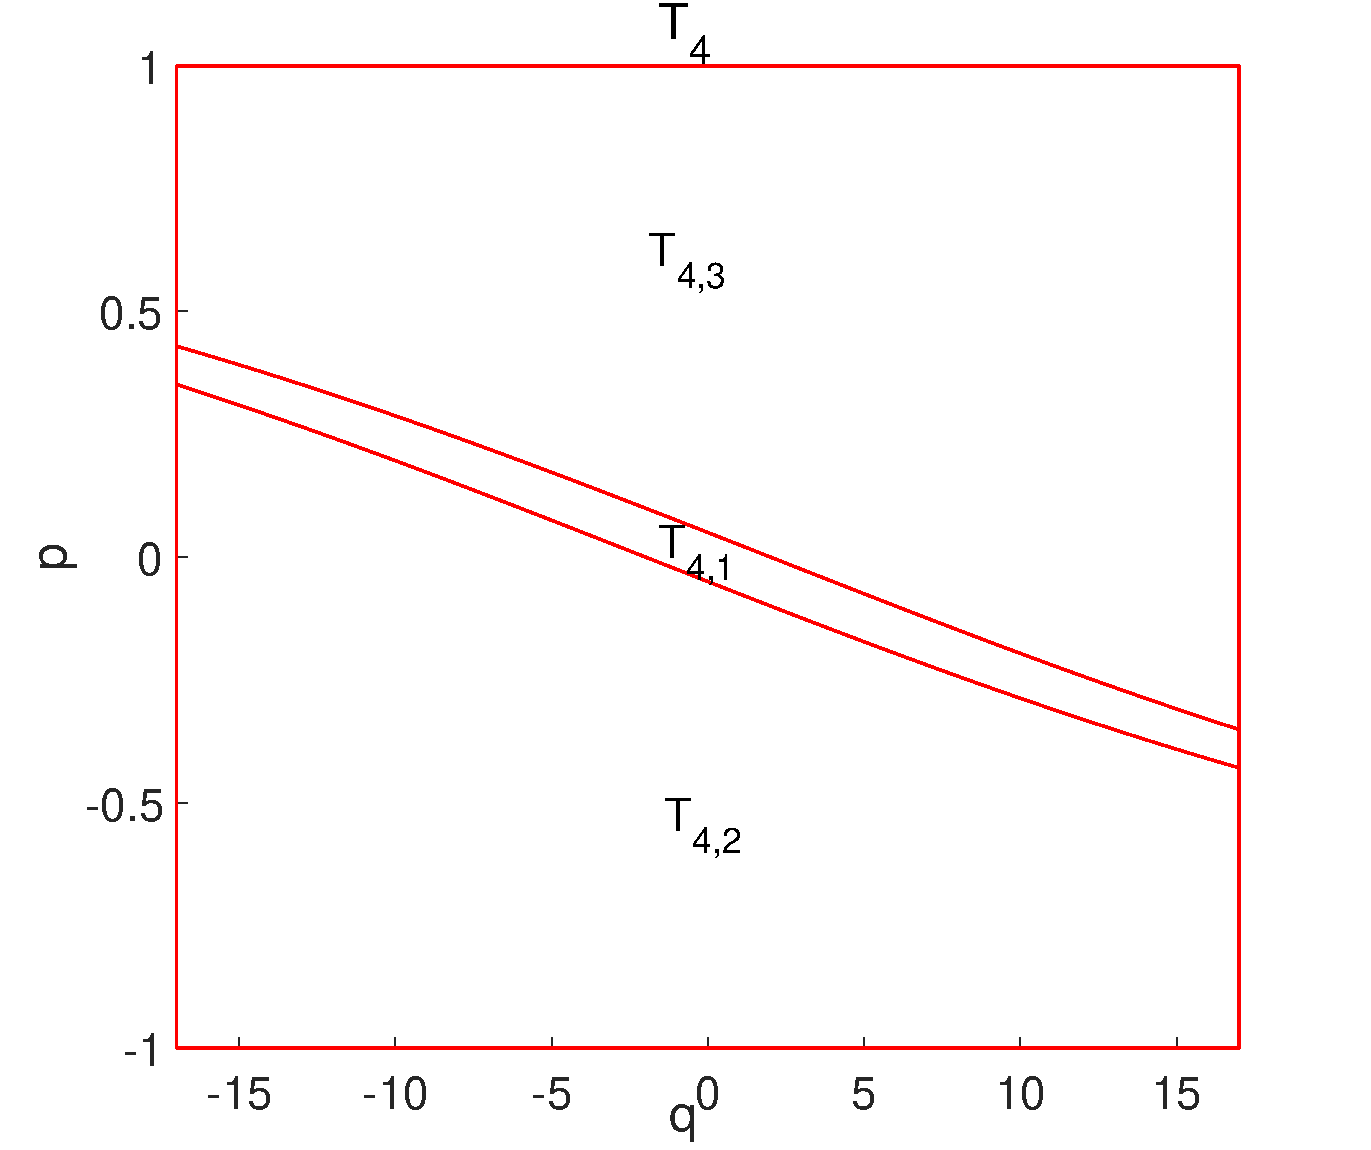
\includegraphics[width=8cm]{T4b.pdf}
%   \caption{\footnotesize{The PS $\mbox{\set{T}{$4$}{}}$ of line $4$ is partitioned into regions $(\mbox{\set{T}{$4$,}{k}})_{\variable{k} = 1,2,3}$
%   formed by rays that leave line $\textit{k}$ and hit line $4$.}}
%   \label{fig:T4b}
% \end{minipage}
%\begin{minipage}[]{.48\textwidth}%[b]{5cm}
%\centering
%   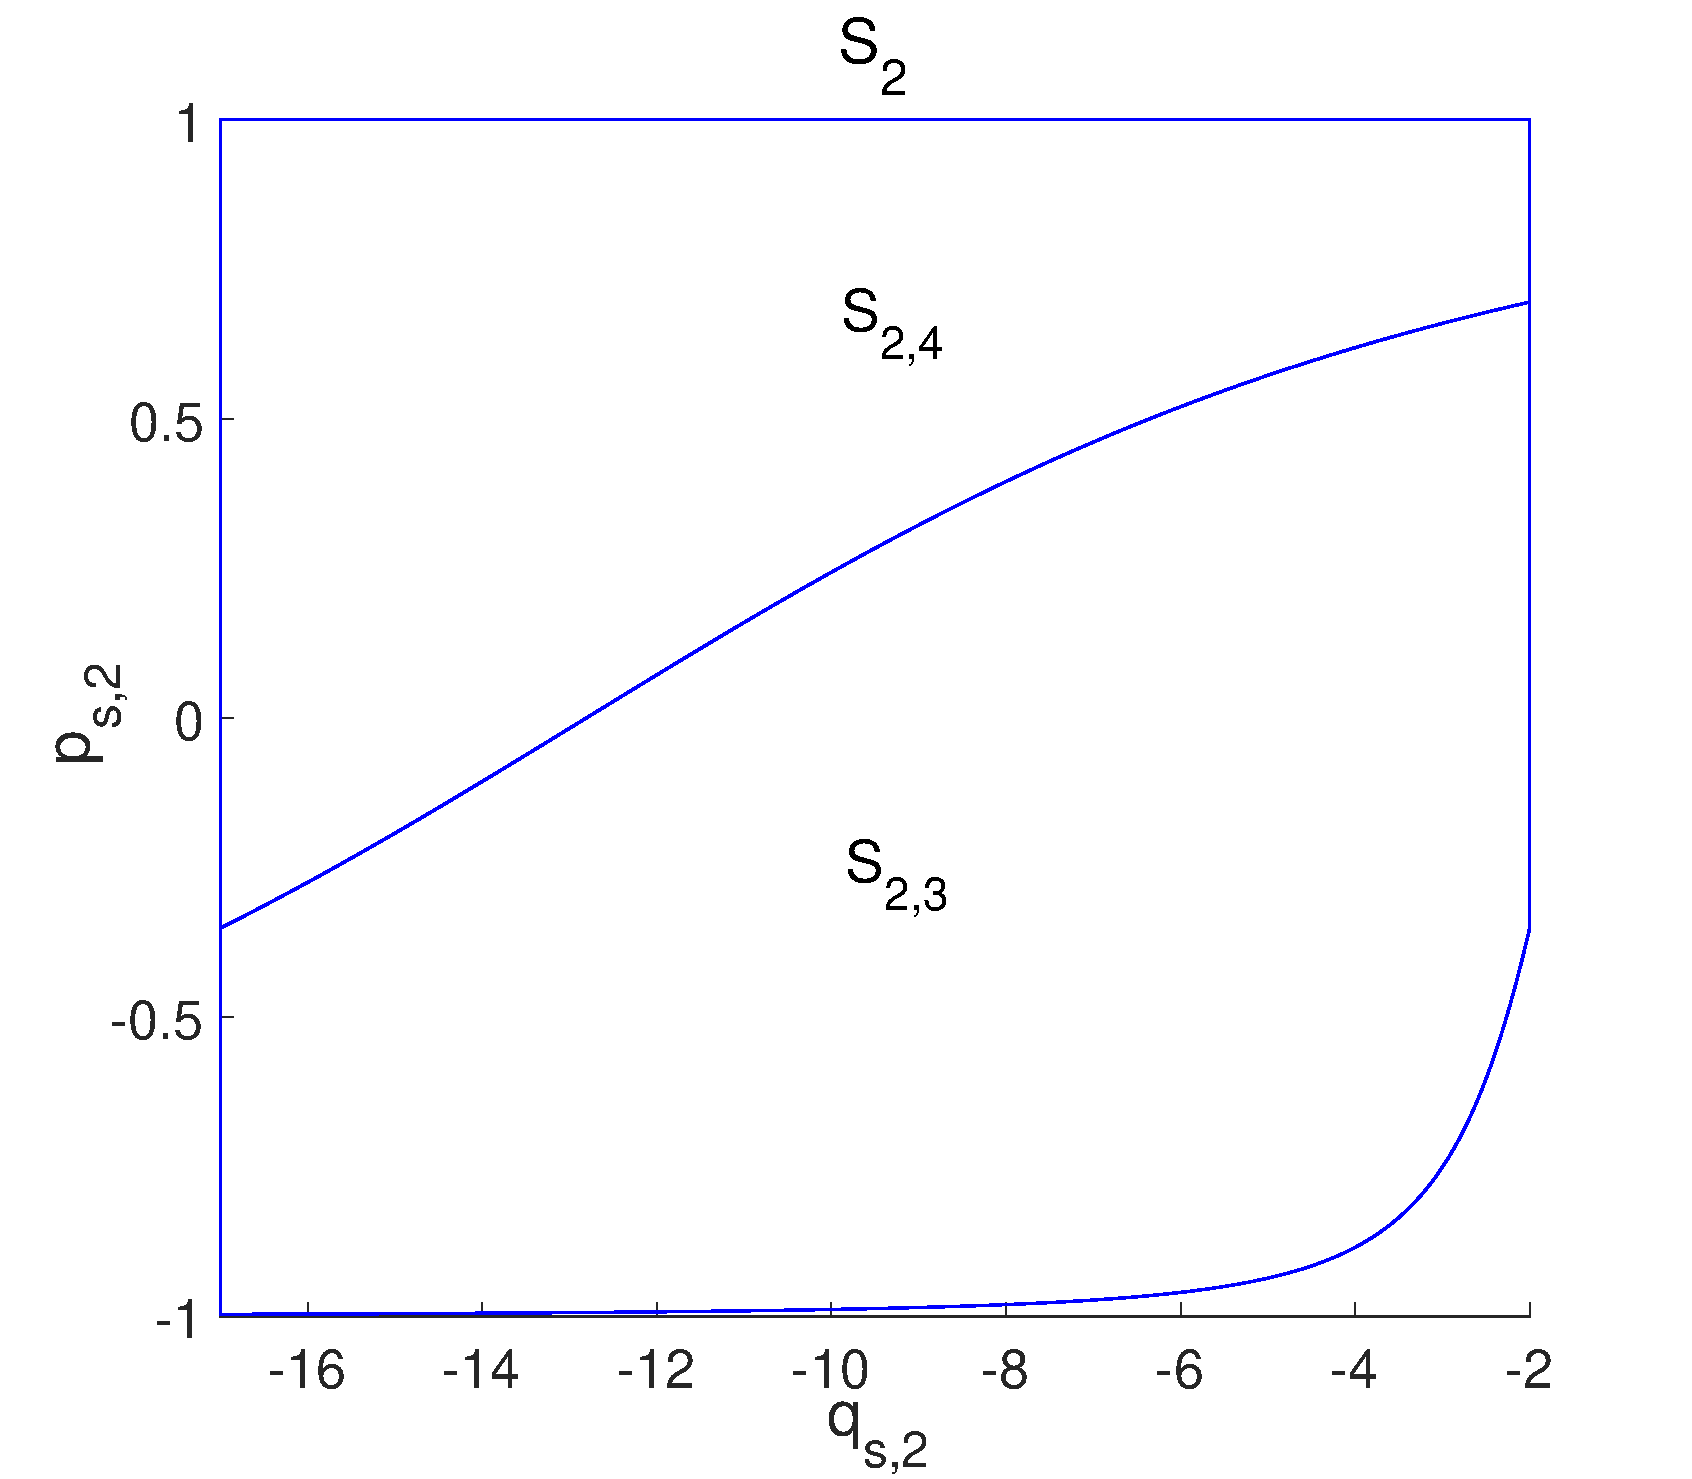
\includegraphics[width=8cm]{S2.pdf}
%\caption{\footnotesize{The PS $\mbox{\set{S}{$2$}{}}$ of line $2$ is partitioned into regions $(\mbox{\set{S}{$2$,}{j}})_{\variable{j} = 3,4}$,
%   formed by rays that leave line $2$ and hit line $\variable{j}$.}}
% \end{minipage}
% \begin{minipage}[]{.47\textwidth}
% \centering
%   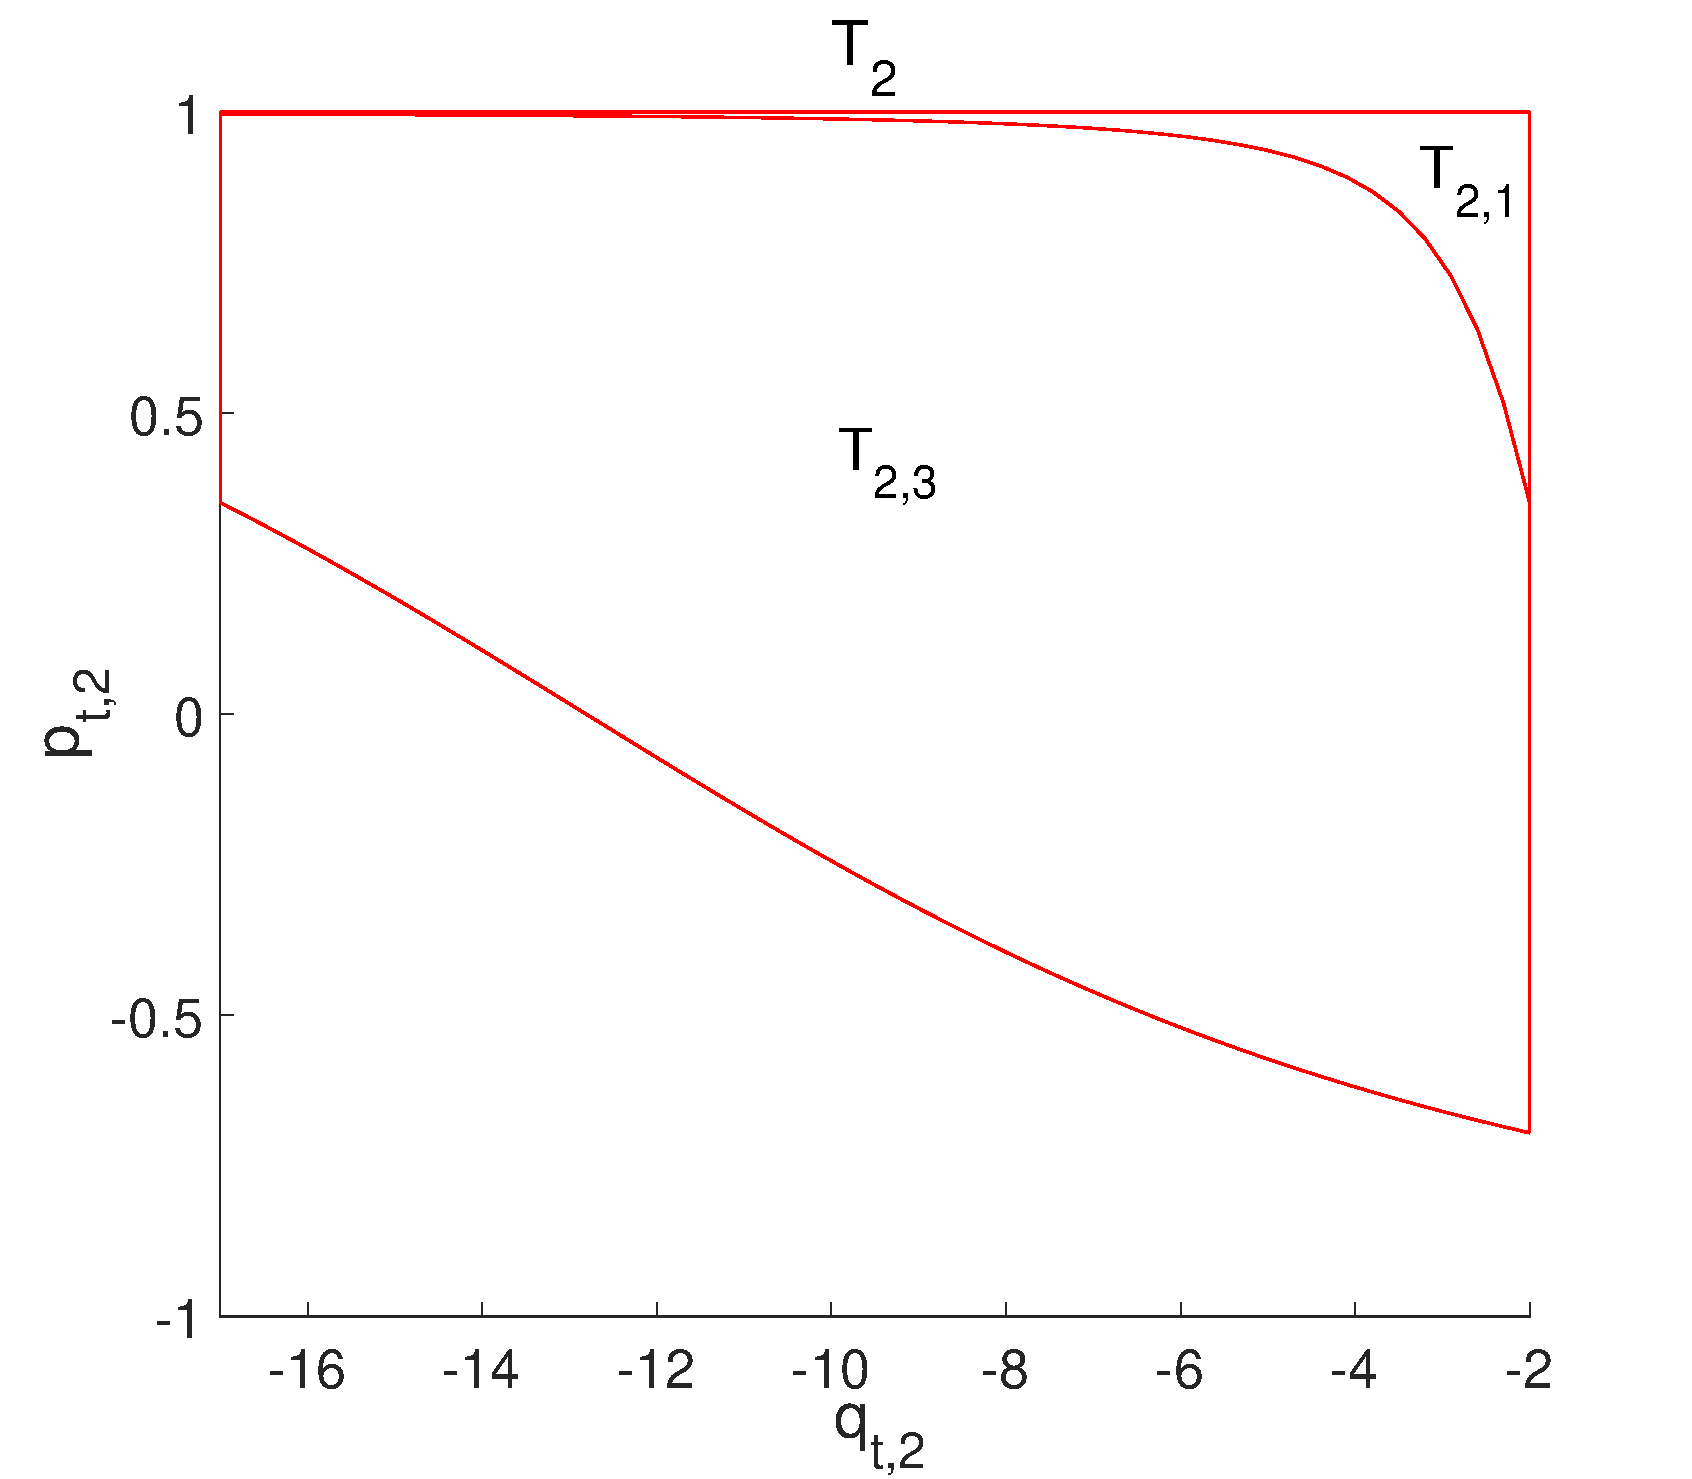
\includegraphics[width=8cm]{T2b.pdf}
%\caption{\footnotesize{The PS $\mbox{\set{T}{$2$}{}}$ of line $2$ is partitioned into regions $(\mbox{\set{T}{$2$,}{k}})_{\variable{k} = 1,3}$
%formed by rays that leave line $\variable{k}$ and hit line $2$.}}
% \end{minipage}
% \begin{minipage}[]{.48\textwidth}
% \centering
%   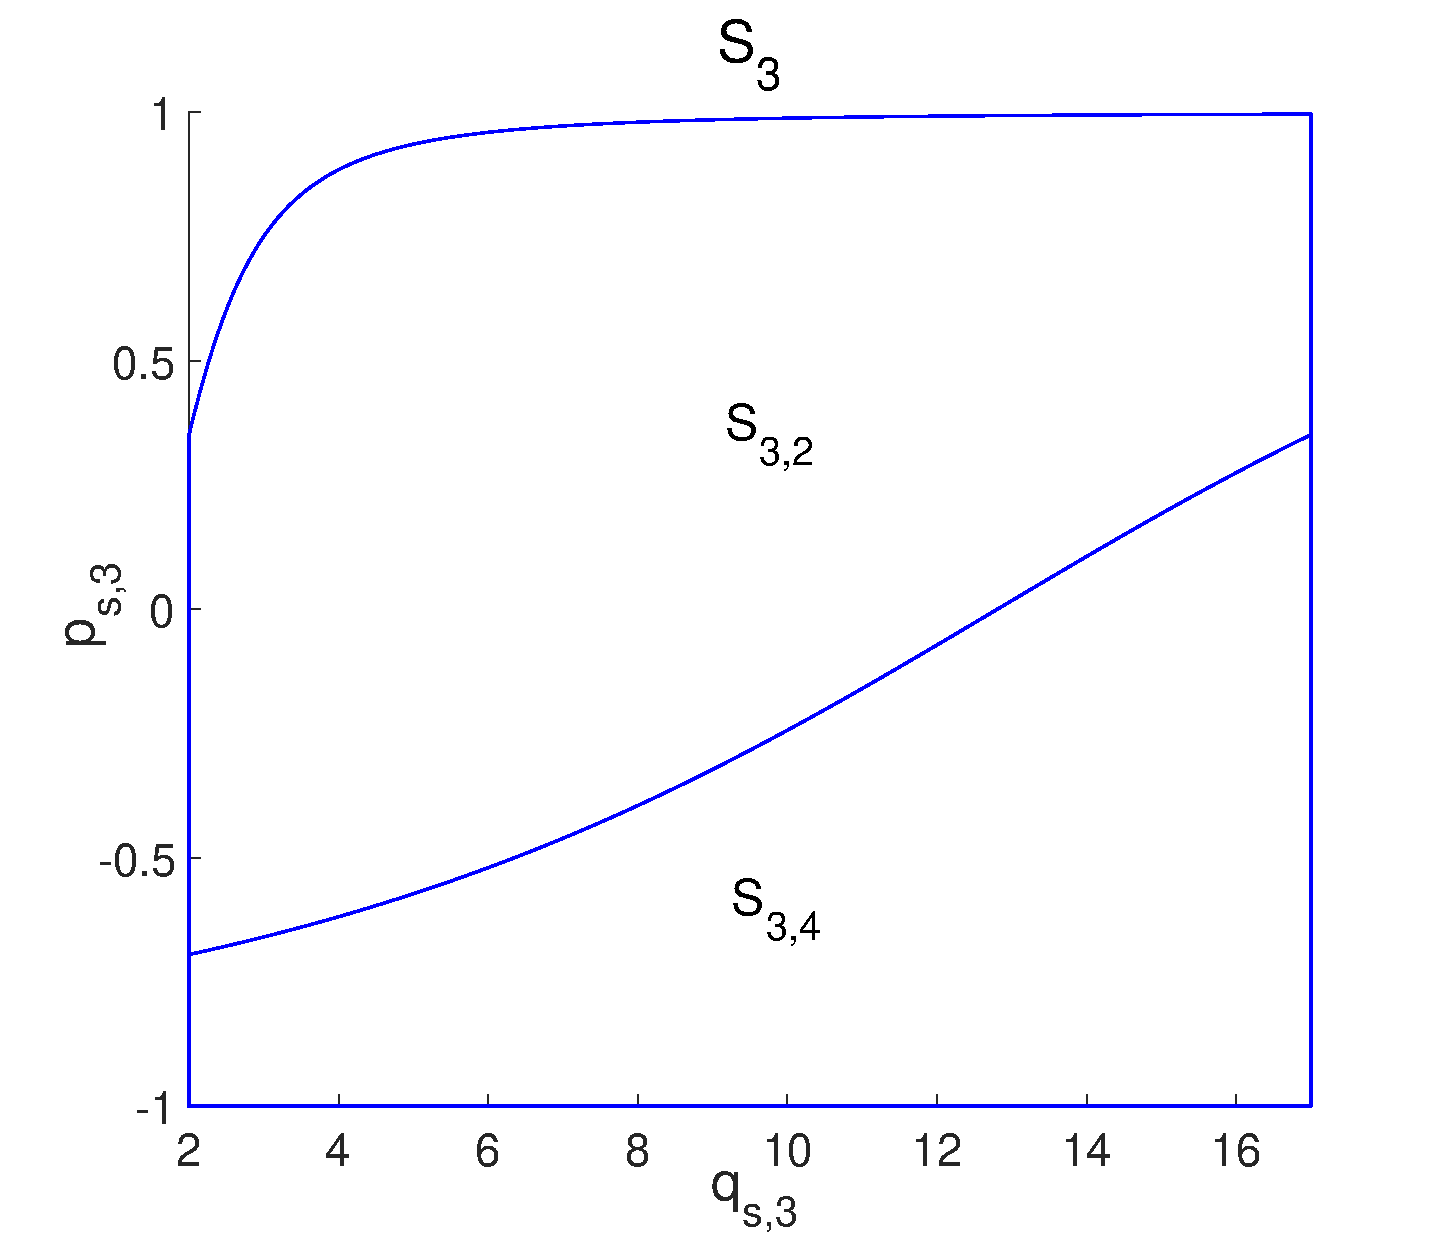
\includegraphics[width=8cm]{S3.pdf}
%   \caption{\footnotesize{The PS $\mbox{\set{S}{$3$}{}}$ of line $3$ is partitioned into regions
%   $(\mbox{\set{S}{$3$,}{j}})_{\variable{j} = 2,4}$ formed by rays that leave line $3$ and hit line $\variable{j}$.}}
% \end{minipage}
% \hspace{0.8cm}
% \begin{minipage}[]{.47\textwidth}
% \centering
%   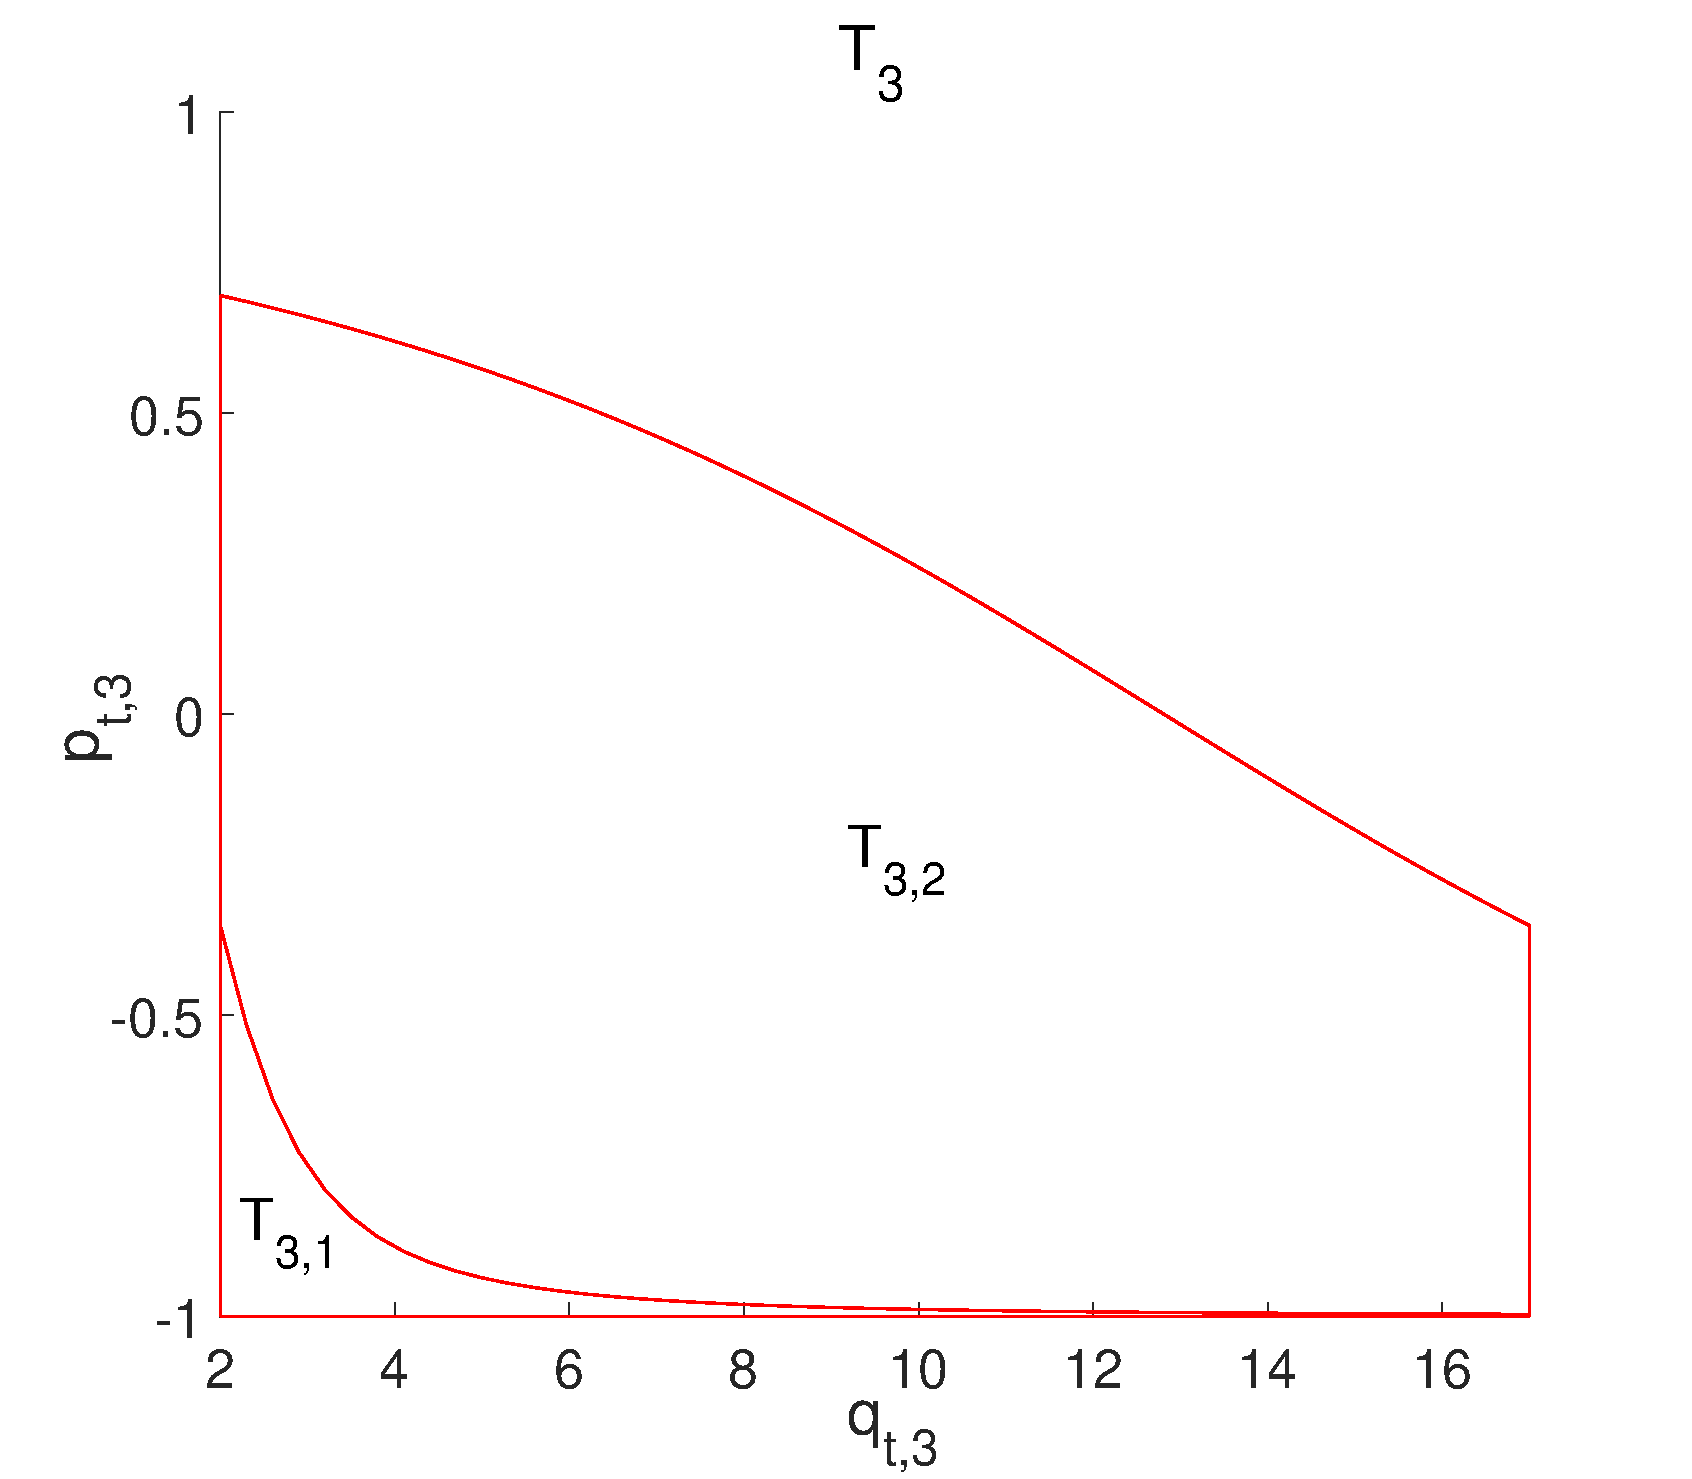
\includegraphics[width=8cm]{T3_b.pdf}
%  \caption{\footnotesize{The PS $\mbox{\set{T}{$3$}{}}$ of line $3$ is partitioned into regions $(\mbox{\set{T}{$3$,}{k}})_{\variable{k} = 1,2}$
%   formed by rays that leave line $\variable{k}$ and hit line $3$.}}
%\label{fig:T3}
% \end{minipage}
%\end{figure}
%\indent In Figs. $\ref{fig:S1}-\ref{fig:T3}$  $(\partial \mbox{\set{S}{i,}{j}})_{\variable{j}=2, 3, 4}$ and $(\partial \mbox{\set{T}{i,}{k}})_{\variable{k}=1, 2, 3}$ are depicted with blue and red lines, respectively. Indeed, those products are the sine of the angle that the ray formes with the normals $\nu_{\variable{i}}$ and $\nu_{\variable{k}}$, respectively.\\
%We observe that, because of the symmetry of the optical system, the \set{S}{$2$}{} and \set{S}{$3$}{} are symmetrical to  each other as well as \set{T}{$2$}{} and \set{T}{$3$}{}, while, due to the reflection law, \set{S}{$2$}{} and \set{T}{$2$}{} are flipped as well as \set{S}{$3$}{} and \set{T}{$3$}{}.
%In the next section, we show how the phase spaces are related to each other and we define the target photometric variables on \set{T}{$4$}{}.
%\subsection{\textbf{Target photometric variables}}
%In this section we explain how to compute the target photometric variables in PS.
%In the following, to simplify the notation, we indicate the target coordinates of the rays on \set{T}{$4$}{} with (\variable{q}, \variable{p}) instead of $(\pos{t,}{$4$}, \dir{t,}{$4$})$.
%The intensity $I$ along a given direction $\variable{p}\in [-1,1]$ in target phase space \set{T}{$4$}{} is defined as a function of the output luminance $L(\variable{q}, \variable{p})$:
%\begin{equation}\label{I(eta)}
%I_{PS}(\variable{p}) = \int_{-\variable{b}}^{\variable{b}} L(\variable{q},\variable{p}) \textrm{d}\variable{q}\,.
%\end{equation}
%Note that the intensity is a function of $\variable{p}= \sin(\theta)$ instead of $\theta$.
%The parts of \set{T}{$4$}{} that are illuminated by \set{S}{$1$}{} correspond to parts with positive luminance, for the other parts the luminance is equal to zero.
%Assuming positive luminance on \point{S}, the following relations hold:
%\begin{subequations}\label{LT4}
%\begin{align}
%L(\variable{q}, \variable{p})&>0 \qquad \quad \forall (\variable{q}, \variable{p})\in \mbox{\set{T}{$4$,}{$1$}},\\
%L(\variable{q}, \variable{p})&\geq 0 \qquad\quad \forall(\variable{q}, \variable{p}) \in (\mbox{\set{T}{$4$,}{i}})_{\variable{i}=2,3}.\label{third}
%\end{align}
%\end{subequations}
%Once a ray leaves the source \point{S} it can hit the reflectors several times before hitting the target \point{T}. To relate \point{S} and \point{T}, a map \map{M}{$1$,}{$4$}:\set{S}{$1$}{}$\rightarrow$ \set{T}{$4$}{} is introduced such that $\mbox{\map{M}{$1$,}{$4$}}(\pos{s,}{$1$},\dir{s,}{$1$})=(\variable{q},\variable{p})$.
%As  not all the parts of \set{T}{$4$}{} are illuminated by the source \point{S}, the map
%\map{M}{$1$,}{$4$} is not surjective.
%Therefore, we need to determine the subsets of \set{T}{$4$}{} illuminated by \point{S} corresponding to the regions where the luminance is positive.
%To this purpose, we consider two different kind of maps.
%The first map relates the coordinates of the source and the target PS of two \textit{different} lines, we call this map the propagation map.
%The second map relates the coordinates of the target and the source PS of the \textit{same} line, we call it the reflection map.
%In particular, given two lines \variable{i} and \variable{j} with \variable{i}$\neq$\variable{j}, the propagation map \map{P}{i,}{j}:\set{S}{i,}{j}$\mapsto$\set{T}{j,}{i} relates the regions \set{S}{i,}{j} with the regions \set{T}{j,}{i}.
%For one single line \variable{j}, the reflection map \map{R}{j}{}: \set{T}{j}{} $\mapsto$\set{S}{j}{} relates the regions \set{T}{j}{} and
%\set{S}{j,}{}. \map{P}{i,}{j} is defined as follows:
% \begin{equation}\label{Pij}
%\mbox{\map{P}{i,}{j}}(\pos{s,}{i},\dir{s,}{i})=(\pos{t,}{j},\dir{t,}{j}),
%\end{equation}
%where $\pos{t,}{j}$ is given by the \variable{x}-coordinate of the intersection point between the ray and line \variable{j},
%while $\dir{t,}{j}$ is computed considering the direction of the reflected ray with respect to the normal of line \variable{j}. \map{R}{j}{} is defined as follows:
%\begin{equation}\label{Rj}
%\mbox{\map{R}{j}{}}(\variable{q}_{\textrm{t},\textit{j}},\variable{p}_{\textrm{t},\textit{j}})=(\variable{q}_{\textrm{s},\textit{j}},\variable{p}_{\textrm{s},\textit{j}}),
%\end{equation}
% where the direction $\dir{t,}{j}$ changes according to the reflection law and the position $\pos{t,}{j}= \pos{s,}{j}$ as it maps the target PS into the source PS of the same line \variable{j}.
%Using a procedure similar to the ray transport matrices approach (see \cite{Hecht}, Chapter 6),
%the map \map{M}{$1$,}{$4$} is described by the composition of mappings \map{P}{i,}{j} and \map{R}{j}{} defined in Eqs.
%$(\ref{Pij})$ and $(\ref{Rj})$, respectively. This composition depends on the path $\Pi$ followed by the rays where we refer to a path as the sequence of lines that
% a ray hits during its propagation from \point{S} to \point{T}. We indicate with \map{M}{$1$,}{$4$}($\Pi$)
%the map \map{M}{$1$,}{$4$} restricted to path $\Pi$ and with $\mbox{\set{R}{}{}}(\Pi)\subset \mbox{\set{T}{$4$}{}}$ the regions on \set{T}{$4$}{} formed by the rays that follow path $\Pi$.
%Considering all the possible paths $\Pi$ from \point{S} to \point{T}, all the regions $\mbox{\set{R}{}{}}(\Pi)$ with positive luminance on \set{T}{$4$}{} can be determined.
%\\ \indent To clarify this concept, we provide the following example.
%Consider a ray that is emitted from the source (line $1$), hits first the left reflector (line $2$) and finally reaches the target (line $4$).
% The path $\Pi$ followed by this ray is defined as $\Pi =(1, 2, 4)$ and
% the corresponding map $\mbox{\map{M}{$1$,}{$4$}}(\Pi):\mbox{\set{S}{$1$}{}}\mapsto \mbox{\set{R}{}{}}(\Pi)$ that describes the propagation of all rays that follow the path $\Pi$ is defined by:
%\begin{equation}
%\label{map_example}
%\mbox{\map{M}{$1$,}{$4$}}(\Pi):\mbox{\set{S}{$1$,}{$2$}}\mapsto \mbox{\set{T}{$2$,}{$1$}}\mapsto\mbox{\set{S}{$2$,}{$4$}}\mapsto \mbox{\set{T}{$4$,}{$2$}}\,.
%\end{equation} Using the notation introduced above, we can write the previous relation as:
%\begin{equation}
%\mbox{\map{M}{$1$,}{$4$}}({\Pi}) = \mbox{\map{P}{$2$,}{$4$}}
%\circ \mbox{\map{R}{$2$}{}}\circ \mbox{\map{P}{$1$,}{$2$}}\,.
%\end{equation}
%Therefore, to construct the maps $\mbox{\map{M}{$1$,}{$4$}}(\Pi)$ we need to know its corresponding path $\Pi$.
%To determine all the possible paths $\Pi$,
%instead of tracing the rays from \point{S} to \point{T}, we start considering the rays in \set{T}{$4$}{}.
%In particular, along a given direction $\variable{p}\in[-1,1]$ we consider the intersection points between the line $\variable{p}=\mbox{const}$ and $(\partial\mbox{\set{T}{$4$,}{i}})_{\variable{i}\in\{1, 2, 3\}}$. These points are traced back to the line \variable{i} from which they are emitted and their corresponding coordinates on \set{S}{i}{} and \set{T}{i}{} are computed. This is done applying sequentially the maps $\mbox{\inversemap{P}{i,}{$4$}}:\mbox{\set{T}{$4$,}{i}}\mapsto\mbox{\set{S}{i,}{$4$}}$ and $\mbox{\inversemap{R}{i}{}}:\mbox{\set{S}{i}{}}\mapsto\mbox{\set{T}{i}{}}$.
%Then the same procedure is repeated considering these new coordinates on \set{T}{i}{}.
%The computation stops either when the points found are emitted from the source, that is when they are located on \set{S}{$1$}{}, or when they reach again the target, that is when they are located on \set{T}{$4$}{}.
%If the ray reaches \set{S}{$1$}{}, then a path $\Pi$ from \point{S} to \point{T} is found.
%If the ray reaches again the target \set{T}{$4$}, then we conclude that it is not emitted by
%\point{S} and therefore, it is located inside the parts of \set{T}{$4$}{} with luminance equal to zero. \\ \indent
% Finally, the inverse $\mbox{\inversemap{M}{$1$,}{$4$}}(\Pi)$ of the map \map{M}{$1$,}{$4$}$(\Pi)$ is constructed for every possible path $\Pi$.
% The map \inversemap{M}{$1$,}{$4$}$(\Pi)$ is the composition of the inverse of the propagation and the reflection maps in reverse order according to path $\Pi$.
%For instance, for path $\Pi = (1,2,4)$, \inversemap{M}{$1$,}{$4$}$(\Pi)$ is given by:
%\begin{equation}
%\label{inverse_map}
%\mbox{\inversemap{M}{$1$,}{$4$}}({\Pi}) = \mbox{\inversemap{P}{$1$,}{$2$}}
%\circ \mbox{\inversemap{R}{$2$}{}}\circ \mbox{\inversemap{P}{$2$,}{$4$}}.
%\end{equation}
%The steps of the procedure are shown in the graph in Fig. \ref{fig:tree} where the map in Eq. (\ref{inverse_map}) is written in red. \\
%\begin{figure}
%\centering
%\begin{tikzpicture}
%  [
%    grow                    = down,
%    sibling distance        = 9em,
%    level distance          = 7em,
%    edge from parent/.style = {draw, -latex},
%    selected edge from parent/.style = {draw, -latex},
%    every node/.style       = {font=\footnotesize},
%    sloped
%  ]
%  \node [root] {$\mbox{\set{T}{$4$}{}}$}
%   child { node [env] {$\mbox{\set{S}{$2$,}{$4$}}$}
%   child { node [root] {\set{T}{$2$}{}}
%   %\draw[dashed,bend right](0-1)to(0-3);
%    child { node [env] {\set{S}{$1$,}{$2$}}
%          edge from parent node [above] {\textcolor{red}{$\mathrm{P}_{1,2}^{-1}$} }}
%        child { node [env] {\set{S}{$3$,}{$2$}}
%         child { node [root] {\set{T}{$3$}{}}
%         child { node [env] {\set{S}{$1$,}{$3$}}
%             edge from parent node [above] {$\mathrm{P}_{1,3}^{-1}$}
%             }
%             child { node [env] {\set{S}{$2$,}{$3$}}
%             edge from parent node [above] {$\mathrm{P}_{2,3}^{-1}$}
%             }
%         edge from parent node [above] {$\mathrm{R}_{3}^{-1}$}
%         }
%          edge from parent node [above] {$\mathrm{P}_{3,2}^{-1}$}
%                            }
%        edge from parent node [above] {\textcolor{red}{$\mathrm{R}_{2}^{-1}$}}
%   }
%   edge from parent node [above] {\textcolor{red}{$\mathrm{P}_{2,4}^{-1}$}}
%   }
%    child { node [env] {\set{S}{$1$,}{$4$}}
%      edge from parent node [above] {$\mathrm{P}_{1,4}^{-1}$}
%      }
%    child { node [env] {\set{S}{$3$,}{$4$}}
%      child { node [root] {\set{T}{$3$}{}}
%        child { node [env] {\set{S}{$1$,}{$3$}}
%       edge from parent node [above] {$\mathrm{P}_{1,3}^{-1}$} }
%        child { node [env] {\set{S}{$2$,}{$3$}}
%         child { node [root] {\set{T}{$2$}{}}
%         child { node [env] {\set{S}{$1$,}{$2$}}
%             edge from parent node [above] {$\mathrm{P}_{1,2}^{-1}$}
%             }
%             child { node [env] {\set{S}{$3$,}{$2$}}
%             edge from parent node [above] {$\mathrm{P}_{3,2}^{-1}$}
%             }
%         edge from parent node [above] {$\mathrm{R}_{2}^{-1}$}
%         }
%          edge from parent node [above] {$\mathrm{P}_{2,3}^{-1}$}
%                           }
%            edge from parent node [above] {$\mathrm{R}_{3}^{-1}$}
%                            }
%            edge from parent node [above] {$\mathrm{P}_{3,4}^{-1}$}
%            };
%        %    \tikzset{every tree node/.style={align=center,anchor=north}}
%
%
%\end{tikzpicture}
%\\
%\caption{Tree that describes how to detect all the possible paths from \point{S} to \point{T}.}
%\label{fig:tree}
%\end{figure}
%\newpage
%\indent Using the procedure explained above, given a ray with coordinates
%$(\variable{q}, \variable{p})\in \mbox{\set{T}{$4$}{}}$ we can establish whether it is located inside one of the regions $\mbox{\set{R}{}{}}(\Pi)$ with positive luminance or not.
%In case the ray is inside a region $\mbox{\set{R}{}{}}(\Pi)$,
%its corresponding coordinates $(\pos{s,}{$1$},\dir{s,}{$1$})\in \mbox{\set{S}{$1$}{}}$ are obtained using $\mbox{\inversemap{M}{$1$,}{$4$}}(\Pi)$, where $\Pi$ is the path followed by this ray. Eq. ($\ref{LT4}$) becomes:
%\begin{subequations}\label{LT}
%\begin{align}
%L(\variable{q}, \variable{p})&>0 \qquad \quad \forall (\variable{q}, \variable{p})\in \mbox{\set{R}{}{}}(\Pi),\\
%L(\variable{q}, \variable{p})&= 0 \qquad \quad \mbox{otherwise},\label{third}
%\end{align}
%\end{subequations}
%for some path $\Pi$ connecting \point{S}{}{} and \point{T}{}{}.
%Assuming a Lambertian source and employing conservation of luminance along a ray (see \cite{Chaves}, Chapter 16), we have that $L$
%is a positive constant inside \set{R}{}{}($\Pi$) and it is equal to zero on the other parts of \set{T}{$4$}{}.
%Indicating with $\variable{q}^\textrm{\,min}(\Pi,\variable{p})$ and $\variable{q}^\textrm{\,max}(\Pi,\variable{p})$ the minimum and maximum position coordinates of the intersection points between the boundaries $ \partial$\set{R}{}{}($\Pi$) and line $\variable{p}= \mbox{const}$,
%Eq. (\ref{I(eta)}) reduces to:
%\begin{equation}\label{eta2}
%I_{PS}(\variable{p}) = \sum_{\Pi}\int_{\variable{q}^\textrm{\,min}(\Pi, \variable{p})}^{\variable{q}^\textrm{\,max}(\Pi,\variable{p})}L(\variable{q}, \variable{p})\textrm{d}\variable{q} =
%\sum_{\Pi}\big (\variable{q}^\textrm{max}(\Pi,\variable{p})-\variable{q}^\textrm{\,min}(\Pi,\variable{p})\big )\,,
%\end{equation}
%where the sum is over all the possible paths and the second equation holds as we assume $L=1$ in \set{R}{}{}($\Pi$).
%In the next paragraph the details of the procedure to compute the coordinates $\variable{q}^\textrm{\,min}(\Pi, \variable{p})$ and $\variable{q}^\textrm{\,max}(\Pi, \variable{p})$
%are explained.
%\subsection{\textbf{The structure of the algorithm}}\label{algorithm}
%The goal is to determine the intensity of the light that reaches the target in a given direction $\variable{p}=\mbox{const}$.
%Since we assume a Lambertian source, this is given by the sum of the width of the intervals formed by rays
%emitted in direction $\variable{p} = \mbox{const}$, where every interval is formed by the rays that follow the same path (see Eq. (\ref{eta2})).
%To determine these intervals, a recursive procedure is developed.
%The procedure starts considering on \set{T}{$4$}{} the two parallel rays that hit the extremes 
%of the target with direction $\variable{p}$. 
%These rays are traced back from \set{T}{$4$}{} to \set{T}{i}{} where \variable{i} is the line from which
%the traced rays are emitted. Then, another interval of parallel rays along the corresponding direction of $\variable{p} = \mbox{const}$ on \set{T}{i}{} has to be considered on \set{T}{i}{}.
%The rays corresponding
%to the points located at the extremes of this interval are traced back from $\variable{i}$ to the line from which the are emitted.
%The procedure continues recursively until the source is found.
%This allows to determine
%all the possible paths that can occur for the rays that reach the target at direction $\variable{p}$.
%Furthermore, using our method, the coordinates of the points located at the extremes of the interval formed by all the rays that follow the same path and reach the
%target at direction $\variable{p} = \mbox{const}$ can be determined.
%\\ \indent Before explaining how this can be done, let us introduce some notations.
%The coordinates on \set{T}{j}{} of points traced back from line $\variable{i}\neq\variable{j}$ to
%line $\variable{j}$ are indicated with $(\pos{t,}{j}^\textrm{\,min}, \dir{t,}{j})$ and $(\pos{t,}{j}^\textrm{\,max}, \dir{t,}{j})$ where $\pos{t,}{j}^\textrm{\,min}<\pos{t,}{j}^\textrm{\,max}$. For $\variable{j}=4$ we omit the index $\variable{j}$, so these coordinates on \set{T}{$4$}{} are indicated with
%$(\variable{q}^\textrm{\,min}, \variable{p})$ and $(\variable{q}^\textrm{\,max}, \variable{p})$ where $\variable{q}^\textrm{\,min}<\variable{q}^\textrm{\,max}$.
%The intersection points of line
%$\variable{p}= \dir{t,}{j}$ with boundaries $\partial$\set{T}{j,}{i} need to be determined for every $\variable{i} = \{1,2,3\}$ and $\variable{j} = \{2,3,4\}$ with $\variable{j}\neq\variable{i}$.
%For $\variable{j}\neq 4$, the coordinates of these intersections are indicated with $(\variable{u}_{\variable{j},\variable{i}}^\textrm{\,min}, \dir{t,}{j})$ and $(\variable{u}_{\variable{j},\variable{i}}^\textrm{\,max}, \dir{t,}{j})$ points where $\variable{u}_{\variable{j},\variable{i}}^\textrm{\,min}<\variable{u}_{\variable{j},\variable{i}}^\textrm{\,max}$.
%For $\variable{j} = 4$,
%the coordinates of the intersection points of line $\variable{p}= const$ with $\partial$\set{T}{$4$,}{i} are indicated with $(\variable{u}_{\variable{i}}^\textrm{\,min}, \variable{p})$ and $(\variable{u}_{\variable{i}}^\textrm{\,max}, \variable{p})$ for every $\variable{i}=1,2,3$.
%Since not all the rays whose corresponding coordinates are located inside the interval
%$[(\pos{t,}{j}^\textrm{\,min}, \dir{t,}{j}), (\pos{t,}{j}^\textrm{\,max}, \dir{t,}{j})]$ follow the same path,
% the intersection segment between the two intervals $[(\pos{t,}{j}^\textrm{\,min},\dir{t,}{j}),(\pos{t,}{j}^\textrm{\,max}, \dir{t,}{j})]$ and
%$[(\variable{u}_{\variable{j}, \variable{i}}^\textrm{\,min},\dir{t,}{j}) (\variable{u}_{\variable{j}, \variable{i}}^\textrm{\,max}, \dir{t,}{j})]$ need to be considered on \set{T}{j}{}.
%The coordinates of the extremes of the intersection interval
%are indicated with $(\variable{v}_{\variable{j}, \variable{i}}^\textrm{\,min},\dir{t,}{j})$ and $(\variable{v}_{\variable{j}, \variable{i}}^\textrm{\,max},\dir{t,}{j})$ where
%$\variable{v}_{\variable{j}, \variable{i}}^\textrm{\,min} = \max\{\pos{t,}{j}^ \textrm{\,min},\variable{u}_{\variable{j}, \variable{i}}^\textrm{\,min}\}$ and
% $\variable{v}_{\variable{j}, \variable{i}}^\textrm{\,max} = \min\{\pos{t,}{j}^ \textrm{\,max},\variable{u}_{\variable{j}, \variable{i}}^\textrm{\,max}\}$ when $\variable{j}\neq 4$ and with 
% $\variable{v}_{\variable{i}}^\textrm{\,min} = \max\{\pos{}{}^ \textrm{\,min},\variable{u}_{\variable{i}}^\textrm{\,min}\}$ and
% $\variable{v}_{\variable{i}}^\textrm{\,max} = \min\{\pos{}{}^ \textrm{\,max},\variable{u}_{\variable{i}}^\textrm{\,max}\}$ when $\variable{j} = 4$. \\ \indent
%To explain the technique, we make use of an example that describes how the target intensity along direction $\variable{p}= -0.2$ is calculated.
%From Fig. $\ref{fig:T41}$ to Fig. $\ref{fig:T43}$ the steps used in this example are shown.
%A detailed description of those figures is given in the following.
%\\ \indent The procedure starts considering the rays with coordinates $(\variable{q}^\textrm{min}, \variable{p})$ and $(\variable{q}^\textrm{max}, \variable{p})$ on \set{T}{$4$}{}, where $\variable{q}^\textrm{min}= -\variable{b}$ and
%$\variable{q}^\textrm{max}= \variable{b}$ are the left and the right extreme of the target \point{T}, respectively.
% The intersection points $(\variable{u}_{\variable{i}}^\textrm{\,min}, \variable{p})$ and
%$(\variable{u}_{\variable{i}}^\textrm{\,max}, \variable{p})$
%of line $\variable{p}= -0.2$
% with boundaries $\partial\mbox{\set{T}{$4$,}{i}}$ are computed for every $\variable{i}\neq 4$ (see Fig. \ref{fig:T41}). \\ \indent
%We start from boundary $\partial\mbox{\set{T}{$4$,}{$1$}}$ obtaining the rays with coordinates $(\variable{u}_{1}^\textrm{\,min}, \variable{p})$ and
%$(\variable{u}_{1}^\textrm{max}, \variable{p})$ depicted in Fig. \ref{fig:T41}.
%Then, the intersection interval $[(\variable{v}_{1}^\textrm{\,min}, \variable{p}),(\variable{v}_{1}^\textrm{\,max},\variable{p})]$ between the intervals
% $[(\variable{u}_{1}^\textrm{\,min}, \variable{p}), (\variable{u}_{1}^\textrm{\,max}, \variable{p})]$ and $[(\variable{q}^\textrm{\,min}, \variable{p}), (\variable{q}^\textrm{\,max}, \variable{p})]$ is calculated.
% Fig. \ref{fig:T41} shows that $\variable{v}_{1}^\textrm{\,max} = \variable{u}_{1}^\textrm{\,min}$ and $\variable{v}_{1}^\textrm{\,max} = \variable{u}_{1}^\textrm{\,max}$.
% As the source is reached, i.e. $\variable{i} = 1$, one possible path is found.
% The points $(\variable{v}_{1}^\textrm{\,min}, \variable{p})$
%and $(\variable{v}_{1}^\textrm{\,max}, \variable{p})$ are located on the boundaries of the region formed by the rays that leave the source and directly hit the target, that is the rays located on
%$\partial \mbox{\set{R}{}{}}(\Pi_1)$ with $\Pi_1 = (1,4)$.
%Therefore, the contribution to the intensity formed by the rays that follow the path $\Pi_1 = (1,4)$ is given by the distance between
%$(\variable{v}_{1}^\textrm{\,min}, \variable{p})$ and $(\variable{v}_{1}^\textrm{\,max}, \variable{p})$. \\ \indent
%As \set{T}{$4$}{} can be illuminated also by line $2$,
%the procedure continues considering the boundary $\partial\mbox{\set{T}{$4$,}{$2$}}$ in order to find the other paths.
%The intersection points $(\variable{u}_{2}^\textrm{\,max}, \variable{p})$ and
%$(\variable{u}_{2}^\textrm{\,max}, \variable{p})$ between line
%$\variable{p}=-0.2$ and the boundary
%$\partial\mbox{\set{T}{$4$,}{$2$}}$ are calculated.
%They are depicted in Fig. \ref{fig:T42} with the magenta dots.
%Also, $\variable{v}_{2}^\textrm{\,min} = \max\{\variable{q}^ \textrm{\,min},\variable{u}_{\variable{2}}^\textrm{\,min}\}$
%and $\variable{v}_{2}^\textrm{\,max} = \min\{\variable{q}^ \textrm{\,max},\variable{u}_{\variable{2}}^\textrm{\,max}\}$ are found.
%Their corresponding position coordinates $\pos{s,}{$2$}^\textrm{\,min}$ and $\pos{s,}{$2$}^\textrm{\,max}$ on \set{S}{$2$}{}
%are obtained using the inverse map \inversemap{P}{$2$,}{$4$}$:\mbox{\set{T}{$4$,}{$2$}}\mapsto\mbox{\set{S}{$2$,}{$4$}}$, while the directions
%$\dir{s,}{$2$}^\textrm{\,min}$ and $\dir{s,}{$2$}^\textrm{\,max} \in $\set{S}{$2$}{}
%are given considering the direction $\dir{t,}{$2$}$ with respect to the normal
%$\boldsymbol{\nu}_{2}$ of line $2$.
% Note that $\dir{s,}{$2$}^\textrm{\,min}=\dir{s,}{$2$}^\textrm{\,max}$ because lines $\variable{i}$ are straight lines and their normals $\boldsymbol{\nu}_{i}$ do not depend on the position in which it is computed.
% Then, the corresponding direction $\dir{t,}{$2$}^\textrm{\,min}=\dir{t,}{$2$}^\textrm{\,max}$ on \set{T}{$2$}{}
% is calculated employing the inverse of the reflection map \inversemap{R}{$2$}{}$:\mbox{\set{S}{$2$}{}}\mapsto \mbox{\set{T}{$2$}{}}$.
% So, applying the map $\mbox{\inversemap{R}{$2$}{}}\circ \mbox{\inversemap{P}{$4$,}{$2$}}$, depicted in red Fig. \ref{fig:tree}, to the coordinates
% $(\variable{q}^\textrm{\,min}, \variable{p})$ and
% $(\variable{q}^\textrm{\,max}, \variable{p})$, we found the points with coordinates
% $(\pos{t,}{$2$}^\textrm{\,min}, \dir{t,}{$2$})$ and
% $(\pos{t,}{$2$}^\textrm{\,max}, \dir{t,}{$2$})$ depicted in Fig. \ref{fig:T21} where $\dir{t,}{$2$}=0.82$.
% To understand whether the corresponding rays are illuminated or not by the source, the preceding procedure used for
% \set{T}{$4$}{} is now applied to \set{T}{$2$}{}
% along direction $\dir{t,}{$2$}=0.82$. \\ \indent
%  The intersection points $(\variable{u}_{2,\variable{i}}^\textrm{\,min}, \dir{t,}{$2$})$ and
%$(\variable{u}_{2,\variable{i}}^\textrm{\,max}, \dir{t,}{$2$})$
%of line $\dir{t,}{$2$}= 0.82$
% with boundaries $\partial\mbox{\set{T}{$2$,}{i}}$ are computed for every $\variable{i}\neq \{2,4\}$ (see Fig. \ref{fig:T41}).
% We start from the boundary $\partial$\set{T}{$2$,}{$1$} obtaining the points $(\variable{u}_{2, 1}^\textrm{\,min}, \dir{t,}{$2$})$ and
% $(\variable{u}_{2, 1}^\textrm{\,max}, \dir{t,}{$2$})$ shown in Fig. \ref{fig:T21}.
% Now, the position coordinates $\variable{v}_{2, 1}^\textrm{\,min} = \max\{\pos{t,}{$2$}^ \textrm{\,min},\variable{u}_{2,1}^\textrm{\,min}\}$
% and $\variable{v}_{2, 1}^\textrm{\,max} = \min\{\pos{t,}{$2$}^ \textrm{\,max},\variable{u}_{2, 1}^\textrm{\,max}\}$ need to be considered.
% All the rays located inside the segment $[(\variable{v}_{2, 1}^\textrm{\,min},\dir{t,}{$2$} ),(\variable{v}_{2, 1}^\textrm{\,max},\dir{t,}{$2$})]$
%  \set{T}{$2$}{} follow the path $\Pi_2 = (1,2,4)$. In particular, the rays corresponding to the coordinates of the
%  left and the right extreme of that segment are located on the boundaries of the region \set{R}{}{}$(\Pi_2)$ on \set{T}{$4$}{}
%  formed by all the rays that follow path $\Pi_2$.
%  Therefore, their corresponding coordinates $(\variable{q}^{\textrm{\,min}}(\Pi_2, \variable{p}), \variable{p})$ and
% $(\variable{q}^{\textrm{max}}(\Pi_2, \variable{p}), \variable{p})$ on \set{T}{$4$}{} are obtained using the direct map $\mbox{\map{P}{$4$,}{$2$}} \circ \mbox{\map{R}{2}{}}$.
%  The rays corresponding to these coordinates are located
% on the boundary $\partial$\set{R}{}{}$(\Pi_2)$ along direction $\variable{p}=-0.2$.
% The distance between them gives the contribution to the intensity $I(\variable{p})$ of the rays located in \set{R}{}{}$(\Pi_2)$ where $\variable{p}=-0.2$. \\
%\indent  \set{T}{$2$}{} can also be illuminated by line $3$, therefore the intersection points $(\variable{u}_{2, 3}^\textrm{\,max}, \dir{t,}{$2$})$
% and $(\variable{u}_{2, 3}^\textrm{\,min}, \dir{t,}{$2$})$ of line
% $\dir{t,}{$2$}=0.82$ and $\partial \mbox{\set{T}{$2$,}{$3$}}$ are calculated, these points are depicted in Fig. \ref{fig:T22}.
% The coordinates $(\variable{v}_{2, 3}^\textrm{\,min}, \dir{t,}{$2$})$ and $(\variable{v}_{2, 3}^\textrm{\,max}, \dir{t,}{$2$})$ are shown in the same figure.
% As the source is not reached yet ($\variable{i}=3$), the rays corresponding to $(\variable{v}_{2, 3}^\textrm{\,min}, \dir{t,}{$2$})$ and $(\variable{v}_{2, 3}^\textrm{\,max}, \dir{t,}{$2$})$ are followed back using the inverse of the propagation and the reflection maps.
% So first the map $\mbox{\inversemap{P}{$3$,}{$2$}}: \mbox{\set{T}{$2$,}{$3$}}\mapsto \mbox{\set{S}{$3$,}{$2$}}$
% and then the map $\mbox{\inversemap{R}{$3$}{}}: \mbox{\set{S}{$3$}{}}\mapsto \mbox{\set{T}{$3$}{}}$
% are applied to $(\variable{v}_{2, 3}^\textrm{\,min}, \dir{t,}{$2$})$ and $(\variable{v}_{2, 3}^\textrm{\,max}, \dir{t,}{$2$})$
% in order to find their coordinates
% $(\pos{t,}{$3$}^{\textrm{max}}, \dir{t,}{$3$})$ and $(\pos{t,}{$3$}^{\textrm{min}}, \dir{t,}{$3$})$ on \set{T}{$3$}{}
%with $\dir{t,}{$3$}=-0.29$. This rays are shown in Fig. \ref{fig:T31} with blue circles. \\ \indent
%The procedure continues recursively.
%  It stops either when the rays encounter the source, i.e. when $\variable{i}=1$, or when no intersection points between the
%  direction $\variable{p}=\dir{t,}{j}$ and the boundaries $\partial$\set{T}{j,}{i} are found for any $\variable{i}={1,2,3}$ with $\variable{i}\neq\variable{j}$
%  and \variable{j} the index of the target PS we are considering. \\ \indent
%  If the source is reached, then a valid path $\Pi$ is found and the corresponding coordinates $(\pos{s,}{$1$}^{\textrm{min}}, \dir{s,}{$1$})$ and
%   $(\pos{s,}{$1$}^{\textrm{max}}, \dir{s,}{$1$})$ on \set{S}{$1$}{} of the rays traced back from \point{T} to \point{S} are calculated.
%  Then, the direct map \map{M}{$1$,}{$4$}$(\Pi)$ is applied to them in order to find the coordinates $(\variable{q}^{\textrm{min}}(\Pi, \variable{p}), \variable{p})$ and
%  $(\variable{q}^{\textrm{max}}(\Pi, \variable{p}), \variable{p})$ on \set{T}{$4$}{}.
%  The contribution to the intensity due to the ray that follow the path $\Pi$ is given by the
%  distance between $(\variable{q}^{\textrm{min}}(\Pi, \variable{p}), \variable{p})$ and
%  $(\variable{q}^{\textrm{max}}(\Pi, \variable{p}), \variable{p})$. \\ \indent
%  If no intersection points are found, then the rays traced are
%  not emitted by the source, therefore no contribution to the intensity needs to be added. This is, for instance, the case of the rays with
%  coordinates $(\variable{v}_{2, 3}^\textrm{\,min}, 0.81)$ and $(\variable{v}_{2, 3}^\textrm{\,max}, 0.81)$
%  on \set{T}{$2$}{} in Fig. \ref{fig:T22}. Below we explain this case in more details. \\ \indent
%  In Fig. \ref{fig:T31}, the coordinates $(\pos{t,}{$3$}^{\textrm{max}}, \dir{t,}{$3$})$ and $(\pos{t,}{$3$}^{\textrm{min}}, \dir{t,}{$3$})$ on \set{T}{$3$}{} with $\dir{t,}{$3$}=-0.29$ are shown.
%  They are obtained applying sequentially the maps \inversemap{P}{$3,2$}{}$:\mbox{\set{T}{$2$,}{$3$}}\mapsto\mbox{\set{S}{$3$,}{$2$}}$ and \inversemap{R}{$3$}{}$:\mbox{\set{S}{$3$,}{$2$}}\subset\mbox{\set{S}{$3$}{}}\mapsto\mbox{\set{T}{$3$}{}}$ to the points $(\variable{v}_{2, 3}^\textrm{\,min}, 0.81)$ and $(\variable{v}_{2, 3}^\textrm{\,max}, 0.81)$. \\ \indent From Fig. \ref{fig:T31} we note that there are no intersection points
%   of line $\dir{t,}{$3$}=-0.29$ with $\partial\mbox{\set{T}{$3$,}{$1$}}$.
%  So, only the coordinates of the intersections $(\variable{u}_{3, 2}^\textrm{\,min}, -0.29)$ and $(\variable{u}_{3, 2}^\textrm{\,max}, -0.29)$ between line $\dir{t,}{$3$}=-0.29$ and  $\partial\mbox{\set{T}{$3$,}{$2$}}$ are calculated.
%  Next, the coordinates $(\variable{v}_{3, 2}^\textrm{\,min},-0.29)$ and $(\variable{v}_{3, 2}^\textrm{\,max}, -0.29)$ are considered.
%  Using the maps \inversemap{P}{$2,3$}{}$:\mbox{\set{T}{$3$,}{$2$}}\mapsto\mbox{\set{S}{$2$,}{$3$}}$ and
%  \inversemap{R}{$2$}{}$:\mbox{\set{S}{$2$}{}}\mapsto\mbox{\set{T}{$2$}{}}$, 
%  the corresponding coordinates $(\pos{t,}{$2$}^{\textrm{max}}, \dir{t,}{$2$})$ and $(\pos{t,}{$2$}^{\textrm{min}}, \dir{t,}{$2$})$ on \set{T}{$2$}{} are found (Fig. \ref{fig:T23})
%  with $\dir{t,}{$2$}=-0.41$.
%  Now the procedure is repeated again for \set{T}{2}{} along the direction $\dir{t,}{$2$}=-0.41$.
%  No intersection points between line $\dir{t,}{$2$}=-0.41$ and $\partial$\set{T}{$2$,}{$1$} occur.
%  Only, the intersection points $(\variable{u}_{2,3}^\textrm{\,min},\dir{t,}{$2$})$ and $(\variable{v}_{2,3}^\textrm{\,max},\dir{t,}{$2$})$
%  of line $\dir{t,}{$2$}=-0.41$ and $\partial$\set{T}{$2$,}{$3$} are found (see Fig. \ref{fig:T23}).
%  Now, the intersection interval $[(\variable{v}_{2,3}^\textrm{\,min},\dir{t,}{$2$}),(\variable{v}_{2,3}^\textrm{\,max}, \dir{t,}{$2$})]$
%between the intervals $[(\pos{t,}{$2$}^\textrm{\,min}, \dir{t,}{$2$}), (\pos{t,}{$2$}^\textrm{\,max}, \dir{t,}{$2$})]$ and
%$[(\variable{u}_{2,3}^\textrm{\,min},\dir{t,}{$2$}),(\variable{u}_{2,3}^\textrm{\,max},\dir{t,}{$2$})]$ is considered.
%Therefore, the maps \inversemap{P}{$3,2$}{}$:\mbox{\set{T}{$2$,}{$3$}}\mapsto\mbox{\set{S}{$3$,}{$2$}}$ and
%\inversemap{R}{$3$}{}$:\mbox{\set{S}{$3$}{}}\mapsto\mbox{\set{T}{$3$}{}}$ are applied to the coordinates of the extremes of
%that interval in order to find their corresponding coordinates $(\pos{t,}{$3$}^\textrm{\,min},\dir{t,}{$3$})$ and
%$(\pos{t,}{$3$}^\textrm{\,max},\dir{t,}{$3$})$
% on \set{T}{$3$}{} where $ \dir{t,}{$3$} = 0.91$ (see Fig. \ref{fig:T32}). \\ \indent
% Considering the PS \set{T}{$3$}{} and the direction $\dir{t,}{$3$}=0.91$, we note that there are no intersection points between line
% $\dir{t,}{$3$}=0.91$ and both $\partial$\set{T}{$3$,}{$1$} and $\partial$\set{T}{$3$,}{$2$}.
% Indeed, the whole segment $[(\pos{t,}{$3$}^\textrm{\,min},\dir{t,}{$3$}), (\pos{t,}{$3$}^\textrm{\,max},\dir{t,}{$3$})]$ is outside both
% \set{T}{$3$,}{$2$} and \set{T}{$3$,}{$1$}. Because of this, all the rays which corresponding coordinates inside the interval
% $[(\pos{t,}{$3$}^\textrm{\,min},\dir{t,}{$3$}), (\pos{t,}{$3$}^\textrm{\,max},\dir{t,}{$3$})]$
% are not illuminated by the source and no new real path is found. Therefore, the procedure applied to \set{T}{$2$}{$3$} stops.
%\\ \indent
%The recursive function has now to be applied to \set{T}{$4$,}{$3$}.
%The first step is depicted in Fig. \ref{fig:T43}.
% We decided to do not show all the steps for \set{T}{$4$,}{$3$} as they are similar to those used for \set{T}{$4$,}{$2$} and explained above.
% \\ \indent Finally, to compute the intensity along another direction $\variable{p}^{\variable{k}}\in[-1,1]$ on \set{T}{$4$}{},
%the procedure explained for $\variable{p}=-0.2$ is repeated for $\variable{p}= \variable{p}^{\variable{k}}$.
%In this way we find all the possible paths $\Pi$ and the regions \set{R}{}{}$(\Pi)$ with positive luminance on \set{T}{$4$}{}.
%Furthermore, considering every time the coordinates located on the boundaries of the regions \set{T}{i}{}, also the boundaries $\partial$\set{R}{}{}$(\Pi)$ are determined for a given path $\Pi$ as well as the coordinates $\variable{q}^\textrm{max}(\Pi,\variable{p})$ and $\variable{q}^\textrm{\,min}(\Pi,\variable{p})$ for every $\variable{p}\in [-1,1]$.
%In the following they are the main steps of the algorithm to calculate the intensity
%$I(\variable{p})$ along a given direction
%$\variable{p} = \variable{p}^{\variable{k}}$ in \set{T}{$4$}{}, where for the first step we take $\variable{j}=4$. \\
%\emph{\hspace*{0.5 cm} Consider the rays with coordinates $(\pos{t,}{j}^\textrm{\,min}, \dir{t,}{j})$ and
%$(\pos{t,}{j}^ \textrm{\,max},\dir{t,}{j})$ on \set{T}{j}{};
%\\ \hspace*{1cm} For every line ${\variable{i}=1,2,3} $ with $\variable{i}\neq \textrm{j}$ \\ \hspace*{2cm}
%Calculate the intersection points $(\variable{u}_{\variable{j}, \variable{i}}^\textrm{\,min}, \dir{t,}{j})$ and
%$(\variable{u}_{\variable{j}, \variable{i}}^\textrm{\,max}, \dir{t,}{j})$
%between line \\ \hspace*{2cm}  $\dir{t}{}=\dir{t,}{j}$ and
% $\partial$\set{T}{j,}{i};
% \\ \hspace*{2cm} if no intersection points are found
%\\ \hspace*{2.5cm} Stop the procedure.
%\\ \hspace*{2cm} else
%\\ \hspace*{2.5cm}
%Consider the points with coordinates $(\variable{v}_{\variable{j}, \variable{i}}^\textrm{\,min}, \dir{t,}{j})$ and
%$(\variable{v}_{\variable{j}, \variable{i}}^\textrm{\,max}, \dir{t,}{j})$
%\\ \hspace*{2.5cm} where
% $\variable{v}_{\variable{j}, \variable{i}}^\textrm{\,min}=
% \max\{\pos{t,}{j}^\textrm{\,min}, \variable{u}_{\variable{j}, \variable{i}}^\textrm{\,min}\}$, $\variable{v}_{\variable{j}, \variable{i}}^\textrm{\,max}=\min\{\pos{t,}{j}^ \textrm{\,max},\variable{u}_{\variable{j}, \variable{i}}^\textrm{\,max}\}$;
%\\ \hspace*{2.5cm}
%Apply the inverse of the propagation map \inversemap{P}{i,}{j}$:\mbox{\set{T}{j,}{i}}\mapsto\mbox{\set{T}{i,}{j}}$ to the points with coordinates
%$(\variable{v}_{\variable{j}, \variable{i}}^\textrm{\,min}, \dir{t,}{j})$ and \\
% \hspace*{2.5cm} $(\variable{v}_{\variable{j}, \variable{i}}^\textrm{\,max}, \dir{t,}{j})$ to compute their corresponding coordinates
% $(\pos{s,}{i}^\textrm{\,min}, \dir{s,}{i})$ and $(\pos{s,}{i}^\textrm{\,max},\dir{s,}{i})$ on
%\set{S}{i}{};
%\\ \hspace*{2.5cm} Apply the inverse of the reflection map
%\inversemap{R}{i}{} to the points with coordinates $(\pos{s,}{i}^\textrm{\,min},\dir{s,}{i})$ and $(\pos{s,}{i}^\textrm{\,max},\dir{s,}{i})$
% \\ \hspace*{2.5cm} on \set{S}{i}{} in order to compute their corresponding coordinates
%$(\pos{t,}{i}^\textrm{\,min}, \dir{t,}{i})$ and $(\pos{t,}{i}^\textrm{\,max}, \dir{t,}{i})$ on \set{T}{i}{};
%\\ \hspace*{2.5cm} Store the path followed by the rays traced.
%\\ \hspace*{2.5cm} if $\textit{i}=1$
%\\ \hspace*{3cm} Apply the map \map{M}{$1$,}{$4$}$(\Pi)$ to $(\pos{s,}{$1$}^\textrm{\,min},\dir{s,}{$1$})$ and
%$(\pos{s,}{$1$}^\textrm{\,max},\dir{s,}{$1$})$ on \set{S}{1}{} that have followed the path $\Pi$
%\\ \hspace*{3cm} to compute the coordinates $(\variable{q}^\textrm{\,min}(\Pi, \variable{p}),\variable{p})$ and $(\variable{q}^\textrm{\,max}(\Pi, \variable{p}),\variable{p})$
%on $\partial\mbox{\set{R}{}{}}(\Pi)$;
%\\ \hspace*{3cm} Add the contribution to the intensity using Eq. (\ref{eq:intensity});
%\\ \hspace*{3cm} Stop the procedure.
%\\ \hspace*{2.5cm} else
%\\ \hspace*{3cm} Repeat the procedure from the beginning with $\variable{j}=\variable{i}$.
%\\ \hspace*{2.5cm} end
%\\ \hspace*{2cm} end
%\\ \hspace*{1cm} end
%} \\
%
%\begin{figure}
%\begin{minipage}[b]{15 cm}
%\centering
%   \includegraphics[width=6.7cm]{T4_1.pdf}
%  \caption{\footnotesize{Target phase space of line $4$. $\variable{q}^{\textrm{min}}$ and $\variable{q}^{\textrm{max}}$ are the $\variable{x}$-coordinates of extremes of line $4$.
%  The intersection points between the line $\variable{p} = -0.2$ and $\partial$\set{T}{$4$,}{$1$} are $(\variable{u}_{1}^{\textrm{min}}, \variable{p})$ and
%  $(\variable{u}_{1}^{\textrm{max}}, \variable{p})$. $\variable{v}_{1}^{\textrm{min}}= \max \{\variable{q}^{\textrm{min}}, \variable{u}_{1}^{\textrm{min}}\}$ and
%  $\variable{v}_{1}^{\textrm{max}}= \min \{\variable{q}^{\textrm{max}}, \variable{u}_{1}^{\textrm{max}}\}$.
%   The intensity related to the rays that follow the path
%  $\Pi =(1,4)$ is given by $|\variable{v}_{1}^{\textrm{min}}-\variable{v}_{1}^{\textrm{max}}|$ .}}
%   \label{fig:T41}
%\end{minipage}
% \begin{minipage}[]{.40\textwidth}
%  \centering
%   \includegraphics[width=6.7cm]{T4_2.pdf}
%   \caption{\footnotesize{Target phase space of line $4$. The coordinates $\variable{q}^{\textrm{min}}$ and $\variable{q}^{\textrm{max}}$
%   are the $\variable{x}$-coordinates of extremes of line $4$.
%  The intersection points between the line $\variable{p} = -0.2$ and $\partial$\set{T}{$4$,}{$2$} are $(\variable{u}_{2}^{\textrm{min}}, \variable{p})$ and
%  $(\variable{u}_{2}^{\textrm{max}}, \variable{p})$. $\variable{v}_{2}^{\textrm{min}}= \max \{\variable{q}^{\textrm{min}}, \variable{u}_{2}^{\textrm{min}}\}$ and
%  $\variable{v}_{2}^{\textrm{max}}= \min \{\variable{q}^{\textrm{max}}, \variable{u}_{2}^{\textrm{max}}\}$.}}
%   \label{fig:T42}
% \end{minipage}
% \begin{minipage}[]{.40\textwidth}
%   \centering
%   \includegraphics[width=6.7cm]{T2_1.pdf}
%   \caption{\footnotesize{Target phase space of line $2$. The coordinates
%   $(\pos{t,}{$2$}^{\textrm{min}}, 0.82)$ and $(\pos{t,}{$2$}^{\textrm{max}}, 0.82)$ are obtained applying the map $\mbox{\inversemap{R}{$2$}{}}\circ\mbox{\inversemap{P}{$2$,}{$4$}}$ to the points $(\variable{v}_{2}^{\textrm{min}},\variable{p})$ and $(\variable{v}_{2}^{\textrm{max}}, \variable{p})$, respectively. The coordinates of the intersection points between line $\dir{t,}{$2$} = 0.82$ and $\partial$\set{T}{$2$,}{$1$} are
%  $(\variable{u}_{2,1}^{\textrm{min}}, \variable{p})$ and $(\variable{u}_{2,1}^{\textrm{max}}, \variable{p}$).\\
%  $\variable{v}_{2,1}^{\textrm{min}}= \max \{\pos{t,}{$2$}^{\textrm{min}}, \variable{u}_{2,1}^{\textrm{min}}\}$ and
%  $\variable{v}_{2,1}^{\textrm{max}}= \min \{\pos{t,}{$2$}^{\textrm{max}}, \variable{u}_{2,1}^{\textrm{max}}\}$.
% }}
%    \label{fig:T21}
% \end{minipage}
% \begin{minipage}[]{.40\textwidth}
%  \centering
%   \includegraphics[width=6.7cm]{T2_2.pdf}
%\caption{\footnotesize{Target phase space of line $2$.
%The coordinates $(\pos{t,}{$2$}^{\textrm{min}}, 0.82)$ and $(\pos{t,}{$2$}^{\textrm{max}}, 0.82)$ are obtained applying the map $\mbox{\inversemap{R}{$2$}{}}\circ\mbox{\inversemap{P}{$2$,}{$4$}}$ to the points $(\variable{v}_{2}^{\textrm{min}},\variable{p})$ and
%$(\variable{v}_{2}^{\textrm{max}}, \variable{p})$, respectively.
%  The coordinates of the intersection points between line $\dir{t,}{$2$}=0.82$ and $\partial$\set{T}{$2$,}{$3$} are
%  $(\variable{u}_{2,3}^{\textrm{min}}, 0.82)$ and $(\variable{u}_{2,3}^{\textrm{max}}, 0.82)$.
%  $\variable{v}_{2,3 }^{\textrm{min}} = \max\{\variable{u}_{2,3}^{\textrm{min}}, \pos{t,}{$2$}^{\textrm{min}}\}$ and
%   $\variable{v}_{2,3 }^{\textrm{max}} = \min\{\variable{u}_{2,3}^{\textrm{max}}, \pos{t,}{$3$}^{\textrm{max}}\}$.
%}} \label{fig:T22}
% \end{minipage}
% \hspace{3cm}
%  \begin{minipage}[]{.40\textwidth}
%   \centering
%   \includegraphics[width=6.7cm]{T3_1.pdf}
%   \caption{\footnotesize{Target phase space of line $3$.
%   The coordinates $(\pos{t,}{$3$}^{\textrm{min}}, -0.29)$ and $(\pos{t,}{$3$}^{\textrm{max}},-0.29 )$ are obtained applying the map
%   $\mbox{\inversemap{R}{$3$}{}}\circ\mbox{\inversemap{P}{$3$,}{$2$}}$ to the points
%   $(\variable{v}_{2,3}^{\textrm{min}}, \dir{t,}{$2$})$ and $(\variable{v}_{2,3}^{\textrm{max}}, \dir{t,}{$2$})$.
%  The position coordinates of the intersection points between line line $ \dir{t,}{$3$} = -0.29$ and
%  $\partial$\set{T}{$3$,}{$2$} are $\variable{u}_{3,2}^{\textrm{min}}$ and $\variable{u}_{3,2}^{\textrm{max}}$.
%   $\variable{v}_{3,2 }^{\textrm{min}} = \max\{\variable{u}_{3,2}^{\textrm{min}}, \pos{t,}{$3$}^{\textrm{min}}\}$ and
%   $\variable{v}_{3,2 }^{\textrm{max}} = \min\{\variable{u}_{3,2}^{\textrm{max}}, \pos{t,}{$3$}^{\textrm{max}}\}$.}}
%   \label{fig:T31}
% \end{minipage}
% \end{figure}
% \begin{figure}
% \begin{minipage}[]{.40\textwidth}
%  \centering
%   \includegraphics[width=6.7cm]{T2_3.pdf}
% \caption{\footnotesize{Target phase phase of line $2$. The coordinates of the points $(\pos{t,}{$2$}^{\textrm{min}}, -0.41)$
% and $(\pos{t,}{$2$}^{\textrm{max}},-0.41 )$ are obtained applying the map $\mbox{\inversemap{R}{$2$}{}}\circ\mbox{\inversemap{P}{$2$,}{$3$}}$
% to the points
% $(\variable{v}_{3,2 }^{\textrm{min}}, -0.29)$ and $(\variable{v}_{3,2 }^{\textrm{max}},-0.29 )$.
% The intersection points between line $\dir{t}{} = \dir{t,}{$2$}$ and $\partial$\set{T}{$2$,}{$3$} are
% $(\variable{u}_{2,3}^{\textrm{min}}, \dir{t,}{$2$})$ and $(\variable{u}_{2,3}^{\textrm{max}}, \dir{t,}{$2$})$.
% $\variable{v}_{2,3 }^{\textrm{min}} = \max\{\variable{u}_{2,3}^{\textrm{min}}, \pos{t,}{$2$}^{\textrm{min}}\}$ and
% $\variable{v}_{2,3 }^{\textrm{max}} = \min\{\variable{u}_{2,3}^{\textrm{max}}, \pos{t,}{$2$}^{\textrm{max}}\}$.}}
%    \label{fig:T23}
% \end{minipage}
% \hspace{2mm}
%  \begin{minipage}[]{.40\textwidth}
%   \centering
%   \includegraphics[width=6.7cm]{T3_2.pdf}
%   \caption{\footnotesize{Target phase space of line $3$. The coordinates of the points $(\pos{t,}{$3$}^{\textrm{min}}, 0.91)$ and
%   $(\pos{t,}{$3$}^{\textrm{max}}, 0.91)$ are obtained applying the map $\mbox{\inversemap{R}{$3$}{}}\circ\mbox{\inversemap{P}{$3$,}{$2$}}$ to the points
% $(\variable{v}_{3,2}^{\textrm{min}}, -0.29)$ and $(\variable{v}_{3,2}^{\textrm{max}},-0.29 )$.
%  There are no intersection points of line $\dir{$3$,}{$2$}=0.91$
% with the boundaries $\partial$\set{T}{$3$,}{$2$} and $\partial$\set{T}{$3$,}{$1$}.
%  The rays with coordinates equal to the coordinates of the extremes of the dotted segment hit again line $4$ after some reflection inside the system.
%   These rays are not emitted from the source.}}
%    \label{fig:T32}
% \end{minipage}
% \begin{minipage}[b]{15 cm}
%   \centering
%   \includegraphics[width=6.7cm]{T4_3.pdf}
%   \caption{\footnotesize{Target phase space of line $4$. The rays depicted with the blue circles have as position coordinates the coordinates of the extremes of the target.
%  The intersection points between line $\variable{p} = -0.2$ and $\partial$\set{T}{$4$,}{$3$} are $(\variable{u}_{3}^{\textrm{min}}, \variable{p})$ and $(\variable{u}_{4,3}^{\textrm{max}}, \variable{p})$. $\variable{v}_{3}^{\textrm{min}} = \max\{\variable{u}_{3}^{\textrm{min}}, \pos{t,}{$3$}^{\textrm{min}}\}$
%  and $\variable{v}_{3}^{\textrm{max}} = \min\{\variable{u}_{3}^{\textrm{max}}, \pos{t,}{$3$}^{\textrm{max}}\}$.
%  The same procedure applied for the region \set{T}{$4$,}{$2$} is repeated for the region \set{T}{$4$,}{$3$}}}
%   \label{fig:T43}
%\end{minipage}
%\end{figure}
% \indent In the next section we provide the numerical results for the two-faceted cup. \newpage
% \section{Numerical results for the two-faceted cup}
%\label{sec:Numerical results_cup}
%%In this section we show a comparison between the MC intensity with the intensity found with our method.
%To demonstrate the accuracy of the method, a comparison with the ray tracing approach is provided.
%In particular, we compare our method with MC ray tracing.
%The MC intensity is computed tracing randomly a large number of rays from the source to the target of the system.
%Then, a partitioning $P:-1\leq \variable{p}^1 < \cdots< \variable{p}^\textrm{Nb} \leq 1$ of the interval $[-1,1]$ is considered and the number of rays that fall into each bin $[\variable{p}^\variable{h}, \variable{p}^{\variable{h}+1}]_{\variable{h} = 1, \cdots,\textrm{Nb}-1}$ (subintervals of the same length) is calculated for all $\variable{h} \in\{1, \cdots, \variable{Nb}-1\}$.
%The averaged and normalized MC intensity along the direction $\variable{p}^{\variable{h}+1/2}\in[\variable{p}^\variable{h}, \variable{p}^{\variable{h}+1}]$ is given by:
% \begin{equation}\label{eq:MC_intensity}
% \hat{I}_{\textrm{MC}}(\variable{p}^{\variable{h}+1/2}) = \frac{\textrm{Nr}[\variable{p}^\variable{h}, \variable{p}^{\variable{h}+1}]}{\textrm{Nr}[-1, 1]}, \end{equation}
% for every $\Big(\variable{p}^{\variable{h}+1/2} = \frac{1}{2}(\variable{p}^{\variable{h}+1}+\variable{p}^\variable{h})\Big)_{\variable{h} = 1, \cdots, \textrm{Nb}-1}$, where we have indicated with $\textrm{Nr}[\variable{p}^\variable{h}, \variable{p}^{\variable{h}+1}]$ the number of rays that fall into the bin $[\variable{p}^\variable{h}, \variable{p}^{\variable{h}+1}]$ and with $\textrm{Nr}[-1, 1]$ the number of rays that reach the target. Hence, the MC intensity is a piecewise constant intensity where the value of the constant along a given direction is obtained by the average of the intensity over the bin.\\
%\indent In order to compute the intensity distribution along all the directions, the partitioning $P$ of the target is considered. Then, the procedure explained above is repeated for $\variable{p} = (\variable{p}^\variable{h})_{\variable{h}=1, \cdots, \textrm{Nb}}$ and the averaged intensity is calculated over every bin.\\
%The averaged normalized intensity in PS is given by:
%\begin{equation}\label{eq:intensity}
% \hat{I}_{\textrm{PS}}(\variable{p}^{\variable{h}+1/2}) = \frac{\int_{\variable{p}^\variable{h}}^{\variable{p}^{\variable{h}+1}}{I}_{PS}(\variable{p})\textrm{d}\variable{p}}{\int_{-1}^{1}{I}_{PS}(\variable{p})\textrm{d}\variable{p}} \quad \mbox{for} \quad \variable{h} = 1,2, \cdots, \textrm{Nb}-1\,,
% \end{equation}
% where the integrals in the previous equation are calculated using the trapezoidal method.\\
%The accuracy of the methods is obtained by the calculation of the error between the approximated intensities
%and a reference intensity.
%For the two-faceted cup the intensity can be computed analytically.
%This intensity is taken as a reference intensity.
%Defining the partitioning $P = -1\leq \variable{p}^{1}< \cdots<\variable{p}^\textrm{Nb}\leq 1$ at the target with $\textrm{Nb}=100$, Eq. ($\ref{eq:MC_intensity}$) is used to calculate the target intensity with the MC ray tracing method tracing $10^7$ rays.
%The MC intensity is depicted in Fig. \ref{fig:intensity_cup} with a blue line.
%Then, we compute the intensity at the target employing the phase space method. Using the procedure explained in Section \ref{sec:Phase space} we are able to detect all the possible paths $\Pi$ that a ray can follow during the propagation through the system. Furthermore, given a path $\Pi$, the coordinates $(\variable{q}^\textrm{min}(\Pi, \variable{p}^ \variable{h}), \variable{p}^ \variable{h})$ and $(\variable{q}^\textrm{\,max}(\Pi, \variable{p}^ \variable{h}), \variable{p}^\variable{h})$ of the rays located on $\partial \mbox{\set{R}{}{}}(\Pi)$ are determined for every $\variable{p}^\variable{h}$ in the same partitioning $P$ used for MC ray tracing.
%These rays are depicted with blue dots in Fig. \ref{fig:final_T}.
%Note from Fig.$\ref{fig:final_T}$ that only $200$ rays need to be traced through the system for the intensity computation.
%\begin{figure}[h]
%  \begin{center}
%  \includegraphics[scale=.4]{final_T.pdf}
%  \end{center}
%  \caption{\footnotesize{Target phase space for the two-faceted cup.
%  Five different paths are found. The rays with coordinates $(\variable{q}^\textrm{\,min}, \variable{p})$ and $(\variable{q}^\textrm{\,max}, \variable{p})$ in \set{T}{$4$}{} that are located at the boundaries $\partial \mbox{\set{R}{}{}}(\Pi)$ are depicted with dots, the color of the dots depends on the path $\Pi$ followed by the rays.
%  Using the ray mapping method, only these rays need to be traced from $\point{S}$ to $\point{T}$ for the intensity computation.}}
%  \label{fig:final_T}
%\end{figure} \\
%Finally, the phase space intensity $\hat{I}_{\textrm{PS}}$ is computed using Eq. (\ref{eq:intensity}).
%The profile of the PS intensity is depicted in in Fig. \ref{fig:intensity_cup} with the dotted green line.
%The results in Fig. \ref{fig:intensity_cup} show that all the intensity's profiles are similar. Therefore, we can claim that our method computes the intensity correctly. Moreover, the accuracy of the intensity does not depends on the number of rays traced. \\ \indent
%In order to compare the speed of convergence of the two methods, we consider the error between the approximate intensities $\hat{I}_{\textrm{A}}$ ($\textrm{A} = \textrm{MC}, \textrm{PS}$) and the reference intensity $\hat{I}_{\mbox{ref}}$. This error is defined as:
%\begin{equation}\label{error}
%\mbox{error} = \frac{\sum_{\variable{h} = 1}^{\textrm{Nb}}| \hat{I}_{\textrm{A}}(\variable{p}^\variable{h}) - \hat{I}_{\textrm{ref}}(\variable{p}^\variable{h})|}{\textrm{Nb}}\,.
%\end{equation}
%As the accuracy of the ray tracing method depends on the number of rays traced, the MC intensity is calculated for increasing number of rays traced through the system and, the error between the approximate intensity and the reference intensity is computed using Eq. (\ref{error}). In Fig. $\ref{fig:error_cup}$ the behavior of the MC error as a function of the CPU-time is depicted with the blue line. Increasing the number of rays the MC error decreases proportionally to the inverse of the square root of the number of rays traced. Then, the PS error is computed using Eq. (\ref{error}). It is depicted in Fig. $\ref{fig:error_cup}$ with the green dot. From the numerical results shown in Fig. $\ref{fig:error_cup}$ we can conclude that the PS ray mapping method is able to compute the output intensity of the two-faceted cup analytically.
%In addiction, it is faster than the classical ray tracing approach when an error smaller than $10^
%{-4}$ is required.
%\begin{figure}[h]
%  \begin{center}
%  \includegraphics[scale=.4]{intensity.pdf}
%  \end{center}
%  \caption{\footnotesize{Intensities for the two-faceted cup with three different approaches.
%  The red line shows the analytic intensity.
%  The blue line depicts the intensity computed with MC raytracing tracing $10^7$ rays.
%  The dotted green line shows the intensity
%  found with the new method.}}
%  \label{fig:intensity_cup}
%\end{figure}
%\begin{figure}[h]
%  \begin{center}
%  \includegraphics[scale=.5]{error_MC_PS.pdf}
%  \end{center}
%  \caption{\footnotesize{Error between the approximated intensities and the reference intensity as a function of the CPU time.
%  The behavior of the convergence of the ray tracing approach is depicted with the blue line.
%  The error decreases increasing the number of rays traced.
%  The green dot shows the error obtained with the PS method.}}
%  \label{fig:error_cup}
%\end{figure}
%\newpage
%\section{Generalization of the method to other optical systems}
%\label{sec:Generalization}
%The method can be generalized to more complicated optical systems.
%In particular, it can be used for all the systems formed by straight lines.
%The goal of this section is to show the generalization of the method to the multi-faced cup that is a system with many left and right segments as reflectors.
%The design of this system is explained below.
%\subsection{\textbf{The multi-faceted cup}}
%A multi-faceted cup is an optical system formed by a source, a target and $\variable{n}$ left and right reflectors.
%Defining a Cartesian coordinate system $(\variable{x}, \variable{z})$, the multi-faceted cup is symmetric with respect to the optical axis (\variable{z}-axis). \\
%An example of this system is depicted in Fig. \ref{fig:multifacetedcup} where all the lines are labeled with numbers.
%The source $\point{S}= [-\variable{a}, \variable{a}]$ (line $1$) and the target $\point{T}= [-\variable{b}, \variable{b}]$ (line $22$) are two segments both perpendicular to the optical axis, with $\variable{a}=2$ and $\variable{b}=17$.
%$\point{S}$ is located at the height $\variable{z}=0$ while $\point{T}$ has a height $\variable{z}=40$.
%Both sides of the system are divided into $10$ segments which connect $\point{S}$ with $\point{T}$.
%The $10$ adjacent segments at the left of the system (lines $2, \cdots, 11$) connect the left extreme of the source with the left extreme of the target.
%Similarly, $10$ adjacent segments at the right of the system (lines $12, \cdots, 21$) connect the right extreme of the source with the right extreme of the target.
%These segments are designed as follow. The intervals $[-\variable{b}, -\variable{a}]$ and $[\variable{b}, \variable{a}]$ are divided into $10$ bins of the same length $(\variable{b}-\variable{a})/10$.
%The \variable{x}-coordinates of the extremes of the segments (lines $2, \cdots, 21$) are equal to the \variable{x}-coordinates of the bins.
%Therefore, the \variable{x}-coordinates of the extremes of the right segment adjacent to the source (line $2$) are $\variable{a}$ and $\variable{a}+(\variable{b}-\variable{a})/10$;
%the \variable{x}-coordinates of the extremes of the next right segment (line $3$) are $\variable{a}+(\variable{b}-\variable{a})/10$ $\variable{a}+2(\variable{b}-\variable{a})/10$ and so on.
%The \variable{z}-coordinates of every extreme of the intervals are given substituting the $\variable{x}$-coordinates into the equation of the parabola with
%axis equal to the \variable{z}-axis and that passes through the
%points $(-17,40)$ and $(17,40)$. At this point the $20$-faceted cup is well defined and it can be seen as an approximation of a parabolic reflector.
%All the optical lines \variable{i} with $\variable{i} \in \{1, \cdots, 22\}$ are located in air, therefore the refractive index $\variable{n}_{\variable{i}}=1$ for every \variable{i}.
%This system is called the $20$-faceted cup.
%\begin{figure}[h!]
%\centering
%\label{fig:multifacetedcup}
%\includegraphics[scale=.4]{multifacetedcup1.pdf}
%\caption{\footnotesize{Shape of the $20$-faceted cup. The system is formed by $22$ different lines: the source $\point{S}$, the target
%$\point{T}$, $10$ left reflectors and $10$ right reflectors.
% $\point{S}=[-2,2]$ is located at $\variable{z}=0$. $\point{T} = [-17,17]$ is parallel to the source and it is located at a height $\variable{z}=40$.
% The left and the right reflectors are adjacent segments. The \variable{x} coordinates of the extremes of the reflectors are located at the same distance.
% The \variable{z} coordinates are located on a parabola that passes through the extremes of the target and has as symmetric axis the \variable{z}-axis.
% All the lines are located in air.}}
%\label{fig:multifacetedcup} % Give a unique label
%\end{figure}
%Similarly to the two-faceted cup, also for the multi-faceted cup we define the phase spaces of all the lines $\variable{i}\in\{1, \cdots, \variable{n}\}$ as in Section \ref{sec:Phase space}.
%In particular, the source and the target phase spaces are defined for the left and the right reflectors, while only one phase space is defined for the source and one for the target (the source and the target phase space, respectively). For instance, for the system in Figure \ref{fig:multifacetedcup}, $42$ different phase spaces need to be considered.
%In general, for a system formed by $\variable{n}$ straight lines, $2\variable{n}-2$ phase spaces are considered.
%% The phase spaces $\set{S}{i}{}$ and $\set{T}{i}{}$ of each line $\variable{i}=\{1, \cdots, 22\}$ are divided into regions $(\set{S}{i}{,j})_{\variable{j}=2, \cdots, 22}$ and
%% $(\set{T}{i}{,k})_{\variable{k}=1, \codts, 21}$, respectively; where we have used the same notation used in Section \ref{sec:Phase space}
%The phase spaces \set{S}{i}{} and  \set{T}{i}{} of each line \variable{i}$\in \{1, \cdots, \variable{n}\}$ are partitioned into different regions, (\set{S}{i,}{j})$_{\variable{j}=2, \cdots, \variable{n}}$ and (\set{T}{i,}{k})$_{\variable{k}=1, \cdots, \variable{n}-1}$, respectively; where we have used the same notation used in Section \ref{sec:Phase space}.
%The boundaries $(\partial\mbox{\set{S}{i,}{j}})_{\variable{j}=2, \cdots, \variable{n}}$ and $(\partial\mbox{\set{T}{i,}{k}})_{\variable{k}=1, \cdots, \variable{n}-1}$ can be determined analytically as explained in Section \ref{sec:appendix}. \\
%\indent As an example, the boundaries $(\partial\mbox{\set{T}{$22$,}{k}})_{\variable{k}=1, \cdots, 21}$ for the $20$-faceted cup are depicted in Fig. \ref{fig:T20} with red lines.
%The target PS \set{T}{$22$}{} is divided into $21$ different regions, each of them formed by the rays emitted by line $\variable{k}\in\{1, \cdots, 21\}$.
%Note that we always choose the index of the target equal to the index of the number of lines that form the system $\variable{n}$ (indeed, for the $20$-faceted cup, $\variable{n}=22$).
%\begin{figure}[h!]
%\centering
%\label{fig:T20}
%\includegraphics[scale=.4]{target10facetedcup1.pdf}
%\caption{\footnotesize{Target phase space of the $20$-faceted cup.
%The red lines are the boundaries $(\partial\mbox{\set{T}{$22$,}{k}})_{\variable{k}=1, \cdots, 21}$ of the regions $(\mbox{\set{T}{$22$,}{k}})_{\variable{k}=1, \cdots, 21}$
%and they are determined analytically. The numbers inside the regions \set{T}{$22$,}{k} indicate the value of the index \variable{k}.}}
%\label{fig:T20} % Give a unique label
%\end{figure}
%The target intensity $I_{\textrm{PS}}(\variable{p})$ along a given direction $\variable{p}\in [-1, 1]$ in target phase space \set{T}{n,}{} is defined by Eq. (\ref{eq:intensity}).
%Similarly, the target luminance $L(\variable{q}, \variable{p})$ is obtained using
%Eq. (\ref{LT}) with $\variable{n}$, where $\Pi$ is a given path from \point{S} to point \point{T} and \set{R}{}{}$(\Pi)$ is the corresponding region.
%All the possible paths are determined employing the inverse, \inversemap{M}{$1$,}{n}, of the map \map{M}{$1$,}{n}:\set{S}{$1$}{}$\mapsto$\set{T}{n}{}
% which is given by the composition of the propagation and the reflection maps defined in Eqs. (\ref{Pij}) and (\ref{Rj}), respectively.
% As the number of optical lines increases, the number of the possible paths that a ray can follow during its propagation increases as well.
% Therefore, we have to construct a more complicated tree than the one in Fig. \ref{fig:tree} with more vertices corresponding to the same level of the tree.
%Despite this, the algorithm explained in the previous section still works fine and also for the multi-faceted cup we are able to determine all the possible paths and all the regions \set{R}{}{}$(\Pi)$ with positive luminance at target PS \set{T}{n}{}.
%Assuming a Lambertian source, only the rays located at the boundaries of these regions need to be computed.
%Therefore, for a given direction $\variable{p}=\const{const}$ only the coordinates $\variable{q}^\textrm{\,min}(\Pi,\variable{p})$ and $\variable{p}^\textrm{\,max}(\Pi,\variable{p})$ the minimum and maximum position coordinates of the intersection points between the boundaries $ \partial$\set{R}{}{}($\Pi$) and the line $\variable{p}= const$, for every possible path $\Pi$. Finally, the intensity $I_{\textrm{PS}}(\variable{p})$ along the direction $\variable{p}$ is obtained employing Eq. (\ref{eq:intensity}).
%Numerical results for a $20$-faceted cup are given in the next section.
%\section{Numerical results for the generalized system: the $20$-faceted cup}
%\label{sec:Numerical results_10cup}
%In this section the results for the $20$-faceted cup are shown.
%We compute the target intensity both with the ray mapping method and MC ray tracing.
%The two intensities are calculated as explained in Section \ref{sec:Phase space}.
%The same partitioning $P:-1\leq \variable{p}^1 <\cdots <\variable{p}^\textrm{Nb} \leq 1$ of the interval $[-1,1]$ used for the two-faceted cup is considered.
%The number of bins considered is $\textrm{Nb}=100$.
%The normalized MC intensity $\hat{I}_{\textrm{MC}}$ is obtained employing Eq. (\ref{eq:MC_intensity}).
%The normalized PS intensity $ \hat{I}_{\textrm{PS}}$ is computed using Eq. (\ref{eq:intensity}).
%The profile of the intensity is depicted in Fig. \ref{fig:intensity10cup}.
%Both the MC intensity and the PS intensity are shown in that picture.
%They are compared with a reference intensity $\hat{I}_{\textrm{ref}}$ which is found using MC ray tracing and tracing $10^8$ rays.
%\begin{figure}[h!]
%\centering
%\includegraphics[scale=.4]{intensities10cup.pdf}
%\caption{\footnotesize{Intensity for the $20$-faceted cup.
%The red line shows the reference intensity computed using MC ray tracing and tracing $10^8$ rays.
%The blue line depicts the MC intensity with $10^7$ rays.
%The green and dotted line shows the intensity found with the ray mapping method.}}
%\label{fig:intensity10cup} % Give a unique label
%\end{figure}
%Finally, in order to show the performance of the new method, we calculate the error between the approximate intensities $\hat{I}_{\textrm{A}}$ ($\textrm{A} = \textrm{MC}, \textrm{PS}$) and the reference intensity $\hat{I}_{\textrm{ref}}$ using Eq. (\ref{error}). The MC intensity is calculated
%several times increasing the number of rays traced through the system. Every time, the error between the
%approximate intensity and the reference intensity is calculated using Eq. (16). In Fig. \ref{fig:error10cup} the speed of convergence for MC ray tracing is shown with the blue line. Also, the PS intensity is computed several times increasing every time the number of bins used in the trapezoidal rule to approximate the
%integrals in Eq. (\ref{eq:intensity}). The error for the ray mapping method is calculated for all the approximated intensity.
%Increasing the number of bins in the trapezoidal rule, the PS error decreases. The speed of convergence is depicted in Fig. \ref{error} with the red line.
%Since all the boundaries of the regions in PS are calculated analytically, we expect that the intensity is analytic too.
%From Fig. \ref{fig:error10cup} we observe that the minimum error between the reference intensity and the approximated intensity found with the ray mapping method is equal to
%around $1.87\cdot 10^{-6}$.
%This is due to the fact that we took as reference intensity an intensity computed with MC ray tracing using $7.5*10^8$ rays instead of an analytic intensity.
%In the case of the $20$-faceted cup the reference intensity is not the exact intensity since it suffers of the MC error.
%The error between the exact intensity and $I_{\textrm{exact}}$ the approximate intensity $I_{\textrm{A}}$ is given by:
%\begin{equation}
%\frac{\sum_{\variable{h} = 1}^{\textrm{Nb}}| \hat{I}_{\textrm{exact}}(\variable{p}^\variable{h}) - \hat{I}_{\textrm{A}}(\variable{p}^\variable{h})|}{\textrm{Nb}} \leq
%\frac{1}{\textrm{Nb}}\Bigg(\sum_{\variable{h} = 1}^{\textrm{Nb}}\big| \hat{I}_{\textrm{exact}}(\variable{p}^\variable{h}) - \hat{I}_{\textrm{ref}}(\variable{p}^\variable{h})\big| +
%\sum_{\variable{h} = 1}^{\textrm{Nb}}\big| \hat{I}_{\textrm{ref}}(\variable{p}^\variable{h}) - \hat{I}_{\textrm{A}}(\variable{p}^\variable{h})\big|\Bigg)
%\end{equation}
%Making an extrapolation of MC error we can obtain an approximation of the error between MC ray tracing with $7.5*10^{8}$ rays and the exact intensity,
%this error is depicted in Fig. \ref{fig:error10cup} with the cyan dot.
%Note that $\sum_{\variable{h} = 1}^{\textrm{Nb}}| \hat{I}_{\textrm{exact}}(\variable{p}^\variable{h}) - \hat{I}_{\textrm{ref}}(\variable{p}^\variable{h})|/\textrm{Nb}\approx 1.68*10^{-6}$.
%The results show that $\sum_{\variable{h} = 1}^{\textrm{Nb}}| \hat{I}_{\textrm{exact}}(\variable{p}^\variable{h}) - \hat{I}_{\textrm{ref}}(\variable{p}^\variable{h})|/\textrm{Nb}
%\approx \sum_{\variable{h} = 1}^{\textrm{Nb}}|\hat{I}_{\textrm{ref}}(\variable{p}^\variable{h}) - \hat{I}_{\textrm{PS}}(\variable{p}^\variable{h})|/\textrm{Nb}$.
%Therefore, we can claim that the error found with the inverse ray mapping method is also due to the MC error.
%We can conclude that the inverse ray mapping method performs well also for more complicated systems.
%Compared to MC ray tracing the new method is not only faster but also much more accurate for all the systems formed by straight lines.
%\begin{figure}[h!]
%\centering
%\includegraphics[scale=.4]{error_10cup1.pdf}
%\caption{\footnotesize{Error between the approximated intensities and the reference intensity as a function of the CPU time. The convergence
%of MC ray tracing is depicted with the blue line. The MC error decreases increasing the number of rays traced.
%The green dots show the error obtained with the PS method. The PS error decreases increasing the
%number of bins considered to calculate the integral at the denominator of Eq. (\ref{eq:intensity}). The ray mapping method is more accurate than MC ray tracing and it is faster in case an error smaller than say $10^{-4}$ is desired.}}
%\label{fig:error10cup} % Give a unique label
%\end{figure}
%
\section{Results for the two-faceted cup}
\section{Results for the multi-faceted cup}
\section{Discussions}
\chapter{The extended ray mapping}
\label{chap:raymapping2}
In Chapter \ref{chap:raymapping1} we introduced an inverse method based on a ray mapping reconstruction in PS.
The goal was to calculate the intensity distribution at the target of optical systems. 
The idea was to construct a map from the target \point{T} to the source \point{S} using the PS of all the optical lines which are divided into several regions.  
The method developed in the previous chapter requires that the boundaries of the regions of every PS can be determined exactly. This is possible for systems formed by straight line segments.
The results found show that the procedure allows tracing the only rays located exactly on the boundaries of the regions with positive luminance. From these rays, \textit{exact} intensity was determined. \\ \indent
In this chapter we extend the method to systems formed by curved lines. In this case, the boundaries of the regions that form the PS cannot be determined exactly.
Because of this, we need to use a numerical procedure. In particular, we develop a method that employs only the PS of the target of the system. 
The boundaries are detected applying sequentially a bisection procedure in target PS and the inverse ray tracing.\\ \indent
In this chapter we test the method for two optical systems: the TIR-collimator and a parabolic reflector. The results are presented in Section \ref{sec:TIR} and \ref{sec:PR}, respectively.
\section{Explanation of the method}\label{sec:raymapping_explanation}
The purpose of this section is to present the generalized inverse ray mapping method valid for systems formed by curved lines. 
Given a partition $-1 = \variabile{p}^0<\variabile{p}^1<\cdots<\variabile{p}^{\nbin}$ of the interval $[-1,1]$ with $\nbin$ the number of rays in the partitioning, the intensity in target PS is given by Equation (\ref{eta2}) for every $\dir{}{}\in P$.
Therefore, the problem reduces to calculate the coordinates 
$\variabile{q}^{\textrm{\,min}}(\Pi, \variabile{p})$ and $\variabile{q}^{\textrm{\,max}}(\Pi, \variabile{p})$ of the rays on $\partial$\set{R}{}{}$(\Pi)$ for every path $\Pi$.\\ \indent 
We start from an intensity $I(p)=0$. Using the same idea of the inverse analytic ray mapping, for a given direction $\variabile{p}$, the procedure starts considering the end points $(\variabile{q}^{\,\textrm{a}}, \variabile{p})= (-\variabile{b}, \variabile{p})$ and $(\variabile{q}^{\,\textrm{b}}, \variabile{p}) = (\variabile{b}, \variabile{p})$ of \set{T}{}{} along direction $\variabile{p}$. We indicate with $\vect{r}_{\textrm{a}}$ and $\vect{r}_{\textrm{b}}$ the corresponding rays of these two points. Now, since the boundaries of the PS are unknown\footnote{More precisely, we know the boundaries of the region of the target PS but we cannot calculate exactly the boundaries of the other phase space.}, to understand from which line $\vect{r}_{\textrm{a}}$ and $\vect{r}_{\textrm{b}}$ are illuminated we apply the inverse ray tracing. We denote with $\nline$ the index of the target (line $\nline$) and with $\lineaj\in\{1,\cdots, \nline-1\}$ and $\lineak\in\{1,\cdots, \nline-1\}$ the lines from which $\vect{r}_{\textrm{a}}$ and $\vect{r}_{\textrm{b}}$ are emitted, respectively. $\Pi_\textrm{a} = (\lineaj, \nline)$ and $\Pi_\textrm{b} = (\lineak,\nline)$ are the paths followed by the two rays $\vect{r}_{\textrm{a}}$ and $\vect{r}_{\textrm{b}}$, respectively. In particular, $\vect{r}_{\textrm{a}}\in\partial$\set{R}{}{}$(\Pi_{\textrm{a}})$ and $\vect{r}_{\textrm{b}}\in\partial$\set{R}{}{}$(\Pi_{\textrm{b}})$ At this stage we know whether the two rays are emitted or not by the same line. \\ \indent 
If $\lineaj= \lineak$, then $\vect{r}_{\textrm{a}}$ and $\vect{r}_{\textrm{b}}$ are hit the same line before reaching the target. 
In case $\lineaj = 1$ a possible path from the source to the target is found and the intensity is updated according to:
\begin{equation}
I(p) = I(p)+\variabile{q}^{\textrm{max}}(\Pi_\textrm{a}, \variabile{p})-\variabile{q}^{\textrm{min}}(\Pi_\textrm{a}, \variabile{p}),
\end{equation}
where $\variabile{q}^{\textrm{min}} = \min\{\variabile{q}^{\textrm{a}}, \variabile{q}^{\textrm{b}}\}$ and $\variabile{q}^{\textrm{max}} = \max\{\variabile{q}^{\textrm{a}}, \variabile{q}^{\textrm{b}}\}$. In case $\lineaj\neq1$ the two rays $\vect{r}_{\textrm{a}}$ and $\vect{r}_{\textrm{b}}$ are traced back again using the inverse ray tracing with the corresponding coordinates of each ray on line $\lineaj$.
\\ \indent If $\lineaj\neq \lineak$ the rays $\vect{r}_\textrm{a}$ and $\vect{r}_\textrm{b}$ are emitted by two-different lines, hence $\Pi_{\textrm{a}}\neq \Pi_{\textrm{b}}$ and belong to different regions \set{R}{}{}$(\Pi_{\textrm{a}})$ and \set{R}{}{}$(\Pi_{\textrm{b}})$ in \set{T}{}{}. To determine the other rays on the boundary $\partial$\set{R}{}{}$(\Pi_{\textrm{a}})$, the bisection method is applied to the interval $[\variabile{q}^{\,\textrm{a}}(\Pi_{\textrm{a}}, \variabile{p}), \variabile{q}^{\,\textrm{b}}(\Pi_{\textrm{b}}, \variabile{p})]$ in target PS \set{T}{}{} along direction $\variabile{p}$. Thus, this interval is halves until the coordinates in target PS of the ray that follows the same path $\Pi_{\textrm{a}}$ of ray $\vect{r}_{\textrm{a}}$ are found. \\ \indent Bisection procedure continues until the length of the segment considered becomes smaller than a fixed tolerance. 
Giving as input the coordinates $\variabile{q}^{\,\textrm{a}}(\Pi_{\textrm{a}}, \variabile{p})$ and $\variabile{q}^{\,\textrm{b}}(\Pi_{\textrm{b}}, \variabile{p})$ of $\vect{r}_{\textrm{a}}$ and $\vect{r}_{\textrm{b}}$, the path $\Pi_\textrm{a}$ and the tolerance $\textrm{tol}= 10^{-12}$, the bisection method is implemented as in Algorithm \ref{alg:bisection}.
\begin{algorithm}
\caption{Bisection}\label{alg:bisection}
Initialize $\textrm{step} = 0$
\begin{algorithmic}[1]
\While {$|\variabile{q}^{\,\textrm{a}}-\variabile{q}^{\,\textrm{b}}|>\textrm{tol}$}
\State $\Pi_{\textrm{m}}\gets \nline,$
\State $\variabile{q}^{\,\textrm{m}}\gets \frac{\variabile{q}^{\,\textrm{a}}+\variabile{q}^{\,\textrm{b}}}{2},$ 
\State $\variabile{p}^{\,\textrm{m}}\gets\variabile{p},$
\State $\vect{r}_{\textrm{m}}\gets \variabile{q}^{\,\textrm{m}}+s \variabile{p}^{\,\textrm{m}}$ with $s>0$ the arc-length,
\While {$\textrm{step}<\mbox{length}(\Pi_\textrm{a})-1$}
\State Apply the inverse of ray tracing to the corresponding coordinates of $\vect{r}_{\textrm{m}}$ on line $\lineaj$,
\State Find the line $\lineak$ that the ray $\vect{r}_{\textrm{m}}$ hits.
\State $\Pi_{\textrm{m}}\gets (\lineak,\Pi_{\textrm{m}})$.
\If {$\lineak=1$ or $\lineak=\nline$}
\State $\textrm{step} = \mbox{length}(\Pi_\textrm{a})$ \Comment If the source or the target are reached \\  \Comment then exit from the while loop.
\Else \State $\textrm{step}\gets\textrm{step}+1$ 
\EndIf
\EndWhile
\If {$\Pi_\textrm{a} = \Pi_\textrm{m}$}
\State $(\variabile{q}^{\,\textrm{a}}, \variabile{p}^{\,\textrm{a}})\gets (\variabile{q}^{\,\textrm{m}}, \variabile{p})$
\State $\vect{r}_{\textrm{a}}\gets \vect{r}_{\textrm{m}}$
\Else 
\State $(\variabile{q}^{\,\textrm{b}}, \variabile{p}^{\,\textrm{b}})\gets (\variabile{q}^{\,\textrm{m}}, \variabile{p}^{\,\textrm{m}})$
\State $\vect{r}_{\textrm{b}}\gets \vect{r}_{\textrm{m}}$
\State $\Pi_\textrm{b}\gets \Pi_{\textrm{m}}$
\EndIf
\EndWhile
\State $(\variabile{q}^{\,\textrm{c}}, \variabile{p}^{\,\textrm{c}})\gets (\variabile{q}^{\,\textrm{a}}, \variabile{p}^{\,\textrm{a}}), \Pi_\textrm{c}\gets \Pi_{\textrm{a}}.$
\State $(\variabile{q}^{\,\textrm{d}}, \variabile{p}^{\,\textrm{d}})\gets (\variabile{q}^{\,\textrm{b}}, \variabile{p}^{\,\textrm{b}}), \Pi_\textrm{d}\gets \Pi_{\textrm{b}}.$
\State \Return $(\variabile{q}^{\,\textrm{c}}, \variabile{p}^{\,\textrm{c}})$, $(\variabile{q}^{\,\textrm{d}}, \variabile{p}^{\,\textrm{d}})$, $\Pi_{\textrm{c}}$ and $\Pi_{\textrm{d}}$.
\end{algorithmic}
\end{algorithm}
\\ \indent Once bisection stops, two points with coordinates $(\variabile{q}^{\,\textrm{c}}, \variabile{p})$ and $(\variabile{q}^{\,\textrm{d}}, \variabile{p})$ in \set{T}{}{} are found. The corresponding rays $\vect{r}_{\textrm{c}}$ and $\vect{r}_{\textrm{d}}$ follow path $\Pi_{\textrm{c}}=\Pi_{\textrm{a}}$ and $\Pi_{\textrm{d}}\neq\Pi_{\textrm{a}}$. 
All the rays with target coordinates $(\variabile{q}, \variabile{p})$ and $\variabile{q}^{\,\textrm{a}}\leq\variabile{q}\leq\variabile{q}^{\,\textrm{c}}$ follow path $\Pi = \Pi_{\textrm{a}}$, while the rays with target coordinates $(\variabile{q}, \variabile{p})$ with $\variabile{q}^{\,\textrm{d}}\leq\variabile{q}\leq\variabile{q}^{\,\textrm{b}}$ follow another path $\Pi \neq \Pi_{\textrm{a}}.$ 
To clarify the procedure, in Figure \ref{fig:bisec} we show an example of target PS of an optical system where Algorithm \ref{alg:bisection} is run for the interval $[\variabile{q}^{\textrm{a}}, \variabile{q}^{\textrm{b}}]$ along direction $\variabile{p}=0$. Applying bisection the coordinates $(\variabile{q}^{\textrm{c}}(\variabile{p}), \variabile{p})$ and $(\variabile{q}^{\textrm{d}}(\variabile{p}), \variabile{p})$ of two points are found. The corresponding rays follow the paths $\Pi_{\textrm{c}}$ and $\Pi_{\textrm{d}}$, where $\Pi_{\textrm{c}}= \Pi_{\textrm{a}}\neq\Pi_{\textrm{d}}$. If $\Pi_{\textrm{c}}$ is a path from the source to the target, Algorithm \ref{alg:bisection} is applied to the sub-interval 
$[\variabile{q}^{\textrm{a}}(\variabile{p}), \variabile{q}^{\textrm{c}}(\variabile{p})]$, otherwise the it is applied again to the sub-interval $[\variabile{q}^{\textrm{d}}(\variabile{p}), \variabile{q}^{\textrm{b}}(\variabile{p})]$. The bisection procedure is repeated for all the sub-intervals found along direction $\variabile{p}$, until the entire interval $[\variabile{q}^{\textrm{a}}(\variabile{p}), \variabile{q}^{\textrm{c}}(\variabile{p})]$ is investigated.
\begin{figure}[h]
  \begin{center}
  \includegraphics[width=0.7\textwidth]{T4_1_example}
  \end{center}
  \caption{\textbf{Bisection in target PS \set{T}{}{}.}\\
$|\variabile{q}^{\textrm{c}}-\variabile{q}^{\textrm{c}}|<\textrm{tol}$, $\Pi_{\textrm{c}}= \Pi_{\textrm{a}}$.}
\label{fig:bisec}
 \end{figure}
\\ \indent Now, if $\lineaj\neq1$ the procedure applied to the interval 
$[\variabile{q}^{\textrm{a}}(\variabile{p}), \variabile{q}^{\textrm{b}}(\variabile{p})]$ needs to be applied to $[\variabile{q}^{\textrm{a}}(\variabile{p}),\variabile{q}^{\textrm{c}}(\variabile{p})]$ until the source is reached, i.e. until $\lineaj=1$. If $\lineaj=1$, the source is reached by the rays traced back from the target. This means that a possible path $\Pi$ from \point{S} to \point{T} is found and the position coordinates $\variabile{q}^{\textrm{\,min}}(\Pi, \variabile{p})$ and $\variabile{q}^{\textrm{\,max}}(\Pi, \variabile{p})$ on \set{T}{}{} of the rays located at the boundaries $\partial$\set{R}{}{}$(\Pi)$ of the rays that follow that path are determined. \\ \indent 
Finally, to detect all the possible paths that can occur along direction $\variabile{p}$ the procedure explained above is applied also to the interval $[\variabile{q}^{\textrm{d}}(\variabile{p}), \variabile{q}^{\textrm{b}}(\variabile{p})]$ along direction $\variabile{p}$. 
The main steps of the method are outlined in the following.
\begin{enumerate}
\item Given a direction \variabile{p}, consider the end points $(\variabile{q}^{\,\textrm{a}}, \variabile{p})$ and $(\variabile{q}^{\,\textrm{b}}, \variabile{p})$ of the target PS \set{T}{}{}.
\item \label{ray trace} Trace back the rays $\vect{r}_{\textrm{a}}$ and $\vect{r}_\textrm{b}$ corresponding to the coordinates  $(\variabile{q}^{\,\textrm{a}}, \variabile{p})$ and $ (\variabile{q}^{\,\textrm{b}}, \variabile{p})$ using the inverse ray tracing procedure,
\item Determine indices $\lineaj$ and $\lineak$ of the lines that  $\vect{r}_{\textrm{a}}$ and $\vect{r}_{\textrm{b}}$  hit.\\
\item Update the paths $\Pi_\textrm{a}$ and $\Pi_\textrm{b}$ of rays $\vect{r}_\textrm{a}$ and $\vect{r}_\textrm{b}$.  $\Pi_\textrm{a} = (\lineaj, \Pi_{\textrm{a}})$ and $\Pi_\textrm{b} = (\lineak, \Pi_\textrm{b}),$
\item If $\lineaj=\lineak \neq 1$ 
\begin{itemize}
\item Restart the procedure from point $\ref{ray trace}$ considering the coordinates of rays $\vect{r}_{\textrm{a}}$ and $\vect{r}_{\textrm{b}}$ on line $\lineaj$ 
\end{itemize}
\item If $\lineaj=\lineak= 1$ 
\begin{itemize}
\item A relevant path $\Pi_{\textrm{a}}$ is found. 
\item Determine 
\begin{equation*}
\begin{aligned}
\variabile{q}^{\textrm{min}}(\Pi_{\textrm{a}}, \variabile{p})&=\min\{\variabile{q}^{\textrm{a}}(\Pi_{\textrm{a}}, \variabile{p}), \variabile{q}^{\textrm{b}}(\Pi_{\textrm{a}}, \variabile{p})\}\\ 
\variabile{q}^{\textrm{max}}(\Pi_{\textrm{a}}, \variabile{p})&=\max\{\variabile{q}^{\textrm{a}}(\Pi_{\textrm{a}}, \variabile{p}), \variabile{q}^{\textrm{b}}(\Pi_{\textrm{a}}, \variabile{p})\},
\end{aligned}
\end{equation*}
\item Update the intensity $$I(\variabile{p}) = I(p)+\variabile{q}^{\textrm{max}}(\Pi_{\textrm{a}}, \variabile{p})-\variabile{q}^{\textrm{min}}(\Pi_{\textrm{a}}, \variabile{p})$$
\end{itemize}
\item If $\lineaj\neq\lineak$ 
\begin{itemize}
\item Apply the bisection method to the interval $[\variabile{q}^{\textrm{a}}, \variabile{q}^{\textrm{b}}]$ along direction $\variabile{p}$.
\item Find the points with coordinates $(\variabile{q}^{\,\textrm{c}}, \variabile{p})$ and $(\variabile{q}^{\,\textrm{d}}, \variabile{p})$ in target PS \set{T}{}{} where $|\variabile{q}^{\,\textrm{c}}-\variabile{q}^{\,\textrm{d}}|<\textrm{tol}$ and $\textrm{tol}=10^{-12}$ is the tolerance in the bisection procedure. 
\item Update $\variabile{q}^{\textrm{b}} = \variabile{q}^{\textrm{c}}$,
\item Restart from $\ref{ray trace}$ with the updated coordinates,
\end{itemize}
\item Update $\variabile{q}^{\textrm{a}} = \variabile{q}^{\textrm{d}}$,
\item Restart from $\ref{ray trace}$ with the updated coordinates, 
\item If $\lineaj=\lineak= \nline$ stop the procedure (the rays reach the target again).
\end{enumerate}
Giving as input $I(\variabile{p})=0$ for every direction $\variabile{p}$ and the tolerance $\textrm{tol}=10^{-12}$,
the method is developed using the recursive Algorithm \ref{alg:recursiveraymapping}.
% Insert algorithm
\begin{algorithm}
\caption{Recursive function for the extended ray mapping}\label{alg:recursiveraymapping}
Initialize $\lineai = \nline$, $\variabile{q}^{\,\textrm{a}}= \variabile{q}^{\,\textrm{a}}_{\lineai}=-\variabile{b}$, $\variabile{q}^{\,\textrm{b}}= \variabile{q}^{\,\textrm{b}}_{\lineai}=\variabile{b}$, $\dir{}{}=\variabile{p}^{\textrm{a}}_\lineai=\variabile{p}^{\textrm{b}}_\lineai=\textrm{const}$, $\Pi_{\textrm{a}}=({\nline})$.
\begin{algorithmic}[1]
\Procedure {Intensity computation}{$\variabile{q}^{\,\textrm{a}}$,  $\variabile{q}^{\,\textrm{b}}$, $\variabile{q}^{\,\textrm{a}}_{\lineai},$  $\variabile{q}^{\,\textrm{b}}_{\lineai},$ $\dir{}{}$, $\variabile{p}^{\textrm{a}}_{\lineai}$, $\variabile{p}^{\textrm{b}}_{\lineai}$, $\Pi_{\textrm{a}}$, $\lineai$}
\State Apply the inverse ray tracing to the coordinates $(\variabile{q}^{\,\textrm{a}}_{\lineai},\variabile{p}^{\textrm{a}}_{\lineai})$ and $(\variabile{q}^{\,\textrm{b}}_{\lineai},\variabile{p}^{\textrm{b}}_{\lineai})$ on $\lineai$ of the rays $\vect{r}_{\textrm{a}}$ and $\vect{r}_{\textrm{b}}$.
\State Find the lines $\lineaj\neq\lineai$ and $\lineak\neq\lineai$ from which $\vect{r}_{\textrm{a}}$ and $\vect{r}_{\textrm{b}}$ are emitted, respectively.
\State Update path $\Pi_{\textrm{a}}\gets(\lineaj, \Pi_{\textrm{a}})$
\State Calculate the coordinates $(\variabile{q}^{\,\textrm{a}}_{\lineaj},\variabile{p}^{\textrm{a}}_{\lineaj})$ and $(\variabile{q}^{\,\textrm{b}}_{\lineaj}, \variabile{p}^{\textrm{b}}_{\lineaj})$ of $\vect{r}_{\textrm{a}}$ and $\vect{r}_{\textrm{b}}$ on line $\lineaj$
\If {$\lineaj = \lineak$}
\If{$\lineaj\neq1$}
\State\Return{\Call{Intensity computation}{$\variabile{q}^{\,\textrm{a}},$  $\variabile{q}^{\,\textrm{b}},$ $\variabile{q}^{\,\textrm{a}}_{\lineaj},$ $\variabile{q}^{\,\textrm{b}}_{\lineaj},$ $\dir{}{}$, $\variabile{p}^{\textrm{a}}_{\lineaj}$, $\variabile{p}^{\textrm{b}}_{\lineaj}$, $\Pi_{\textrm{a}}$, $\lineaj$}}
\Else { \State Calculate
$\variabile{q}^{\textrm{min}} = \min\{\variabile{q}^{\textrm{a}}, \variabile{q}^{\textrm{b}}\}$ and $\variabile{q}^{\textrm{max}} = \max\{\variabile{q}^{\textrm{a}}, \variabile{q}^{\textrm{b}}\}$
\State $I(\dir{}{}) = I(\dir{}{})+\variabile{q}^{\textrm{max}}(\Pi_{\textrm{a}}, \dir{}{})
-\variabile{q}^{\textrm{min}}(\Pi_{\textrm{a}}, \dir{}{}),$}
\EndIf
\Else 
\State Apply bisection to the segment $[\variabile{q}^{\,\textrm{a}}(\Pi_\textrm{a}, \dir{}{}), \variabile{q}^{\,\textrm{b}}(\Pi_\textrm{b}, \dir{}{})]$
\State Find the target coordinates $(\variabile{q}^{\,\textrm{c}},\variabile{p})$ and $(\variabile{q}^{\,\textrm{d}},\variabile{p})$ of the rays $\vect{r}_{\textrm{c}}$ and $\vect{r}_{\textrm{d}}$, where $|\variabile{q}^{\,\textrm{c}}-\variabile{q}^{\,\textrm{d}}|<\textrm{tol}$
\If {$\lineaj\neq \nline$}
\State\Return{\Call{Intensity computation}{$\variabile{q}^{\,\textrm{a}},$  $\variabile{q}^{\,\textrm{c}},$ $\variabile{q}^{\,\textrm{a}}_{\lineaj},$ $\variabile{q}^{\,\textrm{c}}_{\lineaj},$ $\dir{}{}$, $\variabile{p}^{\textrm{a}}_{\lineaj}$, $\variabile{p}^{\textrm{b}}_{\lineaj}$, $\Pi_{\textrm{a}}$, $\lineaj$}}
\EndIf 
\State\Return{\Call{Intensity computation}{$\variabile{q}^{\,\textrm{c}},$  $\variabile{q}^{\,\textrm{d}},$ $\variabile{q}^{\,\textrm{c}}_{\lineaj},$ $\variabile{q}^{\,\textrm{d}}_{\lineaj},$ $\dir{}{}$, $\variabile{p}^{\textrm{c}}_{\lineaj}$, $\variabile{p}^{\textrm{d}}_{\lineaj}$, $\Pi_{\textrm{c}}$, $\lineaj$}}
\EndIf
\EndProcedure
\end{algorithmic}
\end{algorithm}
\\ \indent The explained procedure is able to determine all the possible paths that the rays can follow during their propagation from \set{S}{}{} to \set{T}{}{}. Also, the rays located on the boundaries of the regions with positive luminance on target PS \set{T}{}{} are found.\\ \indent
Next, the method is applied to two optical systems formed by curved lines. In the next section we show the results for the TIR-collimator.
\section{Results for the TIR-collimator}\label{sec:TIR}
% Introduction 
In this section we apply the extended inverse ray mapping to the TIR-collimator presented in Chapter \ref{chap:boundaries_alpha} and depicted in Figure \ref{fig:analyticlens}. The target PS of this system is the rectangular \set{T}{}{}$= [-\variabile{b}, \variabile{b}]\times[-1,1]$ with $\variabile{b}=9.7$. The aim is to detect all the possible path $\Pi$ and the rays located on the boundaries $\partial$\set{R}{}{}$(\Pi)$ of the corresponding regions in target PS. 
\\ \indent In Chapter \ref{chap:boundaries_alpha} five different paths are found for the the TIR-collimator, and the boundaries of the corresponding regions in target PS \set{T}{}{} are in general difficult to approximate. Furthermore, along the same direction $\dir{}{}$ more than two points can be located on the boundary $\partial$\set{R}{}{}$(\Pi)$ of the region \set{R}{}{}$(\Pi)$ corresponding to a certain path $\Pi$. To determine properly all the boundaries 
$\partial$\set{R}{}{}$(\Pi)$, we need to divide the interval $[-\variabile{b}, \variabile{b}]$ in 
\set{T}{}{} into intervals of the same length (bins). Hence, we consider a partitioning 
$Q = -\variabile{b}=\variabile{q}^{0}<\variabile{q}^{1}<\cdots<\variabile{q}^{\textrm{Ni}}=\variabile{b}$ of $[-\variabile{b}, \variabile{b}]$ where $\textrm{Ni}$ is the total number of bins along the $\variabile{q}$-axis.
For each direction $\dir{}{}\in [-1,1]$ the procedure explained in Section \ref{chap:raymapping2} is repeated for every sub-interval $[\variabile{q}^{\textrm{k}}(\dir{}{}), \variabile{q}^{\textrm{k}+1}(\dir{}{})]\subset [\variabile{q}^{\textrm{a}}(\dir{}{}), \variabile{q}^{\textrm{b}}(\dir{}{})]$ with $\textrm{k}=0, \cdots, \textrm{Ni}-1$ and $\variabile{q}^{\textrm{a}}(\dir{}{}) = -\variabile{b}$ and $\variabile{q}^{\textrm{b}}(\dir{}{}) = \variabile{b}$.\\ \indent
To establish in how many bins \textrm{Ni} we need to divide the target, we exploit \'{e}tendue conservation. The same idea applied to determine the value of $\alpha$ for $\alpha$-shapes methods or to provide a stopping criterion for the triangulation refinement (see Chapters \ref{chap:boundaries_alpha} and \ref{chap:triangulation}) is used here. 
The source \'{e}tendue $U_1$ is calculated from Equation (\ref{eq:Usource}) obtaining $U_1 \approx 7.7$. The target \'{e}tendue $U_\textrm{t}$ is given by Equation (\ref{eq:etenduetarg1}). $U_\textrm{t}$ is calculated several times considering every time a different partitioning $Q$ for the $\variabile{q}$-axis of the target PS. Next, the absolute value of the difference between the source and target \'{e}tendue is obtained from
\begin{equation}\label{eq:delta_raymapping}
\Delta U =  \big|U_1-U_{\textrm{t}}\big|.
\end{equation}
If a small value of $\Delta U$ is obtained, then a good approximation of $U_{\textrm{t}}$ is found and therefore, the partition $Q$ used for the computation of $U_{\textrm{t}}$ is suitable for detecting correctly the boundaries $\partial$\set{R}{}{}$(\Pi)$. In Figure \ref{fig:etendue_raymapping_tir} we show how $\Delta U$ decreases by increasing the number of bins $\textrm{Ni}$ in the partitioning $Q$.  
\begin{figure}[h]
  \begin{center}
  \includegraphics[width=0.7\textwidth]{etendue_raymapping_tir}
  \end{center}
  \caption{\textbf{Difference between the source and the target \'{e}tendue for the TIR-collimator.}
 $U_1$ is calculated from Equation (\ref{eq:Usource}). $U_{\textrm{t}}$ is computed four times increasing every time the number of bins $\textrm{Ni}$ where $\textrm{Ni}=\{5,10,30,100\}$. }
\label{fig:etendue_raymapping_tir}
 \end{figure}
As an example, in Figure \ref{fig:boundaries_TIR_ray_mapping} we show the distribution of the rays traced using the inverse ray mapping method with $\textrm{Ni}=30$ and $\nbin = 100.$ 
\begin{figure}[h]
  \begin{center}
  \includegraphics[width=0.7\textwidth]{boundaries_ray_mapping_tir}
  \end{center}
  \caption{\textbf{Rays distribution at target PS of the TIR-collimator.}
 The $\variabile{q}$-axis is divided into $\textrm{Ni}=30$ bins, the $\variabile{p}$-axis is divided into $\nbin = 100$ bins. Using the ray mapping method only few rays are traced from the target to the source (red dots). Because of numerical error, few rays outside the region with positive luminance are found (Rays rimmed in red).}
\label{fig:boundaries_TIR_ray_mapping}
 \end{figure}
The inverse ray mapping detects $11$ different paths from the source to the target. 
We observe that only $5$ of them are the paths that we expected from PS ray tracing (see Chapter \ref{chap:boundaries_alpha}). 
The inverse ray mapping also detect the following paths:
\begin{equation}
\begin{array}{llll}
\Pi_6&=(1,2,9,8,7,12), & \Pi_7&=(1,2,5,6,7,12), \\
\Pi_8&=(1,2,2,7,12),& \Pi_9&=(1,7,12),\\
\Pi_{10}&=(1,2,4,6,7,12),& \Pi_{11}&=(1,2,10,8,7,12).
\end{array}\end{equation}
Those paths are due to numerical error, the rays that follow this path are rimmed in blue in Figure \ref{fig:boundaries_TIR_ray_mapping}. The numerical error can be related to the bisection method and the inverse ray tracing that depend on a given tolerance. We remark that in the inverse ray tracing, the intersection between the ray and the lens (line $2$) is computed using the Newton-Raphson procedure.
To detect only the boundaries of the regions formed by the rays that follow the \textit{physical} $\Pi_{\variabile{j}}$, with $\variabile{j}\in\{1, \cdots, 5\}$, we check the index of refraction that every ray has once it arrives at the source.
If this is equal to the same index of \point{S} ($\n=1$ for the TIR-collimator), then the ray follows a physical path, otherwise it is discarded and it is not considered for the intensity calculation. This gives the rays distribution at the target PS shown in Figure \ref{fig:boundaries_TIR_ray_mapping1}. We observe that, discarding those rays, $5$ different paths are found. These are the same paths we obtained using PS ray tracing.
\begin{figure}[h]
  \begin{center}
  \includegraphics[width=0.7\textwidth]{boundaries_ray_mapping_tir2}
  \end{center}
  \caption{\textbf{Rays distribution at target PS of the TIR-collimator.}
 The $\variabile{q}$-axis is divided into $\textrm{Ni}=30$ bins, the $\variabile{p}$-axis is divided into $\nbin = 100$ bins. Considering only the rays that arrive to the source with the correct index of refraction ($\nline=1$), the regions with positive luminance are computed correctly.}
\label{fig:boundaries_TIR_ray_mapping1}
 \end{figure}
Figure \ref{fig:boundaries_TIR_ray_mapping1} shows that the rays on the boundaries $\partial$\set{R}{}{}$(\Pi_{\variabile{j}})$ are determined for every path $\Pi_{\variabile{j}}$ with $\variabile{j}\in\{1, \cdots, 5\}$. Moreover, some rays inside the boundaries are traced. This is related to the fact that we divide the target PS along the $\variabile{q}$-axis into $\textrm{Ni}=30$ bins. As a consequence, all the rays located at the end points of every bin are traced. \\
\indent The target PS intensity $\hat{I}_{\textrm{PS}}$ is calculated using Equation \ref{eq:Ips}. The profile of $\hat{I}_{\textrm{PS}}$ obtained form inverse ray mapping with $\textrm{Ni}=30$ is depicted in Figure \ref{fig:intensity_tir_raymapping} with the red line. It is compared with the reference intensity (blue line) that is given by QMC ray tracing with $10^7$ rays. The picture shows that the inverse ray mapping method calculates the intensity correctly.
\begin{figure}[t]
  \begin{center}
  \includegraphics[width=0.7\textwidth]{intensity_tir_raymapping}
  \end{center}
  \caption{\textbf{Profile of the intensity for the TIR-collimator.}
 The ray mapping intensity is calculated dividing the $\variabile{q}$-axis into $\textrm{Ni}=30$ bins. The reference intensity is obtained from QMC ray tracing with $10^7$ rays.}
\label{fig:intensity_tir_raymapping}
 \end{figure}
\\ \indent 
Finally, we compare the inverse ray mapping with QMC ray tracing. The errors plot as a function of the CPU-time is shown in a logarithmic scale in Figure \ref{fig:error_tir_raymapping}. The approximation of the $\hat{I}_{\textrm{PS}}$ intensity is improved by increasing the number of bins $\textrm{Ni}$ in the partitioning $Q$. The approximated $\hat{I}_{\textrm{QMC}}$ intensity is calculated several times gradually increasing the number of rays $\nrays$. Both the intensity are computed using the same number of bins $\nbin=100$ in the partitioning $P$ of the $\variabile{p}$-axis. The minimum ray mapping error is obtained with $\textrm{Ni}=100$ bins. For QMC ray tracing at most $10^6$ rays are traced. We observe that the minimal error obtained using the inverse ray mapping is of an order of magnitude of $10^{-6}$, while the minimum QMC error is of the order of $10^{-5}$. Furthermore, an extrapolation of QMC error shows that the inverse ray mapping is more than $20$ times faster compared to QMC.
\begin{figure}[t]
  \begin{center}
  \includegraphics[width=0.7\textwidth]{error_tir_raymapping}
  \end{center}
  \caption{\textbf{Errors of ray mapping and QMC for the TIR-collimator.}
 The extended inverse ray mapping method is faster and more accurate than QMC ray tracing.}
\label{fig:error_tir_raymapping}
 \end{figure}
In Tables \ref{tab:ray_mapping_tir} the numerical results obtained for the inverse ray mapping are reported. The error values for QMC ray tracing were already reported in Chapter \ref{chap:triangulation} (Table \ref{tab:mc_error_triangulation}).
\begin{table}[t] 
\centering
\caption{\bf Errors of the PS intensity for the TIR-collimator}
\begin{tabular}{llllll}
 \hline  $\textrm{Ni}$\;  & RM error & $|\Delta U|$ & CPU-time (sec.)\\
  \hline 
 $5$    & $5.19\cdot10^{-4}$    & $1.6\cdot 10^{-1}$ & $269$  \\
$10$    & $2.09\cdot 10^{-4}$  & $2.8\cdot 10^{-2}$ & $284$   \\
$30$    & $3.15\cdot 10^{-6}$  & $5.7 \cdot 10^{-3}$ & $313$  \\
$100$  & $2.52\cdot 10^{-6}$  & $5.1 \cdot 10^{-3}$ & $359$  \\
 \hline
 \end{tabular}
 \label{tab:ray_mapping_tir}
 \end{table}
In the next section we present the method for a parabolic reflector.
\section{Results for a parabolic reflector}\label{sec:PR}
In this section we provide the results for the parabolic reflector in Figure \ref{fig:PR}.
This is a very challenging example of optical system. Indeed, the rays that propagate through such a system can reflect many times along the left and the right mirror. As we have seen using PS ray tracing, this leads to many different paths. Every path corresponds to a given number of reflections with each of the two reflector. In Chapter \ref{chap:triangulation} we found $17$ different paths for this parabolic reflector. Here, we apply the inverse ray mapping method to detect all this paths. \\ \indent
The target PS of the parabolic reflector is the rectangular \set{T}{}{}$=[-\variabile{b}, \variabile{b}]\times[-1,1]$ where $\variabile{b}=17$. Likewise, the TIR-collimator we observe that the interval $[-\variabile{b}, \variabile{b}]$ in target PS needs to be divided into intervals of the same length (bins). We remind the reader that we indicate with $\textrm{Ni}$ the number of bins in which we divide the interval $[-\variabile{b}, \variabile{b}]$ along the $\variabile{q}$-axis of \set{T}{}{} and with $\nbin$ the number of bins in which we divide the interval $[-1,1]$ along the $\variabile{p}$-axis. Considering a partitioning $Q = -\variabile{b}=\variabile{q}^{0}<\variabile{q}^{1}<\cdots<\variabile{q}^{\textrm{Ni}}=\variabile{b}$ of $[-\variabile{b}, \variabile{b}]$, the inverse ray mapping explained in Section \ref{sec:raymapping_explanation} is applied to every sub-interval $[\variabile{q}^{\textrm{k}}, \variabile{q}^{\textrm{k+1}}]\subset[-\variabile{b}, \variabile{b}]$ with $\textrm{k}=0, \cdots, \textrm{Ni}-1$ and for every direction $\variabile{p}\in[-1,1]$. To determine how many bins $\textrm{Ni}$ are needed for a good calculation of the target photometric variables, we employ the same idea of the TIR-collimator. The source \'{e}tendue $U_1$ is compared to several approximations of the \'{e}tendue at the target $U_{\textrm{t}}$ each of them is given by a different partitioning $Q$ of $[-\variabile{b}, \variabile{b}]$. For the parabolic reflector all the rays emitted from the source arrive at the target. Therefore, the exact \'{e}tendue as an area in PS is computed from Equation (\ref{eq:etenduesource}) obtaining $U=U_1=8$. The approximated target \'{e}tendue $U_{\textrm{t}}$ is given by Equation (\ref{eq:etendueintegraltarget}). In Figure \ref{fig:etendue_ray_mapping_pr_bin} we show the comparison between $U_1$ and several approximations of $U_{\textrm{Ni}}$ by gradually increasing the number of bins $\textrm{Ni}$ in the partitioning $Q$ and fixing the maximum number of multiple reflections to $30$. Increasing the bins $\textrm{Ni}$, the $U_{\textrm{t}}$ increases approaching to the exact value $U_1=8$. After the division into $\textrm{Ni}=4$ bins the improvement is slightly visible. $\textrm{Ni}=4$ bins are enough to detect $30$ multiple reflections.
\begin{figure}[t]
  \begin{center}
  \includegraphics[width=0.7\textwidth]{etendue_ray_mapping_pr_bin}
  \end{center}
  \caption{\textbf{Comparison between the exact \'{e}tendue and the approximated target \'{e}tendue by increasing the number of bins $\textrm{Ni}$.}
 At most $30$ multiple reflections are considered. Increasing the bins $\textrm{Ni}$ gets closer to the exact value $U_1=8$.}
\label{fig:etendue_ray_mapping_pr_bin}
 \end{figure}
In Figure \ref{fig:boundaries_raymapping_pr} we show rays distribution at the target PS obtained using the inverse ray mapping and considering $\textrm{Ni}=4$ and at most $30$ multiple reflections. The rays traced from the target to the source are depicted with the red dots. Most of the rays traced are the rays located on the boundaries $\partial$\set{R}{}{}$(\Pi)$ of the regions with positive luminance. 
Only few rays are traced inside those regions. These are the rays located at the end points of every bin $[\variabile{q}^{\textrm{k}}, \variabile{q}^{\textrm{k+1}}]$ with $\textrm{k}=0, \cdots, \textrm{Ni}$. 
\begin{figure}[t]
  \begin{center}
  \includegraphics[width=0.7\textwidth]{etendue_ray_mapping_pr_bin}
  \end{center}
  \caption{\textbf{The red dots are the rays in target PS.}
 Considering $30$ multiple reflections, $\textrm{Ni}=4$ and $\nbin = 100$, only few rays using the inverse ray mapping.}
\label{fig:boundaries_rays_pr_raymapping}
 \end{figure}
\\ \indent
The inverse ray mapping method is able to detect $61$ different paths. Indeed $30$ multiple reflections can occur with the left reflector and $30$ with the right reflector. To those, the path that goes from the source to the target (no reflections with the reflectors) has to be added. For PS ray tracing we found at most $17$ paths for the same parabolic reflector. Hence, we claim that ray mapping is much more accurate than PS ray tracing. Also, we observe the procedure can be stopped when even more than $30$ multiple reflections are reached. The more reflections are considered the better accuracy is obtained. Again, to define a stopping criterion we use \'{e}tendue conservation. Fixing the number of bins $\textrm{Ni}=4$ and $\nbin=100$ and gradually increasing the number of multiple reflections we obtain that the approximated target \'{e}tendue $U_{\textrm{t}}$ changes as the blue line in Figure \ref{fig:etendue_pr_raymapping}. The horizontal red line represents the exact intensity $U = U_{1} = 8$. We note that the more reflections are considered the smaller value of $\Delta U = |U_1-U_{\textrm{t}}|$ is found (see also Table \ref{tab:ray_mapping_pr}). We observe that after around $30$ multiple reflections there is not a significant improvement in the computation of $U_{\textrm{t}}$. This is due to the fact that only few rays follow multiple reflections and therefore, they do not give a significant contribution to the total \'{e}tendue (the regions in PS formed by those rays are very small compared to the entire PS). This gives the insight that the inverse ray mapping has a good accuracy if around $30$ multiple reflections and $\textrm{Ni}=4$ bins are taken into account.
\begin{figure}[t]
  \begin{center}
  \includegraphics[width=0.7\textwidth]{etendue_pr_raymapping}
  \end{center}
  \caption{\textbf{Comparison between the exact \'{e}tendue and the approximated target \'{e}tendue by increasing the number of multiple reflections.}
Fixing the number of bins along the $\variabile{q}$-axis $\textrm{Ni}=4$ and increasing the number of reflections considered, the \'{e}tendue increases approaching to the exact value $U_1=8$.}
\label{fig:etendue_pr_raymapping}
 \end{figure}
Once a stopping criterion is established, ray mapping is run and the rays on the boundaries are determined. Finally, the target intensity is calculated from Equation (\ref{eta2}). 
In Figure \ref{fig:intensity_pr_raymapping} both the ray mapping intensity (red line) and the reference intensity (dotted blue line) are shown. The ray mapping intensity $\hat{I}_{\textrm{RM}}$ obtained considering at most $30$ multiple reflections, $\textrm{Ni}=4$ and $\nbin = 100$. The reference intensity $\hat{I}_{\textrm{ref}}$ given by QMC ray tracing with $10^8$ rays and $\nbin = 100$. The two intensities overlap.
\begin{figure}[t]
  \begin{center}
  \includegraphics[width=0.7\textwidth]{intensity_pr_raymapping}
  \end{center}
  \caption{\textbf{Ray mapping intensity compared to a reference intensity.}
The ray mapping error is calculated considering $\textrm{Ni}=4$ and at most $30$ multiple reflections. The reference intensity is obtained by running QMC ray tracing with $10^8$ rays.}
\label{fig:intensity_pr_raymapping}
 \end{figure}
\\ \indent
To conclude we calculate the errors between the approximated intensities $\hat{I}_{\textrm{A}} (\textrm{A}=\textrm{PS}, \textrm{QMC})$ and the reference intensity $\hat{I}_{\textrm{ref}}$. From the results in Figure \ref{tab:qmc_raymapping_pr} we observe that the RM error (red line) converges faster than QMC error (blues line) as long as an error of an order of $10^{-6}$ is desired. Ray mapping results to be around $20$ times faster than QMC ray tracing. Furthermore, it is much more accurate than QMC. Dividing the target into $\textrm{Ni}=4$ bins we are able to detect \textit{all} the possible paths that can occur. We stop the procedure when $200$ multiple reflections are reached. Our expectation is that, increasing the number of multiple reflections considered and the number of bins $\textrm{Ni}$, the accuracy can be improved even more.
%% Error
\begin{figure}[t]
  \begin{center}
  \includegraphics[width=0.7\textwidth]{error_pr_raymapping}
  \end{center}
  \caption{\textbf{Errors of ray mapping and QMC for the parabolic reflector.}
The ray mapping error decreases by increasing the number of reflections considered.
The QMC error reduces by tracing more rays.
 The extended inverse ray mapping method is faster and more accurate than QMC ray tracing.}
\label{tab:qmc_raymapping_pr}
 \end{figure}
In Tables \ref{tab:ray_mapping_pr} and \ref{tab:qmc_raymapping_pr} these numerical results are reported.
\begin{table}[t] 
\centering
\caption{\bf Errors of the ray mapping intensity for the parabolic reflector}
\begin{tabular}{llllll}
 \hline  Number of\\
 reflections\;  & RM error & $|\Delta U|$ & CPU-time (sec.)\\
  \hline 
 $5$      & $1.74\cdot 10^{-1}$  & $3.222\cdot10^{-4}$& $3.28$  \\
$10$      & $7.52\cdot 10^{-3}$ & $1.555\cdot 10^{-5}$& $5.11$   \\
$20$      & $9.00 \cdot 10^{-4}$ & $2.059\cdot 10^{-6}$& $6.83$  \\
 $30$    & $5.00 \cdot 10^{-4}$ & $1.269\cdot 10^{-6}$ & $8.38$  \\
$100$    & $2.99 \cdot 10^{-4}$ & $1.038\cdot 10^{-6}$ & $17.49$  \\
$150$    & $2.96 \cdot 10^{-4}$ & $1.039\cdot 10^{-6}$ & $26.38$  \\
$200$    & $2.95 \cdot 10^{-4}$ & $1.039\cdot 10^{-6}$ & $32.21$  \\
 \hline
 \end{tabular}
 \label{tab:ray_mapping_pr}
 \end{table}

\begin{table}[t] 
\centering
\caption{\bf Errors of the QMC intensity for the parabolic reflector}
\begin{tabular}{lllll}
 \hline  $\nrays$\;  & QMC error & CPU-time (sec.)\\
  \hline 
 $10^4$     & $2.05\cdot 10^{-4}$   & $2.81$  \\
$10^5$      & $2.87\cdot 10^{-5}$   & $25.81$   \\
$10^6$      & $7.18 \cdot 10^{-6}$  & $257.54$  \\
 $10^7$     & $1.15 \cdot 10^{-6}$  & $2491.32$  \\
 \hline
 \end{tabular}
 \label{tab:qmc_raymapping_pr}
 \end{table}
\section{Conclusions}

\chapter{Extended method to systems with Fresnel reflection}

\chapter{Conclusions and remarks}

\chapter*{Description of the research}
\pagestyle{empty}
%\pagenumbering{}
%\addcontentsline{toc}{chapter}{Summary}
In this thesis we studied the light propagation within optical systems.
Optical engineers are interested in design systems in such a way the desired output distribution is obtained.
The goal in illumination optics is to obtain the desired output distribution of light. To this purpose the ray tracing procedure is widely used. Ray tracing is a forward method where a set of rays is traced within the system from the source to the target. The propagation of light is determined computing the position and the direction of every ray for all the optical surfaces that it encounters. There are many ways to implement the ray tracing process. Monte Carlo (MC) ray tracing is often used in non-imaging optics. Rays are randomly traced from the source to the target and each time that a ray hits an optical surface the coordinates of the intersection point of the ray with the surface and the new ray direction are calculated. The output variables are computed dividing the target into intervals, the so-called bins, and counting the rays that fall into each bin. To obtain the desired accuracy, millions of rays are required, therefore the method is extremely computationally expensive and it converges as the inverse of the square root of the number of rays traced. 
\\ \indent 
MC ray tracing can be improved using as sample of points a low discrepancy sequence instead of random points. Discrepancy can be interpreted as a measure of how much the sample distribution differs from a uniformly distributed sample. The discrepancy is therefore zero for uniformly distributed points. A low discrepancy sequence gives a sample of points which are regularly distributed but not exactly uniformly distributed. Quasi Monte Carlo (QMC) method considers these kind of sequences as sample of points. Therefore, QMC ray tracing is implemented tracing a set of rays whose position and direction are given by the coordinates of a low discrepancy sequence of points.
The main advantage of QMC method is its rate of convergence, it is faster then MC for low dimensional problems. Nevertheless, it has some disadvantages. First, it is not easy to give an error estimation for QMC method. Second, for high dimensional spaces the QMC can become very slow. Third, it is still a binning procedure. Hence, the accuracy depends both on the number of rays traced and on the umber of bins.
\\ \indent
In order to improve the existing methods, the phase space (PS) of the optical system is considered in this thesis. The PS of an optical surface gives information about the position and the direction of every ray on that surface where the direction is expressed with respect to the normal of the surface. In PS, the ray's direction is given by the sine of the angle that the ray forms with respect to the normal of the surface multiplied by the index of refraction of the medium in which the ray is located.
In two dimensions, the PS is a two-dimensional space where the coordinates of every ray are specified by one position coordinate and one angular coordinate. 
For three dimensional systems the PS is a four dimensional space because every ray is specified by two position and two angular coordinates. Our idea is to use the structure of PS to trace only the rays close to the discontinuities of the luminance at the target PS.
Two new approaches based on PS are presented in this work. They are tested for two-dimensional systems. 
\\ \indent The first method is called ray tracing on PS and it is based on the source and the target PS representation of the optical system. It takes into account the sequence of optical lines that each ray hits when it propagates inside the system, that is the ray path. We note that the source and target phase spaces are partitioned into different regions each of them is formed by the rays that follow the same path. The idea is to use the edge-ray principle proved by Ries and Rabl (1994) which states that the area of these regions is conserved: all rays that are neighbors at the source PS remain close to each other at the target PS. To this purpose, a nonuniform triangulation of the source PS is constructed in such a way that new triangles are added to the triangulation only where boundaries occur. 
Assuming constant brightness, we only need to compute the boundaries of the regions in target PS to obtain the output photometric variables. 
We test the method for optical systems where both reflection and refraction laws are involved.
 Numerical results show that ray tracing on PS is faster and more accurate compared to MC ray tracing.
% Nevertheless, PS ray tracing can be further improved. Indeed, the triangulation refinement allows tracing only the rays close to the boundaries and an approximation of those boundaries is needed to compute the output intensity distribution. The ideal situation would be that only the rays located exactly on the boundaries of the regions at target PS are traced inside the system
\\ \indent The second method employs not only the source and the target PS, but also the PS of \textit{all} the other lines that constitute the system.
All lines can be modeled as detectors of the incident light and emitters of the reflected light.
Moreover, we assume that the source can only emit light and the target can only receive light.
Therefore, one PS is taken into account for the source and one for the target. For the other surfaces both the source and target PS are considered.
Furthermore, instead of starting from the source, the new method starts tracing back rays from target PS. 
In order to determine the coordinates of these rays, an inverse map from the target to the source PS is constructed as a concatenation of the maps that relate the PS of two different lines.
Employing this map we are able to detect the rays that in target PS are located on the boundaries of the regions with positive luminance. 
First, we implement the method for systems formed by straight and reflective lines. In this particular case, the boundaries of the regions that form every PS can be computed analytically. This allows us to obtain an analytic target intensity distribution. The results are shown for a two-faceted cup and a multi-faceted cup. In both cases we note significant advantages both in terms of the accuracy and the computational time. Second, the method is developed for systems formed by curved lines. In this case the boundaries cannot be determined analytically and therefore a numerical procedure is involved. In particular, we apply a bisection method on target PS. Also in this case we compare our method to MC ray tracing and we observe significant advantages using the PS method. Finally, the ray mapping method in PS is applied to systems where also Fresnel reflection is taken into account. We obtain relevant results also in the last case.
\chapter*{Curriculum Vitae}
Carmela Filosa was born on November 28, 1985 in Torre del greco, Italy. She finished the high school in 2003 at Liceo Scientifico Statale "G. Marconi", Colleferro. She obtained her bachelor (2008) and Master (2013) degree in Mathematics at the University of Rome "La Sapienza", Italy. In March 2014 she moved in Eindhoven (the Netherlands) to start a PhD project at the Eindhoven University of Technology in the department of Mathematics and Computer Science. The PhD project was under the supervision of Wilbert IJzerman and Jan ten Thije Boonkkamp. The research conducted in her doctoral studies was funded by STW. The daily work took place at the Centre for Analysis, Scientific computing and Applications (CASA) of TU/e and sometimes at the department of Philips Lighting of the High Tech Campus in Eindhoven. 
The results of her research are presented in this thesis.  
\addcontentsline{toc}{chapter}{Curriculum Vitae}


\clearpage{\pagestyle{empty}\cleardoublepage}

\chapter*{Acknowledgments}
\markboth{}{}



%\clearpage{\pagestyle{empty}\cleardoublepage}
\addcontentsline{toc}{chapter}{Acknowledgments}

\bibliographystyle{ieeetr}

\bibliography{Bib_US1}

\clearpage{\pagestyle{empty}\cleardoublepage}



%\end{spacing}

\end{document}
